% Options for packages loaded elsewhere
\PassOptionsToPackage{unicode}{hyperref}
\PassOptionsToPackage{hyphens}{url}
%
\documentclass[
  11pt,
  letterpaper,
]{scrbook}

\usepackage{amsmath,amssymb}
\usepackage{iftex}
\ifPDFTeX
  \usepackage[T1]{fontenc}
  \usepackage[utf8]{inputenc}
  \usepackage{textcomp} % provide euro and other symbols
\else % if luatex or xetex
  \usepackage{unicode-math}
  \defaultfontfeatures{Scale=MatchLowercase}
  \defaultfontfeatures[\rmfamily]{Ligatures=TeX,Scale=1}
\fi
\usepackage{lmodern}
\ifPDFTeX\else  
    % xetex/luatex font selection
\fi
% Use upquote if available, for straight quotes in verbatim environments
\IfFileExists{upquote.sty}{\usepackage{upquote}}{}
\IfFileExists{microtype.sty}{% use microtype if available
  \usepackage[]{microtype}
  \UseMicrotypeSet[protrusion]{basicmath} % disable protrusion for tt fonts
}{}
\makeatletter
\@ifundefined{KOMAClassName}{% if non-KOMA class
  \IfFileExists{parskip.sty}{%
    \usepackage{parskip}
  }{% else
    \setlength{\parindent}{0pt}
    \setlength{\parskip}{6pt plus 2pt minus 1pt}}
}{% if KOMA class
  \KOMAoptions{parskip=half}}
\makeatother
\usepackage{xcolor}
\setlength{\emergencystretch}{3em} % prevent overfull lines
\setcounter{secnumdepth}{5}
% Make \paragraph and \subparagraph free-standing
\makeatletter
\ifx\paragraph\undefined\else
  \let\oldparagraph\paragraph
  \renewcommand{\paragraph}{
    \@ifstar
      \xxxParagraphStar
      \xxxParagraphNoStar
  }
  \newcommand{\xxxParagraphStar}[1]{\oldparagraph*{#1}\mbox{}}
  \newcommand{\xxxParagraphNoStar}[1]{\oldparagraph{#1}\mbox{}}
\fi
\ifx\subparagraph\undefined\else
  \let\oldsubparagraph\subparagraph
  \renewcommand{\subparagraph}{
    \@ifstar
      \xxxSubParagraphStar
      \xxxSubParagraphNoStar
  }
  \newcommand{\xxxSubParagraphStar}[1]{\oldsubparagraph*{#1}\mbox{}}
  \newcommand{\xxxSubParagraphNoStar}[1]{\oldsubparagraph{#1}\mbox{}}
\fi
\makeatother

\usepackage{color}
\usepackage{fancyvrb}
\newcommand{\VerbBar}{|}
\newcommand{\VERB}{\Verb[commandchars=\\\{\}]}
\DefineVerbatimEnvironment{Highlighting}{Verbatim}{commandchars=\\\{\}}
% Add ',fontsize=\small' for more characters per line
\usepackage{framed}
\definecolor{shadecolor}{RGB}{241,243,245}
\newenvironment{Shaded}{\begin{snugshade}}{\end{snugshade}}
\newcommand{\AlertTok}[1]{\textcolor[rgb]{0.68,0.00,0.00}{#1}}
\newcommand{\AnnotationTok}[1]{\textcolor[rgb]{0.37,0.37,0.37}{#1}}
\newcommand{\AttributeTok}[1]{\textcolor[rgb]{0.40,0.45,0.13}{#1}}
\newcommand{\BaseNTok}[1]{\textcolor[rgb]{0.68,0.00,0.00}{#1}}
\newcommand{\BuiltInTok}[1]{\textcolor[rgb]{0.00,0.23,0.31}{#1}}
\newcommand{\CharTok}[1]{\textcolor[rgb]{0.13,0.47,0.30}{#1}}
\newcommand{\CommentTok}[1]{\textcolor[rgb]{0.37,0.37,0.37}{#1}}
\newcommand{\CommentVarTok}[1]{\textcolor[rgb]{0.37,0.37,0.37}{\textit{#1}}}
\newcommand{\ConstantTok}[1]{\textcolor[rgb]{0.56,0.35,0.01}{#1}}
\newcommand{\ControlFlowTok}[1]{\textcolor[rgb]{0.00,0.23,0.31}{\textbf{#1}}}
\newcommand{\DataTypeTok}[1]{\textcolor[rgb]{0.68,0.00,0.00}{#1}}
\newcommand{\DecValTok}[1]{\textcolor[rgb]{0.68,0.00,0.00}{#1}}
\newcommand{\DocumentationTok}[1]{\textcolor[rgb]{0.37,0.37,0.37}{\textit{#1}}}
\newcommand{\ErrorTok}[1]{\textcolor[rgb]{0.68,0.00,0.00}{#1}}
\newcommand{\ExtensionTok}[1]{\textcolor[rgb]{0.00,0.23,0.31}{#1}}
\newcommand{\FloatTok}[1]{\textcolor[rgb]{0.68,0.00,0.00}{#1}}
\newcommand{\FunctionTok}[1]{\textcolor[rgb]{0.28,0.35,0.67}{#1}}
\newcommand{\ImportTok}[1]{\textcolor[rgb]{0.00,0.46,0.62}{#1}}
\newcommand{\InformationTok}[1]{\textcolor[rgb]{0.37,0.37,0.37}{#1}}
\newcommand{\KeywordTok}[1]{\textcolor[rgb]{0.00,0.23,0.31}{\textbf{#1}}}
\newcommand{\NormalTok}[1]{\textcolor[rgb]{0.00,0.23,0.31}{#1}}
\newcommand{\OperatorTok}[1]{\textcolor[rgb]{0.37,0.37,0.37}{#1}}
\newcommand{\OtherTok}[1]{\textcolor[rgb]{0.00,0.23,0.31}{#1}}
\newcommand{\PreprocessorTok}[1]{\textcolor[rgb]{0.68,0.00,0.00}{#1}}
\newcommand{\RegionMarkerTok}[1]{\textcolor[rgb]{0.00,0.23,0.31}{#1}}
\newcommand{\SpecialCharTok}[1]{\textcolor[rgb]{0.37,0.37,0.37}{#1}}
\newcommand{\SpecialStringTok}[1]{\textcolor[rgb]{0.13,0.47,0.30}{#1}}
\newcommand{\StringTok}[1]{\textcolor[rgb]{0.13,0.47,0.30}{#1}}
\newcommand{\VariableTok}[1]{\textcolor[rgb]{0.07,0.07,0.07}{#1}}
\newcommand{\VerbatimStringTok}[1]{\textcolor[rgb]{0.13,0.47,0.30}{#1}}
\newcommand{\WarningTok}[1]{\textcolor[rgb]{0.37,0.37,0.37}{\textit{#1}}}

\providecommand{\tightlist}{%
  \setlength{\itemsep}{0pt}\setlength{\parskip}{0pt}}\usepackage{longtable,booktabs,array}
\usepackage{calc} % for calculating minipage widths
% Correct order of tables after \paragraph or \subparagraph
\usepackage{etoolbox}
\makeatletter
\patchcmd\longtable{\par}{\if@noskipsec\mbox{}\fi\par}{}{}
\makeatother
% Allow footnotes in longtable head/foot
\IfFileExists{footnotehyper.sty}{\usepackage{footnotehyper}}{\usepackage{footnote}}
\makesavenoteenv{longtable}
\usepackage{graphicx}
\makeatletter
\def\maxwidth{\ifdim\Gin@nat@width>\linewidth\linewidth\else\Gin@nat@width\fi}
\def\maxheight{\ifdim\Gin@nat@height>\textheight\textheight\else\Gin@nat@height\fi}
\makeatother
% Scale images if necessary, so that they will not overflow the page
% margins by default, and it is still possible to overwrite the defaults
% using explicit options in \includegraphics[width, height, ...]{}
\setkeys{Gin}{width=\maxwidth,height=\maxheight,keepaspectratio}
% Set default figure placement to htbp
\makeatletter
\def\fps@figure{htbp}
\makeatother
% definitions for citeproc citations
\NewDocumentCommand\citeproctext{}{}
\NewDocumentCommand\citeproc{mm}{%
  \begingroup\def\citeproctext{#2}\cite{#1}\endgroup}
\makeatletter
 % allow citations to break across lines
 \let\@cite@ofmt\@firstofone
 % avoid brackets around text for \cite:
 \def\@biblabel#1{}
 \def\@cite#1#2{{#1\if@tempswa , #2\fi}}
\makeatother
\newlength{\cslhangindent}
\setlength{\cslhangindent}{1.5em}
\newlength{\csllabelwidth}
\setlength{\csllabelwidth}{3em}
\newenvironment{CSLReferences}[2] % #1 hanging-indent, #2 entry-spacing
 {\begin{list}{}{%
  \setlength{\itemindent}{0pt}
  \setlength{\leftmargin}{0pt}
  \setlength{\parsep}{0pt}
  % turn on hanging indent if param 1 is 1
  \ifodd #1
   \setlength{\leftmargin}{\cslhangindent}
   \setlength{\itemindent}{-1\cslhangindent}
  \fi
  % set entry spacing
  \setlength{\itemsep}{#2\baselineskip}}}
 {\end{list}}
\usepackage{calc}
\newcommand{\CSLBlock}[1]{\hfill\break\parbox[t]{\linewidth}{\strut\ignorespaces#1\strut}}
\newcommand{\CSLLeftMargin}[1]{\parbox[t]{\csllabelwidth}{\strut#1\strut}}
\newcommand{\CSLRightInline}[1]{\parbox[t]{\linewidth - \csllabelwidth}{\strut#1\strut}}
\newcommand{\CSLIndent}[1]{\hspace{\cslhangindent}#1}

% \usepackage{amsmath,amssymb,mathtools}
\usepackage{enumerate}
\usepackage{geometry}
\geometry{hmargin=1.2in}

\usepackage{booktabs}
\usepackage{amssymb}
\makeatletter
\def\thm@space@setup{%
  \thm@preskip=8pt plus 2pt minus 4pt
  \thm@postskip=\thm@preskip
}
\makeatother

\usepackage{framed,color}
\definecolor{shadecolor}{RGB}{248,248,248}

\renewcommand{\textfraction}{0.05}
\renewcommand{\topfraction}{0.8}
\renewcommand{\bottomfraction}{0.8}
\renewcommand{\floatpagefraction}{0.75}

%\let\oldhref\href
%\renewcommand{\href}[2]{#2\footnote{\url{#1}}}

\ifxetex
  \usepackage{letltxmacro}
  \setlength{\XeTeXLinkMargin}{1pt}
  \LetLtxMacro\SavedIncludeGraphics\includegraphics
  \def\includegraphics#1#{% #1 catches optional stuff (star/opt. arg.)
    \IncludeGraphicsAux{#1}%
  }%
  \newcommand*{\IncludeGraphicsAux}[2]{%
    \XeTeXLinkBox{%
      \SavedIncludeGraphics#1{#2}%
    }%
  }%
\fi

\makeatletter
\newenvironment{kframe}{%
\medskip{}
\setlength{\fboxsep}{.8em}
 \def\at@end@of@kframe{}%
 \ifinner\ifhmode%
  \def\at@end@of@kframe{\end{minipage}}%
  \begin{minipage}{\columnwidth}%
 \fi\fi%
 \def\FrameCommand##1{\hskip\@totalleftmargin \hskip-\fboxsep
 \colorbox{shadecolor}{##1}\hskip-\fboxsep
     % There is no \\@totalrightmargin, so:
     \hskip-\linewidth \hskip-\@totalleftmargin \hskip\columnwidth}%
 \MakeFramed {\advance\hsize-\width
   \@totalleftmargin\z@ \linewidth\hsize
   \@setminipage}}%
 {\par\unskip\endMakeFramed%
 \at@end@of@kframe}
\makeatother

\makeatletter
\@ifundefined{Shaded}{
}{\renewenvironment{Shaded}{\begin{kframe}}{\end{kframe}}}
\makeatother

\newenvironment{rmdblock}[1]
  {
  \begin{itemize}
  \renewcommand{\labelitemi}{
    \raisebox{-.7\height}[0pt][0pt]{
      {\setkeys{Gin}{width=3em,keepaspectratio}\includegraphics{images/#1}}
    }
  }
  \setlength{\fboxsep}{1em}
  \begin{kframe}
  \item
  }
  {
  \end{kframe}
  \end{itemize}
  }
\newenvironment{rmdnote}
  {\begin{rmdblock}{note}}
  {\end{rmdblock}}
\newenvironment{rmdcaution}
  {\begin{rmdblock}{caution}}
  {\end{rmdblock}}
\newenvironment{rmdimportant}
  {\begin{rmdblock}{important}}
  {\end{rmdblock}}
\newenvironment{rmdtip}
  {\begin{rmdblock}{tip}}
  {\end{rmdblock}}
\newenvironment{rmdwarning}
  {\begin{rmdblock}{warning}}
  {\end{rmdblock}}
\usepackage{mathrsfs}
\DeclareMathAlphabet{\mathcrl}{U}{rsfs}{m}{n}
\usepackage{utopia}
\DeclareMathAlphabet{\mathcal}{OMS}{cmsy}{m}{n}
\usepackage{pdfpages}
\usepackage{booktabs}
\usepackage{longtable}
\usepackage{array}
\usepackage{multirow}
\usepackage{wrapfig}
\usepackage{float}
\usepackage{colortbl}
\usepackage{pdflscape}
\usepackage{tabu}
\usepackage{threeparttable}
\usepackage{threeparttablex}
\usepackage[normalem]{ulem}
\usepackage{makecell}
\usepackage{xcolor}
\makeatletter
\@ifpackageloaded{tcolorbox}{}{\usepackage[skins,breakable]{tcolorbox}}
\@ifpackageloaded{fontawesome5}{}{\usepackage{fontawesome5}}
\definecolor{quarto-callout-color}{HTML}{909090}
\definecolor{quarto-callout-note-color}{HTML}{0758E5}
\definecolor{quarto-callout-important-color}{HTML}{CC1914}
\definecolor{quarto-callout-warning-color}{HTML}{EB9113}
\definecolor{quarto-callout-tip-color}{HTML}{00A047}
\definecolor{quarto-callout-caution-color}{HTML}{FC5300}
\definecolor{quarto-callout-color-frame}{HTML}{acacac}
\definecolor{quarto-callout-note-color-frame}{HTML}{4582ec}
\definecolor{quarto-callout-important-color-frame}{HTML}{d9534f}
\definecolor{quarto-callout-warning-color-frame}{HTML}{f0ad4e}
\definecolor{quarto-callout-tip-color-frame}{HTML}{02b875}
\definecolor{quarto-callout-caution-color-frame}{HTML}{fd7e14}
\makeatother
\makeatletter
\@ifpackageloaded{bookmark}{}{\usepackage{bookmark}}
\makeatother
\makeatletter
\@ifpackageloaded{caption}{}{\usepackage{caption}}
\AtBeginDocument{%
\ifdefined\contentsname
  \renewcommand*\contentsname{Table des matières}
\else
  \newcommand\contentsname{Table des matières}
\fi
\ifdefined\listfigurename
  \renewcommand*\listfigurename{Liste des figures}
\else
  \newcommand\listfigurename{Liste des figures}
\fi
\ifdefined\listtablename
  \renewcommand*\listtablename{Liste des tableaux}
\else
  \newcommand\listtablename{Liste des tableaux}
\fi
\ifdefined\figurename
  \renewcommand*\figurename{Figure}
\else
  \newcommand\figurename{Figure}
\fi
\ifdefined\tablename
  \renewcommand*\tablename{Tableau}
\else
  \newcommand\tablename{Tableau}
\fi
}
\@ifpackageloaded{float}{}{\usepackage{float}}
\floatstyle{ruled}
\@ifundefined{c@chapter}{\newfloat{codelisting}{h}{lop}}{\newfloat{codelisting}{h}{lop}[chapter]}
\floatname{codelisting}{Énumération}
\newcommand*\listoflistings{\listof{codelisting}{Liste des énumérations}}
\usepackage{amsthm}
\theoremstyle{plain}
\newtheorem{corollary}{Corollaire}[chapter]
\theoremstyle{definition}
\newtheorem{example}{Exemple}[chapter]
\theoremstyle{definition}
\newtheorem{definition}{Définition}[chapter]
\theoremstyle{plain}
\newtheorem{proposition}{Proposition}[chapter]
\theoremstyle{remark}
\AtBeginDocument{\renewcommand*{\proofname}{Preuve}}
\newtheorem*{remark}{Remarque}
\newtheorem*{solution}{Solution}
\newtheorem{refremark}{Remarque}[chapter]
\newtheorem{refsolution}{Solution}[chapter]
\makeatother
\makeatletter
\makeatother
\makeatletter
\@ifpackageloaded{caption}{}{\usepackage{caption}}
\@ifpackageloaded{subcaption}{}{\usepackage{subcaption}}
\makeatother

\ifLuaTeX
\usepackage[bidi=basic]{babel}
\else
\usepackage[bidi=default]{babel}
\fi
\babelprovide[main,import]{french}
% get rid of language-specific shorthands (see #6817):
\let\LanguageShortHands\languageshorthands
\def\languageshorthands#1{}
\ifLuaTeX
  \usepackage{selnolig}  % disable illegal ligatures
\fi
\usepackage{bookmark}

\IfFileExists{xurl.sty}{\usepackage{xurl}}{} % add URL line breaks if available
\urlstyle{same} % disable monospaced font for URLs
\hypersetup{
  pdftitle={MATH 60604 - Modélisation statistique},
  pdfauthor={Léo Belzile},
  pdflang={fr},
  hidelinks,
  pdfcreator={LaTeX via pandoc}}


\title{MATH 60604 - Modélisation statistique}
\author{Léo Belzile}
\date{2024-10-12}

\begin{document}


\includepdf{images/pagedecouverture.pdf}

\renewcommand*\contentsname{Table des matières}
{
\setcounter{tocdepth}{2}
\tableofcontents
}

\mainmatter
\bookmarksetup{startatroot}

\chapter*{Bienvenue}\label{bienvenue}
\addcontentsline{toc}{chapter}{Bienvenue}

\markboth{Bienvenue}{Bienvenue}

Ces notes sont l'oeuvre de Léo Belzile (HEC Montréal) et sont mises à
disposition sous la
\href{https://creativecommons.org/licenses/by-nc-sa/4.0/legalcode.fr}{Licence
publique Creative Commons Attribution - Utilisation non commerciale -
Partage dans les mêmes conditions 4.0 International}.

Ce cours traite de modélisation des données. Une citation célèbre
attribuée à George Box dit que

\begin{quote}
tous les modèles sont faux, mais certains sont utiles.
\end{quote}

Ce point de vue est réducteur; McCullagh et Nelder
(\citeproc{ref-McCullagh.Nelder:1989}{1989}) (traduction libre)
expliquent dans le préambule de leur livre

\begin{quote}
La modélisation en science demeure, du moins partiellement, un art.
Certains principes existent, en revanche, pour guider le modélisateur.
Le premier est que tous les modèles sont faux; mais que \textbf{certains
sont meilleurs} et \textbf{le modélisateur doit chercher le meilleur à
sa portée}. En même temps, il est sage de reconnaître que la quête
perpétuelle de la vérité n'est pas envisageable.
\end{quote}

Et David R. Cox (traduction libre), de rajouter

\begin{quote}
\ldots il n'est pas utile de simplement énoncer que tout modèle est
faux. L'idée même de modèle sous-tend une notion de simplification et
d'idéalisation. L'idée qu'un système physique, biologique ou
sociologique complexe puisse être décrit de manière exacte par quelques
formules est franchement absurde. La construction de
\textbf{représentations idéalisées qui capturent les aspects stables les
plus importants du système} est néanmoins une partie essentielle de
toute analyse scientifique et les modèles statistiques ne diffèrent pas
en cela d'autres types de modèles.
\end{quote}

Pourquoi utiliser des modèles?
\href{https://krugman.blogs.nytimes.com/2010/11/18/debt-deleveraging-and-the-liquidity-trap/}{Paul
Krugman écrivait en 2010 dans son blogue}

\begin{quote}
La réponse que je donnerais est que les modèles sont un outil énormément
important pour clarifier ses pensées. Vous n'avez pas à avoir une foi
aveugle en votre modèle {[}\ldots{]} pour croire qu'en mettant sur pied
une description simplifiée, mais complète du fonctionnement du système
{[}\ldots{]} vous permet de gagner une compréhension plus sophistiquée
de la situation réelle. Les personnes qui n'utilisent pas de modèles
finissent par se baser sur des slogans beaucoup plus simplistes que les
modèles.
\end{quote}

\section*{Contenu du cours}\label{contenu-du-cours}
\addcontentsline{toc}{section}{Contenu du cours}

\markright{Contenu du cours}

L'inférence statistique a pour but de tirer des conclusions formelles à
partir de données. Dans le cadre de la recherche scientifique, le
chercheur formule une hypothèse, collecte des données et conclut quant à
la plausibilité de son hypothèse.

On distingue deux types de jeux de données: les données
\textbf{expérimentales} sont typiquement collectées en milieu contrôlé
suivant un protocole d'enquête et un plan d'expérience: elles servent à
répondre à une question prédéterminée. L'approche expérimentale est
désirable pour éviter le «jardin des embranchements» (une
\href{http://www.stat.columbia.edu/~gelman/research/unpublished/p_hacking.pdf}{allégorie
signifiant qu'un chercheur peut raffiner son hypothèse à la lumière des
données, sans ajustement pour des variables confondantes}), mais elle
n'est pas toujours réalisable: par exemple, un économiste ne peut pas
modifier les taux d'intérêts pour observer les impacts sur le taux
d'épargne des consommateurs. Lorsque les données ont été collectées
préalablement à d'autres fins, on parle de données
\textbf{observationnelles}.

Par modèle, on entendra la spécification d'une loi aléatoire pour les
données et une équation reliant les paramètres ou l'espérance
conditionnelle d'une variable réponse \(Y\) à un ensemble de variables
explicatives \(\mathbf{X}\). Ce modèle peut servir à des fins de
prédiction (modèle prédictif) ou pour tester des hypothèses de recherche
concernant les effets de ces variables (modèle explicatif). Ces deux
objectifs ne sont pas mutuellement exclusifs même si on fait parfois une
distinction entre inférence et prédiction.

Un modèle prédictif permet d'obtenir des prédictions de la valeur de
\(Y\) pour d'autres combinaisons de variables explicatives ou des
données futures. Par exemple, on peut chercher à prédire la consommation
énergétique d'une maison en fonction de la météo, du nombre d'habitants
de la maison et de sa taille. La plupart des boîtes noires utilisées en
apprentissage automatique tombent dans la catégorie des modèles
prédictifs: ces modèles ne sont pas interprétables et ignorent parfois
la structure inhérente aux données.

Par contraste, les modèles explicatifs sont souvent simples et
interprétables, et les modèles de régressions sont fréquemment utilisés
pour l'inférence. On se concentrera dans ce cours sur les modèles
explicatifs. Par exemple, on peut chercher à déterminer

\begin{itemize}
\tightlist
\item
  Est-ce que les décisions intégrées (décision combinée d'achat et de
  quantité) sont préférables aux décisions séquentielles (décision
  d'acheter, puis choix de la quantité) lors de l'achat d'un produit en
  ligne (\citeproc{ref-Duke.Amir:2023}{Duke et Amir 2023})?
\item
  Qu'est-ce qui est le plus distrayant pour les utilisateurs de la
  route: parler au cellulaire, texter en conduisant, consulter sa montre
  intelligente (\citeproc{ref-Brodeur:2021}{Brodeur et al. 2021})?
\item
  Quel est l'impact de de l'inadéquation entre l'image d'un produit et
  sa description (\citeproc{ref-Lee.Choi:2019}{Lee et Choi 2019})?
\item
  Qu'est-ce qui explique que les prix de l'essence soient plus élevés en
  Gaspésie qu'ailleurs au Québec?
  \href{https://ici.radio-canada.ca/nouvelle/1463520/prix-essence-gaspesie-rapport-regie-energie}{Un
  rapport de surveillance des prix de l'essence en Gaspésie par la Régie
  de l'énergie se penche sur la question.}
\item
  Est-ce que les examens pratiques de conduite en Grande-Bretagne sont
  plus faciles dans les régions à faible densité de population?
  \href{https://www.theguardian.com/world/2019/aug/23/an-easy-ride-scottish-village-fuels-debate-driving-test-pass-rates}{Une
  analyse du journal britannique \emph{The Guardian}} laisse penser que
  c'est le cas.
\item
  Quelle est la perception environnementale d'un emballage de carton
  (versus de plastique) s'il englobe un contenant en plastique
  (\citeproc{ref-Sokolova:2023}{Sokolova, Krishna, et Döring 2023}).
\item
  Quel est l'impact psychologique des suggestions sur le montant de dons
  (\citeproc{ref-Moon.VanEpps:2023}{Moon et VanEpps 2023})?
\item
  Est-ce que la visioconférence réduit le nombre d'interactions et
  d'idée créatives générées lors d'une réunion, par rapport à une
  rencontre en personne (\citeproc{ref-Brucks.Levav:2022}{Brucks et
  Levav 2022})?
\end{itemize}

\bookmarksetup{startatroot}

\chapter{Introduction}\label{intro}

Ce chapitre couvre des rappels mathématiques de probabilité et
statistique d'ordinaire couverts dans un cours de niveau collégial ou
préuniversitaire.

\section{Population et échantillons}\label{population-echantillon}

Ce qui différencie la statistique des autres sciences est la prise en
compte de l'incertitude et de la notion d'aléatoire. Règle générale, on
cherche à estimer une caractéristique d'une population définie à l'aide
d'un échantillon (un sous-groupe de la population) de taille restreinte.

La \textbf{population d'intérêt} est un ensemble d'individus formant la
matière première d'une étude statistique. Par exemple, pour l'Enquête
sur la population active (EPA) de Statistique Canada, « la population
cible comprend la population canadienne civile non institutionnalisée de
15 ans et plus ». Même si on faisait un recensement et qu'on
interrogeait tous les membres de la population cible, la caractéristique
d'intérêt peut varier selon le moment de la collecte; une personne peut
trouver un emploi, quitter le marché du travail ou encore se retrouver
au chômage. Cela explique la variabilité intrinsèque.

En général, on se base sur un \textbf{échantillon} pour obtenir de
l'information parce que l'acquisition de données est coûteuse.
L'\textbf{inférence statistique} vise à tirer des conclusions, pour
toute la population, en utilisant seulement l'information contenue dans
l'échantillon et en tenant compte des sources de variabilité. Le sondeur
George Gallup (traduction libre) a fait cette merveilleuse analogie
entre échantillon et population:

\begin{quote}
«Il n'est pas nécessaire de manger un bol complet de soupe pour savoir
si elle est trop salé; pour autant qu'elle ait été bien brassée, une
cuillère suffit.»
\end{quote}

Un \textbf{échantillon} est un sous-groupe d'individus de la population.
Si on veut que ce dernier soit représentatif, il devrait être tiré
aléatoirement de la population, ce qui nécessite une certaine
connaissance de cette dernière. Au siècle dernier, les bottins
téléphoniques pouvaient servir à créer des plans d'enquête. C'est un
sujet complexe et des cours entiers d'échantillonnage y sont consacrés.
Même si on ne collectera pas de données, il convient de noter la
condition essentielle pour pouvoir tirer des conclusions fiables à
partir d'un échantillon: ce dernier doit être représentatif de la
population étudiée, en ce sens que sa composition doit être similaire à
celle de la population, et aléatoire. On doit ainsi éviter les biais de
sélection, notamment les échantillons de commodité qui consistent en une
sélection d'amis et de connaissances.

Si notre échantillon est \textbf{aléatoire}, notre mesure d'une
caractéristique d'intérêt le sera également et la conclusion de notre
procédure de test variera d'un échantillon à l'autre. Plus la taille de
ce dernier est grande, plus on obtiendra une mesure précise de la
quantité d'intérêt. L'exemple suivant illustre pourquoi le choix de
l'échantillon est important.

\begin{example}[Gallup et l'élection présidentielle américaine de
1936]\protect\hypertarget{exm-Gallup}{}\label{exm-Gallup}

Désireuse de prédire le résultat de l'élection présidentielle américaine
de 1936, la revue \emph{Literary Digest} a sondé 10 millions d'électeurs
par la poste, dont 2.4 millions ont répondu au sondage en donnant une
nette avance au candidat républicain Alf Landon (57\%) face au président
sortant Franklin D. Roosevelt (43\%). Ce dernier a néanmoins remporté
l'élection avec 62\% des suffrages, une erreur de prédiction de 19\%. Le
plan d'échantillonnage avait été conçu en utilisant des bottins
téléphoniques, des enregistrements d'automobiles et des listes de
membres de clubs privés, etc.:
\href{https://www.jstor.org/stable/2749114}{la non-réponse
différentielle et un échantillon biaisé} vers les classes supérieures
sont en grande partie responsable de cette erreur.

Gallup avait de son côté correctement prédit la victoire de Roosevelt en
utilisant un échantillon aléatoire de (seulement) 50 000 électeurs. Vous
pouvez lire
l'\href{https://ozanozbey.medium.com/two-lessons-of-sampling-bias-from-1936-us-election-e4e96bd42be}{histoire
complète (en anglais)}.

\end{example}

\section{Types de variables}\label{types-de-variables}

Le résultat d'une collecte de données est un tableau, ou base de
données, contenant sur chaque ligne des observations et en colonne des
variables. Le Tableau~\ref{tbl-data-renfe} donne un exemple de
structure.

\begin{itemize}
\tightlist
\item
  Une \textbf{variable} représente une caractéristique de la population
  d'intérêt, par exemple le sexe d'un individu, le prix d'un article,
  etc.
\item
  une \textbf{observation}, parfois appelée donnée, est un ensemble de
  mesures collectées sous des conditions identiques, par exemple pour un
  individu ou à un instant donné.
\end{itemize}

\begin{longtable}[]{@{}rllllrl@{}}

\caption{\label{tbl-data-renfe}Premières lignes de la base de données
\texttt{renfe}, qui contient les prix de 10K billets de train entre
Barcelone et Madrid. Les colonnes \texttt{prix} et \texttt{duree} sont
des variables numériques continues, les autres des variables
catégorielles.}

\tabularnewline

\toprule\noalign{}
prix & type & classe & tarif & dest & duree & jour \\
\midrule\noalign{}
\endhead
\bottomrule\noalign{}
\endlastfoot
143.4 & AVE & Preferente & Promo & Barcelone-Madrid & 190 & 6 \\
181.5 & AVE & Preferente & Flexible & Barcelone-Madrid & 190 & 2 \\
86.8 & AVE & Preferente & Promo & Barcelone-Madrid & 165 & 7 \\
86.8 & AVE & Preferente & Promo & Barcelone-Madrid & 190 & 7 \\
69.0 & AVE-TGV & Preferente & Promo & Barcelone-Madrid & 175 & 4 \\

\end{longtable}

Le choix de modèle statistique ou de test dépend souvent du type de
variables collectées. Les variables peuvent être de plusieurs types:
quantitatives (discrètes ou continues) si elles prennent des valeurs
numériques, qualitatives (binaires, nominales ou ordinales) si elles
peuvent être décrites par un adjectif; je préfère le terme catégorielle,
plus évocateur.

La plupart des modèles avec lesquels nous interagirons sont des modèles
dits de régression, dans lesquelles on modélisation la moyenne d'une
variable quantitative en fonction d'autres variables dites explicatives.
Il y a deux types de variables numériques:

\begin{itemize}
\tightlist
\item
  une variable discrète prend un nombre dénombrable de valeurs; ce sont
  souvent des variables de dénombrement ou des variables dichotomiques.
\item
  une variable continue peut prendre (en théorie) une infinité de
  valeurs, même si les valeurs mesurées sont arrondies ou mesurées avec
  une précision limitée (temps, taille, masse, vitesse, salaire). Dans
  bien des cas, nous pouvons considérer comme continues des variables
  discrètes si elles prennent un assez grand nombre de valeurs.
\end{itemize}

Les variables catégorielles représentent un ensemble fini de
possibilités. On les regroupe en deux types, pour lesquels on ne fera
pas de distinction:

\begin{itemize}
\tightlist
\item
  nominales s'il n'y a pas d'ordre entre les modalités (sexe, couleur,
  pays d'origine) ou
\item
  ordinale (échelle de Likert, tranche salariale).
\end{itemize}

La codification des modalités des variables catégorielle est arbitraire;
en revanche, on préservera l'ordre lorsqu'on représentera graphiquement
les variables ordinales. Lors de l'estimation, chaque variable
catégorielle doit est transformée en un ensemble d'indicateurs binaires
0/1: il est donc essentiel de déclarer ces dernières dans votre logiciel
statistique, surtout si elles sont parfois encodées dans la base de
données à l'aide de valeurs entières.

\section{Variables aléatoires}\label{variable-aleatoire}

Suppsons qu'on cherche à décrire le comportement d'un phénomène
aléatoire. Pour ce faire, on cherche à décrire l'ensemble des valeurs
possibles et leur probabilité/fréquence relative au sein de la
population: ces dernières sont encodées dans la loi de la variable
aléatoire.

On dénote les variables aléatoires par des lettres majuscules, et leurs
réalisations par des minuscules: par exemple,
\(Y \sim \mathsf{normale}(\mu, \sigma^2)\) indique que \(Y\) suit une
loi normale de paramètres \(\mu \in \mathbb{R}\) et \(\sigma > 0\). On
parle de famille de lois si la valeur des paramètres ne sont pas
spécifiées; si on fixe plutôt ces dernière, on obtient une
représentation qui encode les probabilité.

\begin{definition}[Fonctions de répartition, de masse et de
densité]\protect\hypertarget{def-repartition}{}\label{def-repartition}

La \textbf{fonction de répartition} \(F(y)\) donne la probabilité
cumulative qu'un événement n'excède pas une variable donnée,
\(F(y) = \mathsf{Pr}(Y \leq y)\). Si la variable \(Y\) prend des valeurs
discrètes, alors on utilise la \textbf{fonction de masse}
\(f(y)=\mathsf{Pr}(Y=y)\) qui donne la probabilité pour chacune des
valeurs de \(y\). Si la variable \(Y\) est continue, aucune valeur
numérique de \(y\) n'a de probabilité non-nulle et \(\Pr(Y=y) = 0\) pour
toute valeur réelle \(y\); la \textbf{densité}, aussi dénotée \(f(x)\),
est une fonction est non-négative et satisfait
\(\int_{\mathbb{R}} f(x) \mathrm{d}x=1\): elle décrit la probabilité
d'obtenir un résultat dans un ensemble donné des réels \(\mathbb{R}\),
pour n'importe lequel intervalle. La densité sert à estimer la
probabilité que la variable continue \(Y\) appartienne à un ensemble
\(B\), via \(\mathsf{Pr}(Y \in B) = \int_B f(y) \mathrm{d} y\); la
fonction de répartition est ainsi définie comme
\(F(y) = \int_{-\infty}^y f(x) \mathrm{d} x\).

\begin{figure}[ht!]

\centering{

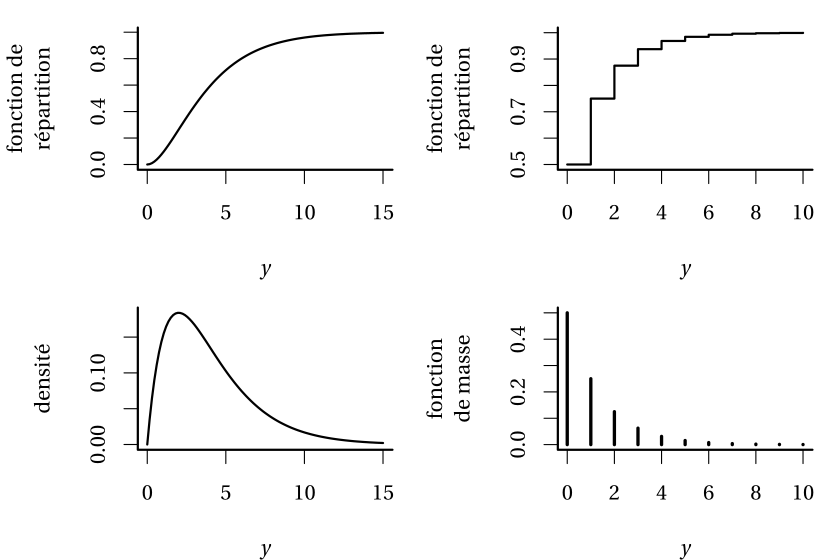
\includegraphics[width=0.85\textwidth,height=\textheight]{images/02-ttest-DF_illustration_fr.png}

}

\caption{\label{fig-distributions}Fonctions de répartition (panneau
supérieur) et fonctions de densité et de masse (panneau inférieur) pour
une loi continue (gauche) et discrète (droite).}

\end{figure}%

\end{definition}

Un premier cours de statistique débute souvent par la présentation de
statistiques descriptives comme la moyenne et l'écart-type. Ce sont des
estimateurs des moments (centrés), qui caractérisent la loi du phénomène
d'intérêt. Dans le cas de la loi normale unidimensionnelle, qui a deux
paramètres, l'espérance et la variance caractérisent complètement le
modèle.

\begin{definition}[Moments]\protect\hypertarget{def-moments}{}\label{def-moments}

Soit \(Y\) une variable aléatoire de fonction de densité (ou de masse)
\(f(x)\). On définit l'espérance d'une variable aléatoire \(Y\) comme
\begin{align*}
\mathsf{E}(Y)=\int_{\mathbb{R}} y f(y) \mathrm{d} y.
\end{align*} L'espérance est la « moyenne théorique», ou moment de
premier ordre : dans le cas discret,
\(\mu = \mathsf{E}(Y)=\sum_{y \in \mathcal{y}} y \mathsf{Pr}(y=y)\), où
\(\mathcal{Y}\) représente le support de la loi, à savoir les valeurs
qui peuvent prendre \(Y\). Plus généralement, l'espérance d'une fonction
\(g(y)\) pour une variable aléatoire \(Y\) est simplement l'intégrale de
\(g(y)\) pondérée par la densité \(f(y)\). De même, si l'intégrale est
convergente, la \textbf{variance} est \begin{align*}
\mathsf{Va}(Y)&=\int_{\mathbb{R}} (y-\mu)^2 f(y) \mathrm{d} y \\&=\mathsf{E}\{Y-\mathsf{E}(Y)\}^2 \\&= \mathsf{E}(Y^2) - \{\mathsf{E}(Y)\}^2.
\end{align*}

L'écart-type est défini comme la racine carrée de la variance,
\(\mathsf{sd}(Y)=\sqrt{\mathsf{Va}(Y)}\): elle est exprimé dans les
mêmes unités que celle de \(Y\) et donc plus facilement interprétable.

\begin{example}[]\protect\hypertarget{exm-moments-des}{}\label{exm-moments-des}

Considérons une variable aléatoire discrète \(Y\) pour la somme de deux
lancers de dés à six faces. L'espérance de \(g(Y)=Y^2\) est
\begin{align*}
\mathsf{E}(Y^2) &= (2^2 + 12^2) \times \frac{1}{36} + (3^2 + 11^2) \times  \frac{2}{36} + (4^2 + 10^2) \\&\;\times  \frac{3}{36} + (5^2 +9^2) \times  \frac{4}{36} + (6^2 + 8^2) \times  \frac{5}{36} \\& + 7^2 \times  \frac{6}{36}= \frac{329}{6}.
\end{align*}

\end{example}

La notion de moments peut être généralisé à des vecteurs. Si
\(\boldsymbol{Y}\) est un \(n\)-vecteur, comprenant par exemple dans le
cadre d'une régression des mesures d'un ensemble d'observations, alors
l'espérance est calculée composante par composante,

\begin{align*}
\mathsf{E}(\boldsymbol{Y}) &= \boldsymbol{\mu}=
\begin{pmatrix}
\mathsf{E}(Y_1) &
\cdots  &
\mathsf{E}(Y_n)
\end{pmatrix}^\top
\end{align*} tandis que la matrice \(n \times n\) de deuxième moments
centrés de \(\boldsymbol{Y}\), dite matrice de variance ou matrice de
\textbf{covariance}, est \begin{align*}
\mathsf{Va}(\boldsymbol{Y}) &= \boldsymbol{\Sigma} = \begin{pmatrix} \mathsf{Va}(Y_1) & \mathsf{Co}(Y_1, Y_2)  & \cdots & \mathsf{Co}(Y_1, Y_n) \\
\mathsf{Co}(Y_2, Y_1) & \mathsf{Va}(Y_2) & \ddots & \vdots \\
\vdots & \ddots & \ddots & \vdots \\
\mathsf{Co}(Y_n, Y_1) & \mathsf{Co}(Y_n, Y_2) &\cdots & \mathsf{Va}(Y_n)
\end{pmatrix}
\end{align*} Le \(i\)e élément diagonal de \(\boldsymbol{\Sigma}\),
\(\sigma_{ii}=\sigma_i^2\), est la variance de \(Y_i\), tandis que les
éléments hors de la diagonale, \(\sigma_{ij}=\sigma_{ji}\)
\((i \neq j)\), sont les covariances des paires \begin{align*}
\mathsf{Co}(Y_i, Y_j) = \int_{\mathbb{R}^2} (y_i-\mu_i)(y_j-\mu_j) f_{Y_i, Y_j}(y_i, y_j) \mathrm{d} y_i \mathrm{d} y_j.
\end{align*} Par construction, la matrice de covariance
\(\boldsymbol{\Sigma}\) est symmétrique. Il est d'usage de considérer la
relation deux-à-deux de variables standardisées, afin de séparer la
dépendance linéaire de la variabilité de chaque composante. La
\textbf{corrélation linéaire} entre \(Y_i\) et \(Y_j\) est
\begin{align*}
\rho_{ij}=\mathsf{Cor}(Y_i,Y_j)=\frac{\mathsf{Co}(Y_i, Y_j)}{\sqrt{\mathsf{Va}(Y_i)}\sqrt{\mathsf{Va}(Y_j)}}=\frac{\sigma_{ij}}{\sigma_i\sigma_j}.
\end{align*} La matrice de corrélation de \(\boldsymbol{Y}\) est une
matrice symmétrique \(n\times n\) avec des uns sur la diagonale et les
corrélations des pairs hors diagonale, \begin{align*}
\mathsf{Cor}(\boldsymbol{Y})=
\begin{pmatrix}
1 & \rho_{12} & \rho_{13} & \cdots & \rho_{1n}\\
\rho_{21} & 1 & \rho_{23} & \cdots & \rho_{2n} \\
\rho_{31} & \rho_{32} & 1 & \ddots & \rho_{3n} \\
\vdots & \vdots & \ddots & \ddots & \vdots \\
\rho_{n1} & \rho_{n2} & \rho_{n3} & \cdots & 1
\end{pmatrix}.
\end{align*} Nous modéliserons la matrice de covariance ou de
corrélation des données corrélées et longitudinales par individus du
même groupe (ou du même individu pour les mesures répétées) dans le
\href{donnees-longitudinales-correlees}{Chapitre 5}.

\end{definition}

\begin{definition}[Corrélation linéaire de
Pearson]\protect\hypertarget{def-correlation-Pearson}{}\label{def-correlation-Pearson}

Le coefficient de corrélation linéaire entre \(X_j\) et \(X_k\), que
l'on note \(r_{j, k}\), cherche à mesurer la force de la relation
linéaire entre deux variables, c'est-à-dire à quantifier à quel point
les observations sont alignées autour d'une droite. Le coefficient de
corrélation est \begin{align*}
r_{j, k} &= \frac{\widehat{\mathsf{Co}}(X_j, X_k)}{\{\widehat{\mathsf{Va}}(X_j) \widehat{\mathsf{Va}}(X_k)\}^{1/2}}
%\\&=\frac{\sum_{i=1}^n (x_{i, j}-\overline{x}_j)(x_{i, k} -\overline{x}_{k})}{\left\{\sum_{i=1}^n (x_{i, j}-\overline{x}_j)^2 \sum_{i=1}^n(x_{i, k} -\overline{x}_{k})^2\right\}^{1/2}}
\end{align*}

Les propriétés les plus importantes du coefficient de corrélation
linéaire \(r\) sont les suivantes:

\begin{enumerate}
\def\labelenumi{\arabic{enumi})}
\tightlist
\item
  \(-1 \leq r \leq 1\);
\item
  \(r=1\) (respectivement \(r=-1\)) si et seulement si les \(n\)
  observations sont exactement alignées sur une droite de pente positive
  (négative). C'est-à-dire, s'il existe deux constantes \(a\) et \(b>0\)
  (\(b<0\)) telles que \(y_i=a+b x_i\) pour tout \(i=1, \ldots, n\).
\end{enumerate}

Règle générale,

\begin{itemize}
\tightlist
\item
  Le signe de la corrélation détermine l'orientation de la pente
  (négative ou positive)
\item
  Plus la corrélation est près de 1 en valeur absolue, plus les points
  auront tendance à être alignés autour d'une droite.
\item
  Lorsque la corrélation est presque nulle, les points n'auront pas
  tendance à être alignés autour d'une droite. Il est très important de
  noter que cela n'implique pas qu'il n'y a pas de relation entre les
  deux variables. Cela implique seulement qu'il n'y a pas de
  \textbf{relation linéaire} entre les deux variables.
\end{itemize}

\end{definition}

La Figure~\ref{fig-datasaurus} montre bien ce dernier point: ces jeux de
données ont la même corrélation linéaire (quasi-nulle) et donc la même
droite de régression, mais ne sont clairement pas indépendantes
puisqu'elles permettent de dessiner un dinosaure ou une étoile.

\begin{figure}[ht!]

\centering{

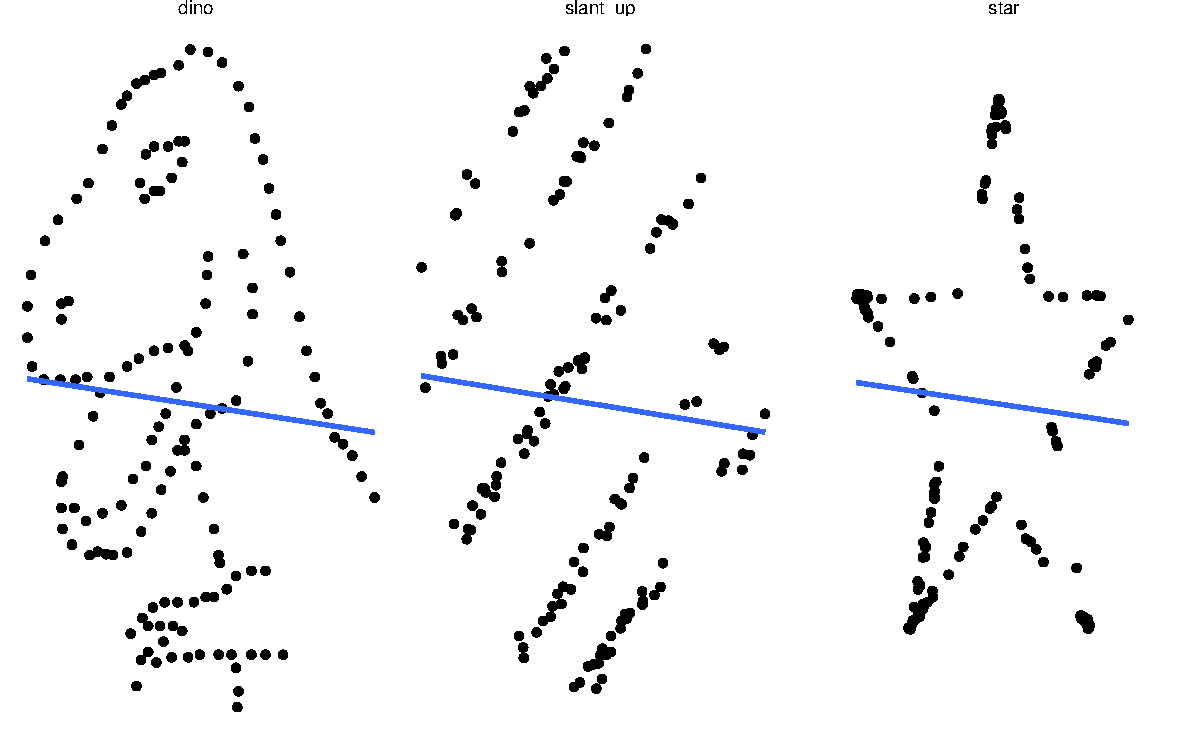
\includegraphics[width=0.85\textwidth,height=\textheight]{introduction_files/figure-pdf/fig-datasaurus-1.pdf}

}

\caption{\label{fig-datasaurus}Trois jeux de données de
\texttt{datasauRus}, avec une corrélation linéaire de -0.06 et des
statistiques descriptives moyenne, écart-type, etc. identiques pour
chaque jeu de données.}

\end{figure}%

\begin{definition}[Biais]\protect\hypertarget{def-biais}{}\label{def-biais}

Le biais d'un estimateur \(\hat{\theta}\) pour un paramètre \(\theta\)
est \begin{align*}
\mathsf{biais}(\hat{\theta})=\mathsf{E}(\hat{\theta})- \theta
\end{align*} L'estimateur est non biaisé si
\(\mathsf{biais}(\hat{\theta})=0\).

\end{definition}

\begin{example}[Estimateurs sans
biais]\protect\hypertarget{exm-estimateurs-non-biaises}{}\label{exm-estimateurs-non-biaises}

L'estimateur sans biais de l'espérance de \(Y\) pour un échantillon
aléatoire simple \(Y_1, \ldots, Y_n\) est la moyenne empirique
\(\overline{Y}_n = n^{-1} \sum_{i=1}^n Y_i\) et celui de la variance
\(S_n = (n-1)^{-1} \sum_{i=1}^n (Y_i-\overline{Y})^2\).

\end{example}

Un estimateur sans biais est souhaitable, mais pas toujours optimal.
Quelquefois, il n'existe pas d'estimateur non-biaisé pour un paramètre!
Dans plusieurs cas, on cherche un estimateur qui minimise l'erreur
quadratique moyenne.

Souvent, on cherche à balancer le biais et la variance: rappelez-vous
qu'un estimateur est une variable aléatoire (étant une fonction de
variables aléatoires) et qu'il est lui-même variable: même s'il est sans
biais, la valeur numérique obtenue fluctuera d'un échantillon à l'autre.

\begin{definition}[Erreur quadratique
moyenne]\protect\hypertarget{def-eqm}{}\label{def-eqm}

On peut chercher un estimateur qui minimise l'erreur quadratique
moyenne, \begin{align*}
\mathsf{EQM}(\hat{\theta}) = \mathsf{E}\{(\hat{\theta}-\theta)^2\}=\mathsf{Va}(\hat{\theta}) + \{\mathsf{E}(\hat{\theta})\}^2.
\end{align*} Cette fonction objective est donc un compromis entre le
carré du biais et la variance de l'estimateur.

\end{definition}

La plupart des estimateurs que nous considérerons dans le cadre du cours
sont des estimateurs du maximum de vraisemblance. Ces derniers sont
asymptotiquement efficaces, c'est-à-dire qu'ils minimisent l'erreur
quadratique moyenne parmi tous les estimateurs possibles quand la taille
de l'échantillon est suffisamment grande. Ils ont également d'autre
propriétés qui les rendent attractifs comme choix par défaut pour
l'estimation. Il ne sont pas nécessairement sans biais

\section{Loi discrètes}\label{loi-discruxe8tes}

Plusieurs lois aléatoires décrivent des phénomènes physiques simples et
ont donc une justification empirique; on revisite les distributions ou
loi discrètes les plus fréquemment couvertes.

\begin{definition}[Loi de
Bernoulli]\protect\hypertarget{def-loibern}{}\label{def-loibern}

On considère un phénomène binaire, comme le lancer d'une pièce de
monnaie (pile/face). De manière générale, on associe les deux
possibilités à succès/échec et on suppose que la probabilité de
``succès'' est \(p\). Par convention, on représente les échecs (non) par
des zéros et les réussites (oui) par des uns. Donc, si la variable \(Y\)
vaut \(0\) ou \(1\), alors \(\mathsf{Pr}(Y=1)=p\) et la probabilité
complémentaire est \(\mathsf{Pr}(Y=0)=1-p\). La fonction de masse de la
\href{https://fr.wikipedia.org/wiki/Loi_de_Bernoulli}{loi Bernoulli}
s'écrit de façon plus compacte \begin{align*}
\mathsf{Pr}(Y=y) = p^y (1-p)^{1-y}, \quad y=0, 1.
\end{align*}

\end{definition}

Un calcul rapide montre que \(\mathsf{E}(Y)=p\) et
\(\mathsf{Va}(Y)=p(1-p)\). Effectivement, \begin{align*}
\mathsf{E}(Y) = \mathsf{E}(Y^2) = p \cdot 1 + (1-p) \cdot 0 = p.
\end{align*}

Voici quelques exemples de questions de recherches comprenant une
variable réponse binaire:

\begin{itemize}
\tightlist
\item
  est-ce qu'un client potentiel a répondu favorablement à une offre
  promotionnelle?
\item
  est-ce qu'un client est satisfait du service après-vente?
\item
  est-ce qu'une firme va faire faillite au cours des trois prochaines
  années?
\item
  est-ce qu'un participant à une étude réussit une tâche assignée?
\end{itemize}

Plus généralement, on aura accès à des données aggrégées.

\begin{example}[Loi
binomiale]\protect\hypertarget{exm-loibinom}{}\label{exm-loibinom}

Si les données représentent la somme d'événements Bernoulli
indépendants, la loi du nombre de réussites \(Y\) pour un nombre
d'essais donné \(m\) est dite
\href{https://fr.wikipedia.org/wiki/Loi_binomiale}{binomiale}, dénotée
\(\mathsf{Bin}(m, p)\); sa fonction de masse est \begin{align*}
\mathsf{Pr}(Y=y) = \binom{m}{y}p^y (1-p)^{m-y}, \quad y=0, 1, \ldots, m.
\end{align*} La vraisemblance pour un échantillon de la loi binomiale
est (à constante de normalisation près qui ne dépend pas de \(p\)) la
même que pour un échantillon aléatoire de \(m\) variables Bernoulli
indépendantes. L'espérance d'une variable binomiale est
\(\mathsf{E}(Y)=mp\) et la variance \(\mathsf{Va}(Y)=mp(1-p)\).

\end{example}

On peut ainsi considérer le nombre de personnes qui ont obtenu leur
permis de conduire parmi \(m\) candidat(e)s ou le nombre de clients sur
\(m\) qui ont passé une commande de plus de 10\$ dans un magasin.

Plus généralement, on peut considérer des variables de dénombrement qui
prennent des valeurs entières. Parmi les exemples de questions de
recherches comprenant une variable réponse de dénombrement:

\begin{itemize}
\tightlist
\item
  le nombre de réclamations faites par un client d'une compagnie
  d'assurance au cours d'une année.
\item
  le nombre d'achats effectués par un client depuis un mois.
\item
  le nombre de tâches réussies par un participant lors d'une étude.
\end{itemize}

\begin{example}[Loi de
Poisson]\protect\hypertarget{exm-loipoisson}{}\label{exm-loipoisson}

Si la probabilité d'un événement Bernoulli est petite et qu'il est rare
d'obtenir un succès dans le sens où \(mp \to \lambda\) quand le nombre
d'essais \(m\) augmente, alors le nombre de succès suit
approximateivement une loi de Poisson de fonction de masse
\begin{align*}
\mathsf{Pr}(Y=y) = \frac{\exp(-\lambda)\lambda^y}{\Gamma(y+1)}, \quad y=0, 1, 2, \ldots
\end{align*} où \(\Gamma(\cdot)\) dénote la fonction gamma, et
\(\Gamma(y+1) = y!\) si \(y\) est un entier. Le paramètre \(\lambda\) de
la loi de Poisson représente à la fois l'espérance et la variance de la
variable, c'est-à-dire que \(\mathsf{E}(Y)=\mathsf{Va}(Y)=\lambda\).

\end{example}

\begin{example}[Loi binomiale
négative]\protect\hypertarget{exm-loibinneg}{}\label{exm-loibinneg}

On considère une série d'essais Bernoulli de probabilité de succès \(p\)
jusqu'à l'obtention de \(m\) succès. Soit \(Y\), le nombre d'échecs:
puisque la dernière réalisation doit forcément être un succès, mais que
l'ordre des succès/échecs précédents n'importe pas, la fonction de masse
de la loi binomiale négative est \begin{align*}
\mathsf{Pr}(Y=y)= \binom{m-1+y}{y} p^m (1-p)^{y}.
\end{align*}

La loi binomiale négative apparaît également si on considère la loi
non-conditionnelle du modèle hiérarchique gamma-Poisson, dans lequel on
suppose que le paramètre de la moyenne de la loi Poisson est aussi
aléatoire, c'est-à-dire
\(Y \mid \Lambda=\lambda \sim \mathsf{Po}(\lambda)\) et \(\Lambda\) suit
une loi gamma de paramètre de forme \(r\) et de paramètre d'échelle
\(\theta\), dont la densité est \begin{align*}
f(x) = \theta^{-r}x^{r-1}\exp(-x/\theta)/\Gamma(r).\end{align*} Le
nombre d'événements suit alors une loi binomiale négative.

La paramétrisation la plus courante pour la modélisation est légèrement
différente: pour un paramètre \(r>0\) (pas forcément entier), on écrit
la fonction de masse \begin{align*}
\mathsf{Pr}(Y=y)=\frac{\Gamma(y+r)}{\Gamma(y+1)\Gamma(r)} \left(\frac{r}{r + \mu} \right)^{r} \left(\frac{\mu}{r+\mu}\right)^y,
\end{align*} où \(\Gamma\) dénote la fonction gamma. Dans cette
paramétrisation, la moyenne théorique et la variance sont
\(\mathsf{E}(Y)=\mu\) et \(\mathsf{Va}(Y)=\mu+k\mu^2\), où \(k=1/r\). La
variance d'une variable binomiale négative est \emph{supérieure} à sa
moyenne et le modèle est utilisé comme alternative à la loi de Poisson
pour modéliser la surdispersion.

\end{example}

\section{Lois continues}\label{lois-continues}

On considère plusieurs lois de variables aléatoires continues; certaines
servent de lois pour des tests d'hypothèse et découlent du théorème
central limite (notamment les lois normales, Student, Fisher ou \(F\),
et khi-deux).

\begin{definition}[Loi
beta]\protect\hypertarget{def-loibeta}{}\label{def-loibeta}

La loi beta \(\mathsf{Beta}(\alpha, \beta)\) est une loi sur
l'intervalle \([0,1]\) avec paramètres de forme \(\alpha>0\) et
\(\beta>0\). Sa densité est \begin{align*}
f(x) = \frac{\Gamma(\alpha)\Gamma(\beta)}{\Gamma(\alpha+\beta)}x^{\alpha-1}(1-x)^{1-\beta}, \qquad x \in [0,1].
\end{align*} Le cas \(\alpha=\beta=1\), dénotée également
\(\mathsf{unif}(0,1)\), correspond à la loi standard uniforme.

\begin{figure}[ht!]

\centering{

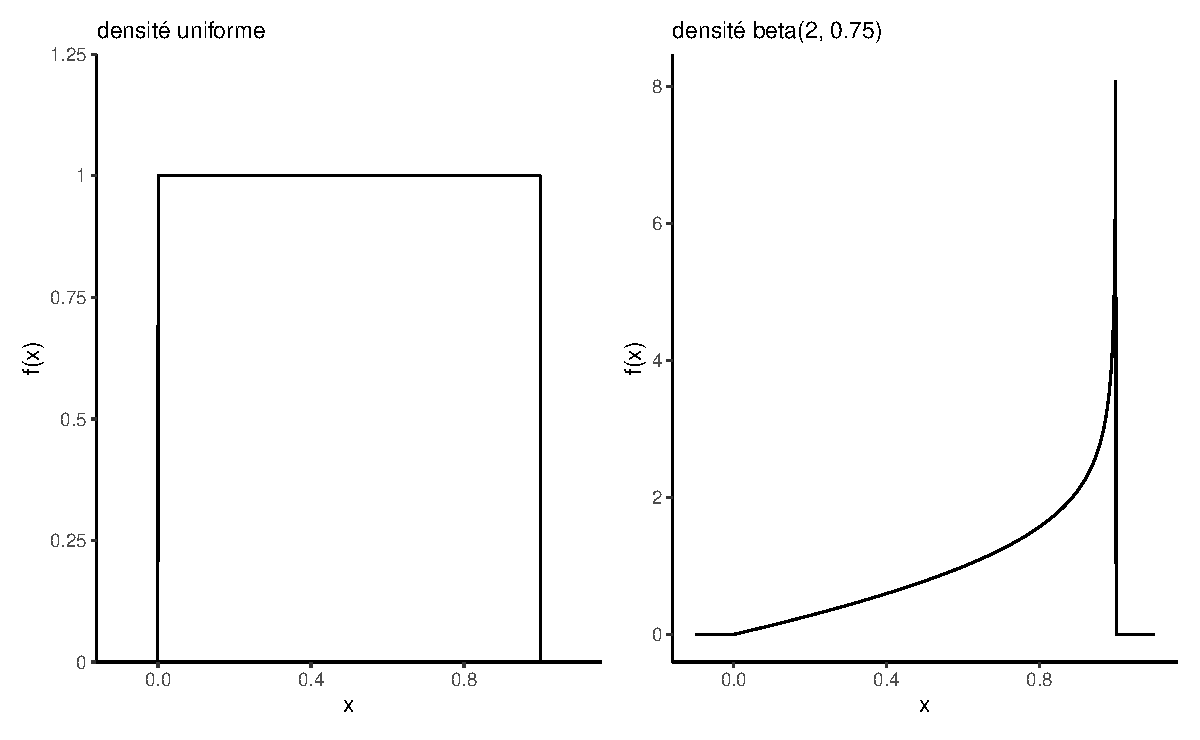
\includegraphics[width=0.85\textwidth,height=\textheight]{introduction_files/figure-pdf/fig-densite-beta-1.pdf}

}

\caption{\label{fig-densite-beta}Fonctions de densité de lois uniformes
et beta(2, 3/4) sur l'intervalle {[}0,1{]}.}

\end{figure}%

\end{definition}

\begin{definition}[Loi
exponentielle]\protect\hypertarget{def-loiexpo}{}\label{def-loiexpo}

La loi exponentielle figure de manière proéminente dans l'étude des
temps d'attente pour les phénomènes Poisson et en analyse de survie. Une
caractéristique clé de la loi est son absence de mémoire:
\(\Pr(Y \geq y + u \mid Y > u) = \Pr(Y > u)\) pour \(Y > 0\) et
\(y, u>0\).

La fonction de répartition de la loi exponentielle
\(Y \sim \mathsf{Exp}(\beta)\) où \(\beta>0\), est
\(F(x) = 1-\exp(-\beta x)\) et sa fonction de densité est
\(f(x) =\beta\exp(-\beta x)\) pour \(x >0\). La moyenne théorique de la
loi est \(\beta\).

\end{definition}

\begin{definition}[Loi
normale]\protect\hypertarget{def-loinormale}{}\label{def-loinormale}

De loin la plus continue des distributions, la loi normale intervient
dans le théorème central limite, qui dicte le comportement aléatoire de
la moyenne de grand échantillons. La loi normale est pleinement
caractérisée par son espérance \(\mu \in \mathbb{R}\) et son écart-type
\(\sigma>0\). Loi symmétrique autour de \(\mu\), c'est une famille de
localisation et d'échelle. Sa fonction de densité, \begin{align*}
f(x) = (2\pi\sigma^2)^{-1/2} \exp \left\{ - \frac{(x-\mu)^2}{2\sigma^2}\right\}, \qquad x \in \mathbb{R}.
\end{align*} en forme de cloche, est symmétrique autour de \(\mu\), qui
est aussi le mode de la distribution.

\begin{figure}[ht!]

\centering{

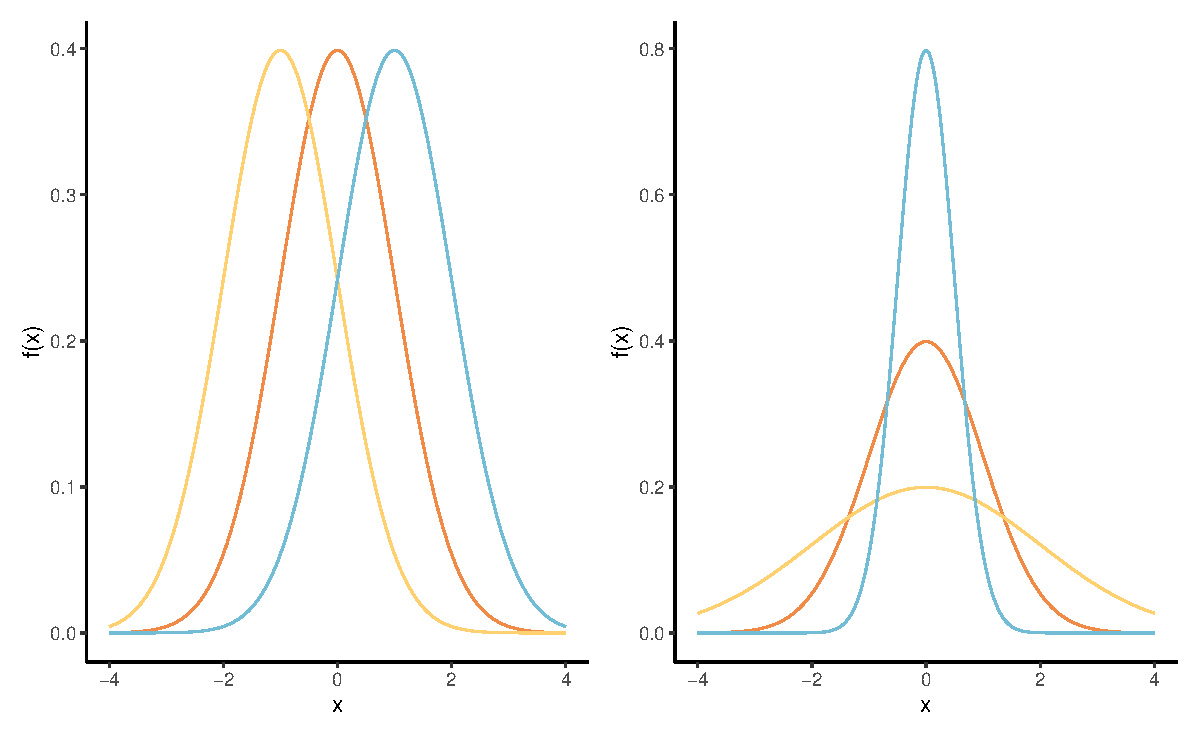
\includegraphics[width=0.85\textwidth,height=\textheight]{introduction_files/figure-pdf/fig-normal-loc-echelle-1.pdf}

}

\caption{\label{fig-normal-loc-echelle}Densités de loi normales avec des
paramètres de moyenne différents (gauche) et des paramètres d'échelle
différents (droite).}

\end{figure}%

The distribution function of the normal distribution is not available in
closed-form. La loi normale est une famille de localisation échelle: si
\(Y \sim \mathsf{normale}(\mu, \sigma^2)\), alors
\(Z = (Y-\mu)/\sigma \sim \mathsf{normale}(0,1)\). Inversement, si
\(Z \sim \mathsf{normale}(0,1)\), alors
\(Y = \mu + \sigma Z \sim \mathsf{normale}(\mu, \sigma^2)\).

Nous verrons aussi l'extension multidimensionnelle de la loi normale: un
\(d\) vecteur
\(\boldsymbol{Y} \sim \mathsf{normal}_d(\boldsymbol{\mu}, \boldsymbol{\Sigma})\)
admet une fonction de densité égale à \begin{align*}
f(\boldsymbol{x}) = (2\pi)^{-d/2} |\boldsymbol{\Sigma}|^{-1/2} \exp \left\{ - \frac{1}{2} (\boldsymbol{x}-\boldsymbol{\mu})^\top \boldsymbol{\Sigma}^{-1}(\boldsymbol{x}-\boldsymbol{\mu})\right\}
\end{align*}

Le vecteur de moyenne \(\boldsymbol{\mu}\) contient l'espérance de
chaque composante, tandis que \(\boldsymbol{\Sigma}\) est la matrice de
covariance de \(\boldsymbol{Y}\). Une propriété unique à la loi normale
(muldimensionnelle) est le lien entre indépendance et matrice de
covariance: si \(Y_i\) et \(Y_j\) sont indépendants, alors l'entrée
\((i,j)\) hors diagonale de \(\boldsymbol{\Sigma}\) est nulle.

\end{definition}

Les trois lois suivantes ne sont pas couvertes dans les cours
d'introduction, mais elles interviennent régulièrement dans les cours de
mathématique statistique et serviront d'étalon de mesure pour déterminer
si les statistiques de test sont extrêmes sous l'hypothèse nulle.

\begin{definition}[Loi
khi-deux]\protect\hypertarget{def-loikhideux}{}\label{def-loikhideux}

La loi de khi-deux avec \(\nu>0\) degrés de liberté, dénotée
\(\chi^2_{\nu}\) ou \(\mathsf{khi-deux}(\nu)\) joue un rôle important en
statistique. Sa densité est \begin{align*}
f(x; \nu) = \frac{1}{2^{\nu/2}\Gamma(\nu/2)}x^{\nu/2-1}\exp(-x/2),\qquad x >0.
\end{align*} Elle est obtenue pour \(\nu\) entier en prenant la somme de
variables normales centrées et réduites au carré: si
\(Y_i \stackrel{\mathrm{iid}}{\sim}\mathsf{normale}(0,1)\) pour
\(i=1, \ldots, k\), alors \(\sum_{i=1}^k Y_i^2 \sim \chi^2_k\).
L'espérance de la loi \(\chi^2_k\) est \(k\).

\end{definition}

Si on considère un échantillon aléatoire et identiquement distribution
de \(n\) observations de lois normales, alors la variance empirique
repondérée satisfait \((n-1)S^2/\sigma^2 \sim \chi^2_{n-1}\).

\begin{definition}[Loi
Student-\(t\)]\protect\hypertarget{def-loistudent}{}\label{def-loistudent}

La loi Student-\(t\) avec \(\nu>0\) degrés de liberté est une famille de
localisation et d'échelle de densité symmétrique. On la dénote
\(\mathsf{Student}(\nu)\) dans le cas centré réduit.

Son nom provient d'un article de William Gosset sous le pseudonyme
Student (\citeproc{ref-Student:1908}{Gosset 1908}), qui a introduit la
loi comme approximation au comportement de la statistique \(t\). La
densité d'une loi Student standard avec \(\nu\) degrés de liberté est
\begin{align*}
f(y; \nu) = \frac{\Gamma \left( \frac{\nu+1}{2}\right)}{\Gamma\left(\frac{\nu}{2}\right)
\sqrt{\nu\pi}}\left(1+\frac{y^{2}}{\nu}\right)^{-\frac{\nu+1}{2}}.
\end{align*} La loi a des ailes à décroissance polynomiale, est
symmétrique autour de zéro et unimodale. Quand \(\nu \to \infty\), on
recouvre une loi normale, mais les ailes sont plus lourdes que la loi
normale. Effectivement, seuls les \(\nu-1\) premiers moments de la
distribution existent: la loi \(\mathsf{Student}(2)\) n'a pas de
variance.

Si les \(n\) observations indépendantes et identiquement distribuées
\(Y_i \sim \mathsf{normale}(\mu, \sigma^2)\), alors la moyenne empirique
centrée, divisée par la variance empirique, \((\overline{Y}-\mu)/S^2\),
suit une loi Student-\(t\) avec \(n-1\) degrés de liberté.

\begin{figure}[ht!]

\centering{

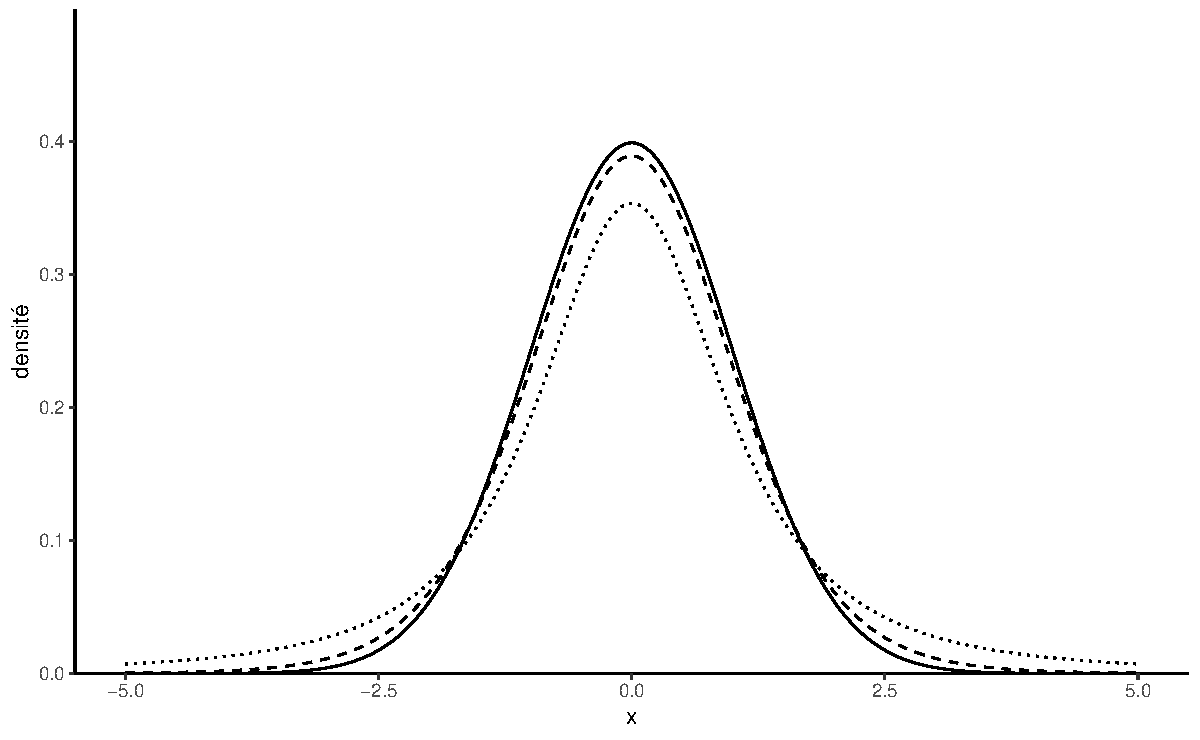
\includegraphics[width=0.5\textwidth,height=\textheight]{introduction_files/figure-pdf/fig-densite-Student-1.pdf}

}

\caption{\label{fig-densite-Student}Comparaison de la densité
Student-\(t\) versus normale pour différents degrés de liberté avec
\(\nu=2\) (pointillé), \(\nu=10\) (traitillé) et la loi normale
(\(\nu = \infty)\).}

\end{figure}%

\end{definition}

\begin{definition}[Loi de
Fisher]\protect\hypertarget{def-loiF}{}\label{def-loiF}

La loi de Fisher, ou loi \(F\), sert à déterminer le comportement en
grand échantillon de statistiques de test pour la comparaison de
plusieurs moyennes (analyse de variance) sous un postulat de normalité
des observations.

La loi \(F\), dite de Fisher et dénotée
\(\mathsf{Fisher}(\nu_1, \nu_2)\), est obtenue en divisant deux
variables khi-deux indépendantes de degrés de liberté \(\nu_1\) et
\(\nu_2\). Spécifiquement, si \(Y_1 \sim \chi^2_{\nu_1}\) et
\(Y_2 \sim \chi^2_{\nu_2}\), alors \begin{align*}
F = \frac{Y_1/\nu_1}{Y_2/\nu_2} \sim \mathsf{Fisher}(\nu_1, \nu_2)
\end{align*}

La loi de Fisher tend vers une loi \(\chi^2_{\nu_1}\) quand
\(\nu_2 \to \infty\).

\end{definition}

\section{Graphiques}\label{graphiques}

Cette section sert à réviser les principales représentations graphiques
de jeux de données selon la catégorie des variables.

Le principal type de graphique pour représenter la distribution d'une
variable catégorielle est le diagramme en bâtons, dans lequel la
fréquence de chaque catégorie est présentée sur l'axe des ordonnées
(\(y\)) en fonction de la modalité, sur l'axe des abscisses (\(x\)), et
ordonnées pour des variables ordinales. Cette représentation est en tout
point supérieur au
\href{http://www.perceptualedge.com/articles/08-21-07.pdf}{diagramme en
camembert}, une engeance répandu qui devrait être honnie (notamment
parce que l'humain juge mal les différences d'aires, qu'une simple
rotation change la perception du graphique et qu'il est difficile de
mesurer les proportions) --- ce n'est pas de la tarte!

\begin{figure}[ht!]

\centering{

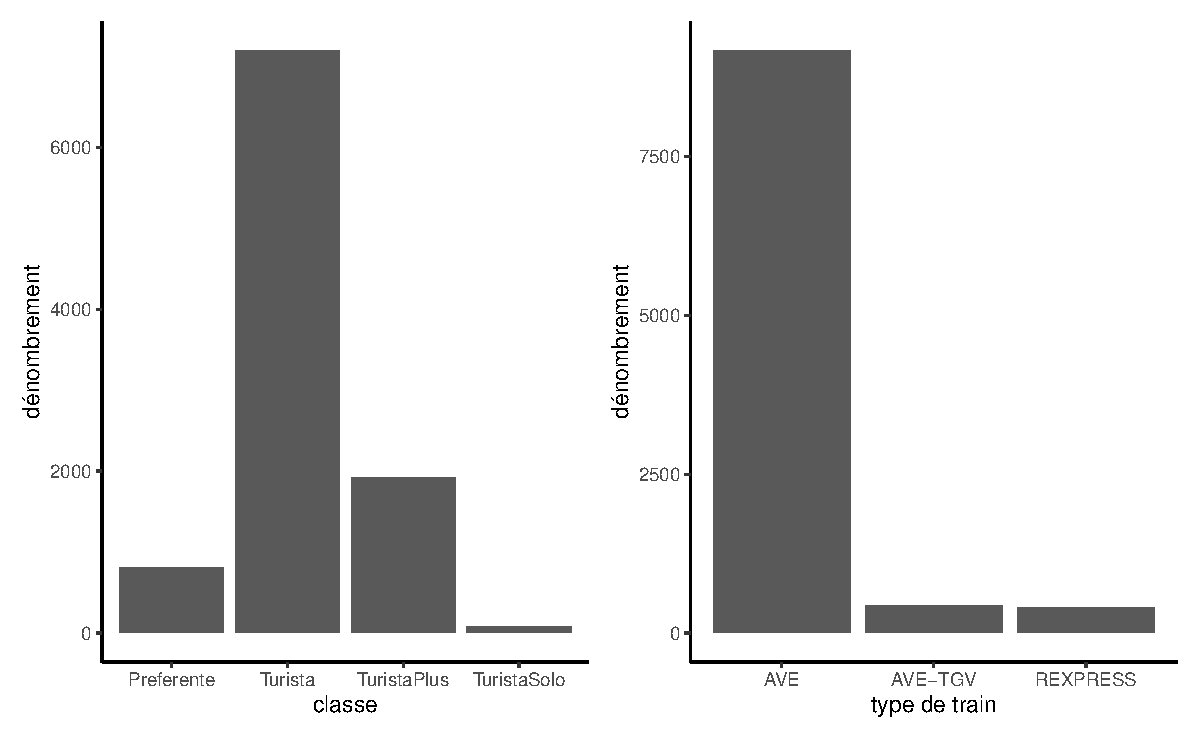
\includegraphics[width=0.85\textwidth,height=\textheight]{introduction_files/figure-pdf/fig-barplotrenfe-1.pdf}

}

\caption{\label{fig-barplotrenfe}Diagramme en bâtons pour la classe des
billets de trains du jeu de données Renfe.}

\end{figure}%

Puisque les variables continues peuvent prendre autant de valeurs
distinctes qu'il y a d'observations, on ne peut simplement compter le
nombre d'occurrence par valeur unique. On regroupera plutôt dans un
certain nombre d'intervalle, en discrétisant l'ensemble des valeurs en
classes pour obtenir un histogramme. Le nombre de classes dépendra du
nombre d'observations si on veut que l'estimation ne soit pas impactée
par le faible nombre d'observations par classe: règle générale, le
nombre de classes ne devrait pas dépasser \(\sqrt{n}\), où \(n\) est le
nombre d'observations de l'échantillon. On obtiendra la fréquence de
chaque classe, mais si on normalise l'histogramme (de façon à ce que
l'aire sous les bandes verticales égale un), on obtient une
approximation discrète de la fonction de densité. Faire varier le nombre
de classes permet parfois de faire apparaître des caractéristiques de la
variable (notamment la multimodalité, l'asymmétrie et les arrondis).

Puisque qu'on groupe les observations en classe pour tracer
l'histogramme, il est difficile de voir l'étendue des valeurs que prenne
la variable: on peut rajouter des traits sous l'histogramme pour
représenter les valeurs uniques prises par la variable, tandis que la
hauteur de l'histogramme nous renseigne sur leur fréquence relative.

\begin{figure}[ht!]

\centering{

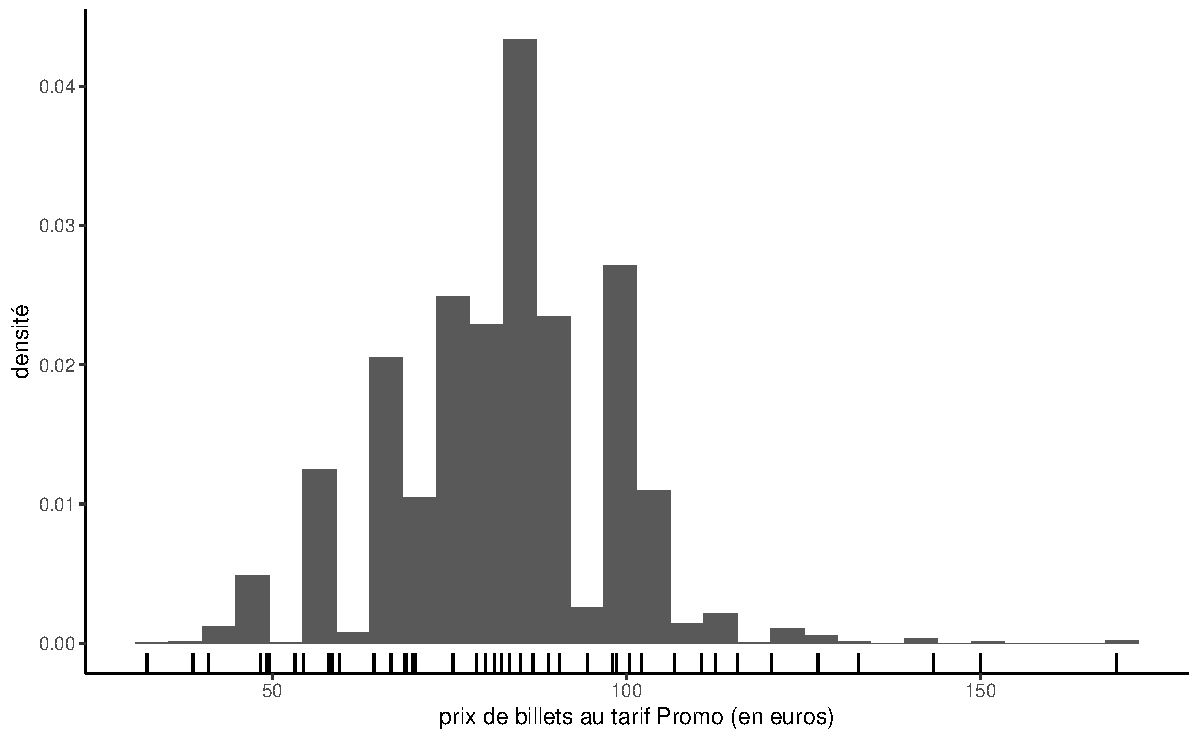
\includegraphics[width=0.85\textwidth,height=\textheight]{introduction_files/figure-pdf/fig-histrenfe-1.pdf}

}

\caption{\label{fig-histrenfe}Histogramme du prix des billets au tarif
Promo de trains du jeu de données Renfe}

\end{figure}%

\begin{definition}[Boîte à
moustaches]\protect\hypertarget{def-boxplot}{}\label{def-boxplot}

Elle représente graphiquement cinq statistiques descriptives.

\begin{itemize}
\tightlist
\item
  La boîte donne les 1e, 2e et 3e quartiles \(q_1, q_2, q_3\). Il y a
  donc 50\% des observations sont au-dessus/en-dessous de la médiane
  \(q_2\) qui sépare en deux la boîte.
\item
  La longueur des moustaches est moins de \(1.5\) fois l'écart
  interquartile \(q_3-q_1\) (tracée entre 3e quartile et le dernier
  point plus petit que \(q_3+1.5(q_3-q_1)\), etc.)
\item
  Les observations au-delà des moustaches sont encerclées. Notez que
  plus le nombre d'observations est élevé, plus le nombres de valeurs
  aberrantes augmente. C'est un défaut de la boîte à moustache, qui a
  été conçue pour des jeux de données qui passeraient pour petits selon
  les standards actuels.
\end{itemize}

\begin{figure}[ht!]

{\centering 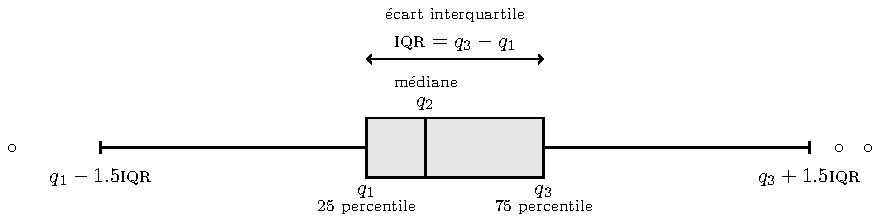
\includegraphics[width=0.85\textwidth,height=\textheight]{images/01-intro-boiteamoustache.pdf}

}

\caption{Boîte à moustache.}

\end{figure}%

\end{definition}

On peut représenter la distribution d'une variable réponse continue en
fonction d'une variable catégorielle en traçant une boîte à moustaches
pour chaque catégorie et en les disposant côte-à-côte. Une troisième
variable catégorielle peut être ajoutée par le biais de couleurs, comme
dans la Figure~\ref{fig-histboxplot}.

\begin{figure}[ht!]

\centering{

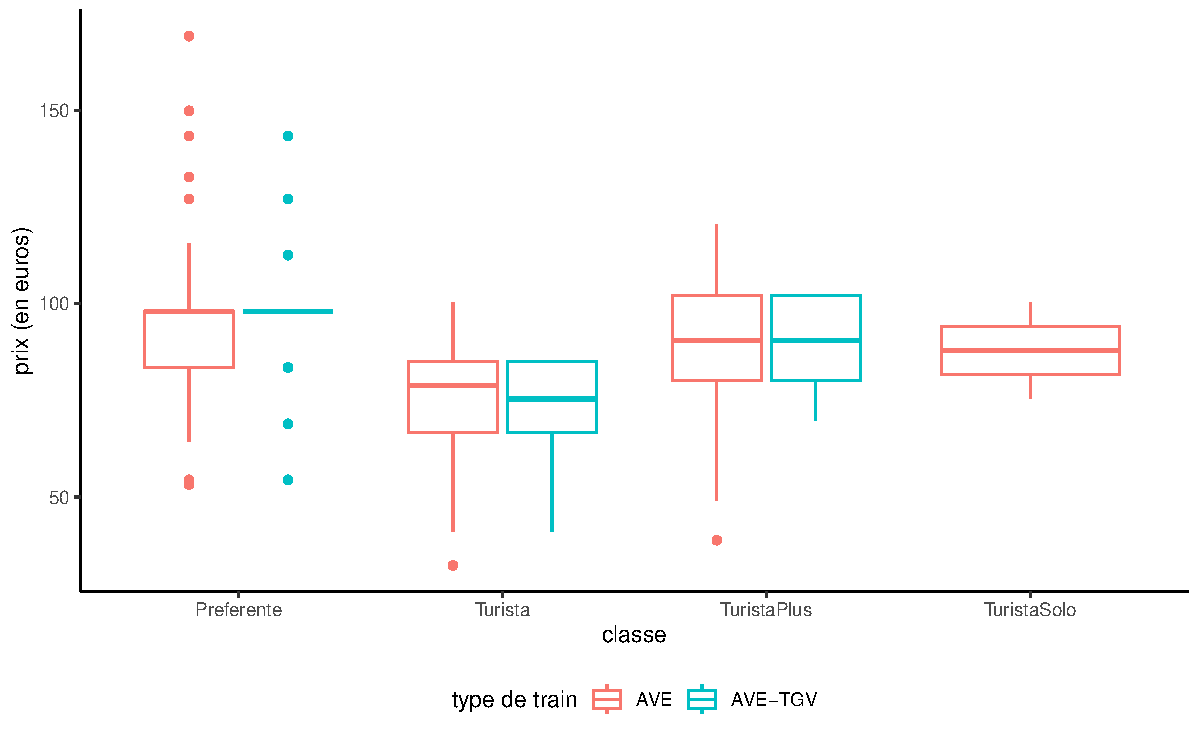
\includegraphics[width=0.85\textwidth,height=\textheight]{introduction_files/figure-pdf/fig-histboxplot-1.pdf}

}

\caption{\label{fig-histboxplot}Boîte à moustaches du prix des billets
au tarif Promo en fonction de la classe pour le jeu de données Renfe.}

\end{figure}%

Si on veut représenter la covariabilité de deux variables continues, on
utilise un nuage de points où chaque variable est représentée sur un axe
et chaque observation donne la coordonnée des points. Si la
représentation graphique est dominée par quelques valeurs très grandes,
une transformation des données peut être utile: vous verrez souvent des
données positives à l'échelle logarithmique. Si le nombre d'observations
est très grand, il devient difficile de distinguer quoi que ce soit. On
peut alors ajouter de la transparence ou regrouper des données en
compartiments bidimensionnels (un histogramme bidimensionnel), dont la
couleur représente la fréquence de chaque compartiment. Le paneau gauche
de Figure~\ref{fig-nuagedepoints} montre un nuage de points de 100
observations simulées, tandis que celui de droite représente des
compartiments hexagonaux contenant 10 000 points.

\begin{figure}[ht!]

\centering{

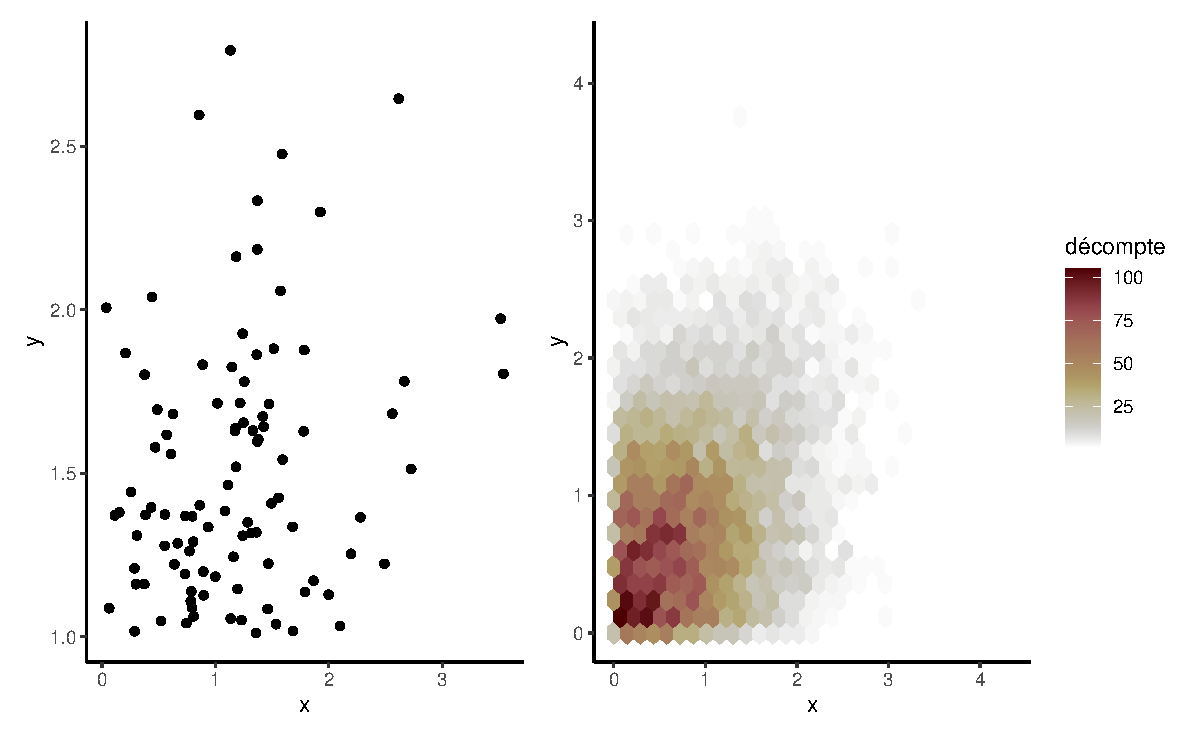
\includegraphics[width=0.85\textwidth,height=\textheight]{introduction_files/figure-pdf/fig-nuagedepoints-1.pdf}

}

\caption{\label{fig-nuagedepoints}Nuage de points (gauche) et diagramme
hexagonal (droite) pour des données simulées.}

\end{figure}%

Si on ajuste un modèle à des données, il convient de vérifier la qualité
de l'ajustement et l'adéquation du modèle, par exemple graphiquement.

\begin{definition}[Diagrammes
quantiles-quantiles]\protect\hypertarget{def-diagramme-qq}{}\label{def-diagramme-qq}

Le diagramme quantile-quantile sert à vérifier l'adéquation du modèle et
découle du constat suivant: si \(Y\) est une variable aléatoire continue
et \(F\) sa fonction de répartition, alors l'application
\(F(Y) \sim \mathsf{unif}(0,1)\), une loi uniforme standard. De la même
façon, appliquer la fonction quantile à une variable uniforme permet de
simuler de la loi \(F\), et donc \(F^{-1}(U)\). Supposons un échantillon
uniforme de taille \(n\). On peut démontrer que, pour des variables
continues, les statistiques d'ordre \(U_{(1)} \leq \cdots \leq U_{(n)}\)
ont une loi marginale beta, avec
\(U_{(k)} \sim \mathsf{Beta}(k, n+1-k)\) d'espérance \(k/(n+1)\).

Les paramètres de la loi \(F\) sont inconnus, mais on peut obtenir un
estimateur \(\widehat{F}\) et appliquer la transformation inverse pour
obtenir une variable approximativement uniforme. Un diagramme
quantile-quantile représente les données en fonction des moments des
statistiques d'ordre transformées

\begin{itemize}
\tightlist
\item
  sur l'axe des abscisses, les quantiles théoriques
  \(\widehat{F}^{-1}\{\mathrm{rang}(Y_i)/(n+1)\}\)
\item
  sur l'axe des ordonnées, les quantiles empiriques \(Y_i\)
\end{itemize}

Si le modèle est adéquat, les valeurs ordonnées devraient suivre une
droite de pente unitaire qui passe par l'origine. Le diagramme
probabilité-probabilité représente plutôt les données à l'échelle
uniforme \(\{\mathrm{rang}(Y_i)/(n+1), \widehat{F}(Y_i)\}\).

\end{definition}

\begin{figure}[ht!]

\centering{

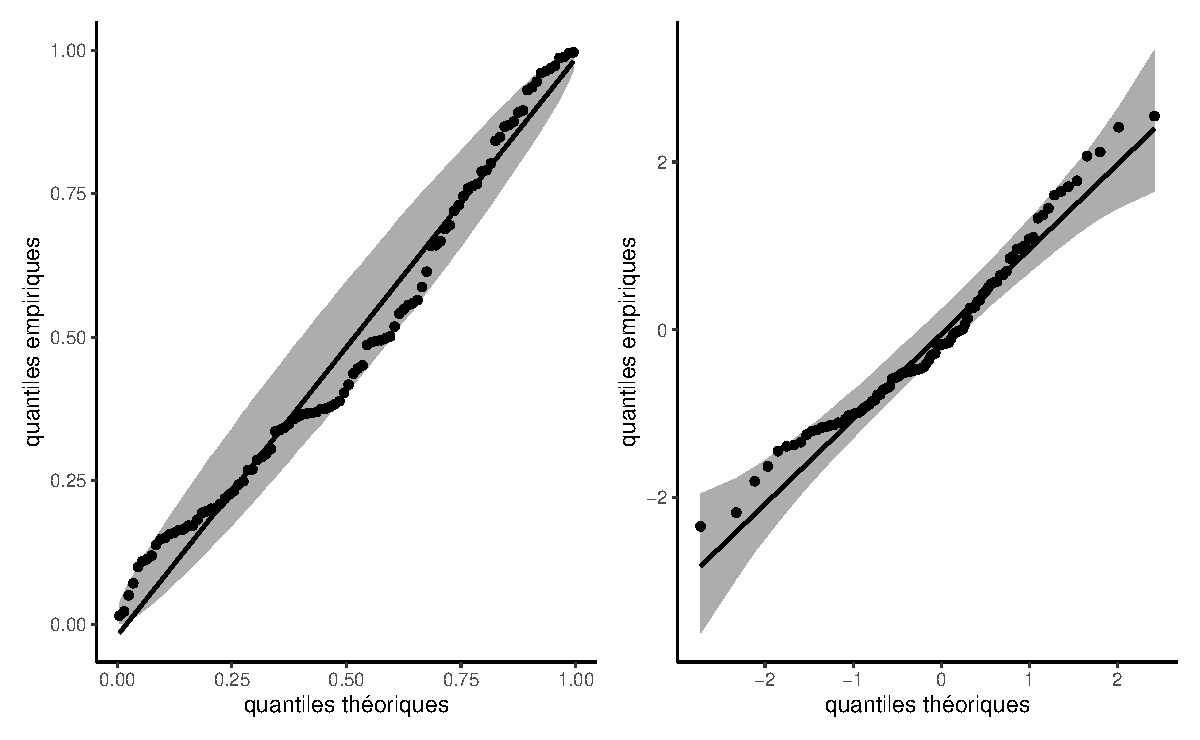
\includegraphics[width=0.85\textwidth,height=\textheight]{introduction_files/figure-pdf/fig-diagrammeqq2-1.pdf}

}

\caption{\label{fig-diagrammeqq2}Diagramme probabilité-probabilité
(gauche) et quantile-quantile normal (droite)}

\end{figure}%

Même si on connaissait exactement la loi aléatoire des données, la
variabilité intrinsèque à l'échantillon fait en sorte que des déviations
qui semblent significatives et anormales à l'oeil de l'analyste sont en
fait compatibles avec le modèle: un simple estimé ponctuel sans mesure
d'incertitude ne permet donc pas facilement de voir ce qui est plausible
ou pas. On va donc idéalement ajouter un intervalle de confiance
(approximatif) ponctuel ou conjoint au diagramme.

Pour obtenir l'intervalle de confiance approximatif, la méthode la plus
simple est par simulation, en répétant \(B\) fois les étapes suivantes

\begin{enumerate}
\def\labelenumi{\arabic{enumi}.}
\tightlist
\item
  simuler un échantillon \(\{Y^{(b)}_{i}\} (i=1,\ldots, n)\) du modèle
  \(\widehat{F}\)
\item
  estimer les paramètres du modèle \(F\) pour obtenir
  \(\widehat{F}_{(b)}\)
\item
  calculer et stocker les positions
  \(\widehat{F}^{-1}_{(b)}\{i/(n+1)\}\).
\end{enumerate}

Le résultat de cette opération sera une matrice \(n \times B\) de
données simulées; on obtient un intervalle de confiance symmétrique en
conservant le quantile \(\alpha/2\) et \(1-\alpha/2\) de chaque ligne.
Le nombre de simulation \(B\) devrait être large (typiquement 999 ou
davantage) et être choisi de manière à ce que \(B/\alpha\) soit un
entier.

Pour l'intervalle de confiance ponctuel, chaque valeur représente une
statistique et donc individuellement, la probabilité qu'une statistique
d'ordre sorte de l'intervalle de confiance est \(\alpha\). En revanche,
les statistiques d'ordres ne sont pas indépendantes et sont qui est plus
ordonnées, ce qui fait qu'un point hors de l'intervalle risque de n'être
pas isolé. Les intervalles présentés dans la
Figure~\ref{fig-diagrammeqq2} sont donc ponctuels. La variabilité des
statistiques d'ordre uniformes est plus grande autour de 1/2, mais
celles des variables transformées dépend de \(F\).

L'interprétation d'un diagramme quantile-quantile nécessite une bonne
dose de pratique et de l'expérience:
\href{https://stats.stackexchange.com/questions/101274/how-to-interpret-a-qq-plot/101290\#101290}{cette
publication par \emph{Glen\_b} sur StackOverflow} résume bien ce qu'on
peut détecter ou pas en lisant le diagramme.

\section{Loi des grands nombres}\label{loi-grands-nombres}

Un estimateur est dit \textbf{convergent} si la valeur obtenue à mesure
que la taille de l'échantillon augmente s'approche de la vraie valeur
que l'on cherche à estimer. Mathématiquement parlant, un estimateur est
dit convergent s'il converge en probabilité, ou
\(\hat{\theta} \stackrel{\mathsf{Pr}}{\to} \theta\): en langage commun,
la probabilité que la différence entre \(\hat{\theta}\) et \(\theta\)
diffèrent est négligeable quand \(n\) est grand.

La condition \emph{a minima} pour le choix d'un estimateur est donc la
convergence: plus on récolte d'information, plus notre estimateur
devrait s'approcher de la valeur qu'on tente d'estimer.

La loi des grands nombres établit que la moyenne empirique de \(n\)
observations indépendantes de même espérance, \(\overline{Y}_n\), tend
vers l'espérance commune des variables \(\mu\), où
\(\overline{Y}_n \rightarrow \mu\). En gros, ce résultat nous dit que
l'on réussit à approximer de mieux en mieux la quantité d'intérêt quand
la taille de l'échantillon (et donc la quantité d'information disponible
sur le paramètre) augmente. La loi des grands nombres est très utile
dans les expériences Monte Carlo: on peut ainsi approximer par
simulation la moyenne d'une fonction \(g(x)\) de variables aléatoires en
simulant de façon répétée des variables \(Y\) indépendantes et
identiquement distribuées et en prenant la moyenne empirique
\(n^{-1} \sum_{i=1}^n g(Y_i)\).

Si la loi des grands nombres nous renseigne sur le comportement limite
ponctuel, il ne nous donne aucune information sur la variabilité de
notre estimé de la moyenne et la vitesse à laquelle on s'approche de la
vraie valeur du paramètre.

\section{Théorème central limite}\label{TCL}

Le théorème central limite dit que, pour un échantillon aléatoire de
taille \(n\) dont les observations sont indépendantes et tirées d'une
loi quelconque d'espérance \(\mu\) et de variance finie \(\sigma^2\),
alors la moyenne empirique tend non seulement vers \(\mu\), mais à une
vitesse précise:

\begin{itemize}
\tightlist
\item
  l'estimateur \(\overline{Y}\) sera centré autour de \(\mu\),
\item
  l'erreur-type sera de \(\sigma/\sqrt{n}\); le taux de convergence est
  donc de \(\sqrt{n}\). Ainsi, pour un échantillon de taille 100,
  l'erreur-type de la moyenne empirique sera 10 fois moindre que
  l'écart-type de la variable aléatoire sous-jacente.
\item
  la loi approximative de la moyenne \(\overline{Y}\) sera normale.
\end{itemize}

Mathématiquement, le théorème central limite dicte que
\(\sqrt{n}(\overline{Y}-\mu) \stackrel{\mathrm{d}}{\rightarrow} \mathsf{normale}(0, \sigma^2)\).
Si \(n\) est grand (typiquement supérieur à \(30\), mais cette règle
dépend de la loi sous-jacente de \(Y\)), alors
\(\overline{Y} \stackrel{\cdot}{\sim} \mathsf{normale}(\mu, \sigma^2/n)\).

Comment interpréter ce résultat? On considère comme exemple le temps de
trajet moyen de trains à haute vitesse AVE entre Madrid et Barcelone
opérés par la Renfe.

\begin{figure}[ht!]

\centering{

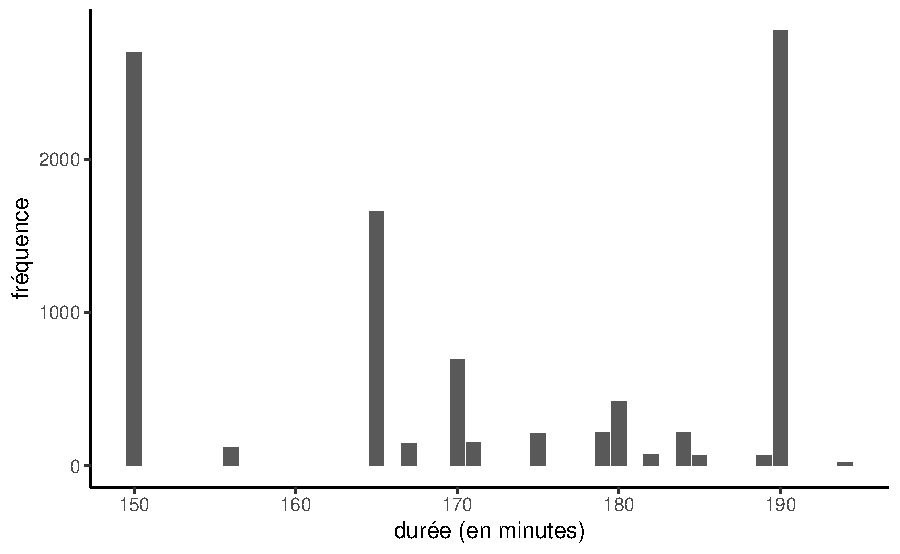
\includegraphics[width=0.85\textwidth,height=\textheight]{introduction_files/figure-pdf/fig-renfeclt-1.pdf}

}

\caption{\label{fig-renfeclt}Distribution empirique des temps de trajet
en trains à grande vitesse.}

\end{figure}%

Une analyse exploratoire indique que la durée du trajet de la base de
données est celle affichée sur le billet (et non le temps réel du
parcours). Ainsi, il n'y a ainsi que 15 valeurs possibles. Le temps
affiché moyen pour le parcours, estimé sur la base de 9603 observations,
est de 170 minutes et 41 secondes. La Figure~\ref{fig-renfeclt} montre
la distribution empirique des données.

Considérons maintenant des échantillons de taille \(n=10\). Dans notre
premier échantillon aléatoire, la durée moyenne affichée est 169.3
minutes, elle est de 167 minutes dans le deuxième, de 157.9 dans le
troisième, et ainsi de suite.

\begin{figure}[ht!]

\centering{

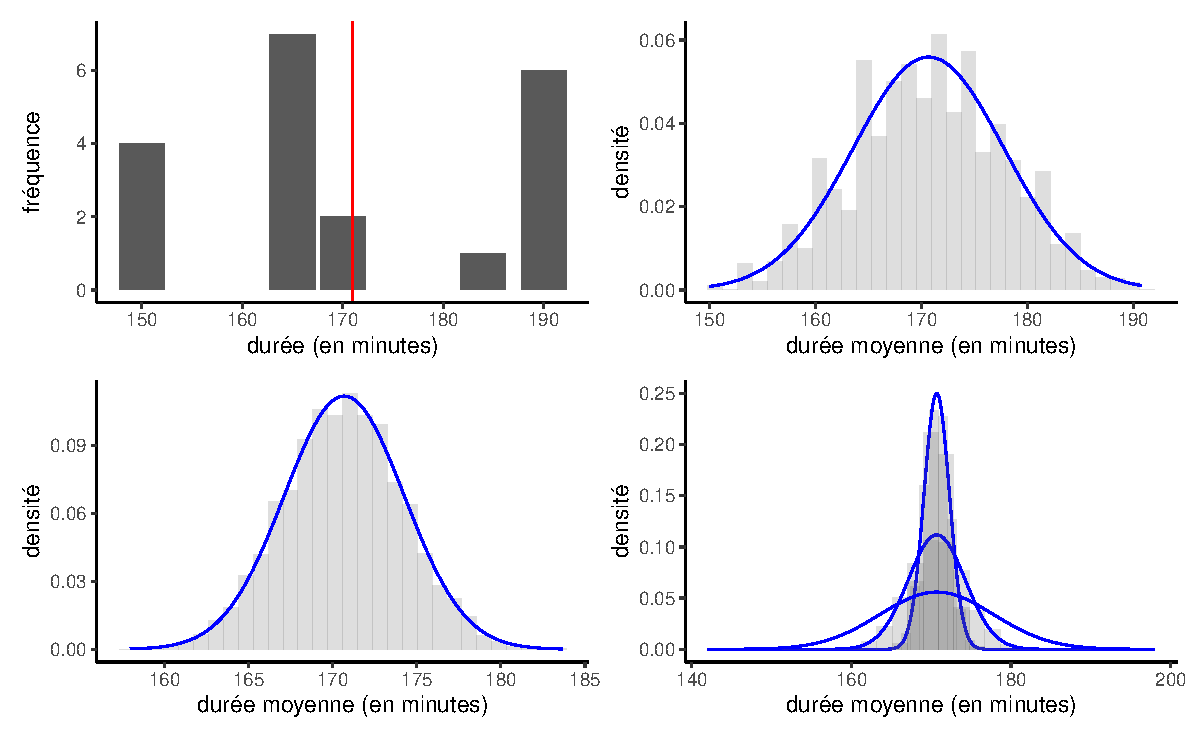
\includegraphics[width=0.9\textwidth,height=\textheight]{introduction_files/figure-pdf/fig-renfemeanCLT-1.pdf}

}

\caption{\label{fig-renfemeanCLT}Représentation graphique du théorème
central limite: échantillon aléatoire de 20 observations avec leur
moyenne empirique (trait vertical rouge) (en haut à gauche). Les trois
autres panneaux montrent les histogrammes des moyennes empiriques
d'échantillons répétés de taille 5 (en haut à droite), 20 (en bas à
gauche) et les histogrammes pour \(n=5, 20, 100\) (en bas à droite) avec
courbe de densité de l'approximation normale fournie par le théorème
central limite.}

\end{figure}%

Supposons qu'on tire \(B=1000\) échantillons différents, chacun de
taille \(n=5\), de notre ensemble, et qu'on calcule la moyenne de chacun
d'entre eux. Le graphique supérieur droit de la
Figure~\ref{fig-renfemeanCLT} montre un de ces 1000 échantillons
aléatoire de taille \(n=20\) tiré de notre base de données. Les autres
graphiques de la Figure~\ref{fig-renfemeanCLT} illustrent l'effet de
l'augmentation de la taille de l'échantillon: si l'approximation normale
est approximative avec \(n=5\), la distribution des moyennes est
virtuellement identique à partir de \(n=20\). Plus la moyenne est
calculée à partir d'un grand échantillon (c'est-à-dire, plus \(n\)
augmente), plus la qualité de l'approximation normale est meilleure et
plus la courbe se concentre autour de la vraie moyenne; malgré le fait
que nos données sont discrètes, la distribution des moyennes est
approximativement normale.

On a considéré une seule loi aléatoire inspirée de l'exemple, mais vous
pouvez vous amuser à regarder l'effet de la distribution sous-jacent et
de la taille de l'échantillon nécessaire pour que l'effet du théorème
central limite prenne effet: il suffit pour cela de simulant des
observations d'une loi quelconque de variance finie, en utilisant par
exemple cette
\href{http://195.134.76.37/applets/AppletCentralLimit/Appl_CentralLimit2.html}{applette}.

Les statistiques de test qui découlent d'une moyenne centrée-réduite (ou
d'une quantité équivalente pour laquelle un théorème central limite
s'applique) ont souvent une loi nulle standard normale, du moins
asymptotiquement (quand \(n\) est grand, typiquement \(n>30\) est
suffisant). C'est ce qui garantie la validité de notre inférence!

\bookmarksetup{startatroot}

\chapter{Inférence statistique}\label{inference}

Dans la plupart des domaines scientifiques, les donnéese empiriques
issues d'expériences contribuent à l'édification de la science. Afin de
tirer des conclusions en faveur ou à l'encontre d'une théorie, les
chercheurs se tournent (souvent à contrecoeur) vers la statistique. Cela
a conduit à la prédominance de l'utilisation du cadre des tests
statistiques et à la prépondérance des valeurs-\(p\) dans les articles
scientifiques, souvent employées de manière abusive ou fautive dans les
articles de journaux. La falsification d'une hypothèse nulle n'est pas
suffisante pour fournir des résultats substantiels pour une théorie.

Comme les cours d'introduction aux statistiques présentent généralement
des tests d'hypothèses sans accorder beaucoup d'attention aux principes
de construction sous-jacents de ces procédures, les utilisateurs ont
souvent une vision réductrice des statistiques. Plusieurs voient les
statistiques comme un catalogue de procédures pré-établies. Pour faire
une analogie culinaire, les utilisateurs se concentrent sur
l'apprentissage en vase clos des recettes plutôt que d'essayer de
comprendre les bases de la cuisine et de faire des liens. Ce chapitre se
concentre sur la compréhension des concepts-clés liées aux tests.

\begin{tcolorbox}[enhanced jigsaw, colbacktitle=quarto-callout-important-color!10!white, title=\textcolor{quarto-callout-important-color}{\faExclamation}\hspace{0.5em}{Objectifs d'apprentissage}, leftrule=.75mm, opacityback=0, colframe=quarto-callout-important-color-frame, breakable, toprule=.15mm, coltitle=black, toptitle=1mm, colback=white, bottomrule=.15mm, bottomtitle=1mm, titlerule=0mm, arc=.35mm, rightrule=.15mm, left=2mm, opacitybacktitle=0.6]

\begin{itemize}
\tightlist
\item
  Comprendre le rôle de l'incertitude dans la prise de décision.
\item
  Comprendre l'importance du rapport signal/bruit en tant que preuve.
\item
  Connaître les ingrédients de base des tests d'hypothèse et être
  capable de formuler et d'identifier correctement ces composants dans
  un article scientifique
\item
  Interpréter correctement les valeurs-\(p\) et les intervalles de
  confiance pour un paramètre.
\end{itemize}

\end{tcolorbox}

Avant d'entamer une collecte de données pour une expérience, il est
nécessaire de formuler une question de recherche. En général, cette
hypothèse spécifie les différences potentielles entre les
caractéristiques de la population dues à une intervention (un
traitement) que le chercheur souhaite quantifier. C'est à cette étape
que les chercheurs décident de la taille de l'échantillon, du choix de
la variable de réponse et de la méthode de mesure, qu'ils rédigent le
plan de l'étude, etc.

Il est important de noter que la plupart des questions de recherche ne
peuvent être résolues à l'aide d'outils simples. Les chercheurs qui
souhaitent mener une recherche méthodologique innovante devraient
contacter des experts et consulter des statisticien(ne)s \textbf{avant}
de collecter leurs données afin d'obtenir des informations sur la
meilleure façon de procéder pour ce qu'ils ont en tête, afin d'éviter le
risque d'affirmations trompeuses basées sur une analyse ou une collecte
de données incorrectes.

\begin{figure}[ht!]

\centering{

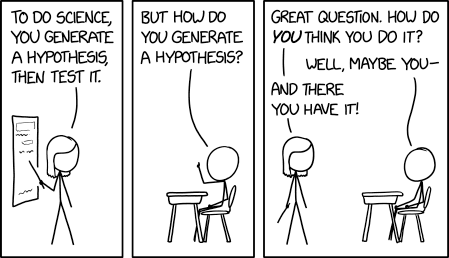
\includegraphics[width=0.6\textwidth,height=\textheight]{images/xkcd2569_hypothesis_generation.png}

}

\caption{\label{fig-xkcd2569}Bande dessinée xkcd
\href{https://xkcd.com/2569/}{2569 (Hypothesis generation) par Randall
Munroe}. Texte alternatif: Frazzled scientists are requesting that
everyone please stop generating hypotheses for a little bit while they
work through the backlog. Bande réimprimée sous license
\href{https://creativecommons.org/licenses/by-nc/2.5/}{CC BY-NC 2.5}.}

\end{figure}%

\section{Variabilité
échantillonale}\label{variabilituxe9-uxe9chantillonale}

Un chercheur s'intéressera à l'estimation de certaines caractéristiques
de la population à partir d'une base de données. Nous pouvons
caractériser l'ensemble de toutes les valeurs potentielles que leurs
mesures peuvent prendre, ainsi que leur fréquence, au moyen d'une loi
d'une variable aléatoire.

L'objectif de cette section est d'illustrer le fait que nous ne pouvons
pas simplement utiliser les différences brutes entre les groupes pour
effectuer des comparaisons significatives: en raison de la variabilité
due à l'échantillonnage, les échantillons seront semblables même s'ils
sont générés de la même manière, mais il y aura toujours des différences
entre les statistiques récapitulatives calculées sur des échantillons
différents. Ces différences ont tendance à s'atténuer (ou à augmenter)
au fur et à mesure que l'on collecte davantage d'observations. Plus nous
recueillons de données (et donc d'informations) sur notre cible, plus le
portrait devient précis. C'est somme toute ce qui nous permet de tirer
des conclusions mais, pour ce faire, nous devons d'abord déterminer ce
qui est probable ou plausible et donc le fruit du hsard, de ce qui n'est
pas ou peu susceptible de se produire.

Nous appelons \textbf{statistiques} les résumés numériques des données.
Il est important de faire la distinction entre les procédures ou
formules et leurs valeurs numériques. Un \textbf{estimateur} est une
règle ou une formule utilisée pour calculer une estimation d'un
paramètre ou d'une quantité d'intérêt sur la base de données observées
(comme une recette de gâteau). Une fois que nous disposons de données
observées, nous pouvons calculer la moyenne de l'échantillon,
c'est-à-dire que nous disposons d'une estimation --- d'une valeur réelle
(le gâteau), qui est une réalisation unique et non aléatoire. En
d'autres termes,

\begin{itemize}
\tightlist
\item
  un estimand est notre cible conceptuelle, comme la caractéristique de
  la population qui nous intéresse (la moyenne de la population).
\item
  un estimateur est la procédure ou la formule qui nous indique comment
  transformer les données de l'échantillon en un résumé numérique qui
  est une approximation de notre cible.
\item
  une estimation (ou un estimé) est un nombre, la valeur numérique
  obtenue lorsque nous appliquons la formule à un échantillon en
  praticulier.
\end{itemize}

\begin{figure}[ht!]

\begin{minipage}{0.33\linewidth}

\centering{


\includegraphics[width=0.85\textwidth,height=\textheight]{images/estimand.jpg}

}

\subcaption{\label{fig-cake-1}Estimand}

\end{minipage}%
%
\begin{minipage}{0.33\linewidth}

\centering{

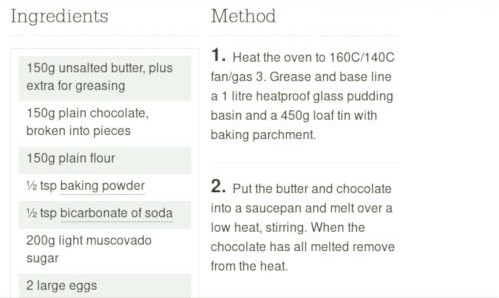
\includegraphics[width=0.85\textwidth,height=\textheight]{images/estimator.jpg}

}

\subcaption{\label{fig-cake-2}Estimateur}

\end{minipage}%
%
\begin{minipage}{0.33\linewidth}

\centering{


\includegraphics[width=0.85\textwidth,height=\textheight]{images/estimate.jpg}

}

\subcaption{\label{fig-cake-3}Estimé}

\end{minipage}%

\caption{\label{fig-cake}Les concepts
d'\href{https://www.flickr.com/photos/darkdwarf/16563489881}{estimand}
(gauche), estimateur (milieu) et
\href{https://www.flickr.com/photos/bensutherland/14685548773}{estimaté}
(droite), illustrés à l'aide de gâteau, une variation d'un idée
originale de Simon Grund. Les photos de gâteau sont partagées sous
licence \href{https://creativecommons.org/licenses/by-nc/2.0/}{CC BY-NC
2.0}.}

\end{figure}%

Par exemple, si l'estimand est l'espérance de la population \(\mu,\)
l'estimateur sera la moyenne arithmétique, soit la somme des éléments de
l'échantillon aléatoire divisé par la taille de l'échantillon, ou,
\(\overline{Y}=(Y_1 + \cdots + Y_n)/n.\) L'estimé sera une valeur
numérique, disons 4.3.

Parce que les intrants de l'estimateur sont aléatoires, la sortie l'est
également et varie d'un échantillon à l'autre. Autrement dit, même si on
répète une recette, on n'obtient pas le même résultat à chaque coup,
comme le montre si bien la Figure~\ref{fig-xkcd605}.

\begin{figure}[ht!]

\centering{

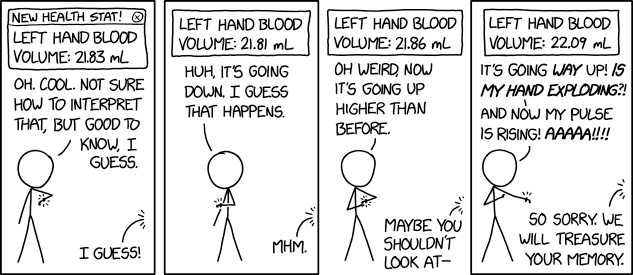
\includegraphics[width=0.7\textwidth,height=\textheight]{images/xkcd2581_health_stats.png}

}

\caption{\label{fig-xkcd605}Bande dessinée xkcd
\href{https://xkcd.com/2581/}{2581 (Health Stats) par Randall Munroe}.
Texte alternatif: You will live on forever in our hearts, pushing a
little extra blood toward our left hands now and then to give them a
squeeze. Bande réimprimée sous license
\href{https://creativecommons.org/licenses/by-nc/2.5/}{CC BY-NC 2.5}.}

\end{figure}%

Pour illustrer ce point, Figure~\ref{fig-samplevar} montre cinq
échantillons aléatoires simples de taille \(n=10\) tirés d'une
population hypothétique de moyenne théorique \(\mu\) et d'écart-type
\(\sigma,\) ainsi que leur moyenne d'échantillon \(\overline{y}.\) En
raison de la variabilité échantillonnale, les moyennes des sous-groupes
sont différentes même si elles proviennent de la même population. Vous
pouvez considérer la variabilité d'échantillonnage comme du bruit: notre
objectif est d'extraire le signal (typiquement les différences de
moyennes) tout en tenant compte du bruit de fond.

\begin{figure}[ht!]

\centering{

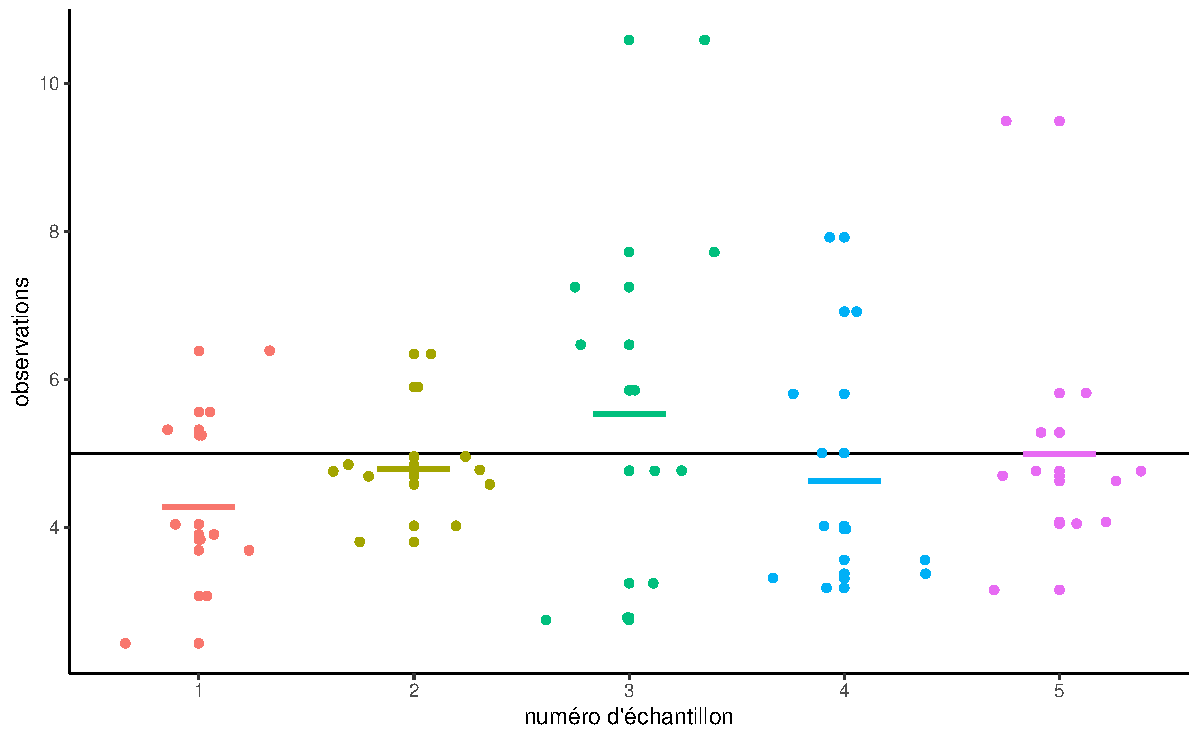
\includegraphics[width=0.85\textwidth,height=\textheight]{inference_files/figure-pdf/fig-samplevar-1.pdf}

}

\caption{\label{fig-samplevar}Cinq échantillons de taille \(n=10\) tirés
d'une population commune de moyenne \(\mu\) (ligne horizontale). Les
segments colorés représentent les moyennes empiriques de chaque groupe.}

\end{figure}%

L'oeil avisé pourra remarquer que les moyennes des cinq échantillons
(segments horizontaux colorés) sont moins dispersées autour de la ligne
horizontale noire représentant la moyenne de la population \(\mu\) que
ne le sont les observations. Il s'agit là d'un principe fondamental de
la statistique: l'information s'accumule au fur et à mesure que l'on
obtient plus de données.

Les valeurs de la moyenne de l'échantillon ne donnent pas une image
complète et l'étude des différences de moyenne (entre les groupes ou par
rapport à une valeur de référence postulée) n'est pas suffisante pour
tirer des conclusions. Dans la plupart des cas, rien ne garantit que la
moyenne de l'échantillon sera égale à sa valeur réelle, car elle varie
d'un échantillon à l'autre: la seule garantie que nous ayons est qu'elle
sera en moyenne égale à la moyenne de la population dans des
échantillons répétés. Selon le choix de la mesure et la variabilité de
la population, il peut y avoir des différences considérables d'une
observation à l'autre, ce qui signifie que la différence observée peut
être un coup de chance.

Pour avoir une idée du degré de certitude d'une chose, nous devons
considérer la variabilité d'une observation \(Y_i.\) Cette variance
d'une observation tirée de la population est typiquement notée
\(\sigma^2\) et sa racine carrée, l'écart-type, par \(\sigma.\)

L'écart-type \emph{d'une statistique} est appelé \textbf{erreur-type};
il ne doit pas être confondu avec l'écart-type \(\sigma\) de la
population dont sont tirées les observations de l'échantillon
\(Y_1, \ldots, Y_n.\) L'écart-type et l'erreur-type sont exprimés dans
les mêmes unités que les données et sont donc plus faciles à interpréter
que la variance. L'erreur-type étant fonction de la taille de
l'échantillon, il est d'usage de rapporter plutôt l'écart-type dans les
rapports.

\begin{example}[Proportion échantillonale et tirages
uniformes]\protect\hypertarget{exm-samppropunif}{}\label{exm-samppropunif}

Pour illustrer le concept de variabilité échantillonnale, nous suivons
l'exemple de {[}Matthew Crump{]}
(https://www.crumplab.com/statistics/foundations-for-inference.html) et
considérons des échantillons provenant d'une distribution uniforme sur
\(\{1, 2, \ldots, 10\}\): chaque entier de cet intervalle a la même
probabilité d'être tiré.

\begin{figure}[ht!]

\centering{

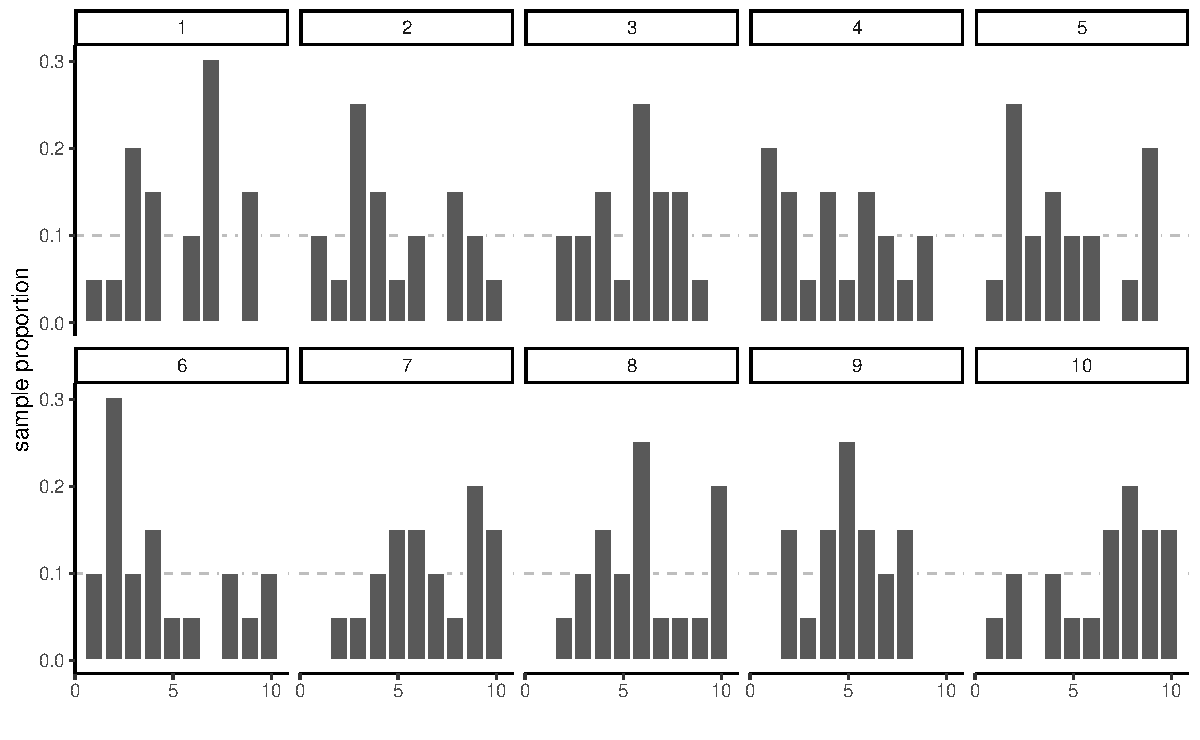
\includegraphics[width=0.85\textwidth,height=\textheight]{inference_files/figure-pdf/fig-unifsamp1-1.pdf}

}

\caption{\label{fig-unifsamp1}Histogrammes de 10 échantillons aléatoires
de taille \(n=20\) de loi uniforme discrète.}

\end{figure}%

Même s'ils sont tirés de la même population, les 10 échantillons de
Figure~\ref{fig-unifsamp1} sont très différents. La seule chose en jeu
ici est la variabilité de l'échantillon: puisqu'il y a \(n=20\)
d'observations au total, il devrait y avoir en moyenne 10\% des
observations dans chacun des 10 bacs, mais certains bacs sont vides et
d'autres ont plus d'effectifs que prévu. Cette fluctuation est le fruit
du hasard.

Comment pouvons-nous donc déterminer si ce que nous voyons est
compatible avec le modèle qui, selon nous, a généré les données ? Il
suffit de collecter davantage d'observations: la hauteur de la barre est
la proportion de l'échantillon, une moyenne de valeurs 0/1, où la valeur
`un' indique que l'observation se trouve dans la case, et `zéro' dans le
cas contraire.

Considérons maintenant ce qui se passe lorsque nous augmentons la taille
de l'échantillon: le panneau supérieur de Figure~\ref{fig-uniformsamp2}
montre des échantillons uniformes pour une taille d'échantillon
croissante. Le diagramme à bande ressemble de plus en plus à la
véritable distribution sous-jacente (fonction de masse constante, donc
chaque case ayant la même fréquence) à mesure que la taille de
l'échantillon augmente. La distribution des points de l'échantillon est
presque indiscernable de la distribution théorique (ligne droite)
lorsque \(n=10 000.\)\footnote{La formule montre que l'erreur standard
  diminue d'un facteur 10 chaque fois que la taille de l'échantillon
  augmente d'un facteur 100.}. Le panneau du bas, en revanche, ne
provient pas d'une distribution uniforme. Plus l'échantillon grossit,
plus l'approximation de la fonction de masse se rapproche de la vraie
valeur. Nous n'aurions pas pu remarquer cette différence dans les deux
premiers graphiques, car la variabilité de l'échantillonnage est trop
importante; là, le manque de données dans certaines cases pourrait être
un obstacle à l'obtention d'une distribution uniforme.

\begin{figure}[ht!]

\centering{

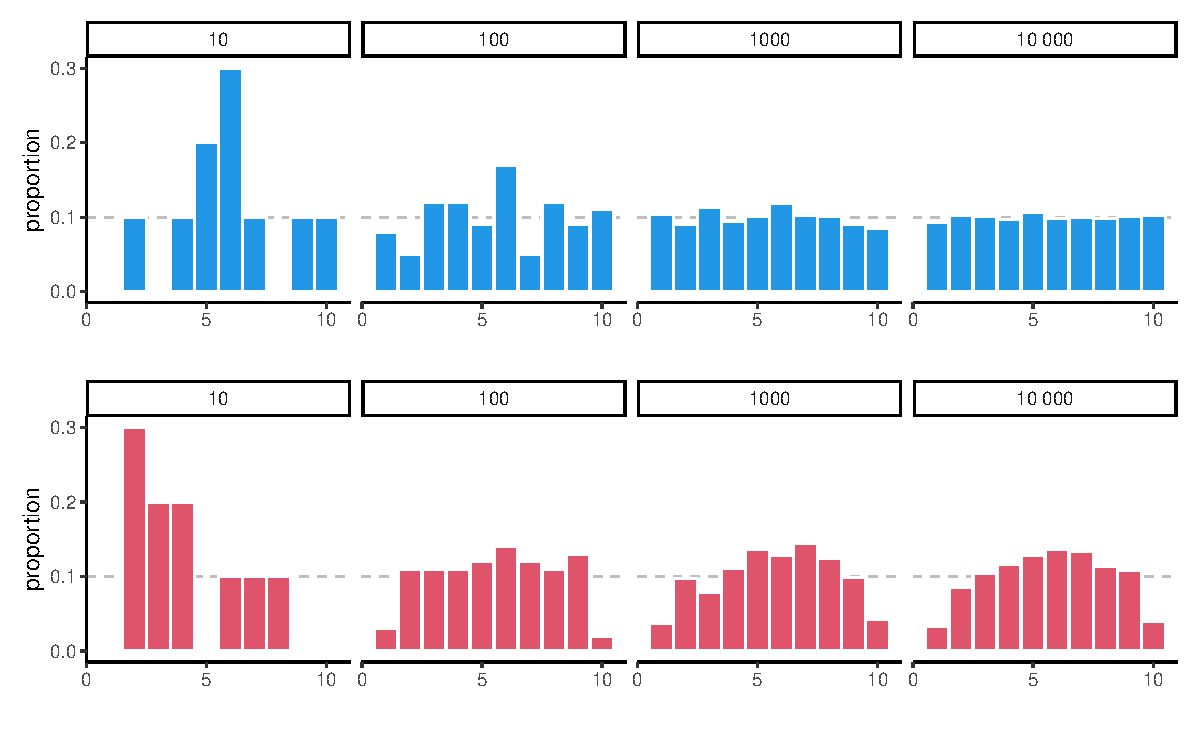
\includegraphics[width=0.85\textwidth,height=\textheight]{inference_files/figure-pdf/fig-uniformsamp2-1.pdf}

}

\caption{\label{fig-uniformsamp2}Histogrammes de données tirées d'une
loi uniforme (haut) et d'une loi non-uniforme (bas) pour des tailles
d'échantillons de 10, 100, 1000 and 10 000 (de gauche à droite).}

\end{figure}%

\end{example}

\section{Tests d'hypothèse}\label{tests}

Un test d'hypothèse statistique est une façon d'évaluer la preuve
statistique provenant d'un échantillon afin de faire une décision quant
à la population sous-jacente. Les étapes principales sont:

\begin{itemize}
\tightlist
\item
  définir les paramètres du modèle,
\item
  formuler les hypothèses alternative et nulle,
\item
  choisir et calculer la statistique de test,
\item
  déterminer son comportement sous \(\mathscr{H}_0\) (loi nulle),
\item
  calculer la valeur-\emph{p},
\item
  conclure dans le contexte du problème (rejeter ou ne pas rejeter
  \(\mathscr{H}_0\)).
\end{itemize}

Mon approche privilégiée pour présenter les tests d'hypothèse est de
faire un parallèle avec un procès pour meurtre où vous êtes nommé juré.

\begin{itemize}
\tightlist
\item
  Le juge vous demande de choisir entre deux hypothèses mutuellement
  exclusives, coupable ou non-coupable, sur la base des preuves
  présentées.
\item
  Votre postulat de départ repose sur la présomption d'innocence: vous
  condamnerez uniquement le suspect si la preuve est accablante. Cela
  permet d'éviter les erreurs judiciaires. L'hypothèse nulle
  \(\mathscr{H}_0\) est donc \emph{non-coupable}, et l'hypothèse
  alternative \(\mathscr{H}_a\) est coupable. En cas de doute
  raisonnable, vous émettrez un verdict de non-culpabilité.
\item
  La choix de la statistique de test représente la preuve. Plus la
  preuve est accablante, plus grande est la chance d'un verdict de
  culpabilité --- le procureur a donc tout intérêt à bien choisir les
  faits présentés en cour. Le choix de la statistique devrait donc
  idéalement maximiser la preuve pour appuyer le postulat de culpabilité
  le mieux possible (ce choix reflète la \textbf{puissance} du test).
\item
  En qualité de juré, vous analysez la preuve à partir de la
  jurisprudence et de l'avis d'expert pour vous assurer que les faits ne
  relèvent pas du hasard. Pour le test d'hypothèse, ce rôle est tenu par
  la loi sous \(\mathscr{H}_0\): si la personne était innocente, est-ce
  que les preuves présentées tiendraient la route? des traces d'ADN
  auront davantage de poids que des ouï-dire (la pièce de théâtre
  \emph{Douze hommes en colère} de Reginald Rose présente un bel exemple
  de procès où un des juré émet un doute raisonnable et convainc un à un
  les autres membres du jury de prononcer un verdict de
  non-culpabilité).
\item
  Vous émettez un verdict, à savoir une décision binaire, où l'accusé
  est déclaré soit non-coupable, soit coupable. Si vous avez une
  valeur-\emph{p}, disons \(P,\) pour votre statistique de test et que
  vous effectuez ce dernier à niveau \(\alpha,\) la règle de décision
  revient à rejeter \(\mathscr{H}_0\) si \(P < \alpha.\)
\end{itemize}

On s'attarde davantage sur ces définitions heuristiques et le
vocabulaire employé pour parler de tests d'hypothèse.

\section{Hypothèse}\label{hypothuxe8se}

Dans les test statistique il y a toujours deux hypothèse: l'hypothèse
nulle (\(\mathscr{H}_{0}\)) et l'hypothèse alternative
(\(\mathscr{H}_a\)). Habituellement, l'hypothèse nulle est le « statu
quo » et l'alternative est l'hypothèse que l'on cherche à démontrer. On
se fait l'avocat du Diable en défendant l'hypothèse nulle et en
analysant toutes les preuves sous l'angle: « est-ce que les données
entrent en contradiction avec \(\mathscr{H}_0\)? ». Un test d'hypothèse
statistique nous permet de décider si nos données nous fournissent assez
de preuves pour rejeter \(\mathscr{H}_0\) en faveur de
\(\mathscr{H}_a,\) selon un risque d'erreur spécifié.

Généralement, les tests d'hypothèses sont exprimés en fonction de
paramètres (de valeurs inconnues) du modèle sous-jacent, par ex.
\(\theta.\) Un test d'hypothèse bilatéral concernant un paramètre
scalaire \(\theta\) s'exprimerait la forme suivante: \begin{align*}
\mathscr{H}_0: \theta=\theta_0 \qquad \text{versus} \qquad \mathscr{H}_a:\theta \neq \theta_0.
\end{align*} Ces hypothèses permettent de tester si \(\theta\) est égal
à une valeur numérique précise \(\theta_0.\)

Par exemple, pour un test bilatéral concernant le paramètre d'un modèle
de régression \(\beta_j\) associé à une variable explicative d'intérêt
\(\mathrm{X}_j,\) les hypothèses sont \begin{align*}
\mathscr{H}_0: \beta_j=\beta_j^0 \qquad \text{versus} \qquad \mathscr{H}_a:\beta_j \neq \beta_j^0,
\end{align*} où \(\beta_j^0\) est une valeur précise qui est reliée à la
question de recherche. Par exemple, si \(\beta_j^0=0\) la question de
recherche sous-jacente est: est-ce que la covariable \(\mathrm{X}_j\)
impacte la variable réponse d'intérêt \(Y\) une fois l'effet des autres
variables pris en compte?

Il est possible d'imposer une direction dans les tests en considérant
une hypothèse alternative de la forme
\(\mathscr{H}_a: \theta > \theta_0\) ou
\(\mathscr{H}_a: \theta < \theta_0.\)

\section{Statistique de test}\label{statistique-de-test}

Une statistique de test \(T\) est une fonction des données qui résume
l'information contenue dans les données pour \(\theta.\) La forme de la
statistique de test est choisie de façon à ce que son comportement sous
\(\mathscr{H}_0,\) c'est-à-dire l'ensemble des valeurs que prend \(T\)
si \(\mathscr{H}_0\) est vraie et leur probabilité relative, soit connu.
En effet, \(T\) est une variable aléatoire et sa valeur va changer selon
l'échantillon. La \textbf{loi nulle} de la statistique de test nous
permet de déterminer quelles valeurs de \(T\) sont plausibles si
\(\mathscr{H}_0\) est vraie. Plusieurs statistiques que l'on couvrira
dans ce cours sont des \textbf{statistiques de Wald}, de la forme
\begin{align*}
T = \frac{\widehat{\theta} - \theta_0}{\mathrm{se}(\widehat{\theta})}
\end{align*} où \(\widehat{\theta}\) est l'estimateur du paramètre
\(\theta,\) \(\theta_0\) la valeur numérique postulée (par ex., zéro) et
\(\mathrm{se}(\widehat{\theta})\) est l'estimateur de l'écart-type de
\(\widehat{\theta}.\)

Par exemple, pour une hypothèse sur la moyenne d'une population de la
forme \begin{align*}
\mathscr{H}_0: \mu=0, \qquad  \mathscr{H}_a:\mu \neq 0,
\end{align*} la statistique de test de Wald est \begin{align*}
T &= \frac{\overline{X}-0}{S_n/\sqrt{n}}
\end{align*} où \(\overline{X}\) est la moyenne de l'échantillon
\(X_1, \ldots, X_n,\) \begin{align*}
\overline{X} &= \frac{1}{n} \sum_{i=1}^n X_i = \frac{X_1+ \cdots + X_n}{n}
\end{align*} et l'erreur-type de la moyenne \(\overline{X}\) est
\(S_n/\sqrt{n}\); l'écart-type \(S_n\) est un estimateur de \(\sigma,\)
où \begin{align*}
S^2_n &= \frac{1}{n-1} \sum_{i=1}^n (X_i-\overline{X})^2.
\end{align*}

\section{\texorpdfstring{Loi nulle et
valeur-\emph{p}}{Loi nulle et valeur-p}}\label{loi-nulle-et-valeur-p}

La \textbf{valeur-\emph{p}} nous permet de déterminer si la valeur
observée de la statistique de test \(T\) est plausible sous
\(\mathscr{H}_0.\) Plus précisément, la valeur-\emph{p} est la
probabilité, si \(\mathscr{H}_0\) est vraie, que la statistique de test
soit égale or plus extrême à ce qu'on observe. Supposons qu'on a un
échantillon \(X_1, \ldots, X_n\) et qu'on observe une valeur de la
statistique de test de \(T=t.\) Pour un test d'hypothèse bilatéral
\(\mathscr{H}_0:\theta=\theta_0\)
vs.~\(\mathscr{H}_a:\theta \neq \theta_0,\) la valeur-\emph{p} est
\(\Pr{\!}_0(|T| \geq |t|).\) Si la distribution de \(T\) est symétrique
autour de zéro, la valeur-\emph{p} vaut \begin{align*}
p = 2 \times \Pr{\!}_0(T \geq |t|).
\end{align*}

La Figure~\ref{fig-power-plots} montre la loi des valeurs-\(p\) sous
deux scénarios: à gauche, une loi nulle et à droite, une loi
alternative. La probabilité de rejetter \(\mathscr{H}_0\) est obtenue en
calculant l'aire sous la courbe sous la courbe de densité et
\(\alpha=0.1.\) Sous l'hypothèse nulle, le modèle est calibré et la loi
des valeurs-\(p\) est uniforme (un rectangle de hauteur 1), ce qui veut
dire que toutes les valeurs sont également plausibles. Sous
l'alternative, l'obtention de petites valeurs\(-\)p est plus plausible.

\begin{figure}[ht!]

\centering{

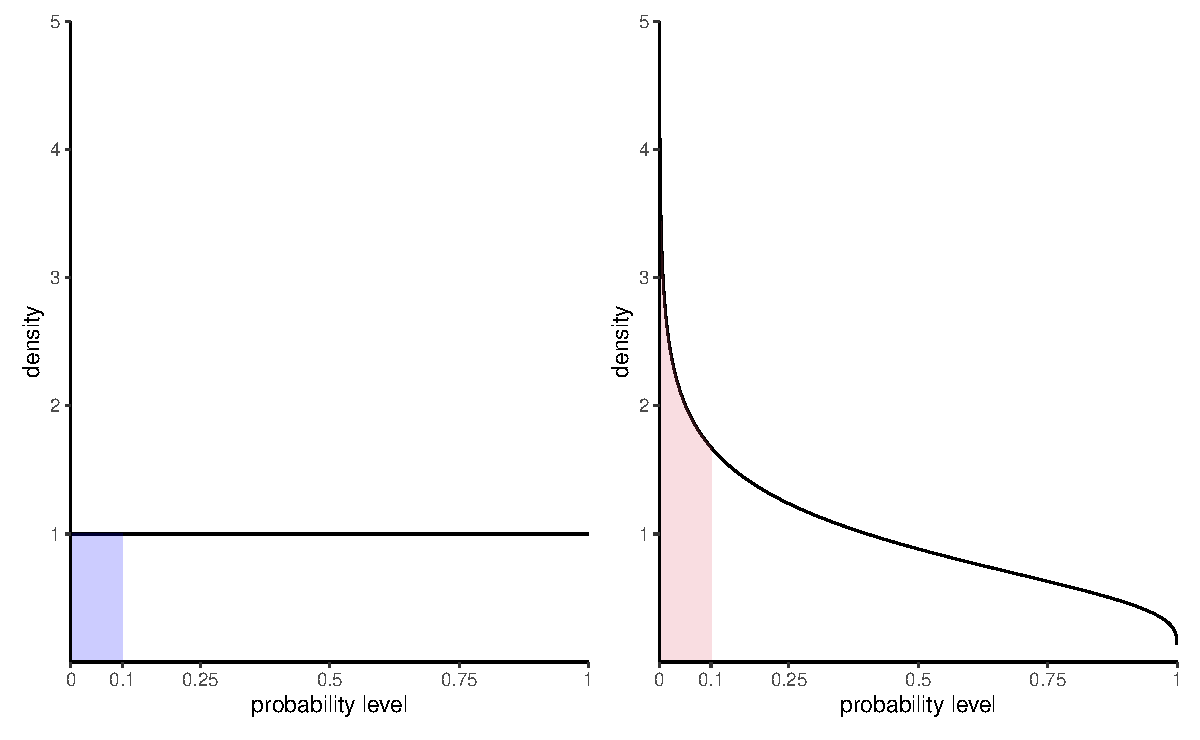
\includegraphics[width=0.85\textwidth,height=\textheight]{inference_files/figure-pdf/fig-power-plots-1.pdf}

}

\caption{\label{fig-power-plots}Densité des valeurs-\(p\) sou
l'hypothèse nulle (gauche) et une alternative avec un ratio signal-bruit
de 0.5 (droite).}

\end{figure}%

Il existe généralement trois façons d'obtenir des lois nulles pour
évaluer le degré de preuve contre l'hypothèse nulle

\begin{itemize}
\tightlist
\item
  les calculs exacts (combinatoires)
\item
  la théorie des grands échantillons (appelée « régime asymptotique »
  dans le jargon statistique)
\item
  les méthodes de simulation Monte Carlo.
\end{itemize}

Bien que souhaitable, la première méthode n'est applicable que dans des
cas simples (comme le calcul de la probabilité d'obtenir deux six en
lançant deux dés identiques). La deuxième méthode est la plus couramment
utilisée en raison de sa généralité et de sa facilité d'utilisation (en
particulier dans les temps anciens où la puissance de calcul était
rare), mais elle ne donne pas de bons résultats avec des échantillons de
petite taille (où la noti de « trop petit » dépend du contexte et du
test). La dernière approche peut être utilisée pour approcher la
distribution nulle dans de nombreux scénarios, mais elle ajoute une
couche d'aléatoire et les coûts de calcul supplémentaires n'en valent
parfois pas la peine.

Prenons l'exemple d'un test d'hypothèse bilatéral pour la moyenne au
population \(\mathscr{H}_0:\mu=0\) contre \(\mathscr{H}_a:\mu \neq 0.\)
Si l'échantillon provient d'une (population de) loi normale
\(\mathsf{normale}(\mu, \sigma^2),\) on peut démontrer que, si
\(\mathscr{H}_0\) est vraie et donc \(\mu=0\)), la statistique de test
\begin{align*}
T = \frac{\overline{X}}{S/\sqrt{n}}
\end{align*} suit une loi de Student-\(t\) avec \(n-1\) degrés de
liberté, dénotée \(\mathsf{Student}_{n-1}.\) À partir de cette loi
nulle, on peut calculer la valeur-\emph{p} (ou bien à partir d'une table
ou d'un logiciel statistique). Puisque la distribution Student-\(t\) est
symétrique autour de \(0,\) on peut calculer la valeur-\emph{p} comme
\(P = 2\times\Pr(T > |t|),\) où \(T \sim \mathsf{Student}_{n-1}.\)

\section{Intervalle de confiance}\label{intervalle-de-confiance}

Un \textbf{intervalle de confiance} est une manière alternative de
rapporter les conclusions d'un test, en ce sens qu'on fournit une
estimation ponctuelle de \(\hat{\theta}\) avec une marge d'erreur.
L'intervalle de confiance donne donc une indication de la variabilité de
la procédure d'estimation. Un intervalle de confiance de Wald à
\((1-\alpha)\) pour un paramètre \(\theta\) est de la forme
\begin{align*}
[\widehat{\theta} + \mathfrak{q}_{\alpha/2}\mathrm{se}(\widehat{\theta}), \widehat{\theta} +\mathfrak{q}_{1-\alpha/2}\times \mathrm{se}(\widehat{\theta})]
\end{align*} où \(\mathfrak{q}_{\alpha}\) dénote le quantile d'ordre
\(\alpha \in (0,1)\) de la loi nulle de la statistique de Wald,
\begin{align*}
T =\frac{\widehat{\theta}-\theta}{\mathrm{se}(\widehat{\theta})},
\end{align*} et où \(\theta\) représente la valeur du paramètre
\(\theta\) (supposé fixe, mais inconnu) de la population.

Par exemple, pour un échantillon aléatoire \(X_1, \ldots, X_n\)
provenant d'une loi \(\mathsf{normale}(\mu, \sigma),\) l'intervalle de
confiance à \((1-\alpha)\) pour la moyenne (dans la population) \(\mu\)
est \begin{align*}
\overline{X} \pm t_{n-1, \alpha/2} \frac{S}{\sqrt{n}}
\end{align*} où \(t_{n-1, \alpha/2}\) est le quantile d'ordre
\(1-\alpha/2\) de la loi Student-\(t\) avec \(n-1\) degrés de libertés.

Les bornes de l'intervalle de confiance sont aléatoires puisque
\(\widehat{\theta}\) et \(\mathrm{se}(\widehat{\theta})\) sont des
variable aléatoires: leurs valeurs observées changent d'un échantillon à
un autre. Avant qu'on calcule l'intervalle de confiance, il y a une
probabilité de \(1-\alpha\) que \(\theta\) soit contenu dans
l'intervalle \textbf{aléatoire} symmétrique
\((\widehat{\theta} - \mathfrak{q}_{\alpha/2} \; \mathrm{se}(\widehat{\theta}), \widehat{\theta} + \mathfrak{q}_{\alpha/2} \; \mathrm{se}(\widehat{\theta})),\)
où \(\widehat{\theta}\) dénote l'estimateur de \(\theta.\) Une fois
qu'on obtient un échantillon et qu'on calcule les bornes de l'intervalle
de confiance, il n'y a plus de notion de probabilité: la vraie valeur du
paramètre \(\theta\) (inconnue) est soit contenue dans l'intervalle de
confiance, soit pas. La seule interprétation de l'intervalle de
confiance qui soit valable alors est la suivante: si on répète
l'expérience plusieurs fois et qu'à chaque fois on calcule un intervalle
de confiance à \(1-\alpha,\) alors une proportion de \((1-\alpha)\) de
ces intervalles devraient contenir la vraie valeur de \(\theta\) (de la
même manière, si vous lancez une pièce de monnaie équilibrée, vous
devriez obtenir grosso modo une fréquence de 50\% de pile et 50\% de
face, mais chaque lancer donnera un ou l'autre de ces choix). Notre «
confiance » est dans la procédure et non pas dans les valeurs numériques
obtenues pour un échantillon donné.

\begin{figure}[ht!]

\centering{

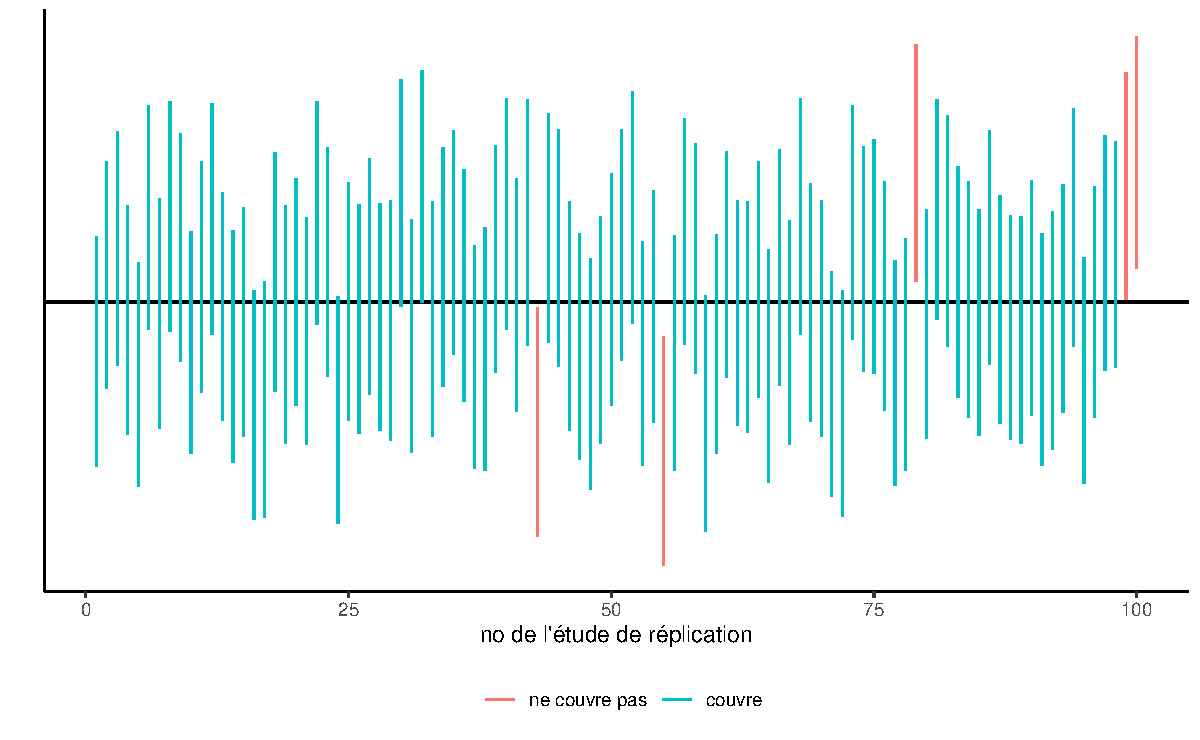
\includegraphics[width=0.85\textwidth,height=\textheight]{inference_files/figure-pdf/fig-intconf-1.pdf}

}

\caption{\label{fig-intconf}Intervalles de confiance à 95\% pour la
moyenne d'une population normale standard pour 100 échantillons
aléatoires. En moyenne, 5\% de ces intervalles (en rouge) n'incluent pas
la vraie valeur de la moyenne de zéro.}

\end{figure}%

Si on s'intéresse seulement à la décision rejeter/ne pas rejeter
\(\mathscr{H}_0,\) l'intervalle de confiance est équivalent à la
valeur-\emph{p} en ce sens qu'il mène à la même décision. L'intervalle
de confiance donne en revanche l'ensemble des valeurs pour lesquelles la
statistique de test ne fournit pas assez de preuves pour rejeter
\(\mathscr{H}_0\): pour un test à niveau \(\alpha,\) on ne rejetterait
aucune des valeurs contenues dans l'intervalle de confiance de niveau
\(1-\alpha.\) Si la valeur-\emph{p} est inférieure à \(\alpha,\) la
valeur postulée pour \(\theta\) est donc hors de l'intervalle de
confiance calculé. À l'inverse, la valeur-\emph{p} ne donne la
probabilité d'obtenir un résultat aussi extrême sous l'hypothèse nulle
que pour une seule valeur numérique, mais permet de quantifier
précisément à quel point le résultat est extrême.

\section{Conclusion}\label{conclusion}

La valeur-\emph{p} nous permet de faire une décision quant aux
hypothèses du test. Si \(\mathscr{H}_0\) est vraie, la valeur-\emph{p}
suit une loi uniforme. \href{https://xkcd.com/1478/}{Si la
valeur-\emph{p} est petite}, ça veut dire que le fait d'observer une
statistique de test égal ou encore plus extrême que \(T=t\) est peu
probable, et donc nous aurons tendance de croire que \(\mathscr{H}_0\)
n'est pas vraie. Il y a pourtant toujours un risque sous-jacent de
commettre un erreur quand on prend une décision. En statistique, il y a
\href{https://xkcd.com/2303/}{deux types d'erreurs}:

\begin{itemize}
\tightlist
\item
  erreur de type I: on rejette \(\mathscr{H}_0\) alors que
  \(\mathscr{H}_0\) est vraie
\item
  erreur de type II: on ne rejette pas \(\mathscr{H}_0\) alors que
  \(\mathscr{H}_0\) est fausse
\end{itemize}

Ces deux erreurs ne sont pas égales: on cherche souvent à contrôler
l'erreur de type I (une erreur judiciaire, condamner un innocent). Pour
se prémunir face à ce risque, on fixe préalablement un niveau de
tolérance. Plus notre seuil de tolérance \(\alpha\) est grand, plus on
rejette souvent l'hypothèse nulle même si cette dernière est vraie. La
valeur de \(\alpha \in (0, 1)\) est la probabilité qu'on rejette
\(\mathscr{H}_0\) quand \(\mathscr{H}_0\) est en fait vraie.
\begin{align*}
\alpha = \Pr{\!}_0\left(\text{ rejeter } \mathscr{H}_0\right).
\end{align*} Comme chercheur, on choisit ce niveau \(\alpha\);
habituellement \(1\)\%, \(5\)\% ou \(10\)\%. La probabilité de commettre
une erreur de type I est \(\alpha\) seulement si le modèle nul postulé
pour \(\mathscr{H}_0\) est correctement spécifié (sic) et correspond au
modèle générateur des données.

Le choix du statu quo (typiquement \(\mathscr{H}_0\)) s'explique plus
facilement avec un exemple médical. Si vous voulez prouver qu'un nouveau
traitement est meilleur que l'actuel (ou l'absence de traitement), vous
devez démontrer hors de tout doute raisonnable que ce dernier ne cause
pas de torts aux patients et offre une nette amélioration (pensez à
Didier Raoult et ses allégations non-étayées voulant que
l'hydrochloroquine, un antipaludique, soit efficace face au virus de la
Covid19).

\begin{longtable}[]{@{}
  >{\raggedright\arraybackslash}p{(\columnwidth - 4\tabcolsep) * \real{0.3333}}
  >{\centering\arraybackslash}p{(\columnwidth - 4\tabcolsep) * \real{0.3333}}
  >{\centering\arraybackslash}p{(\columnwidth - 4\tabcolsep) * \real{0.3333}}@{}}
\toprule\noalign{}
\begin{minipage}[b]{\linewidth}\raggedright
\textbf{Décision} \textbackslash{} \textbf{vrai modèle}
\end{minipage} & \begin{minipage}[b]{\linewidth}\centering
\(\mathscr{H}_0\)
\end{minipage} & \begin{minipage}[b]{\linewidth}\centering
\(\mathscr{H}_a\)
\end{minipage} \\
\midrule\noalign{}
\endhead
\bottomrule\noalign{}
\endlastfoot
ne pas rejeter \(\mathscr{H}_0\) & \(\checkmark\) & erreur de type II \\
rejeter \(\mathscr{H}_0\) & erreur de type I & \(\checkmark\) \\
\end{longtable}

Pour prendre une décision, on doit comparer la valeur-\emph{p} \(P\)
avec le niveau du test \(\alpha\):

\begin{itemize}
\tightlist
\item
  si \(P < \alpha\) on rejette \(\mathscr{H}_0,\)
\item
  si \(P \geq \alpha\) on ne rejette pas \(\mathscr{H}_0.\)
\end{itemize}

Attention à ne pas confondre niveau du test (probabilité fixée au
préalable par l'expérimentateur) et la valeur-\emph{p} (qui dépend de
l'échantillon). Si vous faites un test à un niveau 5\% la probabilité de
faire une erreur de type I est de 5\% par définition, quelque soit la
valeur de la valeur-\emph{p}. La valeur-\emph{p} s'interprète comme la
probabilité d'obtenir une valeur de la statistique de test égale ou même
plus grande que celle qu'on a observée dans l'échantillon, si
\(\mathscr{H}_0\) est vraie.

\begin{tcolorbox}[enhanced jigsaw, colbacktitle=quarto-callout-caution-color!10!white, title=\textcolor{quarto-callout-caution-color}{\faFire}\hspace{0.5em}{Mise en garde}, leftrule=.75mm, opacityback=0, colframe=quarto-callout-caution-color-frame, breakable, toprule=.15mm, coltitle=black, toptitle=1mm, colback=white, bottomrule=.15mm, bottomtitle=1mm, titlerule=0mm, arc=.35mm, rightrule=.15mm, left=2mm, opacitybacktitle=0.6]

L'\href{https://doi.org/10.1080/00031305.2016.1154108}{\emph{American
Statistical Association (ASA)} a publié une liste de principes}
détaillant les principales erreurs d'interprétation des valeurs-\(p,\)
notamment

\begin{quote}
\begin{enumerate}
\def\labelenumi{(\arabic{enumi})}
\setcounter{enumi}{1}
\tightlist
\item
  Les valeurs-\(p\) ne mesurent pas la probabilité que l'hypothèse
  étudiée est vrai
\end{enumerate}
\end{quote}

\begin{quote}
\begin{enumerate}
\def\labelenumi{(\arabic{enumi})}
\setcounter{enumi}{2}
\tightlist
\item
  Les décisions d'affaires et scientiques ne devraient pas seulement
  être basées sur le fait qu'une valeur-\(p\) est inférieure à un seuil
  spécifié.
\end{enumerate}
\end{quote}

\begin{quote}
\begin{enumerate}
\def\labelenumi{(\arabic{enumi})}
\setcounter{enumi}{3}
\tightlist
\item
  Les analyses statistiques et les valeurs-\(p\) associées ne devraient
  pas être rapportées de manière sélective.
\end{enumerate}
\end{quote}

\begin{quote}
\begin{enumerate}
\def\labelenumi{(\arabic{enumi})}
\setcounter{enumi}{4}
\tightlist
\item
  Les valeurs-\(p,\) ou la significativité statistiques, ne mesurent pas
  la taille de l'effet ou l'importance d'un résultat.
\end{enumerate}
\end{quote}

\end{tcolorbox}

\section{Puissance statistique}\label{puissance-statistique}

Le but du test d'hypothèse est de prouver (hors de tout doute
raisonnable) qu'une différence ou un effet est significatif: par
exemple, si une nouvelle configuration d'un site web (hypothèse
alternative) permet d'augmenter les ventes par rapport au statu quo.
Notre capacité à détecter cette amélioration dépend de la puissance du
test: plus cette dernière est élevée, plus grande est notre capacité à
rejeter \(\mathscr{H}_0\) quand ce dernier est faux.

Quand on ne rejette pas \(\mathscr{H}_0\) et que \(\mathscr{H}_a\) est
en fait vraie, on commet une erreur de type II: cette dernière survient
avec probabilité \(1-\gamma.\) La \textbf{puissance statistique} d'un
test est la probabilité que le test rejette \(\mathscr{H}_0\) alors que
\(\mathscr{H}_0\) est fausse, soit \begin{align*}
\gamma = \Pr{\!}_a(\text{rejeter } \mathscr{H}_0)
\end{align*} Selon le choix de l'alternative, il est plus ou moins
facile de rejeter l'hypothèse nulle en faveur de l'alternative.

\begin{figure}[ht!]

\centering{

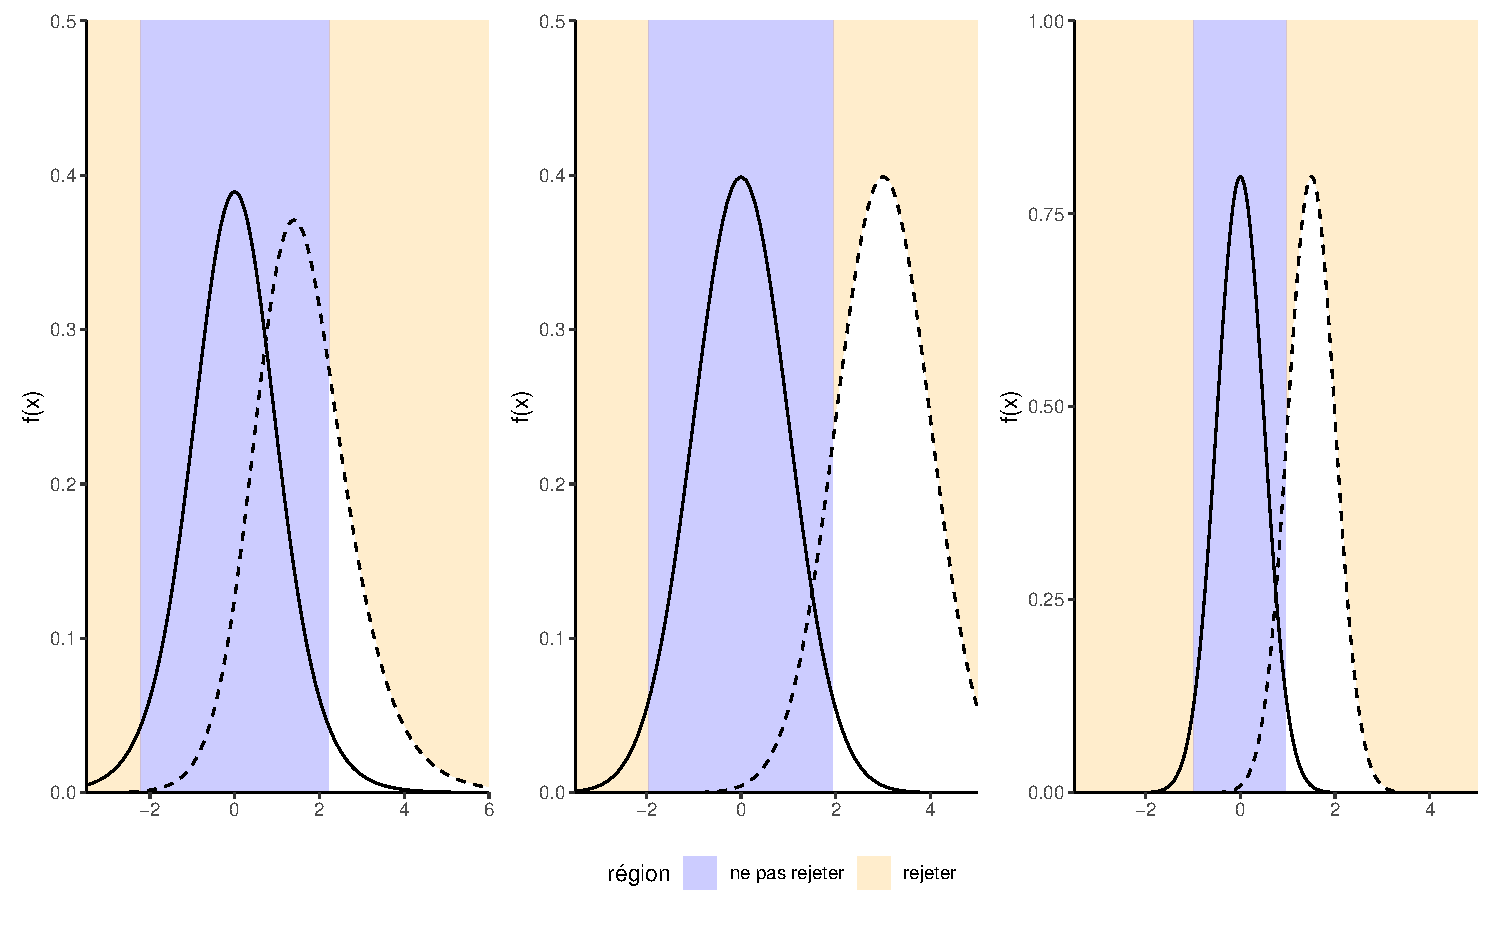
\includegraphics[width=1\textwidth,height=\textheight]{inference_files/figure-pdf/fig-puissance-1.pdf}

}

\caption{\label{fig-puissance}Comparaison de la loi nulle (ligne pleine)
et d'une alternative spécifique pour un test-\(t\) (ligne traitillée).
La puissance correspond à l'aire sous la courbe de la densité de la loi
alternative qui est dans la zone de rejet du test (en blanc). Le panneau
du milieu représente l'augmentation de la puissance suite à
l'augmentation de la taille d'effet (différence moyenne entre groupes
plus élevée) sous l'hypothèse alternative. Le panneau de droite
correspond à un scénario alternatif avec la même taille d'effet, mais
une taille d'échantillon ou une précision plus grande.}

\end{figure}%

On veut qu'un test ait une puissance élevée, c'est-à-dire, le plus près
de 1 possible. Minimalement, la puissance du test devrait être
\(\alpha\) si on rejette l'hypothèse nulle une fraction \(\alpha\) du
temps quand cette dernière est vraie. La puissance dépend de plusieurs
critères, à savoir:

\begin{itemize}
\tightlist
\item
  la taille de l'effet: plus la différence est grande entre la valeur
  postulée \(\theta_0\) du paramètre sous \(\mathscr{H}_0\) et le
  comportement observé, plus il est facile de le détecter (panneau du
  milieu de Figure~\ref{fig-puissance});
\item
  la variabilité: moins les observations sont variables, plus il est
  facile de déterminer que la différence observée est significative (les
  grandes différences sont alors moins plausibles, comme l'illustre le
  panneau de droite de Figure~\ref{fig-puissance});
\item
  la taille de l'échantillon: plus on a d'observations, plus notre
  capacité à détecter une différence significative augmente parce que
  l'erreur-type décroît avec la taille de l'échantillon à un rythme
  (ordinairement) de \(n^{-1/2}.\) La loi nulle devient aussi plus
  concentrée quand la taille de l'échantillon augmente.
\item
  le choix de la statistique de test: par exemple, les statistiques
  basées sur les rangs n'utilisent pas les valeurs numériques qu'à
  travers le rang relatif. Ces tests sont donc moins puissants parce
  qu'ils n'utilisent pas toute l'information dans l'échantillon; en
  contrepartie, ils sont souvent plus robustes en présence de valeurs
  aberrantes et si le modèle est mal spécifié. Les statistiques de test
  que nous choisirons sont souvent standards et parmi les plus
  puissantes qui soient, aussi on ne traitera pas de ce point davantage
  dans le cadre du cours.
\end{itemize}

Pour calculer la puissance d'un test, il faut choisir une alternative
spécifique. Pour des exemples simples de statistiques, on peut obtenir
une formule explicite pour la puissance. Généralement, on détermine la
puissance à l'aide de méthodes de Monte Carlo en simulant des
observations d'une alternative donnée, en calculant la statistique de
test sur le nouvel échantillon simulé et en calculant la valeur-\emph{p}
associée à notre hypothèse nulle de façon répétée. On calcule par la
suite la proportion de tests qui mènent au rejet de l'hypothèse nulle à
niveau \(\alpha,\) ce qui correspond au pourcentage de valeurs-\(p\)
inférieures à \(\alpha.\)

\section{Exemples}\label{exemples}

\begin{example}[Inégalité de genre et tests de
permutation]\protect\hypertarget{exm-rosenjerdee74}{}\label{exm-rosenjerdee74}

Nous examinons les données de Rosen et Jerdee
(\citeproc{ref-Rosen:1974}{1974}), qui étudie les stéréotypes de genre
et leur impact sur la promotion et les opportunités pour les femmes
candidates. L'expérience s'est déroulée en 1972 et les unités
expérimentales, composées de 95 superviseurs bancaires masculins, ont
reçu divers mémorandums et ont été invitées à fournir des évaluations de
candidatures pour un poste de cadre. Ils devaient prendre des décisions
sur la base des informations fournies.

Nous nous intéressons à l'expérience 1 relative à la promotion des
employés: les responsables devaient décider de promouvoir ou non un
employé au poste de directeur de succursale sur la base de
recommandations et d'évaluations du potentiel de relations avec les
clients et les employés. L'intervention des auteurs s'est concentrée sur
la description de la nature (complexité) du travail du gestionnaire
(simple ou complexe) et sur le sexe du candidat (homme ou femme): tous
les dossiers étaient par ailleurs similaires.

Pour des raisons de simplicité, nous ne considérons que le facteur sexe
et nous agrégeons sur le poste pour les \(n=93\) réponses. La table
Tableau~\ref{tbl-rosen-table1} montre le décompte des recommendations
pour chaque possibilité.

\begin{longtable}[t]{lrr}

\caption{\label{tbl-rosen-table1}Recommendations de promotion pour le
poste de gestionnaire de branche selon le sexe de la personne qui
postule.}

\tabularnewline

\toprule
 & male & female\\
\midrule
promouvoir & 32 & 19\\
ne pas promouvoir & 12 & 30\\
\bottomrule

\end{longtable}

L'hypothèse nulle qui nous intéresse ici est que le sexe n'a pas
d'impact, de sorte que la probabilité de promotion est la même pour les
hommes et les femmes. Soit \(p_{\text{h}}\) et \(p_{\text{f}}\) ces
probabilités respectives; nous pouvons donc écrire mathématiquement
l'hypothèse nulle comme \(\mathscr{H}_0: p_{\text{h}} = p_{\text{f}}\)
contre l'alternative \(\mathscr{H}_a: p_{\text{h}} \neq p_{\text{f}}\).

La statistique de test généralement employée pour les tableaux de
contingence est un test du chi carré\footnote{Si vous avez suivi des
  cours de modélisation avancés, il s'agit d'un test de score obtenu en
  ajustant une régression de Poisson avec \texttt{sexe} et
  \texttt{action} comme covariables; l'hypothèse nulle correspondant à
  l'absence de terme d'interaction entre les deux.}, qui compare les
proportions globales de promotion de chaque sous-groupe. La proportion
de l'échantillon pour les hommes est de 32/42 = \textasciitilde76\%,
contre 19/49 =\textasciitilde49\% pour les femmes. Bien que cette
différence de 16 \% semble importante, elle pourrait être trompeuse:
l'erreur type pour les proportions de l'échantillon est d'environ 3.2 \%
pour les hommes et 3.4 \% pour les femmes.

S'il n'y avait pas de discrimination fondée sur le sexe, nous nous
attendrions à ce que la proportion de personnes promues soit la même
dans l'ensemble; elle est de 51/93 ou 0.55 pour l'échantillon regroupé.
Nous pourrions nous contenter de tester la différence moyenne, mais nous
nous appuyons plutôt sur le test de contingence \(X^2_p\) de Pearson
(également appelé test du khi-carré), qui compare les chiffres attendus
(sur la base de taux de promotion égaux) aux chiffres observés,
convenablement normalisés. convenablement normalisés. Si l'écart est
important entre les chiffres attendus et les chiffres observés, cela met
en doute la véracité de l'hypothèse nulle.

Si les effectifs de chaque cellule sont importants, la distribution
nulle du test du chi-deux est bien approximée par une distribution de
\(\chi^2\). La sortie du test comprend la valeur de la statistique,
\(10.79,\) les degrés de liberté de l'approximation \(\chi^2\) et la
valeur \emph{p}, qui donne la probabilité qu'un tirage aléatoire d'une
distribution \(\chi^2_1\) soit plus grand que la statistique de test
observée \textbf{en supposant que l'hypothèse nulle est vraie}. La
valeur \emph{p} est très petite, \(0.001\), ce qui signifie qu'il est
très peu probable qu'un tel résultat soit le fruit du hasard s'il n'y a
pas eu de discrimination fondée sur le sexe.

Une autre solution pour obtenir un point de référence permettant
d'évaluer le caractère exagéré du rapport de cotes observé consiste à
utiliser des simulations: les tests de permutation sont efficaces
{[}illustrés par Jared Wilber{]}
(https://www.jwilber.me/permutationtest/). Considérons une base de
données contenant les données brutes avec 93 lignes, une pour chaque
gestionnaie, avec pour chacune un indicateur d'\texttt{action} et le
\texttt{sexe} de l'employé hypothétique présenté dans la tâche.

\begin{longtable}[t]{ll}

\caption{\label{tbl-dat-long-test-rosen-print}Les cinq premières lignes
de la base de données en format long pour l'expérience 1 de Rosen et
Jerdee (1974).}

\tabularnewline

\toprule
action & sexe\\
\midrule
promouvoir & homme\\
ne pas promouvoir & femme\\
promouvoir & homme\\
ne pas promouvoir & femme\\
ne pas promouvoir & homme\\
\bottomrule

\end{longtable}

Sous l'hypothèse nulle, le sexe n'a aucune incidence sur l'action du
gestionnaire. Cela signifie que nous pourrions dresser un portrait du
monde sans discrimination en mélangeant les étiquettes de sexe de
manière répétée. Ainsi, nous pourrions obtenir une référence en répétant
les étapes suivantes plusieurs fois :

\begin{enumerate}
\def\labelenumi{\arabic{enumi}.}
\tightlist
\item
  permuter les étiquettes pour le \texttt{sexe},
\item
  recréer un tableau de contingence en agrégeant les effectifs,
\item
  calculer une statistique de test pour le tableau simulé.
\end{enumerate}

Comme statistique de test, nous utilisons le rapport des cotes: la
probabilité d'un événement est le rapport entre le nombre de succès et
le nombre d'échecs. Dans notre exemple, il s'agirait du nombre de
dossiers promus par rapport au nombre de dossiers retenus. La
probabilité de promotion d'un homme est de \(32/12,\) alors que celle
d'une femme est de \(19/30.\) Le rapport des cotes pour un homme par
rapport à une femme est donc \(\mathsf{RC}=(32/12) / (19/30)= 4.21.\)
Sous l'hypothèse nulle, \(\mathscr{H}_0: \mathsf{OR}= 1\) (même
probabilité d'être promu) (pourquoi ?)

\begin{figure}[ht!]

\centering{

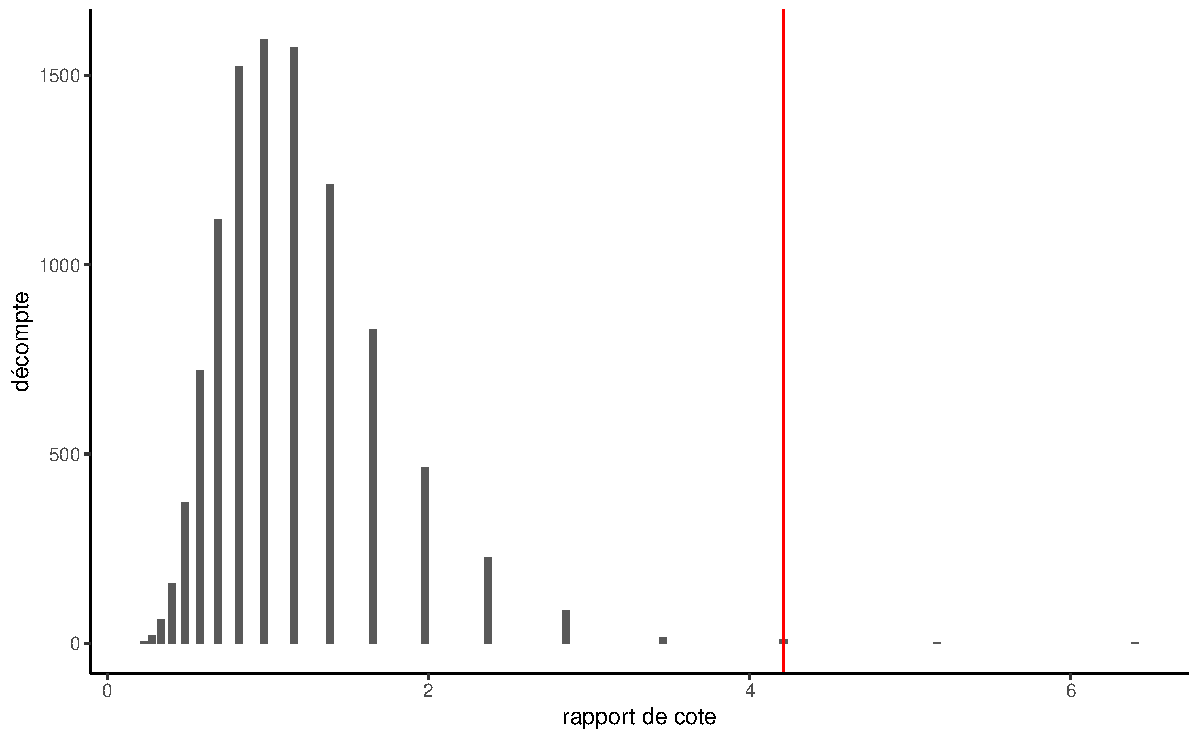
\includegraphics[width=0.85\textwidth,height=\textheight]{inference_files/figure-pdf/fig-infer-odds-ratio-permutation-1.pdf}

}

\caption{\label{fig-infer-odds-ratio-permutation}Histogramme de
simulations de la loi nulle pour le rapport de cote, obtenu par le biais
d'un test de permutation; la ligne verticale rouge indique le rapport de
cote échantillonal.}

\end{figure}%

L'histogramme de la Figure~\ref{fig-infer-odds-ratio-permutation} montre
la distribution du rapport de cotes sur la base de 10 000 permutations.
Il est rassurant de constater que nous obtenons à peu près la même
valeur \emph{p} approximative, ici 0.002.\footnote{La valeur \emph{p}
  obtenue pour le test de permutation changerait d'une exécution à
  l'autre puisque les intrants sont aléatoires. Cependant, la précision
  de la statistique est suffisante pour la prise de décision}.

L'article concluait (à la lumière de ce qui précède et d'autres
expériences)

\begin{quote}
Les résultats ont confirmé l'hypothèse selon laquelle les
administrateurs masculins ont tendance à discriminer les employées dans
les décisions concernant la promotion, le développement et la
supervision du personnel.
\end{quote}

\textbf{Récapitulatif}

\begin{itemize}
\tightlist
\item
  Paramètres du modèle: probabilité de promotion pour les hommes et les
  femmes, respectivement \(p_{\text{h}}\) et \(p_{\text{f}}\).
\item
  Hypothèses: pas de discrimination fondée sur le sexe, ce qui signifie
  une probabilité de promotion égale (hypothèse nulle
  \(\mathscr{H}_0: p_{\text{h}}=p_{\text{f}},\) contre hypothèse
  alternative \(\mathscr{H}_a: p_{\text{h}}\neq p_{\text{f}}\)).
\item
  Statistique de test: (1) test du khi-deux pour les tableaux de
  contingence et (2) rapport de cotes.
\item
  Valeur-\(p\): (1) \(.0010\) et (2) \(.0024\) pour le test de
  permutation.
\item
  Conclusion: rejeter l'hypothèse nulle, car il existe des preuves d'une
  discrimination fondée sur le sexe, avec une probabilité de promotion
  différente pour les hommes et les femmes.
\end{itemize}

Conformément aux directives de l'APA, la statistique \(\chi^2\) serait
présentée sous la forme \(\chi^2(1, n = 93) = 10.79\), \(p = .001\) en
même temps que les effectifs et les proportions de l'échantillon.

\end{example}

\begin{example}[L'élément de surprise d'une prise de contact
inattendue]\protect\hypertarget{exm-LiuRimMinMin2023E1}{}\label{exm-LiuRimMinMin2023E1}

Liu et al. (\citeproc{ref-Liu.Rim.Min.Min:2023}{2023}) étudie les
interactions sociales et l'impact de la surprise sur les personnes qui
contactent de vieilles connaissances de manière inattendue. L'expérience
1 se concentre sur des questionnaires où la condition expérimentale est
l'appréciation perçue du fait d'envoyer une communication à quelqu'un
avec qui on n'a pas correspondu depuis longtemps (par opposition au fait
de se faire contacter). L'étude a utilisé un questionnaire envoyé à 200
adultes américains recrutés sur la plateforme Prolific Academic.
L'indice de réponse consiste en la moyenne de quatre questions mesurées
sur une échelle de Likert allant de 1 à 7, les valeurs les plus élevées
indiquant une plus grande appréciation de la prise de contact.

Nous pouvons commencer par examiner les statistiques sommaires des
variables sociodémographiques (sexe et âge) afin d'évaluer si
l'échantillon est représentatif de la population générale dans son
ensemble. La proportion d'« autres » (comprenant les personnes non
binaires) est beaucoup plus élevée que celle du recensement général, et
la population est plutôt jeune selon
Tableau~\ref{tbl-LRMMS1-summarystat-a}.

\begin{longtable}[t]{lrrrr}

\caption{\label{tbl-LRMMS1-summarystat-a}Statistiques descriptives de
l'âge des participants, et décompte par genre.}

\tabularnewline

\toprule
genre & min & max & moyenne & n\\
\midrule
homme & 18 & 78 & 32.0 & 105\\
femme & 19 & 68 & 36.5 & 92\\
autre & 24 & 30 & 27.7 & 3\\
\bottomrule

\end{longtable}

\begin{longtable}[t]{lrrr}

\caption{\label{tbl-LRMMS1-summarystat-b}Appréciation moyenne
(écart-type), et nombre de participants par condition expérimentale.}

\tabularnewline

\toprule
rôle & moyenne & écart-type & n\\
\midrule
initiateur & 5.50 & 1.28 & 103\\
destinataire & 5.87 & 1.27 & 97\\
\bottomrule

\end{longtable}

Comme il n'y a que deux groupes sans chevauchements (c'est à dire que
les personnes ont un seul rôle), soit initiateur ou destinataire, le
test logique à utiliser est un test-\(t\) pour deux échantillons
indépendants, ou une variante de celui-ci. En utilisant la statistique
du \(t\)-test de Welch, la moyenne et l'écart-type de chaque groupe sont
estimés à l'aide des données fournies.

Le logiciel renvoie comme valeur du test , ce qui conduit au rejet de
l'hypothèse nulle d'absence de différence d'appréciation en fonction du
rôle de l'individu (initiateur ou destinataire). La différence moyenne
estimée est \(\Delta M = -0.37\), 95\% CI \([-0.73, -0.01]\); puisque
\(0\) n'est pas inclus dans l'intervalle de confiance, nous rejetons
également l'hypothèse nulle au niveau 5\%. L'estimation suggère que les
initiateurs sous-estiment l'importance de contacter de manière
inattendue.\footnote{En supposant que la variance de chaque sous-groupe
  soit égale, nous aurions pu utiliser un \(t\)-test à deux échantillons
  à la place. La différence dans la conclusion est insignifiante, avec
  une valeur \emph{p} presque égale}.

\textbf{Récapitulatif}

\begin{itemize}
\tightlist
\item
  Paramètres du modèle: score d'appréciation moyen \(\mu_{\mathrm{i}}\)
  et \(\mu_{\mathrm{d}}\) des initiateurs et des destinataires,
  respectivement.
\item
  Hypothèse: le score d'appréciation attendu est le même pour les
  initiateurs et les destinataires,
  \(\mathscr{H}_0: \mu_{\mathrm{i}}=\mu_{\mathrm{d}}\) contre
  l'alternative
  \(\mathscr{H}_0: \mu_{\mathrm{i}} \neq \mu_{\mathrm{r}}\) qu'ils sont
  différents.
\item
  Statistique de test: test-\(t\) de Welch pour deux échantillons
  indépendants
\item
  Valeur-\(p\): 0.041
\item
  Conclusion: rejet de l'hypothèse nulle, le score moyen d'appréciation
  diffère selon le rôle tenu.
\end{itemize}

\end{example}

\begin{example}[Les communications virtuelles réduisent le nombre
d'idées
créatives]\protect\hypertarget{exm-BrucksLevav22}{}\label{exm-BrucksLevav22}

Une étude de Nature a réalisé une expérience pour voir comment les
communications virtuelles impactent le travail d'équipe en comparant le
nombre d'idées créatives générées par des binômes au cours d'une tempête
d'idée, ainsi que leur qualité telle que mesurée par des arbitres
externes. L'échantillon était composé de 301 paires de participants qui
ont interagi par vidéoconférence ou en face à face.

Les auteurs ont comparé le nombre d'idées créatives, un sous-ensemble
d'idées générées avec un score de créativité supérieur à la moyenne. Le
nombre moyen d'idées créatives pour le face à face est \(7.92\) idées
(écart-type \(3.40\)), comparativement à \(6.73\) idées (écart-type¸
\(3.27\)) pour la vidéoconférence.

Brucks et Levav (\citeproc{ref-Brucks.Levav:2022}{2022}) a utilisé un
modèle de régression binomiale négative: dans leur modèle, le nombre
moyen d'idées créatives générées est \begin{align*}
\mathsf{E}(\texttt{ncreative}) = \exp(\beta_0 + \beta_1 \texttt{video})
\end{align*} où \(\texttt{video}=0\) si la paire se trouve dans la même
pièce et \(\texttt{video}=1\) si elle interagit plutôt par
vidéoconférence.

Le nombre moyen d'idées pour la vidéoconférence est donc
\(\exp(\beta_1)\) multiplié par celui du face à face: l'estimation du
facteur multiplicatif est \(\exp(\beta_1)\) est \(0.85\) 95\% CI
\([0.77, 0.94]\).

L'absence de différence entre les conditions expérimentales se traduit
par l'hypothèse nulle \(\mathscr{H}_0: \beta_1=0\) vs
\(\mathscr{H}_0: \beta_1 \neq 0\) ou, de manière équivalente,
\(\mathscr{H}_0: \exp(\beta_1)=1\). Le test du rapport de vraisemblance
comparant le modèle de régression avec et sans \(\texttt{video}\) la
statistique est \(R=9.89\) (valeur-\(p\) basée sur \(\chi^2_1\) de
\(.002\)). Nous concluons que le nombre moyen d'idées est différent, les
statistiques sommaires suggérant que les paires virtuelles génèrent
moins d'idées.

Si nous avions eu recours à un test-\(t\) pour deux échantillons
indépendants, nous aurions trouvé une différence moyenne dans le nombre
d'idées créatives de \(\Delta M = 1.19\), 95\% CI \([0.43, 1.95]\),
\(t(299) = 3.09\), \(p = .002\).

Les deux tests reposent sur des hypothèses légèrement différentes, mais
aboutissent à des conclusions similaires: il a de forts indices que le
nombre d'idées créatives est plus faible lorsque les personnes
interagissent par vidéoconférence.

\end{example}

\begin{example}[Prix de billets de trains à grande vitesse
espagnols]\protect\hypertarget{exm-prix-trains-tests}{}\label{exm-prix-trains-tests}

La compagnie nationale de chemin de fer
\href{https://www.renfe.com/}{Renfe} gère les trains régionaux et les
trains à haute vitesse dans toute l'Espagne. Les prix des billets vendus
par Renfe sont
\href{https://www.kaggle.com/thegurusteam/spanish-high-speed-rail-system-ticket-pricing}{aggrégés}
par une compagnie. On s'intéresse ici à une seule ligne,
Madrid--Barcelone. Notre question scientifique est la suivante: est-ce
que le prix des billets pour un aller (une direction) est plus chère
pour un retour? Pour ce faire, on considère un échantillon de 10000
billets entre les deux plus grandes villes espagnoles. On s'intéresse au
billets de TGV vendus (AVE) au tarif Promotionnel. Notre statistique de
test sera simplement la différence de moyenne entre les deux
échantillons: la différence entre le prix en euros d'un train
Madrid--Barcelone (\(\mu_1\)) et le prix d'un billet Barcelone--Madrid
(\(\mu_2\)) est \(\mu_1-\mu_2\) et notre hypothèse nulle est qu'il n'y a
aucune différence de prix, soit \(\mathscr{H}_0: \mu_1-\mu_2=0.\)

On utilise de nouveau le test de Welch pour deux échantillons en
filtrant les données pour ne conserver que les billets au tarif Promo:
la moyenne des billets Barcelone-Madrid est 82.11 euros, ceux pour
Madrid-Barcelone 82.56 euros et la valeur de la statistique de Welch est
-1.33. Si on utilise l'approximation normale, on obtient une
valeur-\(p\) de 0.18.

Plutôt que d'utiliser la loi asymptotique (qui est valide pour de grands
échantillons à cause du théorème central limite), on peut considérer une
approximation sous une hypothèse moins restrictive en supposant que les
données sont échangeables. Sous l'hypothèse nulle, il n'y aucune
différence entre les deux destinations et les étiquettes pour la
destination (une variable catégorielle binaire) sont arbitraires. On
pourrait considérer les mêmes données, mais avec une permutation des
variables explicatives: c'est ce qu'on appelle un
\href{https://www.jwilber.me/permutationtest/}{test de permutation}. On
va recréer deux groupes de taille identique à notre échantillon
original, mais en changeant les observations. On recalcule la
statistique de test sur ces nouvelle données (si on a une poignée
d'observations, il est possible de lister toutes les permutations
possibles; typiquement, il suffit de considérer un grand nombre de
telles permutations, disons 9999). Pour chaque nouveau jeu de données,
on calculera la statistique de test et on calculera le rang de notre
statistique par rapport à cette référence. Si la valeur de notre
statistique observée sur l'échantillon original est extrême en
comparaison, c'est autant de preuves contre l'hypothèse nulle.

\begin{figure}[ht!]

\centering{

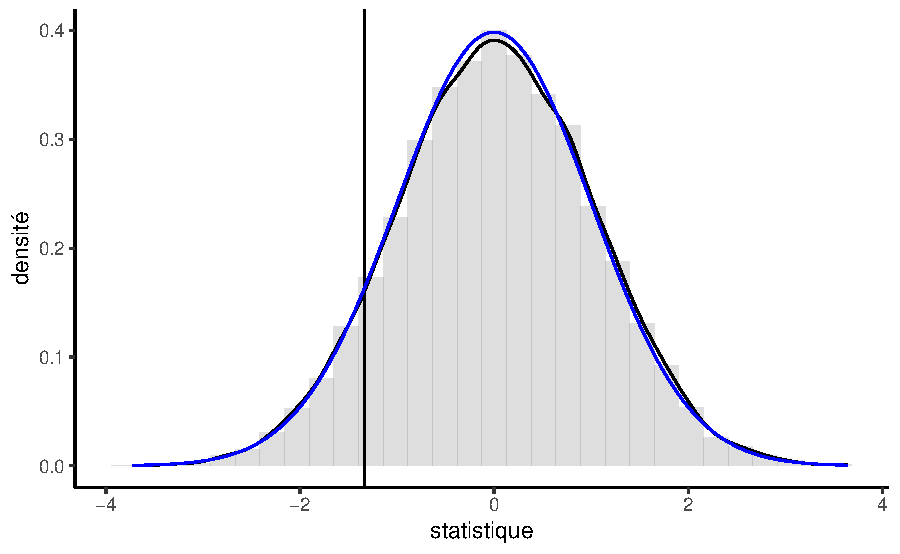
\includegraphics[width=0.85\textwidth,height=\textheight]{inference_files/figure-pdf/fig-renfepermut-1.pdf}

}

\caption{\label{fig-renfepermut}Approximation par permutation de la loi
nulle de la statistique de test de Welch (histogramme et trait noir) et
loi asymptotique normale standard (trait bleu) pour le prix de billets
de trains AVE au tarif promotionnel entre Madrid et Barcelone. La valeur
de la statistique de test de l'échantillon original est représentée par
un trait vertical.}

\end{figure}%

La valeur-\emph{p} du test de permutation, \(0.186,\) est la proportion
de statistiques plus extrêmes que celle observée. Cette valeur-\emph{p}
est quasi-identique à celle de l'approximation de Satterthwaite, à
savoir \(0.182\) (la loi Student-\(t\) est numériquement équivalente à
une loi standard normale avec autant de degrés de liberté), tel que
représenté dans la Figure~\ref{fig-renfepermut}. Malgré que notre
échantillon soit très grand, avec \(n=8059\) observations, la différence
n'est pas jugée significative. Avec un échantillon de deux millions de
billets, on pourrait estimer précisément la moyenne (au centime près):
la différence de prix entre les deux destinations et cette dernière
deviendrait statistiquement significative. Elle n'est pas en revanche
pas pertinente en partique, car une différence de \(0.28\) euros sur un
prix moyen de \(82.56\) euros est quantité négligeable.

\end{example}

\bookmarksetup{startatroot}

\chapter{Inférence basée sur la vraisemblance}\label{vraisemblance}

Ce chapitre traite de modélisation statistique et d'inférence basée sur
la vraisemblance, la méthodologie la plus populaire dans le monde de la
statistique.

\begin{tcolorbox}[enhanced jigsaw, colbacktitle=quarto-callout-important-color!10!white, title=\textcolor{quarto-callout-important-color}{\faExclamation}\hspace{0.5em}{Important}, leftrule=.75mm, opacityback=0, colframe=quarto-callout-important-color-frame, breakable, toprule=.15mm, coltitle=black, toptitle=1mm, colback=white, bottomrule=.15mm, bottomtitle=1mm, titlerule=0mm, arc=.35mm, rightrule=.15mm, left=2mm, opacitybacktitle=0.6]

\textbf{Objectifs d'apprentissage}

\begin{itemize}
\tightlist
\item
  Apprendre la terminologie associée à l'inférence basée sur la
  vraisemblance.
\item
  Dériver des expressions explicites pour l'estimateur du maximum de
  vraisemblance de modèles simples.
\item
  En utilisant l'optimisation numérique, obtenir des estimations de
  paramètres et leurs erreurs-type en utilisant le maximum de
  vraisemblance.
\item
  Utiliser les propriétés de la vraisemblance pour les grands
  échantillons afin d'obtenir des intervalles de confiance et les
  propriétés des tests statistiques.
\item
  Être capable d'utiliser les critères d'information pour la sélection
  des modèles.
\end{itemize}

\end{tcolorbox}

Un modèle statistique spécifie typiquement un mécanisme de génération de
données. Nous postulons ainsi que les données ont été générées à partir
d'une loi de probabilité dotée de \(p\) paramètres
\(\boldsymbol{\theta}.\) L'espace d'échantillonnage est l'ensemble dans
lequel se trouvent les \(n\) observations, tandis que l'espace des
paramètres \(\boldsymbol{\Theta} \subseteq \mathbb{R}^p\) est l'ensemble
des valeurs que peuvent prendre le vecteur de paramètres.

Nous considérons un exemple pour motiver les concepts présentés
ci-après. Supposons qu'on s'intéresse au temps qu'un usager doit
attendre à la station Université de Montréal s'il arrive à 17h59 précise
tous les jours de la semaine, juste à temps pour la prochaine rame de
métro. La base de données \texttt{attente} consistent le temps en
secondes avant que la prochaine rame ne quitte la station. Les données
ont été collectées pendant trois mois et peuvent être traitées comme un
échantillon indépendant. Le panneau gauche de
Figure~\ref{fig-attente-hist} montre un histogramme des observations
\(n=62\) qui vont de \(4\) à \(57\) secondes. Les données sont
positives, notre modèle doit donc tenir compte de cette caractéristique.

\begin{figure}[ht!]

\centering{

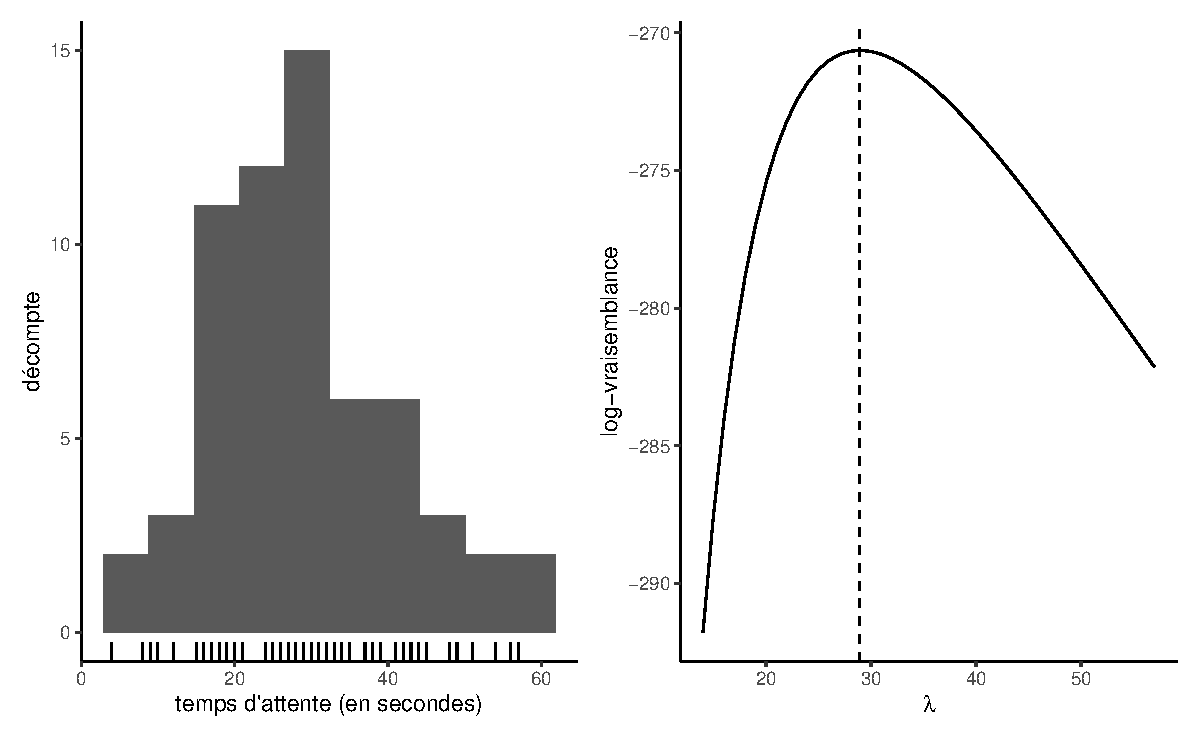
\includegraphics[width=0.85\textwidth,height=\textheight]{vraisemblance_files/figure-pdf/fig-attente-hist-1.pdf}

}

\caption{\label{fig-attente-hist}Histogramme du temps d'attente avec des
traits indiquant les temps observés (gauche) et log-vraisemblance
exponentielle, avec la valeur de l'estimation du maximum de
vraisemblance en traitillé (droite).}

\end{figure}%

\begin{example}[Modèle exponentiel pour les temps
d'attente]\protect\hypertarget{exm-modele-exponentiel}{}\label{exm-modele-exponentiel}

Pour modéliser les temps d'attente, on considère une loi exponentielle
avec paramètre d'échelle \(\lambda\) (Définition~\ref{def-loiexpo}), où
\(\lambda\) est l'espérance (moyenne théorique). Sous un postulat
d'indépendence\footnote{Si \(A\) et \(B\) sont des variables aléatoires
  indépendantes, leur probabilité conjointe est le produit des
  probabilités des événements individuels,
  \(\Pr(A \cup B) = \Pr(A)\Pr(B).\) La même factorisation tient pour la
  fonction de densité ou de masse, lesquelles sont les dérivées de la
  fonction de répartition.}, la densité conjointe des observations
\(y_1, \ldots, y_n\) est \begin{align*}
f(\boldsymbol{y}) = \prod_{i=1}^n f(y_i) =\prod_{i=1}^n  \lambda^{-1} \exp(- y_i/\lambda) = \lambda^{-n} \exp\left(- \sum_{i=1}^n y_i/\lambda\right)
\end{align*} L'espace d'échantillonnage est
\(\mathbb{R}_{+}^n = [0, \infty)^n,\) et l'espace des paramètres est
\((0, \infty).\)

\end{example}

Pour estimer le paramètre d'échelle \(\lambda\) et obtenir des mesures
d'incertitude appropriées, nous avons besoin d'un \textbf{cadre de
modélisation}.

\section{Estimation par maximum de
vraisemblance}\label{estimation-par-maximum-de-vraisemblance}

Pour chaque valeur du paramètre \(\boldsymbol{\theta},\) on obtient une
fonction de densité ou de masse pour les obserations qui varie en
fonction de la compatibilité entre le modèle et les données recueillies.
Cela nous permet d'obtenir une fonction objective pour l'estimation des
paramètres

\begin{definition}[Vraisemblance]\protect\hypertarget{def-vraisemblance}{}\label{def-vraisemblance}

La \textbf{vraisemblance} \(L(\boldsymbol{\theta})\) est une fonction
des paramètres \(\boldsymbol{\theta}\) qui donne la probabilité (ou
densité) d'observer un échantillon selon une loi postulée, en traitant
les observations comme fixes, \begin{align*}
L(\boldsymbol{\theta}; \boldsymbol{y}) = f(\boldsymbol{y}; \boldsymbol{\theta}),
\end{align*} où \(f(\boldsymbol{y}; \boldsymbol{\theta})\) désigne la
densité ou la fonction de masse conjointe du \(n\)-vecteur des
observations.

Si ces dernières sont indépendantes, la densité conjointe se factorise
en un produit de densité unidimensionnelle pour chaque observation et la
vraisemblance devient alors \begin{align*}
L(\boldsymbol{\theta}; \boldsymbol{y})=\prod_{i=1}^n f_i(y_i; \boldsymbol{\theta}) = f_1(y_1; \boldsymbol{\theta}) \times \cdots \times f_n(y_n; \boldsymbol{\theta}).
\end{align*} La fonction de log-vraisemblance correspondante pour des
données indépendantes et identiquement distribuées est \begin{align*}
\ell(\boldsymbol{\theta}; \boldsymbol{y}) = \sum_{i=1}^n \ln f(y_i; \boldsymbol{\theta})
\end{align*}

\end{definition}

\begin{example}[Données
dépendantes]\protect\hypertarget{exm-markov}{}\label{exm-markov}

La fonction de densité conjointe ne se factorise que pour les données
indépendantes, mais une décomposition séquentielle alternative peut
s'avérer utile. Par exemple, nous pouvons écrire la densité conjointe
\(f(y_1, \ldots, y_n)\) en utilisant la factorisation \begin{align*}
f(\boldsymbol{y}) = f(y_1) \times f(y_2 \mid y_1) \times \ldots f(y_n \mid y_1, \ldots, y_n)
\end{align*} en termes de densitées conditionnelles. Une telle
décomposition est particulièrement utile pour les séries temporelles, où
les données sont ordonnées du temps \(1\) au temps \(n\) et où les
modèles relient généralement l'observation \(y_n\) à son passé. Par
exemple, le processus \(\mathsf{AR}(1)\) stipule que
\(Y_t \mid Y_{t-1}=y_{t-1} \sim \mathsf{normale}(\alpha + \beta y_{t-1}, \sigma^2)\)
et nous pouvons simplifier la log-vraisemblance en utilisant la
propriété de Markov, qui stipule que la réalisation actuelle dépend du
passé, \(Y_t \mid Y_1, \ldots, Y_{t-1},\) uniquement à travers la valeur
la plus récente \(Y_{t-1}\). La log-vraisemblance devient donc
\begin{align*}
\ell(\boldsymbol{\theta}) = \ln f(y_1) + \sum_{i=2}^n f(y_i \mid y_{i-1}).
\end{align*}

\end{example}

\begin{definition}[Estimateur du maximum de
vraisemblance]\protect\hypertarget{def-emv}{}\label{def-emv}

L'\textbf{estimateur du maximum de vraisemblance} (EMV)
\(\widehat{\boldsymbol{\theta}}\) est la valeur du vecteur qui maximise
la vraisemblance, \begin{align*}
\widehat{\boldsymbol{\theta}} = \mathrm{arg max}_{\boldsymbol{\theta} \in \boldsymbol{\Theta}} L(\boldsymbol{\theta}; \boldsymbol{y}).
\end{align*} Le logarithme naturel \(\ln\) est une transformation
monotone, il est donc préférable de calculer les EMV sur l'échelle
logarithmique pour éviter les imprécisions numériques et maximiser de
manière équivalente la log-vraisemblance
\(\ell(\boldsymbol{\theta}; \boldsymbol{y}) = \ln L(\boldsymbol{\theta}; \boldsymbol{y}).\)\footnote{Puisque
  dans la plupart des cas on a un produit de densités, prendre le
  logarithme transforme un produit de termes potentiellement petits en
  une somme de log densités, ce qui est plus facile côté dérivation et
  plus stable du point de vue du calcul numérique.}

\end{definition}

Si nous supposons que notre modèle est correct, nous nous attendons à
observer ce qui a été réalisé, et nous trouvons donc le vecteur de
paramètres qui rend l'échantillon le plus susceptible d'avoir été généré
par notre modèle. Plusieurs propriétés de l'estimateur du maximum de
vraisemblance le rendent intéressant pour l'inférence. L'estimateur du
maximum de vraisemblance est efficace, c'est-à-dire qu'il présente
l'erreur quadratique moyenne asymptotique la plus faible de tous les
estimateurs. L'estimateur du maximum de vraisemblance est également
\textbf{convergent}, c'est-à-dire qu'il approche de la vraie valeur du
paramètre inconnu à mesure que la taille de l'échantillon augmente
(asymptotiquement sans biais).

La plupart du temps, nous allons recourir à des routines d'optimisation
numérique pour trouver la valeur de l'estimation du maximum de
vraisemblance, ou parfois dériver des expressions explicites pour
l'estimateur, à partir de la log-vraisemblance. Le panneau de droite de
Figure~\ref{fig-attente-hist} montre la log-vraisemblance exponentielle,
qui atteint un maximum à \(\widehat{\lambda}=28.935\) secondes, la
moyenne de l'échantillon des observations. La fonction diminue de part
et d'autre de ces valeurs à mesure que les données deviennent moins
compatibles avec le modèle. Compte tenu de l'échelle pour la
log-vraisemblance, ici pour un petit échantillon, il est facile de voir
que l'optimisation directe de la fonction de vraisemblance (plutôt que
de son logarithme naturel) pourrait conduire à un débordement numérique,
puisque \(\exp(-270) \approx 5.5 \times 10^{-118},\) et que les valeurs
logarithmiques inférieures à \(-746\) seraient arrondies à zéro.

\begin{example}[Calcul de l'estimateur du maximum de vraisemblance d'une
loi
exponentielle]\protect\hypertarget{exm-exponential-mle}{}\label{exm-exponential-mle}

La Figure~\ref{fig-attente-hist} révèle que la log-vraisemblance
exponentielle est unimodale. Nous pouvons utiliser le calcul
différentiel pour obtenir une expression explicite pour
\(\widehat{\lambda}\) sur la base de la log-vraisemblance \begin{align*}
\ell(\lambda) = -n \ln\lambda -\frac{1}{\lambda} \sum_{i=1}^n y_i.
\end{align*} Si on calcule la dérivée première et que l'on fixe cette
dernière à zéro, on obtient \begin{align*}
\frac{\mathrm{d} \ell(\lambda)}{\mathrm{d} \lambda}  = -\frac{n}{\lambda} + \frac{1}{\lambda^2} \sum_{i=1}^n y_i = 0.
\end{align*} En réarrangeant cette expression pour amener \(-n/\lambda\)
à droite de l'égalité, et en multipliant les deux côtés par
\(\lambda^2>0,\) on obtient que le point d'inflexion se situe à
\(\widehat{\lambda} = \sum_{i=1}^n y_i / n.\) La dérivée deuxième de la
log vraisemblance est
\(\mathrm{d}^2 \ell(\lambda)/\mathrm{d} \lambda^2 = n(\lambda^{-2} - 2\lambda^{-3}\overline{y}),\)
et si on évalue cette dernière à \(\lambda = \overline{y}\), on trouve
une valeur négative, \(-n/\overline{y}^2.\) Cela confirme que
\(\widehat{\lambda}\) est la valeur où la fonction atteint son maximum.

\end{example}

\begin{example}[Échantillons de loi
normale]\protect\hypertarget{exm-emv-normal}{}\label{exm-emv-normal}

Supposons que nous disposions de \(n\) observations de loi normale de
paramètres de moyenne \(\mu\) et de variance \(\sigma^2\), où
\(Y_i \sim \mathsf{normale}(\mu, \sigma^2)\) sont indépendants.
Rappelons que la densité de la loi normale est \begin{align*}
f(y; \mu, \sigma^2)=\frac{1}{(2\pi \sigma^2)^{1/2}}\exp\left\{-\frac{1}{2\sigma^2}(x-\mu)^2\right\}.
\end{align*} Pour une réalisation \(y_1, \ldots, y_n\) tirée d'un
échantillon aléatoire simple, la vraisemblance est \begin{align*}
L(\mu, \sigma^2; \boldsymbol{y})=&\prod_{i=1}^n\frac{1}{({2\pi \sigma^2})^{1/2}}\exp\left\{-\frac{1}{2\sigma^2}(y_i-\mu)^2\right\}\\
=&(2\pi \sigma^2)^{-n/2}\exp\left\{-\frac{1}{2\sigma^2}\sum_{i=1}^n(y_i-\mu)^2\right\}.
\end{align*} et la log-vraisemblance s'écrit \begin{align*}
\ell(\mu, \sigma^2; \boldsymbol{y})=-\frac{n}{2}\ln(2\pi) -\frac{n}{2}\ln(\sigma^2)-\frac{1}{2\sigma^2}\sum_{i=1}^n (y_i-\mu)^2.
\end{align*} On peut montrer que les estimateurs du maximum de
vraisemblance pour les deux paramètres sont \begin{align*}
\widehat{\mu}=\overline{Y}=\frac{1}{n} \sum_{i=1}^n Y_i, \qquad \widehat{\sigma}^2=\frac{1}{n}\sum_{i=1}^n (Y_i-\overline{Y})^2.
\end{align*}

Le fait que l'estimateur de la moyenne théorique \(\mu\) soit la moyenne
de l'échantillon est assez intuitif et on peut montrer que l'estimateur
est sans biais pour \(\mu\). L'estimateur sans biais de la variance de
l'échantillon est \begin{align*}
S^2=\frac{1}{n-1} \sum_{i=1}^n (Y_i-\overline{Y})^2.
\end{align*} Puisque \(\widehat{\sigma}^2=(n-1)/n S^2\), il s'ensuit que
l'estimateur du maximum de vraisemblance de \(\sigma^2\) est biaisé,
mais les deux estimateurs sont convergents et s'approcheront donc de la
vraie valeur \(\sigma^2\) pour \(n\) suffisamment grand.

\end{example}

\begin{example}[Moindres carrés
ordinaires]\protect\hypertarget{exm-mco-mle}{}\label{exm-mco-mle}

Le cas des données normalement distribuées est intimement lié à la
régression linéaire et aux moindres carrés ordinaires: en supposant la
normalité des erreurs, les estimateurs des moindres carrés de
\(\boldsymbol{\beta}\) coïncident avec l'estimateur du maximum de
vraisemblance de \(\boldsymbol{\beta}\).

Le modèle de régression linéaire spécifie que
\(Y_i \sim \mathsf{normale}(\mathbf{X}_i\boldsymbol{\beta}, \sigma^2)\),
ou de manière équivalente \begin{align*}
Y_i=\beta_0+\beta_1 \mathrm{X}_{i1}+\beta_2 \mathrm{X}_{i2}+\ldots +\beta_p \mathrm{X}_{ip} + \varepsilon_i, \qquad  (i=1, \ldots, n),
\end{align*} avec des aléas
\(\varepsilon_i \sim \mathsf{normale}(0, \sigma^2)\). Le modèle linéaire
a \(p+2\) paramètres (\(\boldsymbol{\beta}\) et \(\sigma^2\)) et la
log-vraisemblance est \begin{align*}
\ell(\boldsymbol{\theta})&=-\frac{n}{2} \ln(2\pi)-\frac{n}{2} \ln (\sigma^2) -\frac{1}{2\sigma^2}\left\{(\boldsymbol{y}-\mathbf{X}\boldsymbol{\beta})^\top(\boldsymbol{y}-\mathbf{X}\boldsymbol{\beta})\right\}^2.
\end{align*} Maximiser la log-vraisemblance par rapport à
\(\boldsymbol{\beta}\) équivaut à minimiser la somme des erreurs
quadratiques \(\|\boldsymbol{y} - \widehat{\boldsymbol{y}}\|^2\). Cette
fonction objective étant la même que celle des moindres carrés, il
s'ensuit que l'estimateur des moindres carrés
\(\widehat{\boldsymbol{\beta}}\) pour les paramètres de la moyenne est
aussi l'estimateur du maximum de vraisemblance si les aléas ont la même
variance \(\sigma^2\), quelle que soit la valeur de cette dernière.
L'estimateur du maximum de vraisemblance \(\widehat{\sigma}^2\) est donc
\begin{align*}
\widehat{\sigma}^2=\max_{\sigma^2} \ell(\widehat{\boldsymbol{\beta}}, \sigma^2).
\end{align*} La log-vraisemblance, en omettant tout terme ou constante
qui n'est pas fonction de \(\sigma^2\), est \begin{align*}
\ell(\widehat{\boldsymbol{\beta}}, \sigma^2)
&\propto-\frac{1}{2}\left\{n\ln\sigma^2+\frac{1}{\sigma^2}(\boldsymbol{y}-\mathbf{X}\hat{\boldsymbol{\beta}})^\top(\boldsymbol{y}-\mathbf{X}\hat{\boldsymbol{\beta}})\right\}.
\end{align*} En différenciant chaque terme par rapport à \(\sigma^2\) et
en fixant le gradient à zéro, on obtient l'estimateur du maximum de
vraisemblance \begin{align*}
\widehat{\sigma}^2=\frac{1}{n}(\boldsymbol{Y}-\mathbf{X}\hat{\boldsymbol{\beta}})^\top(\boldsymbol{Y}-\mathbf{X}\hat{\boldsymbol{\beta}})= \frac{1}{n} \sum_{i=1}^n e_i^2= \frac{\mathsf{SS}_e}{n};
\end{align*} où \(\mathsf{SS}_e\) est la somme des carrés des résidus.
L'estimateur sans biais habituel de \(\sigma^2\) calculé par le logiciel
est \(S^2=\mathsf{SS}_e/(n-p-1)\), où le dénominateur est la taille de
l'échantillon \(n\) moins le nombre de paramètres de la moyenne
\(\boldsymbol{\beta}\), soit \(p+1\).

\end{example}

\begin{proposition}[Invariance des estimateurs du maximum de
vraisemblance]\protect\hypertarget{prp-invariance-emv}{}\label{prp-invariance-emv}

Si \(g(\boldsymbol{\theta}): \mathbb{R}^p \mapsto \mathbb{R}^k\) pour
\(k \leq p\) est une fonction des paramètres, alors
\(g(\widehat{\boldsymbol{\theta}})\) est l'estimateur du maximum de
vraisemblance de cette fonction.

\end{proposition}

La propriété d'invariance explique l'utilisation répandue de
l'estimation du maximum de vraisemblance. Par exemple, après avoir
estimé le paramètre \(\lambda,\) nous pouvons maintenant utiliser le
modèle pour dériver d'autres quantités d'intérêt et obtenir les
``meilleures'' estimations gratuitement. Par exemple, nous pourrions
calculer l'estimation du maximum de vraisemblance de la probabilité
d'attendre plus d'une minute,
\(\Pr(T>60) = \exp(-60/\widehat{\lambda})= 0.126.\) On peut utiliser la
fonction de répartition \texttt{pexp} dans \textbf{R},

\begin{Shaded}
\begin{Highlighting}[]
\CommentTok{\# Note: la paramétrisation usuelle dans R pour la loi exponentielle}
\CommentTok{\# est en terme d\textquotesingle{}intensité (réciproque du paramètre d\textquotesingle{}échelle)}
\FunctionTok{pexp}\NormalTok{(}\AttributeTok{q =} \DecValTok{60}\NormalTok{, }\AttributeTok{rate =} \DecValTok{1}\SpecialCharTok{/}\FunctionTok{mean}\NormalTok{(attente), }\AttributeTok{lower.tail =} \ConstantTok{FALSE}\NormalTok{)}
\CommentTok{\#\textgreater{} [1] 0.126}
\end{Highlighting}
\end{Shaded}

Un autre intérêt de la propriété d'invariance est la possibilité de
calculer l'EMV dans la paramétrisation la plus simple, ce qui est
pratique si le support est contraint. Si \(g\) est une fonction
bijective de \(\boldsymbol{\theta},\) par exemple si \(\theta >0,\)
maximiser le modèle paramétré en terme de \(g(\theta) = \ln \theta\) ou
de \(g(\theta) = \ln(\theta) - \ln(1-\theta) \in \mathbb{R}\) si
\(0 \leq \theta \leq 1,\) élimine les contraintes pour l'optimisation
numérique.

\begin{definition}[Score et
information]\protect\hypertarget{def-information}{}\label{def-information}

Soit \(\ell(\boldsymbol{\theta}),\)
\(\boldsymbol{\theta} \in \boldsymbol{\Theta} \subseteq \mathbb{R}^p,\)
la fonction de log-vraisemblance. Le gradient (ou vecteur de dérivée
première) de la log-vraisemblance
\(U(\boldsymbol{\theta}) = \partial \ell(\boldsymbol{\theta}) / \partial \boldsymbol{\theta}\)
est appelé fonction de \textbf{score}.

L'\textbf{information observée} est la hessienne (matrice de dérivée
deuxième) du négatif de la log-vraisemblance \begin{align*}
j(\boldsymbol{\theta}; \boldsymbol{y})=-\frac{\partial^2 \ell(\boldsymbol{\theta}; \boldsymbol{y})}{\partial \boldsymbol{\theta} \partial \boldsymbol{\theta}^\top}.
\end{align*} En pratique, on évalue cette fonction à l'estimation du
maximum de vraisemblance \(\widehat{\boldsymbol{\theta}},\) d'où le
terme information observée pour désigner plutôt
\(j(\widehat{\boldsymbol{\theta}}).\) Sous des conditions de régularité,
l'\textbf{information de Fisher} est \begin{align*}
i(\boldsymbol{\theta}) = \mathsf{E}\left\{U(\boldsymbol{\theta}; \boldsymbol{Y}) U(\boldsymbol{\theta}; \boldsymbol{Y})^\top\right\} = \mathsf{E}\left\{j(\boldsymbol{\theta}; \boldsymbol{Y})\right\}
\end{align*} La différence est qu'on prend l'espérance de chaque
fonction des observations à l'intérieur des entrées de la matrice. Quand
elle évaluée au point \(\widehat{\boldsymbol{\theta}}\), l'information
de Fisher mesure la variance du score, ou la courbure de ce dernier. La
matrice de Fisher et la matrice d'information sont toutes deux
symmétriques.

\end{definition}

\begin{example}[Information pour le modèle
exponentiel]\protect\hypertarget{exm-exponentiel-info}{}\label{exm-exponentiel-info}

L'information de Fisher et observée pour un échantillon aléatoire simple
du modèle exponentiel, \(Y_1, \ldots, Y_n,\), paramétré en terme
d'échelle \(\lambda,\) est \begin{align*}
j(\lambda; \boldsymbol{y}) &= -\frac{\partial^2 \ell(\lambda)}{\partial \lambda^2} = \frac{n}{\lambda^{2}} + \frac{2}{n\lambda^{3}}\sum_{i=1}^n y_i \\
i(\lambda) &= \frac{n}{\lambda^{2}} + \frac{2}{n\lambda^{3}}\sum_{i=1}^n \mathsf{E}(Y_i)  = \frac{n}{\lambda^{2}}
\end{align*} puisque \(\mathsf{E}(Y_i) = \lambda\) et que l'espérance
est un opérateur linéaire. On trouve que
\(i(\widehat{\lambda}) = j(\widehat{\lambda}) = n/\overline{y}^2\), mais
cette égalité ne tient qu'à l'EMV.

\end{example}

Le modèle exponentiel peut s'avérer restrictif pour adéquatement
capturer nos données, c'est pourquoi nous considérons une loi de Weibull
comme généralisation.

\begin{definition}[Loi de
Weibull]\protect\hypertarget{def-weibull}{}\label{def-weibull}

La fonction de répartition d'une variable aléatoire de loi
\textbf{Weibull}, de paramètres d'échelle \(\lambda>0\) et de forme
\(\alpha>0\) est \begin{align*}
F(x; \lambda, \alpha) &= 1 - \exp\left\{-(x/\lambda)^\alpha\right\}, \qquad x \geq 0, \lambda>0, \alpha>0,
\end{align*} alors que sa densité est \begin{align*}
f(x; \lambda, \alpha) &= \frac{\alpha}{\lambda^\alpha} x^{\alpha-1}\exp\left\{-(x/\lambda)^\alpha\right\}, \qquad x \geq 0, \lambda>0, \alpha>0.
\end{align*} La fonction quantile, qui est l'inverse de la fonction de
répartition, est \(Q(p) = \lambda\{-\ln(1-p)\}^{1/\alpha}.\) La loi
Weibull inclut la loi exponentielle comme cas spécial quand
\(\alpha=1.\) L'espérance de
\(Y \sim \mathsf{Weibull}(\lambda, \alpha)\) est
\(\mathsf{E}(Y) = \lambda \Gamma(1+1/\alpha).\)

\end{definition}

\begin{example}[Score et information d'une loi
Weibull]\protect\hypertarget{exm-weibull-emv}{}\label{exm-weibull-emv}

La log-vraisemblance d'un échantillon aléatoire simple de taille \(n\)
dont la réalisation est dénotée \(y_1, \ldots, y_n\), tirée d'une loi
\(\mathsf{Weibull}(\lambda, \alpha)\), est \begin{align*}
\ell(\lambda, \alpha) = n \ln(\alpha) - n\alpha\ln(\lambda) + (\alpha-1) \sum_{i=1}^n \ln y_i  - \lambda^{-\alpha}\sum_{i=1}^n y_i^\alpha.
\end{align*} Le gradient de cette fonction est\footnote{Par exemple, en
  utilisant une calculatrice symbolique.} \begin{align*}
U(\lambda, \alpha) = \begin{pmatrix}\frac{\partial \ell(\lambda, \alpha)}{\partial \lambda} \\
\frac{\partial \ell(\lambda, \alpha)}{\partial \alpha} \end{pmatrix} &= 
\begin{pmatrix}
 -\frac{n\alpha}{\lambda} +\alpha\lambda^{-\alpha-1}\sum_{i=1}^n y_i^\alpha
 \\
 \frac{n}{\alpha} - n \ln(\lambda) + \sum_{i=1}^n \ln y_i  - \sum_{i=1}^n \left(\frac{y_i}{\lambda}\right)^{\alpha} \times\ln\left(\frac{y_i}{\lambda}\right).
 \end{pmatrix}
\end{align*} et l'information observée est \begin{align*}
j(\lambda, \alpha) &= - \begin{pmatrix}
\frac{\partial^2 \ell(\lambda, \alpha)}{\partial \lambda^2} &  \frac{\partial^2 \ell(\lambda, \alpha)}{\partial \lambda \partial \alpha} \\ \frac{\partial^2 \ell(\lambda, \alpha)}{\partial \alpha \partial \lambda} & \frac{\partial^2 \ell(\lambda, \alpha)}{\partial \alpha^2}
\end{pmatrix} 
\\&= \begin{pmatrix}
\lambda^{-2}\left\{-n\alpha + \alpha(\alpha+1)\sum_{i=1}^n (y_i/\lambda)^2\right\} & \lambda^{-1}\sum_{i=1}^n [1-(y_i/\lambda)^\alpha\{1+\alpha\ln(y_i/\lambda)\}]\\ \lambda^{-1}\sum_{i=1}^n [1-(y_i/\lambda)^\alpha\{1+\alpha\ln(y_i/\lambda)\}]& n\alpha^{-2} + \sum_{i=1}^n (y_i/\lambda)^\alpha \{\ln(y_i/\theta)\}^2
\end{pmatrix}
\end{align*}

\end{example}

\begin{proposition}[Optimisation basée sur le
gradient]\protect\hypertarget{prp-gradient}{}\label{prp-gradient}

Pour obtenir l'estimateur du maximum de vraisemblance, nous trouverons
généralement la valeur du vecteur \(\boldsymbol{\theta}\) qui résout le
vecteur de score, c'est-à-dire
\(U(\widehat{\boldsymbol{\theta}})=\boldsymbol{0}_p.\) Cela revient à
résoudre simultanément un système de \(p\) équations en fixant à zéro la
dérivée première par rapport à chaque élément de
\(\boldsymbol{\theta}\). Si \(j(\widehat{\boldsymbol{\theta}})\) est une
matrice définie positive (c'est-à-dire que toutes ses valeurs propres
sont positives), alors le vecteur \(\widehat{\boldsymbol{\theta}}\)
maximise la fonction de log-vraisemblance et est l'estimateur du maximum
de vraisemblance.

Nous pouvons utiliser une variante de l'algorithme de Newton--Raphson si
la vraisemblance est trois fois différentiable et si l'estimateur du
maximum de vraisemblance ne se trouve pas sur la frontière de l'espace
des paramètres. Si nous considérons une valeur initiale
\(\boldsymbol{\theta}^{\dagger},\) alors une expansion en série de
Taylor du premier ordre de la vraisemblance du score dans un voisinage
\(\boldsymbol{\theta}^{\dagger}\) de l'EMV
\(\widehat{\boldsymbol{\theta}}\) donne \begin{align*}
\boldsymbol{0}_p & = U(\widehat{\boldsymbol{\theta}}) \stackrel{\cdot}{\simeq} \left.
\frac{\partial \ell(\boldsymbol{\theta})}{\partial \boldsymbol{\theta}} \right|_{\boldsymbol{\theta} = \boldsymbol{\theta}^{\dagger}} + \left.
\frac{\partial^2 \ell(\boldsymbol{\theta})}{\partial \boldsymbol{\theta} \partial \boldsymbol{\theta}^\top}\right|_{\boldsymbol{\theta} = \boldsymbol{\theta}^{\dagger}}(\widehat{\boldsymbol{\theta}} - \boldsymbol{\theta}^{\dagger})\\&=U(\boldsymbol{\theta}^{\dagger}) - j(\boldsymbol{\theta}^{\dagger})(\widehat{\boldsymbol{\theta}} - \boldsymbol{\theta}^{\dagger}).
\end{align*} En réarrangeant cette expression pour isoler
\(\widehat{\boldsymbol{\theta}}\) (pourvu que la matrice \(p \times p\)
d'information observée \(j(\widehat{\boldsymbol{\theta}})\) soit
inversible à l'EMV), on obtient \begin{align*}
\widehat{\boldsymbol{\theta}} \stackrel{\cdot}{\simeq} \boldsymbol{\theta}^{\dagger} + 
j^{-1}(\boldsymbol{\theta}^{\dagger})U(\boldsymbol{\theta}^{\dagger}).
\end{align*} Cela suggère l'utilisation d'une procédure itérative: à
partir d'une valeur de départ \(\boldsymbol{\theta}^{\dagger}\) dans le
voisinage du mode, on applique le schéma de mise à jour jusqu'à ce que
le gradient soit approximativement nul. Si la valeur est éloignée du
mode, l'algorithme peut diverger. Pour éviter cela, nous pouvons
multiplier le terme
\(j^{-1}(\boldsymbol{\theta}^{\dagger})U(\boldsymbol{\theta}^{\dagger})\)
par un facteur d'amortissement \(c<1\). Une variante de l'algorithme,
appelée score de Fisher, utilise l'information de Fisher
\(i(\boldsymbol{\theta})\) au lieu de l'information observée,
\(j(\boldsymbol{\theta}),\) pour des raisons de stabilité numérique et
pour éviter les situations où cette dernière n'est pas définie positive.
Il s'agit de la routine d'optimisation utilisée dans la fonction
\texttt{glm} de \textbf{R}.

\end{proposition}

\begin{example}[Estimateurs du maximum de vraisemblance d'un échantillon
Weibull]\protect\hypertarget{exm-evm-weibull}{}\label{exm-evm-weibull}

Nous nous tournons vers l'optimisation numérique pour obtenir
l'estimation du maximum de vraisemblance de la loi de Weibull, en
l'absence formule explicite pour les EMV. À cette fin, il faut écrire
une fonction qui encodent la log-vraisemblance, ici la somme des
contributions de la log-densité. La fonction \texttt{nll\_weibull}
ci-dessous prend comme premier argument le vecteur de paramètres,
\texttt{pars}, et renvoie la valeur négative de la log-vraisemblance que
nous souhaitons minimiser\footnote{La plupart des algorithmes
  d'optimisation minimisent les fonctions par rapport à leurs arguments,
  nous minimisons donc la log-vraisemblance négative, ce qui équivaut à
  maximiser la log-vraisemblance}. Nous codons également le gradient,
bien que nous puissions recourir à la différenciation numérique. Nous
utilisons ensuite \texttt{optim}, la routine d'optimisation par défaut
de \textbf{R}, pour minimiser \texttt{nll\_weibull}. La fonction renvoie
une liste contenant un code de convergence (\texttt{0} indiquant la
convergence), les EMV dans \texttt{par}, la log-vraisemblance
\(\ell(\widehat{\boldsymbol{\theta}})\) et la hessienne, qui est la
matrice d'information observée évaluée à
\(\widehat{\boldsymbol{\theta}}.\) La surface de log-vraisemblance, pour
les paires de vecteurs d'échelle et de forme
\(\boldsymbol{\theta} = (\lambda, \alpha),\) est représentée dans la
Figure~\ref{fig-weibull-profile}. Nous pouvons voir que l'algorithme a
convergé vers le maximum de vraisemblance et vérifier que le score
satisfait \(U(\widehat{\boldsymbol{\theta}}) = 0\) à la valeur optimale
retournée.

\begin{Shaded}
\begin{Highlighting}[]
\CommentTok{\# Charger les données}
\FunctionTok{data}\NormalTok{(attente, }\AttributeTok{package =} \StringTok{"hecstatmod"}\NormalTok{)}

\CommentTok{\# Négatif de la log vraisemblance pour un échantillon Weibull}
\NormalTok{nll\_weibull }\OtherTok{\textless{}{-}} \ControlFlowTok{function}\NormalTok{(pars, y) \{}
  \CommentTok{\# Gérer le cas de paramètres négatifs (impossible)}
  \ControlFlowTok{if}\NormalTok{ (}\FunctionTok{isTRUE}\NormalTok{(}\FunctionTok{any}\NormalTok{(pars }\SpecialCharTok{\textless{}=} \DecValTok{0}\NormalTok{))) \{}
    \FunctionTok{return}\NormalTok{(}\FloatTok{1e10}\NormalTok{) }\CommentTok{\# retourner une valeur large finie (pour éviter les messages d\textquotesingle{}avertissement)}
\NormalTok{  \}}
  \SpecialCharTok{{-}} \FunctionTok{sum}\NormalTok{(}\FunctionTok{dweibull}\NormalTok{(}
    \AttributeTok{x =}\NormalTok{ y,}
    \AttributeTok{scale =}\NormalTok{ pars[}\DecValTok{1}\NormalTok{],}
    \AttributeTok{shape =}\NormalTok{ pars[}\DecValTok{2}\NormalTok{],}
    \AttributeTok{log =} \ConstantTok{TRUE}
\NormalTok{  ))}
\NormalTok{\}}
\CommentTok{\# Gradient du négatif de la fonction de log vraisemblance Weibull}
\NormalTok{gr\_nll\_weibull }\OtherTok{\textless{}{-}} \ControlFlowTok{function}\NormalTok{(pars, y) \{}
\NormalTok{  scale }\OtherTok{\textless{}{-}}\NormalTok{ pars[}\DecValTok{1}\NormalTok{]}
\NormalTok{  shape }\OtherTok{\textless{}{-}}\NormalTok{ pars[}\DecValTok{2}\NormalTok{]}
\NormalTok{  n }\OtherTok{\textless{}{-}} \FunctionTok{length}\NormalTok{(y)}
\NormalTok{  grad\_ll }\OtherTok{\textless{}{-}} \FunctionTok{c}\NormalTok{(}
    \AttributeTok{scale =} \SpecialCharTok{{-}}\NormalTok{n }\SpecialCharTok{*}\NormalTok{ shape }\SpecialCharTok{/}\NormalTok{ scale }\SpecialCharTok{+}\NormalTok{ shape }\SpecialCharTok{*}\NormalTok{ scale}\SpecialCharTok{\^{}}\NormalTok{(}\SpecialCharTok{{-}}\NormalTok{shape }\SpecialCharTok{{-}} \DecValTok{1}\NormalTok{) }\SpecialCharTok{*} \FunctionTok{sum}\NormalTok{(y}\SpecialCharTok{\^{}}\NormalTok{shape),}
    \AttributeTok{shape =}\NormalTok{ n }\SpecialCharTok{/}\NormalTok{ shape }\SpecialCharTok{{-}}\NormalTok{ n }\SpecialCharTok{*} \FunctionTok{log}\NormalTok{(scale) }\SpecialCharTok{+} \FunctionTok{sum}\NormalTok{(}\FunctionTok{log}\NormalTok{(y)) }\SpecialCharTok{{-}}
      \FunctionTok{sum}\NormalTok{(}\FunctionTok{log}\NormalTok{(y }\SpecialCharTok{/}\NormalTok{ scale) }\SpecialCharTok{*}\NormalTok{ (y }\SpecialCharTok{/}\NormalTok{ scale)}\SpecialCharTok{\^{}}\NormalTok{shape)}
\NormalTok{  )}
  \FunctionTok{return}\NormalTok{(}\SpecialCharTok{{-}}\NormalTok{grad\_ll)}
\NormalTok{\}}

\CommentTok{\# Utiliser les EMV du modèle exponentiel pour l\textquotesingle{}initialisation}
\NormalTok{valinit }\OtherTok{\textless{}{-}} \FunctionTok{c}\NormalTok{(}\FunctionTok{mean}\NormalTok{(attente), }\DecValTok{1}\NormalTok{)}
\CommentTok{\# Vérifier préalablement que le gradient est correct!}
\CommentTok{\# La commande retourne TRUE si la dérivée numérique égale sa version analytique à tolérance donnée}
\FunctionTok{isTRUE}\NormalTok{(}\FunctionTok{all.equal}\NormalTok{(}
\NormalTok{  numDeriv}\SpecialCharTok{::}\FunctionTok{grad}\NormalTok{(nll\_weibull, }\AttributeTok{x =}\NormalTok{ valinit, }\AttributeTok{y =}\NormalTok{ attente),}
  \FunctionTok{gr\_nll\_weibull}\NormalTok{(}\AttributeTok{pars =}\NormalTok{ valinit, }\AttributeTok{y =}\NormalTok{ attente),}
  \AttributeTok{check.attributes =} \ConstantTok{FALSE}
\NormalTok{))}
\CommentTok{\#\textgreater{} [1] TRUE}
\CommentTok{\# Optimisation numérique avec optim}
\NormalTok{opt\_weibull }\OtherTok{\textless{}{-}} \FunctionTok{optim}\NormalTok{(}
  \AttributeTok{par =}\NormalTok{ valinit,}
  \CommentTok{\# valeurs initiales}
  \AttributeTok{fn =}\NormalTok{ nll\_weibull,}
  \CommentTok{\# passer la fonction à optimiser, son premier argument doit être le vecteur de paramètres}
  \AttributeTok{gr =}\NormalTok{ gr\_nll\_weibull,}
  \CommentTok{\# gradient (optionnel)}
  \AttributeTok{method =} \StringTok{"BFGS"}\NormalTok{,}
  \CommentTok{\# algorithme BFGS est basé sur le gradient, une alternative robuste est"Nelder"}
  \AttributeTok{y =}\NormalTok{ attente,}
  \CommentTok{\# vecteur d\textquotesingle{}observations passées en argument additionnel à "fn"}
  \AttributeTok{hessian =} \ConstantTok{TRUE} \CommentTok{\# retourner la matrice de dérivée secondes évaluée aux EMV}
\NormalTok{) }
\CommentTok{\# Alternative avec un Newton}
\CommentTok{\# nlm(f = nll\_weibull, p = valinit, hessian = TRUE, y = attente)}
\CommentTok{\# Estimations du maximum de vraisemblance}
\NormalTok{(mle\_weibull }\OtherTok{\textless{}{-}}\NormalTok{ opt\_weibull}\SpecialCharTok{$}\NormalTok{par)}
\CommentTok{\#\textgreater{} [1] 32.6  2.6}
\CommentTok{\# Vérifier la convergence numérique à l\textquotesingle{}aide du gradient}
\FunctionTok{gr\_nll\_weibull}\NormalTok{(mle\_weibull, }\AttributeTok{y =}\NormalTok{ attente)}
\CommentTok{\#\textgreater{}     scale     shape }
\CommentTok{\#\textgreater{} 0.0000142 0.0001136}
\CommentTok{\# Vérifier que la hessienne est positive définite}
\CommentTok{\# Toutes les valeurs propres sont positives}
\CommentTok{\# Si oui, on a trouvé un maximum et la matrice est invertible}
\FunctionTok{isTRUE}\NormalTok{(}\FunctionTok{all}\NormalTok{(}\FunctionTok{eigen}\NormalTok{(opt\_weibull}\SpecialCharTok{$}\NormalTok{hessian)}\SpecialCharTok{$}\NormalTok{values }\SpecialCharTok{\textgreater{}} \DecValTok{0}\NormalTok{))}
\CommentTok{\#\textgreater{} [1] TRUE}
\end{Highlighting}
\end{Shaded}

\end{example}

\section{Loi d'échantillonnage}\label{loi-duxe9chantillonnage}

La \textbf{loi d'échantillonnage} d'un estimateur
\(\widehat{\boldsymbol{\theta}}\) est la loi de probabilité induite par
les données aléatoires sous-jacentes.

Supposons que nous disposons d'un échantillon aléatoire simple, de sorte
que la log-vraisemblance est constitutée d'une somme de \(n\) termes et
que l'information s'accumule linéairement avec la taille de
l'échantillon. Nous dénotons la vraie valeur du vecteur de paramètres
inconnu \(\boldsymbol{\theta}_0.\) Sous des conditions de régularité
appropriées, cf.~section 4.4.2 de Davison
(\citeproc{ref-Davison:2003}{2003}), pour un échantillon de grande
taille \(n,\) nous pouvons effectuer une série de Taylor du score et
appliquer le théorème de la limite centrale à la moyenne résultante
puisque \(U(\boldsymbol{\theta})\) et \(i(\boldsymbol{\theta})\) sont la
somme de \(n\) variables aléatoires indépendantes, et que
\(\mathsf{E}\{U(\boldsymbol{\theta})\}=\boldsymbol{0}_p,\) et
\(\mathsf{Var}\{U(\boldsymbol{\theta})\}=i(\boldsymbol{\theta}),\)
l'application du théorème de la limite centrale et de la loi des grands
nombres donne \begin{align*}
i(\boldsymbol{\theta}_0)^{-1/2}U(\boldsymbol{\theta}_0) \stackrel{\cdot}{\sim}\mathsf{normale}_p(\boldsymbol{0}, \mathbf{I}_p).
\end{align*}

On peut utiliser ce résultat pour obtenir une approximation à la loi
d'échantillonnage des estimateurs du maximum de vraisemblance de
\(\widehat{\boldsymbol{\theta}},\) \begin{align*}
\widehat{\boldsymbol{\theta}} \stackrel{\cdot}{\sim} \mathsf{normale}_p\{\boldsymbol{\theta}_0, i^{-1}(\boldsymbol{\theta})\}
\end{align*} ou la matrice de covariance est l'inverse de l'information
de Fisher. En pratique, puisque la valeur des paramètres
\(\boldsymbol{\theta}_0\) est inconnue, on remplace la covariance soit
par \(i^{-1}(\widehat{\boldsymbol{\theta}})\) ou par l'inverse de
l'information observée, \(j^{-1}(\widehat{\boldsymbol{\theta}}).\) Cela
est justifié par le fait que les deux matrices d'informations
\(i(\widehat{\boldsymbol{\theta}})\) et
\(j(\widehat{\boldsymbol{\theta}})\) convergent vers
\(i(\boldsymbol{\theta})\) quand \(n \to \infty\).

Au fur et à mesure que la taille de l'échantillon augmente, l'estimateur
du maximum de vraisemblance \(\widehat{\boldsymbol{\theta}}\) devient
centré autour de la valeur \(\boldsymbol{\theta}_0\) qui minimise
l'écart entre le modèle et le véritable processus de génération des
données. Dans les grands échantillons, la loi d'échantillonnage de
l'estimateur du maximum de vraisemblance est approximativement
quadratique.

\begin{example}[Matrice de covariance et erreurs-type pour le modèle de
Weibull]\protect\hypertarget{exm-Weibull-se}{}\label{exm-Weibull-se}

Nous utilisons la sortie de notre procédure d'optimisation pour obtenir
la matrice d'information observée et les erreurs-type pour les
paramètres du modèle de Weibull. Ces dernières sont simplement la racine
carrée des entrées diagonales de l'information observée évaluée aux EMV,
\([\mathrm{diag}\{j^{-1}(\widehat{\boldsymbol{\theta}})\}]^{1/2}\).

\begin{Shaded}
\begin{Highlighting}[]
\CommentTok{\# La hessienne du négatif de la log vraisemblance, évaluée aux EMV}
\CommentTok{\# est la matrice d\textquotesingle{}information observée}
\NormalTok{obsinfo\_weibull }\OtherTok{\textless{}{-}}\NormalTok{ opt\_weibull}\SpecialCharTok{$}\NormalTok{hessian}
\NormalTok{vmat\_weibull }\OtherTok{\textless{}{-}} \FunctionTok{solve}\NormalTok{(obsinfo\_weibull)}
\CommentTok{\# Erreurs{-}type}
\NormalTok{se\_weibull }\OtherTok{\textless{}{-}} \FunctionTok{sqrt}\NormalTok{(}\FunctionTok{diag}\NormalTok{(vmat\_weibull))}
\end{Highlighting}
\end{Shaded}

\end{example}

Une fois que l'on a les estimations du maximum de vraisemblance et les
erreurs-type, on peut dériver des intervalles de confiance ponctuels de
Wald pour les paramètres de \(\boldsymbol{\theta}.\) Si la quantité
d'intérêt est une transformation des paramètres du modèle, on peut
utiliser le résultat suivant pour procéder.

\begin{proposition}[Normalité asymptotique et
transformations]\protect\hypertarget{prp-transformation}{}\label{prp-transformation}

Le résultat de normalité asymptotique peut être utilisé pour dériver les
erreurs standard pour d'autres quantités d'intérêt. Si
\(\phi = g(\boldsymbol{\theta})\) est une fonction différentiable de
\(\boldsymbol{\theta}\) dont le gradient est non-nul lorsque évalué à
\(\widehat{\boldsymbol{\theta}}\), alors
\(\widehat{\phi} \stackrel{\cdot}{\sim}\mathsf{normale}(\phi_0, \mathrm{V}_\phi),\)
with
\(\mathrm{V}_\phi = \nabla \phi^\top \mathbf{V}_{\boldsymbol{\theta}} \nabla \phi,\)
où
\(\nabla \phi=[\partial \phi/\partial \theta_1, \ldots, \partial \phi/\partial \theta_p]^\top.\)
La matrice de covariance et le gradient sont évalués aux estimations du
maximum de vraisemblance \(\widehat{\boldsymbol{\theta}}.\) Ce résultat
se généralise aux fonctions vectorielles
\(\boldsymbol{\phi} \in \mathbb{R}^k\) pour \(k \leq p,\) où
\(\nabla \phi\) est la jacobienne de la transformation.

\end{proposition}

\begin{example}[Probabilité d'attente pour un modèle
exponentiel.]\protect\hypertarget{exm-transformation-exp}{}\label{exm-transformation-exp}

Considérons les données sur le temps d'attente dans le métro et la
probabilité d'attendre plus d'une minute,
\(\phi=g(\lambda) = \exp(-60/\lambda).\) L'estimation du maximum de
vraisemblance est, par invariance, \(0.126\) et le gradient de \(g\) par
rapport au paramètre d'échelle est
\(\nabla \phi = \partial \phi / \partial \lambda = 60\exp(-60/\lambda)/\lambda^2.\)

\begin{Shaded}
\begin{Highlighting}[]
\CommentTok{\# Exemple de dérivation des erreurs{-}type pour une}
\CommentTok{\# transformation des paramètres}
\CommentTok{\# Ici, on calcule Pr(Y\textgreater{}60) selon le modèle exponentiel}
\NormalTok{lambda\_hat }\OtherTok{\textless{}{-}} \FunctionTok{mean}\NormalTok{(attente)}
\CommentTok{\# Définir la fonction d\textquotesingle{}intérêt}
\NormalTok{phi\_hat }\OtherTok{\textless{}{-}} \FunctionTok{exp}\NormalTok{(}\SpecialCharTok{{-}}\DecValTok{60} \SpecialCharTok{/}\NormalTok{ lambda\_hat)}
\CommentTok{\# jacobien de la transformation}
\NormalTok{dphi }\OtherTok{\textless{}{-}} \ControlFlowTok{function}\NormalTok{(lambda) \{}
  \DecValTok{60} \SpecialCharTok{*} \FunctionTok{exp}\NormalTok{(}\SpecialCharTok{{-}}\DecValTok{60} \SpecialCharTok{/}\NormalTok{ lambda) }\SpecialCharTok{/}\NormalTok{ (lambda}\SpecialCharTok{\^{}}\DecValTok{2}\NormalTok{)}
\NormalTok{\}}
\CommentTok{\# variance du paramètre exponentiel}
\NormalTok{V\_lambda }\OtherTok{\textless{}{-}}\NormalTok{ lambda\_hat}\SpecialCharTok{\^{}}\DecValTok{2} \SpecialCharTok{/} \FunctionTok{length}\NormalTok{(attente)}
\CommentTok{\# variance de Pr(Y\textgreater{}60) via la méthode delta}
\NormalTok{V\_phi }\OtherTok{\textless{}{-}} \FunctionTok{dphi}\NormalTok{(lambda\_hat)}\SpecialCharTok{\^{}}\DecValTok{2} \SpecialCharTok{*}\NormalTok{ V\_lambda}
\CommentTok{\# extraire et imprimer les erreurs{-}type}
\NormalTok{(se\_phi }\OtherTok{\textless{}{-}} \FunctionTok{sqrt}\NormalTok{(V\_phi))}
\CommentTok{\#\textgreater{} [1] 0.0331}
\end{Highlighting}
\end{Shaded}

\end{example}

\section{Tests dérivés de la vraisemblance}\label{sec-testsvrais}

Nous considérons une hypothèse nulle \(\mathscr{H}_0\) qui impose des
restrictions sur les valeurs possibles de \(\boldsymbol{\theta}\), par
rapport à une alternative sans contrainte \(\mathscr{H}_1.\) Nous avons
besoin de deux modèles \textbf{emboîtés} : un modèle \emph{complet} et
un modèle \emph{réduit}, pour lequel l'espace des paramèteres est un
sous-ensemble du modèle complet suite à l'imposition des \(q\)
restrictions. Par exemple, la loi exponentielle est un cas particulier
de la loi de Weibull si \(\alpha=1\).

L'hypothèse nulle \(\mathscr{H}_0\) testée est ``le modèle réduit est
une \textbf{simplification adéquate} du modèle complet''. Soit
\(\widehat{\boldsymbol{\theta}}_0\) les EMV contraints pour le modèle
sous l'hypothèse nulle, et \(\widehat{\boldsymbol{\theta}}\) les EMV du
modèle complet. La vraisemblance fournit trois classes principales de
statistiques pour tester cette hypothèse, soit

\begin{itemize}
\tightlist
\item
  les statistiques des tests du rapport de vraisemblance, notées \(R,\)
  qui mesurent la différence de log vraisemblance (distance verticale)
  entre \(\ell(\widehat{\boldsymbol{\theta}})\) et
  \(\ell(\widehat{\boldsymbol{\theta}}_0).\)
\item
  les statistiques des tests de Wald, notées \(W,\) qui considèrent la
  distance horizontale normalisée entre
  \(\widehat{\boldsymbol{\theta}}\) et
  \(\widehat{\boldsymbol{\theta}}_0.\)
\item
  les statistiques des tests de score de Rao, notées \(S,\) qui
  examinent le gradient repondéré de \(\ell,\) évaluée \emph{uniquement}
  à \(\widehat{\boldsymbol{\theta}}_0\).
\end{itemize}

\begin{figure}[ht!]

\centering{

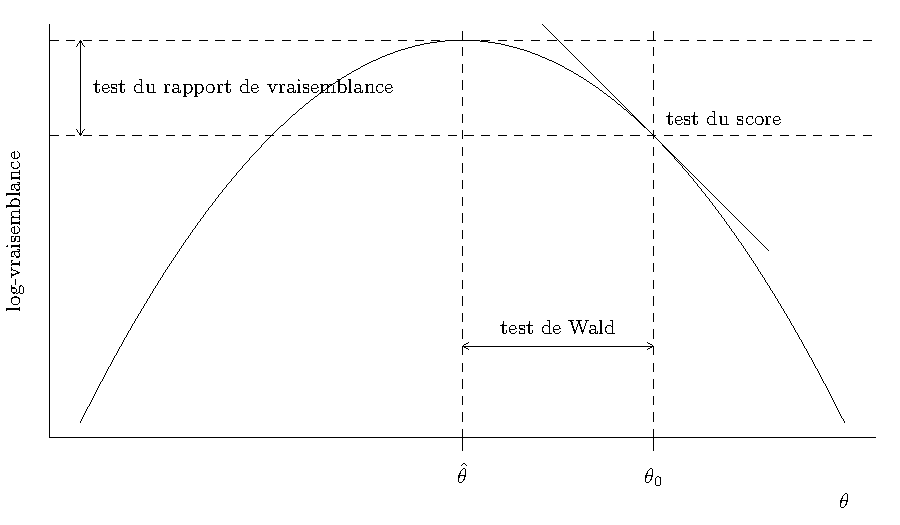
\includegraphics[width=0.85\textwidth,height=\textheight]{images/likelihood_tests_fr.pdf}

}

\caption{\label{fig-courbe-logvraise}Fonction de log vraisemblance et
illustrations des éléments des statistique du score, de Wald et du
rapport de vraisemblance.}

\end{figure}%

Les trois principales classes de statistiques permettant de tester une
hypothèse nulle simple
\(\mathscr{H}_0 : \boldsymbol{\theta}=\boldsymbol{\theta}_0\) par
rapport à l'hypothèse alternative
\(\mathscr{H}_a : \boldsymbol{\theta} \neq \boldsymbol{\theta}_0\) sont
\begin{align*}
 W(\boldsymbol{\theta}_0) &= (\widehat{\boldsymbol{\theta}}-\boldsymbol{\theta}_0)^\top j(\widehat{\boldsymbol{\theta}})(\widehat{\boldsymbol{\theta}}-\boldsymbol{\theta}_0), &&(\text{Wald}) \\
 R(\boldsymbol{\theta}_0) &= 2 \left\{ \ell(\widehat{\boldsymbol{\theta}})-\ell(\boldsymbol{\theta}_0)\right\}, &&(\text{rapport de vraisemblance})\\
 S(\boldsymbol{\theta}_0) &= U^\top(\boldsymbol{\theta}_0)i^{-1}(\boldsymbol{\theta}_0)U(\boldsymbol{\theta}_0), && (\text{score})
\end{align*} où \(\boldsymbol{\theta}_0\) est la valeur nulle postulée
du paramètre avec \(q\) restrictions. Si \(q \neq p\), alors on remplace
\(\boldsymbol{\theta}_0\) par l'estimation contrainte
\(\widehat{\boldsymbol{\theta}}_0\).

Asymptotiquement, toutes les statistiques de test sont équivalentes
(dans le sens où elles conduisent aux mêmes conclusions sur
\(\mathscr{H}_0\)), mais elles ne sont pas identiques. Sous
\(\mathscr{H}_0\), les trois statistiques de test suivent une loi
asymptotique \(\chi^2_q\), où les degrés de liberté \(q\) indiquent le
nombre de restrictions.

Si \(\theta\) est un scalaire (cas \(q=1\)), des versions
directionnelles de ces statistiques existent, \begin{align*}
w(\theta_0)&=(\widehat{\theta}-\theta_0)/\mathsf{se}(\widehat{\theta}) &&(\text{Wald}) \\
r({\theta_0}) &= \mathrm{sign}(\widehat{\theta}-\theta)\left[2
\left\{\ell(\widehat{\theta})-\ell(\theta)\right\}\right]^{1/2} &&(\text{racine directionnelle de vraisemblance}) \\
s(\theta_0)&=i^{-1/2}(\theta_0)U(\theta_0) &&(\text{score}) 
\end{align*}

Sous cette forme, si l'hypothèse nulle
\(\mathscr{H}_0: \theta = \theta_0\) est vraie, alors
\(w(\theta_0)\stackrel{\cdot}{\sim} \mathsf{normale}(0,1)\), etc.

La statistique du test du rapport de vraisemblance est normalement la
plus puissante des trois tests (et donc préférable selon ce critère); la
statistique est aussi invariante aux reparamétrages. La statistique de
score \(S\), moins utilisée, nécessite le calcul du score et de
l'information de Fisher, mais n'est évaluée que sous \(\mathscr{H}_0\)
(car par définition \(U(\widehat{\theta})=0\)), elle peut donc être
utile dans les problèmes où les calculs de l'estimateur du maximum de
vraisemblance sous l'alternative sont coûteux ou impossibles. Le test de
Wald est le plus facile à dériver, mais son taux de couverture empirique
peut laisser à désirer si la loi d'échantillonnage de
\(\widehat{\boldsymbol{\theta}}\) est fortement asymétrique.

\begin{figure}[ht!]

\centering{

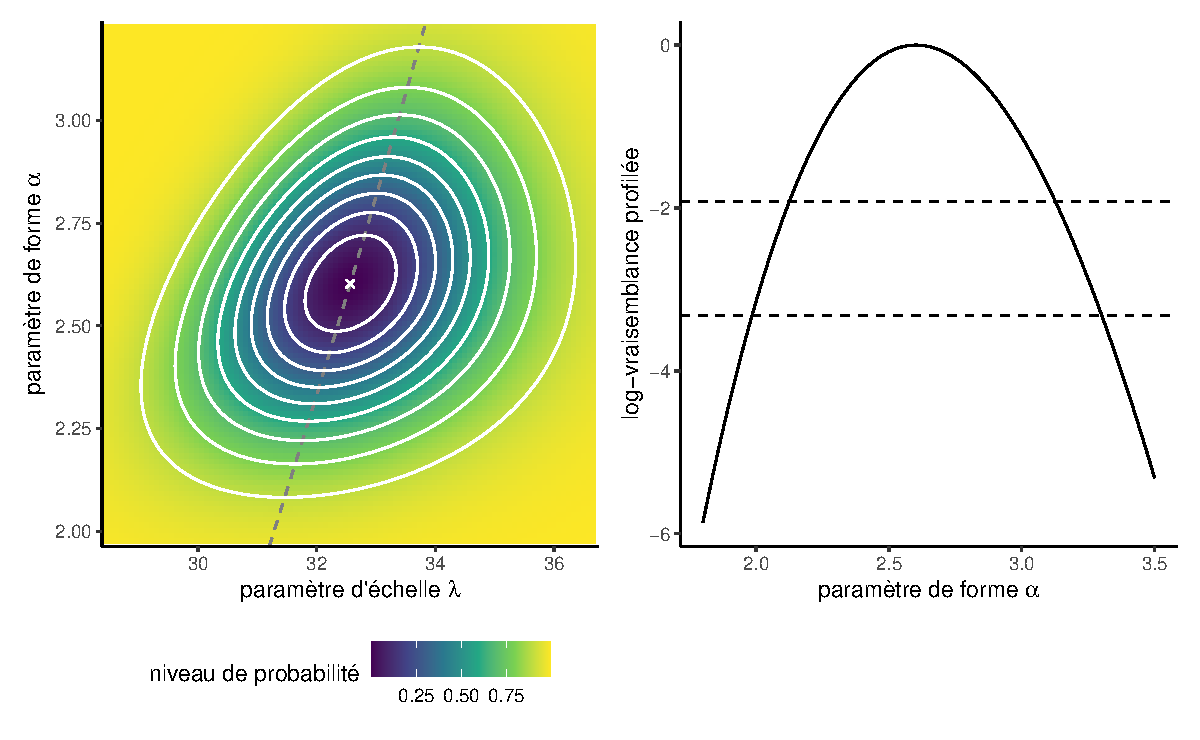
\includegraphics[width=0.85\textwidth,height=\textheight]{vraisemblance_files/figure-pdf/fig-weibull-profile-1.pdf}

}

\caption{\label{fig-weibull-profile}Log-vraisemblance profilée pour
\(\alpha\), représentée par un trait gris traitillé (gauche) et par une
coupe transversale (droite). Le panneau de gauche montre la surface de
log-vraisemblance pour le modèle de Weibull avec des régions de
confiance de 10\%, 20\%, \ldots, 90\% du rapport de vraisemblance
(courbes de contour blanches). Les valeurs de log vraisemblance les plus
élevées sont indiquées par des couleurs plus foncées, et la valeur des
estimations du maximum de vraisemblance par une croix. La vraisemblance
profilée du panneau de droite a été décalée verticalement pour que sa
valeur maximale soit zéro; les lignes horizontales traitillées indiquent
les valeurs pour les intervalles de confiance à 95\% et 99\%.}

\end{figure}%

La statistique de Wald \(W\) est la plus courante. Les intervalles de
confiance bilatéraux de niveau \((1-\alpha)\) de Wald pour les
paramètres de \(\boldsymbol{\theta}\), où pour \(\theta_j\)
\((j=1, \ldots, p)\), \begin{align*}
\widehat{\theta}_j \pm \mathfrak{z}_{1-\alpha/2}\mathrm{se}(\widehat{\theta}_j),
\end{align*} avec \(\mathfrak{z}_{1-\alpha/2}\) le quantile
\(1-\alpha/2\) d'une loi normale standard. Pour un intervalle à 95\%, le
\(0.975\) quantile vaut \(\mathfrak{z}_{0.975}=1.96.\) Les intervalles
de confiance de Wald bilatéraux sont, par construction, symmétriques.
Parfois, cela donne des valeurs impossibles (par exemple, une variance
négative).

\begin{example}[Test de Wald pour comparer les modèles Weibull et
exponentiel]\protect\hypertarget{exm-weibull-exponentiel-sousmodele}{}\label{exm-weibull-exponentiel-sousmodele}

Nous pouvons tester si la loi exponentielle est une simplification
adéquate de la loi de Weibull en imposant la restriction
\(\mathscr{H}_0: \alpha=1\). Nous comparons les statistiques de Wald
\(W\) à un \(\chi^2_1\). Puisque \(\alpha\) est un paramètre de la loi
Weibull, nous avons les erreurs-type gratuitement.

\begin{Shaded}
\begin{Highlighting}[]
\CommentTok{\# Calculer la statistique de Wald}
\NormalTok{wald\_exp }\OtherTok{\textless{}{-}}\NormalTok{ (mle\_weibull[}\DecValTok{2}\NormalTok{] }\SpecialCharTok{{-}} \DecValTok{1}\NormalTok{)}\SpecialCharTok{/}\NormalTok{se\_weibull[}\DecValTok{2}\NormalTok{]}
\CommentTok{\# Calculer la valeur{-}p}
\FunctionTok{pchisq}\NormalTok{(wald\_exp}\SpecialCharTok{\^{}}\DecValTok{2}\NormalTok{, }\AttributeTok{df =} \DecValTok{1}\NormalTok{, }\AttributeTok{lower.tail =} \ConstantTok{FALSE}\NormalTok{)}
\CommentTok{\#\textgreater{} [1] 3.61e{-}10}
\CommentTok{\# valeur{-}p inférieure à 5\%, rejet de l\textquotesingle{}hypothèse nulle}
\CommentTok{\# Intervalles de confiance de niveau 95\%}
\NormalTok{mle\_weibull[}\DecValTok{2}\NormalTok{] }\SpecialCharTok{+} \FunctionTok{qnorm}\NormalTok{(}\FunctionTok{c}\NormalTok{(}\FloatTok{0.025}\NormalTok{, }\FloatTok{0.975}\NormalTok{))}\SpecialCharTok{*}\NormalTok{se\_weibull[}\DecValTok{2}\NormalTok{]}
\CommentTok{\#\textgreater{} [1] 2.1 3.1}
\CommentTok{\# La valeur 1 n\textquotesingle{}appartient pas à l\textquotesingle{}intervalle, rejeter H0}
\end{Highlighting}
\end{Shaded}

Nous rejetons l'hypothèse nulle, ce qui signifie que le sous-modèle
exponentiel n'est pas une simplification adéquate du modèle de Weibull
\((\alpha \neq 1\)).

Nous pouvons également vérifier l'ajustement des deux modèles à l'aide
d'un diagramme quantile-quantile (cf.
Définition~\ref{def-diagramme-qq}). Il ressort de
Figure~\ref{fig-qqplots-weibull-exp} que le modèle exponentiel surestime
les temps d'attente les plus importants, dont la dispersion dans
l'échantillon est inférieure à celle impliquée par le modèle. En
revanche, la ligne droite presque parfaite pour le modèle de Weibull
dans le panneau de droite de Figure~\ref{fig-qqplots-weibull-exp}
suggère que l'ajustement du modèle est adéquat.

\begin{figure}[ht!]

\centering{

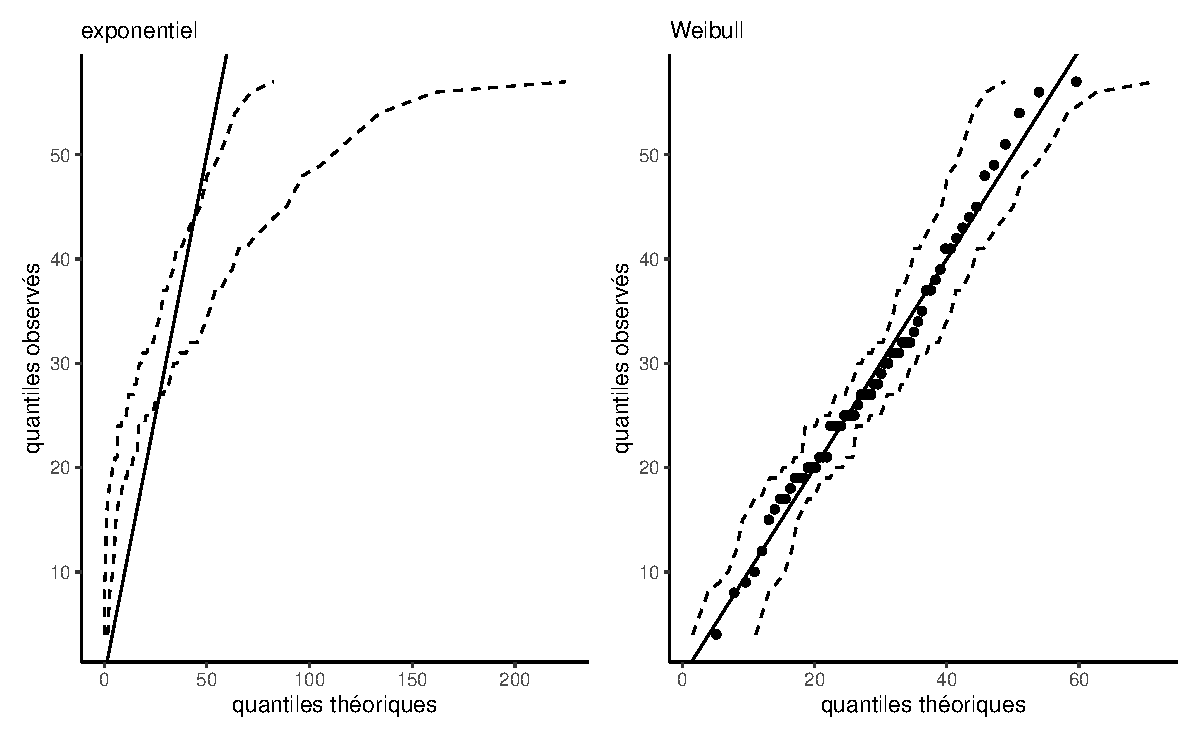
\includegraphics[width=0.85\textwidth,height=\textheight]{vraisemblance_files/figure-pdf/fig-qqplots-weibull-exp-1.pdf}

}

\caption{\label{fig-qqplots-weibull-exp}Diagrammes quantile-quantile des
modèles exponentiel (gauche) et Weibull (droite) avec intervalles de
confiance ponctuels à 95\% obtenus par autoamorçage.}

\end{figure}%

\end{example}

\begin{refremark}[Absence d'invariance des intervalles de confiance de
Wald]
Puisque les erreurs-types de paramètres dépendent de la paramétrisation,
les intervalles de confiance de Wald ne sont pas invariants à ces
transformations. Par exemple, si on veut des intervalles de confiance
pour une fonction \(g(\boldsymbol{\theta})\) qui n'est pas linéaire,
alors en général.
\(\mathsf{IC}_{W}\{g(\theta)\} \neq g\{\mathsf{IC}_{W}(\theta)\}.\)

Par exemple, considérons le modèle exponentiel. Nous pouvons inverser la
statistique du test de Wald pour obtenir un intervalle de confiance
symétrique à 95\% pour \(\phi = g(\lambda) = \exp(-60/\lambda),\) \$
{[}0.061,\$ \(0.191].\) Si nous devions naïvement transformer
l'intervalle de confiance pour \(\lambda\) en un pour \(\phi\) en
appliquant la fonction \(g(\cdot)\) à chaque borne, nous obtiendrions
plutôt \([0.063,\) \(0.19],\) Bien que la différence soit minime ici,
cela met en évidence l'invariance. L'approximation gaussienne qui
sous-tend le test de Wald est fiable si la loi d'échantillonnage de la
vraisemblance est presque quadratique, ce qui se produit lorsque la
fonction de vraisemblance est à peu près symétrique de part et d'autre
de l'estimateur du maximum de vraisemblance.

\label{rem-invariance-wald-intervalle}

\end{refremark}

Le test du rapport de vraisemblance est invariant par rapport aux
reparamétrages préservant les intérêts, de sorte que la statistique de
test pour \(\mathscr{H}_0: \phi=\phi_0\) et
\(\mathscr{H}_0: \lambda = -60/\ln(\phi_0)\) est la même. Les
intervalles de confiance de Wald peuvent être comparées à celles
(meilleures) obtenues à l'aide du test du rapport de vraisemblance. Ces
dernières sont obtenues par une recherche numérique des limites de
\begin{align*}
\left\{\theta: 2\{\ell(\widehat{\boldsymbol{\theta}}) - \ell(\boldsymbol{\theta})\} \leq \chi^2_p(1-\alpha)\right\},
\end{align*} où \(\chi^2_p(1-\alpha)\) est le quantile de niveau
\((1-\alpha)\) de la loi \(\chi^2_p\). De tels intervalles, pour
\(\alpha = 0.1, \ldots, 0.9\), sont tracés sur la
Figure~\ref{fig-weibull-profile} (courbes de contour). Si
\(\boldsymbol{\theta}\) est un \(p\)-vecteur \((p> 1)\), alors les
intervalles de confiance pour \(\theta_i\) sont dérivés à partir de la
vraisemblance profilée. Les intervalles de confiance basés sur la
statistique du rapport de vraisemblance sont \textbf{invariants aux
reparamétrages}, donc
\(\mathsf{IC}_{R}\{g(\theta)\} = g\{\mathsf{IC}_{R}(\theta)\}.\) Comme
la vraisemblance est nulle si la valeur d'un paramètre se situe en
dehors de l'espace des paramètres \(\boldsymbol{\Theta}\), les
intervalles n'incluent que les valeurs plausibles de \(\theta.\) En
général, les intervalles sont asymétriques et présentent de meilleures
taux de couverture.

\begin{Shaded}
\begin{Highlighting}[]
\CommentTok{\# Log vraisemblance exponentielle}
\NormalTok{ll\_exp }\OtherTok{\textless{}{-}} \ControlFlowTok{function}\NormalTok{(lambda) \{}
  \FunctionTok{sum}\NormalTok{(}\FunctionTok{dexp}\NormalTok{(attente, }\AttributeTok{rate =} \DecValTok{1} \SpecialCharTok{/}\NormalTok{ lambda, }\AttributeTok{log =} \ConstantTok{TRUE}\NormalTok{))}
\NormalTok{\}}
\CommentTok{\# EMV du paramètre d\textquotesingle{}échelle}
\NormalTok{lambda\_hat }\OtherTok{\textless{}{-}} \FunctionTok{mean}\NormalTok{(attente)}
\CommentTok{\# Recherche des zéros de la fonction pour obtenir}
\CommentTok{\# les limites des intervalles de confiance}
\NormalTok{lrt\_lb }\OtherTok{\textless{}{-}} \FunctionTok{uniroot}\NormalTok{(}
  \CommentTok{\# borne inférieure, en utilisant l\textquotesingle{}EMV}
  \AttributeTok{f =} \ControlFlowTok{function}\NormalTok{(r) \{}
    \DecValTok{2} \SpecialCharTok{*}\NormalTok{ (}\FunctionTok{ll\_exp}\NormalTok{(lambda\_hat) }\SpecialCharTok{{-}} \FunctionTok{ll\_exp}\NormalTok{(r)) }\SpecialCharTok{{-}} \FunctionTok{qchisq}\NormalTok{(}\FloatTok{0.95}\NormalTok{, }\DecValTok{1}\NormalTok{)}
\NormalTok{  \},}
  \AttributeTok{interval =} \FunctionTok{c}\NormalTok{(}\FloatTok{0.5} \SpecialCharTok{*} \FunctionTok{min}\NormalTok{(attente), lambda\_hat)}
\NormalTok{)}\SpecialCharTok{$}\NormalTok{root}
\NormalTok{lrt\_ub }\OtherTok{\textless{}{-}} \FunctionTok{uniroot}\NormalTok{(}
  \CommentTok{\# borne supérieure}
  \AttributeTok{f =} \ControlFlowTok{function}\NormalTok{(r) \{}
    \DecValTok{2} \SpecialCharTok{*}\NormalTok{ (}\FunctionTok{ll\_exp}\NormalTok{(lambda\_hat) }\SpecialCharTok{{-}} \FunctionTok{ll\_exp}\NormalTok{(r)) }\SpecialCharTok{{-}} \FunctionTok{qchisq}\NormalTok{(}\FloatTok{0.95}\NormalTok{, }\DecValTok{1}\NormalTok{)}
\NormalTok{  \},}
  \AttributeTok{interval =} \FunctionTok{c}\NormalTok{(lambda\_hat, }\DecValTok{2} \SpecialCharTok{*} \FunctionTok{max}\NormalTok{(attente))}
\NormalTok{)}\SpecialCharTok{$}\NormalTok{root}
\end{Highlighting}
\end{Shaded}

L'intervalle de confiance à 95\% de la statistique du rapport de
vraisemblance pour \(\lambda\) peut être trouvé en utilisant un
algorithme de recherche linéaire: l'intervalle de confiance à 95\% pour
\(\lambda\) est \(\mathsf{IC}_R(\lambda)[22.784,37.515].\) Par
invariance, l'intervalle de confiance à 95\% pour \(\phi\) est
\(\mathsf{IC}_R(\phi) = [0.072, 0.202] = g\{\mathsf{IC}_R(\lambda)\}.\)

\section{Vraisemblance profilée}\label{vraisemblance-profiluxe9e}

Parfois, nous pouvons vouloir effectuer des tests d'hypothèse ou dériver
des intervalles de confiance pour un sous-ensemble spécifique des
paramètres du modèle, ou une transformation de ces derniers. Dans ce
cas, l'hypothèse nulle ne restreint qu'une partie de l'espace et les
autres paramètres, dits de nuisance, ne sont pas spécifiés --- la
question est alors de savoir quelles valeurs utiliser pour la
comparaison avec le modèle complet. Il s'avère que les valeurs qui
maximisent la log-vraisemblance contrainte sont celles que l'on doit
utiliser pour le test, et la fonction particulière dans laquelle ces
paramètres de nuisance sont intégrés est appelée vraisemblance profilée.

\begin{definition}[Log-vraisemblance
profilée]\protect\hypertarget{def-logvraisemblance}{}\label{def-logvraisemblance}

Soit un modèle paramétrique avec log-vraisemblance
\(\ell(\boldsymbol{\theta})\), dont le vecteur de paramètres de
dimension \(p\)
\(\boldsymbol{\theta}=(\boldsymbol{\psi}, \boldsymbol{\varphi})\) peut
être séparé en un sous-vecteur de longueur \(q\) contenant les
paramètres d'intérêts, disons \(\boldsymbol{\psi}\) et un sous-vecteur
de longueur \((p-q)\) contenant les paramètres de nuisance
\(\boldsymbol{\varphi}.\)

La log-vraisemblance profilée \(\ell_{\mathsf{p}}\) est une fonction de
\(\boldsymbol{\psi}\) qui est obtenue en maximisant la log-vraisemblance
ponctuellement à chaque valeur fixe \(\boldsymbol{\psi}_0\) sur le
vecteur de nuisance \(\boldsymbol{\varphi}_{\psi_0},\) \begin{align*}
\ell_{\mathsf{p}}(\boldsymbol{\psi})=\max_{\boldsymbol{\varphi}}\ell(\boldsymbol{\psi}, \boldsymbol{\varphi})=\ell(\boldsymbol{\psi}, \widehat{\boldsymbol{\varphi}}_{\boldsymbol{\psi}}).
\end{align*}

\end{definition}

\begin{example}[Log-vraisemblance profilée pour le paramètre de forme
d'une loi
Weibull]\protect\hypertarget{exm-profile-alpha-weibull}{}\label{exm-profile-alpha-weibull}

Considérons le paramètre de forme \(\psi \equiv\alpha\) comme paramètre
d'intérêt, et le paramètre d'échelle \(\varphi\equiv\lambda\) comme
paramètre de nuisance. En utilisant le gradient dérivé dans
l'Exemple~\ref{exm-weibull-emv}, nous constatons que la valeur de
l'échelle qui maximise la log-vraisemblance pour un \(\alpha\) donné est
\begin{align*}
\widehat{\lambda}_\alpha = \left( \frac{1}{n}\sum_{i=1}^n y_i^\alpha\right)^{1/\alpha}.
\end{align*} Si on substitue cette valeur dans la log-vraisemblance, on
obtient une fonction de \(\alpha\) uniquement, ce qui réduit également
le problème d'optimisation pour les EMV d'une loi Weibull à une
recherche linéaire le long de \(\ell_{\mathsf{p}}(\alpha)\). Le panneau
de gauche de Figure~\ref{fig-weibull-profile} montre la crête le long de
la direction de \(\alpha\) correspondant à la surface de
log-vraisemblance. Si l'on considère ces courbes de niveau comme celles
d'une carte topographique, la log-vraisemblance profilée correspond dans
ce cas à une marche le long de la crête des deux montagnes dans la
direction \(\psi\), le panneau de droite montrant le gain/la perte
d'altitude. Le profil d'élévation correspondant à droite de
Figure~\ref{fig-weibull-profile} avec les points de coupure pour les
intervalles de confiance basés sur le rapport de vraisemblance\textless.
Nous devrions obtenir numériquement, à l'aide d'un algorithme de
recherche lin/aire, les limites de l'intervalle de confiance de part et
d'autre de \(\widehat{\alpha}\), mais il est clair que \(\alpha=1\)
n'est pas dans l'intervalle de 99\%.

\begin{Shaded}
\begin{Highlighting}[]
\CommentTok{\# EMV conditionnels de lambda pour alpha donné}
\NormalTok{lambda\_alpha }\OtherTok{\textless{}{-}} \ControlFlowTok{function}\NormalTok{(alpha, }\AttributeTok{y =}\NormalTok{ attente) \{}
\NormalTok{  (}\FunctionTok{mean}\NormalTok{(y}\SpecialCharTok{\^{}}\NormalTok{alpha))}\SpecialCharTok{\^{}}\NormalTok{(}\DecValTok{1} \SpecialCharTok{/}\NormalTok{ alpha)}
\NormalTok{\}}
\CommentTok{\# Log vraisemblance profilée pour alpha}
\NormalTok{prof\_alpha\_weibull }\OtherTok{\textless{}{-}} \ControlFlowTok{function}\NormalTok{(par, }\AttributeTok{y =}\NormalTok{ attente) \{}
  \FunctionTok{sapply}\NormalTok{(par, }\ControlFlowTok{function}\NormalTok{(a) \{}
    \FunctionTok{nll\_weibull}\NormalTok{(}\AttributeTok{pars =} \FunctionTok{c}\NormalTok{(}\FunctionTok{lambda\_alpha}\NormalTok{(a), a), }\AttributeTok{y =}\NormalTok{ y)}
\NormalTok{  \})}
\NormalTok{\}}
\end{Highlighting}
\end{Shaded}

\end{example}

\begin{example}[Log-vraisemblance profilée pour l'espérance d'une loi
Weibull]\protect\hypertarget{exm-profile-mean-weibull}{}\label{exm-profile-mean-weibull}

Nous pouvons également utiliser l'optimisation numérique pour calculer
la log-vraisemblance profilée d'une fonction des paramètres. Supposons
que nous soyons intéressés par le temps moyen d'attente théorique. Selon
le modèle Weibull, cette valeur est
\(\mu = \mathsf{E}(Y) = \lambda\Gamma(1+1/\alpha)\). À cet effet, nous
reparamétrons le modèle en termes de \((\mu, \alpha)\), où
\(\lambda=\mu/\Gamma(1+1/\alpha)\). Nous créons ensuite une fonction qui
optimise la log-vraisemblance pour une valeur fixe de \(\mu\), puis
renvoie \(\widehat{\alpha}_{\mu}\), \(\mu\) et
\(\ell_{\mathrm{p}}(\mu)\).

Pour obtenir les intervalles de confiance d'un paramètre scalaire, il
existe une astuce qui permet de s'en tirer avec une évaluation sommaire,
pour autant que la log-vraisemblance profilée soit relativement lisse.
Nous calculons la racine directionnelle du rapport de vraisemblance,
\(r(\psi) = \mathrm{sign}(\psi - \widehat{\psi})\{2\ell_{\mathrm{p}}(\widehat{\psi}) -2 \ell_{\mathrm{p}}(\psi)\}^{1/2}\)
sur une grille fine de valeurs de \(\psi\), puis nous ajustons une
spline de lissage, une régression avec variable réponse \(y=\psi\) et
variable explicative \(x=r(\psi)\). Nous prédisons ensuite la courbe aux
quantiles normaux \(\mathfrak{z}_{\alpha/2}\) et
\(\mathfrak{z}_{1-\alpha/2}\), et renvoyons ces valeurs sous forme
d'intervalle de confiance. La Figure~\ref{fig-profile-mu-weibull} montre
comment ces valeurs correspondent aux points de coupure sur l'échelle du
logarithme du rapport de vraisemblance, où la ligne verticale est donnée
par \(-\mathfrak{c}(1-\alpha)/2\) où \(\mathfrak{c}\) représente le
quantile d'une variable aléatoire \(\chi^2_1\).

\begin{Shaded}
\begin{Highlighting}[]
\CommentTok{\# Compute the MLE for the expected value via plug{-}in}
\NormalTok{mu\_hat }\OtherTok{\textless{}{-}}\NormalTok{ mle\_weibull[}\DecValTok{1}\NormalTok{]}\SpecialCharTok{*}\FunctionTok{gamma}\NormalTok{(}\DecValTok{1}\SpecialCharTok{+}\DecValTok{1}\SpecialCharTok{/}\NormalTok{mle\_weibull[}\DecValTok{2}\NormalTok{])}
\CommentTok{\# Create a profile function}
\NormalTok{prof\_weibull\_mu }\OtherTok{\textless{}{-}} \ControlFlowTok{function}\NormalTok{(mu)\{}
  \CommentTok{\# For given value of mu}
\NormalTok{  alpha\_mu }\OtherTok{\textless{}{-}} \ControlFlowTok{function}\NormalTok{(mu)\{ }
  \CommentTok{\# Find the profile by optimizing (line search) for fixed mu and the best alpha}
\NormalTok{     opt }\OtherTok{\textless{}{-}} \FunctionTok{optimize}\NormalTok{(}\AttributeTok{f =} \ControlFlowTok{function}\NormalTok{(alpha, mu)\{}
     \CommentTok{\# minimize the negative log likelihood}
      \FunctionTok{nll\_weibull}\NormalTok{(}\FunctionTok{c}\NormalTok{(mu}\SpecialCharTok{/}\FunctionTok{gamma}\NormalTok{(}\DecValTok{1}\SpecialCharTok{+}\DecValTok{1}\SpecialCharTok{/}\NormalTok{alpha), alpha), }\AttributeTok{y =}\NormalTok{ attente)\}, }
   \AttributeTok{mu =}\NormalTok{ mu, }
  \AttributeTok{interval =} \FunctionTok{c}\NormalTok{(}\FloatTok{0.1}\NormalTok{,}\DecValTok{10}\NormalTok{) }\CommentTok{\#search region}
\NormalTok{  )}
  \CommentTok{\# Return the value of the negative log likelihood and alpha\_mu}
  \FunctionTok{return}\NormalTok{(}\FunctionTok{c}\NormalTok{(}\AttributeTok{nll =}\NormalTok{ opt}\SpecialCharTok{$}\NormalTok{objective, }\AttributeTok{alpha =}\NormalTok{ opt}\SpecialCharTok{$}\NormalTok{minimum))}
\NormalTok{  \}}
  \CommentTok{\# Create a data frame with mu and the other parameters}
  \FunctionTok{data.frame}\NormalTok{(}\AttributeTok{mu =}\NormalTok{ mu, }\FunctionTok{t}\NormalTok{(}\FunctionTok{sapply}\NormalTok{(mu, }\ControlFlowTok{function}\NormalTok{(m)\{}\FunctionTok{alpha\_mu}\NormalTok{(m)\})))}
\NormalTok{\}}
\CommentTok{\# Create a data frame with the profile  }
\NormalTok{prof }\OtherTok{\textless{}{-}} \FunctionTok{prof\_weibull\_mu}\NormalTok{(}\FunctionTok{seq}\NormalTok{(}\DecValTok{22}\NormalTok{, }\DecValTok{35}\NormalTok{, }\AttributeTok{length.out =} \DecValTok{101}\NormalTok{L))}
\CommentTok{\# Compute signed likelihood root r}
\NormalTok{prof}\SpecialCharTok{$}\NormalTok{r }\OtherTok{\textless{}{-}} \FunctionTok{sign}\NormalTok{(prof}\SpecialCharTok{$}\NormalTok{mu }\SpecialCharTok{{-}}\NormalTok{ mu\_hat)}\SpecialCharTok{*}\FunctionTok{sqrt}\NormalTok{(}\DecValTok{2}\SpecialCharTok{*}\NormalTok{(prof}\SpecialCharTok{$}\NormalTok{nll }\SpecialCharTok{{-}}\NormalTok{ opt\_weibull}\SpecialCharTok{$}\NormalTok{value))}

\CommentTok{\# Trick: fit a spline to obtain the predictions with mu as a function of r}
\CommentTok{\# Then use this to predict the value at which we intersect the normal quantiles}
\NormalTok{fit.r }\OtherTok{\textless{}{-}}\NormalTok{ stats}\SpecialCharTok{::}\FunctionTok{smooth.spline}\NormalTok{(}\AttributeTok{x =} \FunctionTok{cbind}\NormalTok{(prof}\SpecialCharTok{$}\NormalTok{r, prof}\SpecialCharTok{$}\NormalTok{mu), }\AttributeTok{cv =} \ConstantTok{FALSE}\NormalTok{)}
\NormalTok{pr }\OtherTok{\textless{}{-}} \FunctionTok{predict}\NormalTok{(fit.r, }\FunctionTok{qnorm}\NormalTok{(}\FunctionTok{c}\NormalTok{(}\FloatTok{0.025}\NormalTok{, }\FloatTok{0.975}\NormalTok{)))}\SpecialCharTok{$}\NormalTok{y}
\CommentTok{\# Plot the signed likelihood root {-} near linear indicates quadratic}
\NormalTok{g1 }\OtherTok{\textless{}{-}} \FunctionTok{ggplot}\NormalTok{(}\AttributeTok{data =}\NormalTok{ prof,}
     \AttributeTok{mapping =} \FunctionTok{aes}\NormalTok{(}\AttributeTok{x =}\NormalTok{ mu, }\AttributeTok{y =}\NormalTok{ r)) }\SpecialCharTok{+}
  \FunctionTok{geom\_abline}\NormalTok{(}\AttributeTok{intercept =} \DecValTok{0}\NormalTok{, }\AttributeTok{slope =} \DecValTok{1}\NormalTok{) }\SpecialCharTok{+}
  \FunctionTok{geom\_line}\NormalTok{() }\SpecialCharTok{+} 
  \FunctionTok{geom\_hline}\NormalTok{(}\AttributeTok{yintercept =} \FunctionTok{qnorm}\NormalTok{(}\FloatTok{0.025}\NormalTok{, }\FloatTok{0.975}\NormalTok{),}
            \AttributeTok{linetype =} \StringTok{"dashed"}\NormalTok{) }\SpecialCharTok{+} 
  \FunctionTok{labs}\NormalTok{(}\AttributeTok{x =} \FunctionTok{expression}\NormalTok{(}\FunctionTok{paste}\NormalTok{(}\StringTok{"espérance "}\NormalTok{, mu)),}
       \AttributeTok{y =} \StringTok{"racine directionnelle de vraisemblance"}\NormalTok{)}
\CommentTok{\# Create a plot of the profile}
\NormalTok{g2 }\OtherTok{\textless{}{-}} \FunctionTok{ggplot}\NormalTok{(}\AttributeTok{data =}\NormalTok{ prof,}
       \AttributeTok{mapping =} \FunctionTok{aes}\NormalTok{(}\AttributeTok{x =}\NormalTok{ mu, }\AttributeTok{y =}\NormalTok{ opt\_weibull}\SpecialCharTok{$}\NormalTok{value }\SpecialCharTok{{-}}\NormalTok{ nll)) }\SpecialCharTok{+} 
  \FunctionTok{geom\_line}\NormalTok{() }\SpecialCharTok{+}
  \FunctionTok{geom\_hline}\NormalTok{(}\AttributeTok{yintercept =} \SpecialCharTok{{-}}\FunctionTok{qchisq}\NormalTok{(}\FunctionTok{c}\NormalTok{(}\FloatTok{0.95}\NormalTok{), }\AttributeTok{df =} \DecValTok{1}\NormalTok{)}\SpecialCharTok{/}\DecValTok{2}\NormalTok{,}
             \AttributeTok{linetype =} \StringTok{"dashed"}\NormalTok{) }\SpecialCharTok{+}
  \FunctionTok{geom\_vline}\NormalTok{(}\AttributeTok{linetype =} \StringTok{"dotted"}\NormalTok{,}
  \AttributeTok{xintercept =}\NormalTok{ pr) }\SpecialCharTok{+} 
  \FunctionTok{labs}\NormalTok{(}\AttributeTok{x =} \FunctionTok{expression}\NormalTok{(}\FunctionTok{paste}\NormalTok{(}\StringTok{"espérance "}\NormalTok{, mu)),}
       \AttributeTok{y =} \StringTok{"log vraisemblance profilée"}\NormalTok{)}

\NormalTok{g1 }\SpecialCharTok{+}\NormalTok{ g2}
\end{Highlighting}
\end{Shaded}

\begin{figure}[ht!]

\centering{

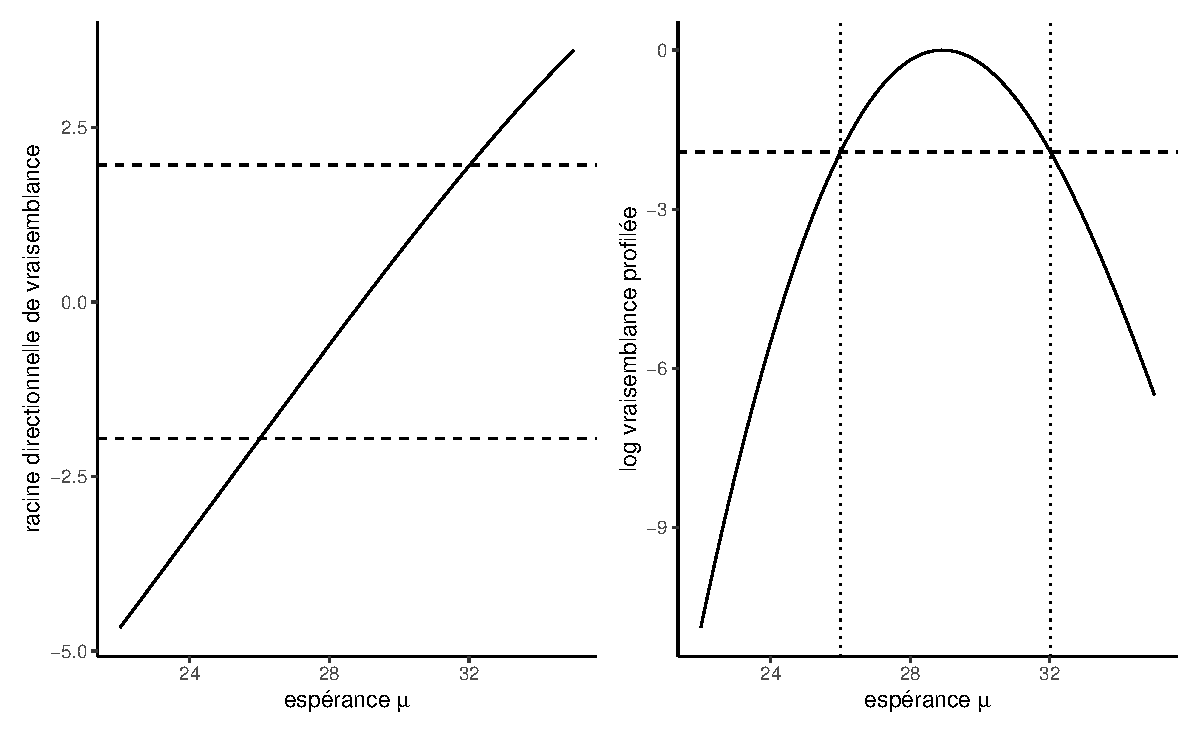
\includegraphics[width=0.85\textwidth,height=\textheight]{vraisemblance_files/figure-pdf/fig-profile-mu-weibull-1.pdf}

}

\caption{\label{fig-profile-mu-weibull}Racine directionnelle du rapport
de vraisemblance (gauche) et log vraisemblance profilée (droite) en
fonction de l'espérance \(\mu\) pour un modèle Weibull.}

\end{figure}%

\end{example}

L'estimateur du maximum de vraisemblance du profil se comporte comme une
vraisemblance normale pour la plupart des quantités d'intérêt et nous
pouvons dériver des statistiques de test et des intervalles de confiance
de la manière habituelle. Un exemple célèbre de profil de vraisemblance
est la fonction de risque proportionnel de Cox couvert dans le
\hyperref[survie]{chapitre 7}.

\begin{example}[Transformation de
Box--Cox]\protect\hypertarget{exm-boxcox}{}\label{exm-boxcox}

Parfois, le postulat de normalité de l'erreur dans une régression
linéaire ne tient pas. Si les données sont strictement positives, on
peut envisager une transformation de Box-Cox, \begin{align*}
y(\lambda)= \begin{cases}
(y^{\lambda}-1)/\lambda, & \lambda \neq 0\\
\ln(y), & \lambda=0.
\end{cases}
\end{align*}

Si on postule que
\(\boldsymbol{Y}(\lambda) \sim \mathsf{normale}(\mathbf{X}\boldsymbol{\beta}, \sigma^2 \mathbf{I}_n)\),
alors la log-vraisemblance s'écrit \begin{align*}
L(\lambda, \boldsymbol{\beta}, \sigma; \boldsymbol{y}, \mathbf{X}) &= (2\pi\sigma^2)^{-n/2} J(\lambda, \boldsymbol{y}) \times\\& \quad \exp \left[ - \frac{1}{2\sigma^2}\{\boldsymbol{y}(\lambda) - \mathbf{X}\boldsymbol{\beta}\}^\top\{\boldsymbol{y}(\lambda) - \mathbf{X}\boldsymbol{\beta}\}\right],
\end{align*} où \(J\) dénote le jacobien de la transformation de
Box--Cox, \(J(\lambda, \boldsymbol{y})=\prod_{i=1}^n y_i^{\lambda-1}\).
Pour chaque valeur de \(\lambda\), l'estimateur du maximum de
vraisemblance est le même que celle de la régression linéaire, mais où
\(\boldsymbol{y}\) est remplacée par \(\boldsymbol{y}(\lambda)\), soit
\(\widehat{\boldsymbol{\beta}}_\lambda = (\mathbf{X}^\top\mathbf{X})^{-1}\mathbf{X}^\top \boldsymbol{y}(\lambda)\)
and
\(\widehat{\sigma}^2_\lambda = n^{-1}\{ \boldsymbol{y}(\lambda) - \mathbf{X}\widehat{\boldsymbol{\beta}}_\lambda\}^\top\{ \boldsymbol{y}(\lambda) - \mathbf{X}\widehat{\boldsymbol{\beta}}_\lambda\}\).

La log-vraisemblance profilée est donc \begin{align*}
\ell_{\mathsf{p}}(\lambda) = -\frac{n}{2}\ln(2\pi \widehat{\sigma}^2_\lambda) - \frac{n}{2} + (\lambda - 1)\sum_{i=1}^n \ln(y_i)
\end{align*} L'estimateur du maximum de vraisemblance profilée est la
valeur \(\lambda\) qui minimise la somme des carrés des résidus du
modèle linéaire avec \(\boldsymbol{y}(\lambda)\) comme réponse.

La transformation de Box--Cox n'est pas une solution miracle et doit
être réservée aux cas où la transformation réduit l'hétéroscédasticité
(variance inégale) ou crée une relation linéaire entre les explications
et la réponse. La théorie fournit une explication convaincante des
données avec, par exemple, la fonction de production Cobb-Douglas
utilisée en économie qui peut être linéarisée par une transformation
logarithmique. Plutôt que de choisir une transformation \emph{ad hoc},
on pourrait choisir une transformation logarithmique si la valeur 0\$
est incluse dans l'intervalle de confiance à 95\%, car cela améliore
l'interprétabilité.

\end{example}

\section{Critères d'information}\label{crituxe8res-dinformation}

La vraisemblance peut également servir d'élément de base pour la
comparaison des modèles : plus \(\ell(\boldsymbol{\widehat{\theta}})\)
est grand, meilleure est l'adéquation. Cependant, la vraisemblance ne
tient pas compte de la complexité du modèle dans le sens où des modèles
plus complexes avec plus de paramètres conduisent à une vraisemblance
plus élevée. Cela ne pose pas de problème pour la comparaison de modèles
emboîtés à l'aide du test du rapport de vraisemblance, car nous ne
tenons compte que de l'amélioration relative de l'adéquation. Il existe
un risque de \textbf{surajustement} si l'on ne tient compte que de la
vraisemblance d'un modèle.

Les critères d'information combinent la log vraisemblance, qui mesure
l'adéquation du modèle aux données, avec une pénalité pour le nombre de
paramètres. Les plus fréquents sont les critères d'information d'Akaike
(AIC) et bayésien (BIC), \begin{align*}
\mathsf{AIC}&=-2\ell(\widehat{\boldsymbol{\theta}})+2p \\
\mathsf{BIC}&=-2\ell(\widehat{\boldsymbol{\theta}})+p\ln(n),
\end{align*} où \(p\) dénote le nombre de paramètres du modèle. Le plus
petit la valeur du critère d'information, le meilleur le modèle.

Notez que les critères d'information ne constituent pas des tests
d'hypothèse formels sur les paramètres, mais qu'ils peuvent être
utilisés pour comparer des modèles non imbriqués (mais ils sont alors
très imprécis!) Ces outils fonctionnent sous des conditions de
régularité et les critères d'information estimés sont assez bruyants, de
sorte que les comparaisons pour les modèles non emboîtés sont
hasardeuses bien que populaires. Si nous voulons comparer la
vraisemblance de différents modèles de probabilité, nous devons nous
assurer qu'ils incluent une constante de normalisation\footnote{Les
  logiciels enlèvent parfois les termes ou constantes qui ne sont pas
  des fonctions des paramètres.}. Le \(\mathsf{BIC}\) est plus strict
que le \(\mathsf{AIC}\), car sa pénalité augmente avec la taille de
l'échantillon, ce qui permet de sélectionner des modèles plus
parsimonieux. Le \(\mathsf{BIC}\) est un critère \textbf{convergent}, ce
qui signifie qu'il choisira le vrai modèle parmi un ensemble de modèles
avec une probabilité de 1 lorsque \(n \to \infty\) si ce dernier fait
partie du catalogue de modèles à comparer. En pratique, cela présente
peu d'intérêt si l'on suppose que tous les modèles sont des
approximations de la réalité (il est peu probable que le vrai modèle
soit inclus dans ceux que nous considérons). Pour sa part,
\(\mathsf{AIC}\) sélectionne souvent des modèles trop compliqués dans
les grands échantillons, alors que \(\mathsf{BIC}\) choisit des modèles
trop simples.

Une mise en garde s'impose: s'il est possible de comparer des modèles de
régression non emboîtés à l'aide de critères d'information, ceux-ci ne
peuvent être utilisés que lorsque la variable de réponse est la même.
Vous pouvez comparer une régression de Poisson avec une régression
linéaire pour une réponse \(Y\) en utilisant des critères d'information
à condition d'inclure toutes les constantes de normalisation dans votre
modèle. Les logiciels omettent souvent les termes constants; cela n'a
pas d'impact lorsque vous comparez des modèles avec les mêmes facteurs
constants, mais cela a de l'importance lorsque ceux-ci diffèrent.
Cependant, \textbf{on ne peut pas} les comparer à un modèle log-linéaire
avec une réponse \(\ln(Y)\). Les comparaisons entre les modèles
log-linéaires et linéaires ne sont valables que si vous utilisez la
vraisemblance de Box--Cox, car elle inclut le jacobien de la
transformation.

\bookmarksetup{startatroot}

\chapter{Régression linéaire}\label{regression-lineaire}

\section{Introduction}\label{introduction}

Le modèle de régression linéaire, ou modèle linéaire, est l'un des
outils les plus polyvalents pour l'inférence statistique. La régression
linéaire est principalement utilisée pour évaluer les effets des
variables explicatives (souvent l'effet d'une manipulation ou d'un
traitement dans un cadre expérimental) sur la moyenne d'une variable
réponse continue, ou pour la prédiction. Un modèle linéaire est un
modèle qui décrit la moyenne d'une \textbf{variable réponse} continue
\(Y_i\) d'un échantillon aléatoire de taille \(n\) comme
\textbf{fonction linéaire} des \textbf{variables explicatives}
(également appelés prédicteurs, régresseurs ou covariables)
\(X_1, \ldots, X_p\).

Dénotons par \(Y_i\) la valeur de \(Y\) pour le sujet \(i\), et
\(X_{ij}\) la valeur de la \(j\)e variable explicative du sujet \(i\).
\begin{align}
\underset{\text{moyenne conditionnelle}}{\mathsf{E}(Y_i \mid \boldsymbol{X}_i=\boldsymbol{x}_i)}=\mu_i=\underset{\substack{\text{combinaison linéaire (somme pondérée)}\\ \text{de variables explicatives}}}{\beta_0 + \beta_1x_{i1} + \cdots + \beta_p x_{ip}}\equiv \mathbf{x}_i\boldsymbol{\beta}.
\end{align} où \(\mathbf{x}_i = (1, x_{i1}, \ldots, x_{ip})\) est un
vecteur ligne de taille \((p+1)\) contenant les variables explicatives
de l'observation \(i\) et
\(\boldsymbol{\beta} = (\beta_0, \ldots, \beta_p)^\top\) est un vecteur
colonne de longueur \(p+1\) contenant les coefficients de la moyenne. Le
fait que la moyenne est conditionnelle aux valeurs de \(\mathbf{X}\)
implique simplement que l'on considère les régresseurs comme constant,
ou connus à l'avance. Les coefficients \(\boldsymbol{\beta}\) sont les
mêmes pour toutes les observations, mais le vecteurs de variables
explicatives \(\mathbf{x}_i\) peut différer d'une observation à l'autre.
Le modèle est \textbf{linéaire} en \(\beta_0, \ldots, \beta_p\), pas
nécessairement dans les variables explicatives.

Pour simplifier la notation, nous regroupons les observations dans un
vecteur \(n\) \(\boldsymbol{Y}\) et les explications dans une matrice
\(n \times (p+1)\) \(\mathbf{X}\) en concaténant une colonne de uns et
les vecteurs de colonnes \(p\)
\(\boldsymbol{X}_1, \ldots, \boldsymbol{X}_p\), chacun contenant les
\(n\) observations des explications respectives. La matrice
\(\mathbf{X}\) est appelée \textbf{matrice du modèle} (ou parfois
matrice de devis dans un contexte expérimental), et sa \(i\)ème ligne
est \(\mathbf{x}_i\).

En supposant que la variable réponse provient d'une famille de
localisation, nous pouvons réécrire le modèle linéaire en termes de la
moyenne plus un aléa, \begin{align*}
\underset{\text{observation}\vphantom{\mu_i}}{Y_i} = \underset{\text{moyenne } \mu_i}{\vphantom{Y_i}\mathbf{x}_i\boldsymbol{\beta}} + \underset{\text{aléa}\vphantom{\mu_i}}{\vphantom{Y_i}\varepsilon_i},
\end{align*} où \(\varepsilon_i\) est le terme spécifique à
l'observation \(i\). On assume que les aléas
\(\varepsilon_1, \ldots \varepsilon_n\) sont indépendants et
identiquement distribués, avec
\(\mathsf{E}(\varepsilon_i \mid \mathbf{x}_i) = 0\) et
\(\mathsf{Var}(\varepsilon_i \mid \mathbf{x}_i) = \sigma^2\). On fixe
l'espérance de l'aléa à zéro car on postule qu'il n'y a pas d'erreur
systématique. La variance \(\sigma^2\) sert à tenir compte du fait
qu'aucune relation linéaire exacte ne lie \(\mathbf{x}_i\) et \(Y_i\),
ou que les mesures de \(Y_i\) sont variables.

Le modèle linéaire normal ou gaussien spécifie que les réponses suivent
une loi normale, avec
\(Y_i \mid \boldsymbol{X}_i=\boldsymbol{x}_i \sim \mathsf{normale}(\mathbf{x}_i\boldsymbol{\beta}, \sigma^2)\).
La loi normale est une famille de localisation, de sorte que
\(Y \sim \mathsf{normale}(\mu, \sigma^2)\) équivaut à la décomposition
additive \(\mu + \varepsilon\) pour
\(\varepsilon \sim \mathsf{normale}(0, \sigma^2)\).

\subsection{Exemples}\label{exemples-1}

Considérons quelques exemples de jeux de données qui serviront à
illustrer les méthodes par la suite.

\begin{example}[Cohérence de descriptions de
produits]\protect\hypertarget{exm-lee-choi1}{}\label{exm-lee-choi1}

L'étude 1 de Lee et Choi (\citeproc{ref-Lee.Choi:2019}{2019}) (base de
données \texttt{LC19\_S1}, paquet \texttt{hecedsm}) considère l'impact
sur la perception d'un produit de la divergence entre la description
textuelle et l'image. Dans leur première expérience, un paquet de six
brosses à dents est vendu, mais l'image montre soit un paquet de six,
soit une seule). Les auteurs ont également mesuré la familiarité
préalable avec la marque de l'article. Les \(n=96\) participants ont été
recrutés à l'aide d'un panel en ligne. Nous pourrions ajuster un modèle
linéaire pour le score moyen d'évaluation du produit, \texttt{prodeval},
en fonction de la familiarité de la marque \texttt{familiarity}, un
nombre entier allant de 1 à 7, et une variable binaire pour le facteur
expérimental \texttt{consistency}, codé \texttt{0} pour des descriptions
d'image/texte cohérentes et \texttt{1} si elles sont incohérentes. La
matrice du modèle qui en résulte est alors de dimension \(96\times 3\).
La réponse \texttt{prodeval} est fortement discrétisée.

\begin{Shaded}
\begin{Highlighting}[]
\FunctionTok{data}\NormalTok{(LC19\_S1, }\AttributeTok{package =} \StringTok{"hecedsm"}\NormalTok{)}
\NormalTok{modmat }\OtherTok{\textless{}{-}} \FunctionTok{model.matrix}\NormalTok{( }\CommentTok{\# Matrice du modèle}
     \SpecialCharTok{\textasciitilde{}}\NormalTok{ familiarity }\SpecialCharTok{+}\NormalTok{ consistency,}
     \AttributeTok{data =}\NormalTok{ LC19\_S1)}
\FunctionTok{tail}\NormalTok{(modmat, }\AttributeTok{n =} \DecValTok{5}\NormalTok{L) }\CommentTok{\# Imprimer les premières 5 lignes}
\CommentTok{\#\textgreater{}    (Intercept) familiarity consistencyinconsistent}
\CommentTok{\#\textgreater{} 92           1           6                       1}
\CommentTok{\#\textgreater{} 93           1           4                       1}
\CommentTok{\#\textgreater{} 94           1           7                       1}
\CommentTok{\#\textgreater{} 95           1           7                       1}
\CommentTok{\#\textgreater{} 96           1           7                       1}
\FunctionTok{dim}\NormalTok{(modmat) }\CommentTok{\# dimension de la matrice du modèle}
\CommentTok{\#\textgreater{} [1] 96  3}
\end{Highlighting}
\end{Shaded}

\end{example}

\begin{example}[Méthodes d'apprentissage de compréhension de
lecture]\protect\hypertarget{exm-teaching-baumann}{}\label{exm-teaching-baumann}

La base de données \texttt{BSJ92} du paquet \texttt{hecedsm} contient
les résultats d'une expérience de Baumann, Seifert-Kessell, et Jones
(\citeproc{ref-Baumann:1992}{1992}) sur l'efficacité de différentes
stratégies de lecture sur la compréhension d'enfants.

\begin{quote}
Soixante-six élèves de quatrième année ont été assignés au hasard à l'un
des trois groupes expérimentaux suivants : (a) un groupe « Think-Aloud »
(TA), dans lequel les élèves ont appris diverses stratégies de contrôle
de la compréhension pour la lecture d'histoires (par exemple :
auto-questionnement, prédiction, relecture) par le biais de la réflexion
à haute voix; (b) un groupe lecture dirigée-activité de réflexion
(DRTA), dans lequel les élèves ont appris une stratégie de
prédiction-vérification pour lire et répondre aux histoires; ou (c) un
groupe activité de lecture dirigée (DRA), un groupe contrôle dans lequel
les élèves se sont engagés dans une lecture guidée non interactive
d'histoires.
\end{quote}

Les variables d'intérêt sont \texttt{group}, le facteur pour le groupe
expérimental, soit \texttt{DRTA}, \texttt{TA} et \texttt{DR} ainsi que
les variables numériques \texttt{pretest1} et \texttt{posttest1}, qui
donnent le score (sur 16) sur le test pré-expérience pour la tâche de
détection des erreurs.

Les données sont balancées puisqu'il y a 22 observations dans chacun des
trois sous-groupes. Les chercheurs ont appliqué une série de trois
évaluations: le test 1 de détection d'erreurs, le test 2 consistant en
un questionnaire de suivi de compréhension, et le test 3 standardisé
\emph{Degrees of Reading Power}). Les tests 1 et 2 ont été administrés à
la fois avant et après l'intervention: cela nous permet d'établir
l'amélioration moyenne de l'élève en ajoutant le résultat du test
pré-intervention comme covariable. Les tests 1 étaient sur 16, mais
celui administré après l'expérience a été rendu plus difficile pour
éviter les cas d'étudiants obtenant des scores presque complets. La
corrélation entre le pré-test et le post-test 1 est
\((\widehat{\rho}_1=0.57)\), beaucoup plus forte que celle du second
test \((\widehat{\rho}_2=0.21)\).

\end{example}

\begin{example}[Discrimination salariale dans un collège
américain]\protect\hypertarget{exm-college-salary-discrimination}{}\label{exm-college-salary-discrimination}

On s'intéresse à la discrimination salariale dans un collège américain,
au sein duquel une étude a été réalisée pour investiguer s'il existait
des inégalités salariales entre hommes et femmes. Le jeu de données
\texttt{college} contient les variables suivantes:

\begin{itemize}
\tightlist
\item
  \texttt{salaire}: salaire de professeurs pendant l'année académique
  2008--2009 (en milliers de dollars USD).
\item
  \texttt{echelon}: échelon académique, soit adjoint (\texttt{adjoint}),
  aggrégé (\texttt{aggrege}) ou titulaire (\texttt{titulaire}).
\item
  \texttt{domaine}: variable catégorielle indiquant le champ d'expertise
  du professeur, soit appliqué (\texttt{applique}) ou théorique
  (\texttt{theorique}).
\item
  \texttt{sexe}: indicateur binaire pour le sexe, \texttt{homme} ou
  \texttt{femme}.
\item
  \texttt{service}: nombre d'années de service.
\item
  \texttt{annees}: nombre d'années depuis l'obtention du doctorat.
\end{itemize}

\end{example}

\begin{example}[Suggestion de montants de
dons]\protect\hypertarget{exm-moon-vanepps}{}\label{exm-moon-vanepps}

L'étude 1 de Moon et VanEpps (\citeproc{ref-Moon.VanEpps:2023}{2023})
(données \texttt{MV23\_S1}, paquet \texttt{hecedsm}) porte sur la
proportion de donateurs à un organisme de charité et le montant de leurs
dons. Les participants au panel en ligne avaient la possibilité de
gagner 25\$ et de faire don d'une partie de cette somme à l'organisme de
leur choix. Les données fournies incluent uniquement les personnes qui
n'ont pas dépassé ce montant et qui ont indiqué avoir fait un don d'un
montant non nul.

\end{example}

\begin{example}[Un emballage en carton supplémentaire est-il considéré
comme plus écologique
?]\protect\hypertarget{exm-sokolova}{}\label{exm-sokolova}

Sokolova, Krishna, et Döring (\citeproc{ref-Sokolova:2023}{2023}) tient
compte des préjugés des consommateurs lorsqu'il s'agit d'évaluer le
caractère écologique des emballages. Des produits tels que les céréales
sont emballés dans des sacs en plastique, eux-mêmes recouverts d'une
boîte. Ils supposent (et constatent) que, paradoxalement, les
consommateurs ont tendance à considérer l'emballage comme plus
écologique lorsque la quantité de carton ou de carton entourant la boîte
est plus importante, ce qui n'est pas le cas. Nous examinons dans la
suite les données de l'étude 2A, qui mesure la perception du respect de
l'environnement (PEF, variable \texttt{pef}) en fonction de la
\texttt{proportion} d'emballage en carton (soit aucun, soit la moitié de
la surface du plastique, soit la même, soit le double).

\end{example}

\subsection{Analyse exploratoire des
données}\label{analyse-exploratoire-des-donnuxe9es}

L'analyse exploratoire des données est une procédure itérative par
laquelle nous interrogeons les données, en utilisant des informations
auxiliaires, des statistiques descriptives et des graphiques, afin de
mieux informer notre modélisation.

Elle est utile pour mieux comprendre les caractéristiques des données
(plan d'échantillonnage, valeurs manquantes, valeurs aberrantes), la
nature des observations, qu'il s'agisse de variables réponse ou
explicatives et les interrelations entre variables.

Voir le \href{https://tellingstorieswithdata.com/11-eda.html}{Chapitre
11 de Alexander (2023)} pour des exemples. En particulier, il convient
de vérifier

\begin{itemize}
\tightlist
\item
  que les variables catégorielles sont adéquatement traitées comme des
  facteurs (\texttt{factor}).
\item
  que les valeurs manquantes sont adéquatement déclarées comme telles
  (code d'erreur, 999, etc.)
\item
  s'il ne vaudrait mieux pas retirer certaines variables explicatives
  avec beaucoup de valeurs manquantes.
\item
  s'il ne vaudrait mieux pas fusionner des modalités de variables
  catégorielles si le nombre d'observation par modalité est trop faible.
\item
  qu'il n'y a pas de variable explicative dérivée de la variable réponse
\item
  que le sous-ensemble des observations employé pour l'analyse
  statistique est adéquat.
\item
  qu'il n'y a pas d'anomalies ou de valeurs aberrantes (par ex., 999
  pour valeurs manquantes) qui viendraient fausser les résultats.
\end{itemize}

\begin{example}[Analyse exploratoire des données
\texttt{college}]\protect\hypertarget{exm-college-aed}{}\label{exm-college-aed}

Une analyse exploratoire des données est de mise avant d'ébaucher un
modèle. Si le salaire augmente au fil des ans, on voit que
l'hétérogénéité change en fonction de l'échelon et qu'il y a une
relation claire entre ce dernier et le nombre d'années de service (les
professeurs n'étant éligibles à des promotions qu'après un certain
nombre d'années). Les professeurs adjoints qui ne sont pas promus sont
généralement mis à la porte, aussi il y a moins d'occasions pour que les
salaires varient sur cette échelle.

\begin{figure}[ht!]

\centering{

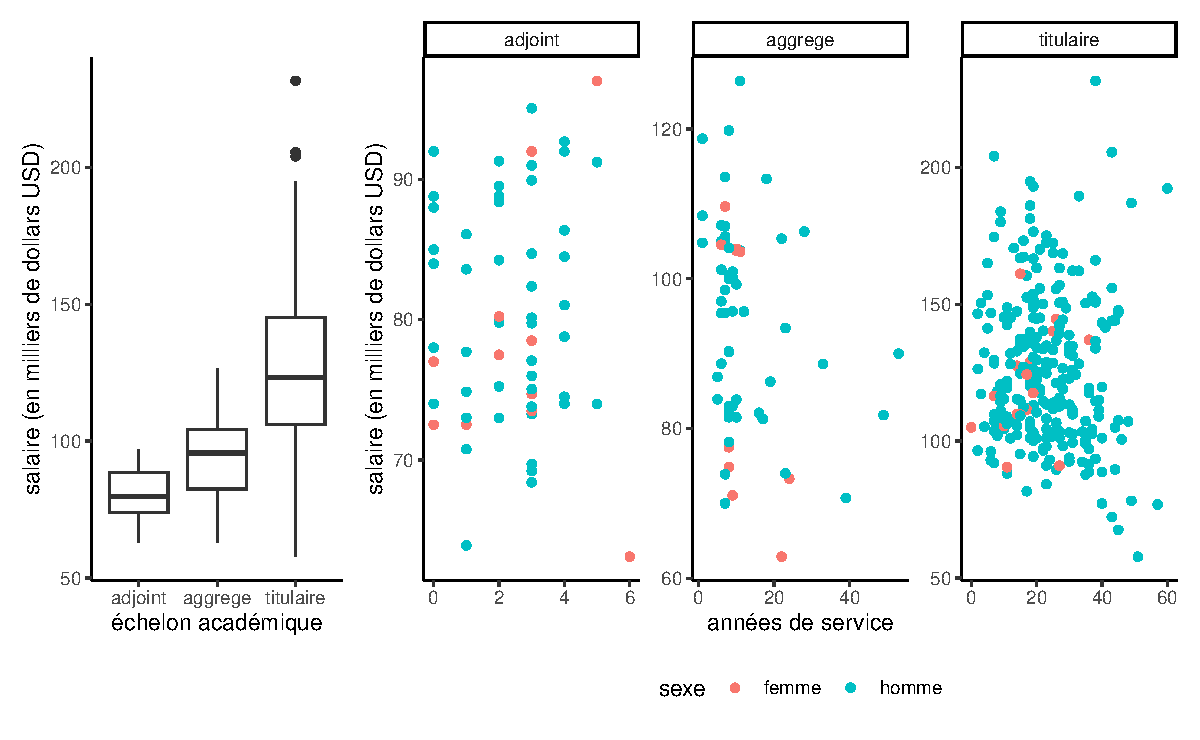
\includegraphics[width=0.85\textwidth,height=\textheight]{regression-lineaire_files/figure-pdf/fig-edacollege-1.pdf}

}

\caption{\label{fig-edacollege}Analyse exploratoire des données
\texttt{college}: répartition des salaires en fonction de l'échelon et
du nombre d'années de service}

\end{figure}%

Ainsi, le salaire augmente avec les années, mais la variabilité croît
également. Les professeurs adjoints qui ne sont pas promus sont
généralement mis à la porte, aussi il y a moins d'occasions pour que les
salaires varient sur cette échelle. Il y a peu de femmes dans
l'échantillon: moins d'information signifie moins de puissance pour
détecter de petites différences de salaire. Si on fait un tableau de
contingence de l'échelon et du sexe, on peut calculer la proportion
relative homme/femme dans chaque échelon: 16\% des profs adjoints, 16\%
pour les aggrégés, mais seulement 7\% des titulaires alors que ces
derniers sont mieux payés en moyenne.

\begin{longtable}[]{@{}lrrr@{}}
\caption{Tableau de contingence donnant le nombre de professeurs du
collège par sexe et par échelon académique.}\tabularnewline
\toprule\noalign{}
& adjoint & aggrege & titulaire \\
\midrule\noalign{}
\endfirsthead
\toprule\noalign{}
& adjoint & aggrege & titulaire \\
\midrule\noalign{}
\endhead
\bottomrule\noalign{}
\endlastfoot
femme & 11 & 10 & 18 \\
homme & 56 & 54 & 248 \\
\end{longtable}

Plusieurs des variables explicatives potentielles des données
\texttt{college} sont cat/gorielles (\texttt{echelon}, \texttt{sexe},
\texttt{discipline}), les deux dernières étant binaires. Les variables
numériques \texttt{annees} et \texttt{service} sont fortement corrélées,
avec une corrélation linéaire de 0.91.

\end{example}

\begin{example}[Analyse exploratoire et données
manquantes]\protect\hypertarget{exm-donnees-manquantes-moon}{}\label{exm-donnees-manquantes-moon}

Il convient de vérifier pour les données de Moon et VanEpps
(\citeproc{ref-Moon.VanEpps:2023}{2023}) que la description de la
collecte coïncide avec la structure. Puisque les personnes qui n'ont pas
donné ne remplissent pas le champ pour le montant, ce dernier indique
une valeur manquante. Tous les montants des dons sont entre 0.25\$ et
25\$.

\begin{Shaded}
\begin{Highlighting}[]
\FunctionTok{data}\NormalTok{(MV23\_S1, }\AttributeTok{package =} \StringTok{"hecedsm"}\NormalTok{)}
\FunctionTok{str}\NormalTok{(MV23\_S1)}
\CommentTok{\#\textgreater{} tibble [869 x 4] (S3: tbl\_df/tbl/data.frame)}
\CommentTok{\#\textgreater{}  $ before   : int [1:869] 0 1 0 1 1 1 1 0 1 0 ...}
\CommentTok{\#\textgreater{}  $ donate   : int [1:869] 0 0 0 1 1 0 1 0 0 1 ...}
\CommentTok{\#\textgreater{}  $ condition: Factor w/ 2 levels "open{-}ended","quantity": 1 1 1 1 2 2 2 1 1 1 ...}
\CommentTok{\#\textgreater{}  $ amount   : num [1:869] NA NA NA 10 5 NA 20 NA NA 25 ...}
\FunctionTok{summary}\NormalTok{(MV23\_S1)}
\CommentTok{\#\textgreater{}      before          donate          condition       amount    }
\CommentTok{\#\textgreater{}  Min.   :0.000   Min.   :0.00   open{-}ended:407   Min.   : 0.2  }
\CommentTok{\#\textgreater{}  1st Qu.:0.000   1st Qu.:0.00   quantity  :462   1st Qu.: 5.0  }
\CommentTok{\#\textgreater{}  Median :1.000   Median :1.00                    Median :10.0  }
\CommentTok{\#\textgreater{}  Mean   :0.596   Mean   :0.73                    Mean   :10.7  }
\CommentTok{\#\textgreater{}  3rd Qu.:1.000   3rd Qu.:1.00                    3rd Qu.:15.0  }
\CommentTok{\#\textgreater{}  Max.   :1.000   Max.   :1.00                    Max.   :25.0  }
\CommentTok{\#\textgreater{}  NA\textquotesingle{}s   :1                                       NA\textquotesingle{}s   :235}
\end{Highlighting}
\end{Shaded}

Si nous incluons \texttt{amount} comme variable réponse dans un modèle
de régression, les 235 observations manquantes seront supprimées par
défaut. Cela ne pose pas de problème si nous voulons comparer le montant
moyen des personnes qui ont fait un don, mais dans le cas contraire,
nous devons transformer les \texttt{NA} en zéros. La variable
\texttt{donate} ne doit pas être incluse comme variable explicative dans
le modèle, car elle permet de prédire exactement les personnes qui n'ont
pas donné.

\end{example}

\subsection{Spécification du modèle pour la
moyenne}\label{spuxe9cification-du-moduxe8le-pour-la-moyenne}

La première étape d'une analyse consiste à décider quelles variables
explicatives doivent être ajoutées à l'équation de la moyenne, et sous
quelle forme. Les modèles ne sont que des approximations de la réalité;
la section 2.1 de Venables (\citeproc{ref-Venables:2000}{2000}) affirme
que, si nous pensons que la véritable fonction moyenne reliant les
variables explicatives \(\boldsymbol{X}\) et la réponse \(Y\) est de la
forme \(\mathsf{E}(Y \mid \boldsymbol{X}) = f(\boldsymbol{X})\) pour
\(f\) suffisamment lisse, alors le modèle linéaire est une approximation
du premier ordre. À des fins d'interprétation, il est logique de centrer
sur la moyenne toute variable explicative continue, car cela facilite
l'interprétation.

Dans un cadre expérimental, où la condition expérimentale est attribué
de manière aléatoire, nous pouvons directement comparer les différents
traitements et tirer des conclusions causales (puisque toutes les autres
choses sont égales en moyenne constantes, toute différence détectable
est due en moyenne à notre manipulation). Bien que nous nous abstenions
généralement d'inclure d'autres variables explicatives afin de préserver
la simplicité du modèle, il peut néanmoins être utile de prendre en
compte certaines variables concomitantes qui expliquent une partie de la
variabilité afin de filtrer le bruit de fond et d'augmenter la puissance
de l'étude. Par exemple, pour les données de Baumann, Seifert-Kessell,
et Jones (\citeproc{ref-Baumann:1992}{1992}), l'objectif est de comparer
les scores moyens en fonction de la méthode d'enseignement, nous
inclurions \texttt{group}. Dans cet exemple, il serait également logique
d'inclure le résultat \texttt{pretest1} en tant qu'élément explicatif
pour \texttt{posttest1}. De cette façon, nous modéliserons la différence
moyenne d'amélioration entre le pré-test et le post-test plutôt que le
résultat final.

Dans un contexte observationnel, les participants dans différents
groupes ont des caractéristiques différentes et nous devons donc tenir
compte de ces différences. Les modèles linéaires utilisés en économie et
en finance contiennent souvent des variables de contrôle au modèle pour
tenir compte des différences potentielles dues aux variables
sociodémographiques (âge, revenu, etc.) qui seraient corrélées à
l'appartenance aux groupes. Tout test de coefficients ne prendrait en
compte que la corrélation entre le résultat \(Y\) et le facteur
explicatif postulé d'intérêt.

\section{Interprétation des
coefficients}\label{interpruxe9tation-des-coefficients}

La spécification de la moyenne est \begin{align*}
\mathsf{E}(Y_i \mid \boldsymbol{X}_i = \boldsymbol{x}_i) = \beta_0 + \beta_1 x_{i1} + \cdots + \beta_p x_{ip}.
\end{align*} L'\textbf{ordonnée à l'origine} \(\beta_0\) est la
\textbf{valeur moyenne de \(Y\)} lorsque toutes les variables
explicatives du modèles sont nulles, soit
\(\boldsymbol{x}_i=\boldsymbol{0}_p\). \begin{align*}
\beta_0 &= \mathsf{E}(Y \mid X_1=0,X_2=0,\ldots,X_p=0) \\
&= \beta_0 + \beta_1 \times 0 + \beta_2 \times 0 + \cdots + \beta_p \times 0
\end{align*} Bien sur, il se peut que cette interprétation n'ait aucun
sens dans le contexte étudié. Centrer les variables explicatives
numériques (pour que leurs moyennes soit zéro) permet de rendre
l'ordonnée à l'origine plus interprétable.

En régression linéaire, le paramètre \(\beta_j\) mesure l'effet de la
variable \(X_j\) sur la variable \(Y\) une fois que l'on tient compte
des effets des autres variables explicatives. Pour chaque augmentation
d'une unité de \(X_j\), la réponse \(Y\) augmente en moyenne de
\(\beta_j\) lorsque les autres variables demeurent inchangées,
\begin{align*}
\beta_j &= \mathsf{E}(Y \mid X_j= x_j+1, \boldsymbol{X}_{-j} = \boldsymbol{x}_{-j})  - \mathsf{E}(Y \mid \boldsymbol{X} = \boldsymbol{x}) \\
&= \sum_{\substack{k=1\\k \neq j}}^p \beta_kx_k + \beta_j(x_j+1) - \sum_{k=1}^p \beta_k x_k
\end{align*}

\begin{definition}[Effet
marginal]\protect\hypertarget{def-effet-marginal}{}\label{def-effet-marginal}

On définit l'effet marginal comme la dérivée première de la moyenne
conditionnelle par rapport à \(X_j\), soit
\[\text{effet marginal de }X_j =  \frac{\partial \mathsf{E}(Y \mid \boldsymbol{X})}{ \partial X_j}.\]
Le coefficient \(\beta_j\) est aussi l'\emph{effet marginal} de la
variable \(X_j\).

\end{definition}

Les variables indicatrices, qui prennent typiquement des valeurs de
\(-1\), \(0\) et \(1\), servent à indiquer l'appartenance aux
différentes modalités d'une variable catégorielle. Par exemple, pour une
variable indicatrice binaire, nous pouvons créer une colonne dont les
entrées sont \(1\) pour le groupe de traitement et \(0\) pour le groupe
de contrôle.

\begin{example}[Modèle linéaire avec une seule variable
binaire]\protect\hypertarget{exm-moon}{}\label{exm-moon}

Considérons par exemple un modèle linéaire pour les données de Moon et
VanEpps (\citeproc{ref-Moon.VanEpps:2023}{2023}) qui inclut le montant
(\texttt{amount}) (en dollars, de 0 pour les personnes qui n'ont pas
fait de don, jusqu'à 25 dollars).

L'équation du modèle linéaire simple qui inclut la variable binaire
\texttt{condition} est \begin{align*}
\mathsf{E}(\texttt{amount} \mid \texttt{condition})&= \beta_0 + \beta_1 \mathbf{1}_{\texttt{condition}=\texttt{quantity}}.
\\&= \begin{cases}
\beta_0, & \texttt{condition}=0, \\
\beta_0 + \beta_1 & \texttt{condition}=1.
\end{cases}
\end{align*} Soit \(\mu_0\) l'espérance du montant pour le groupe
contrôle (\texttt{open-ended}) et \(\mu_1\) celui des participants du
groupe de traitement (\texttt{quantity}). Un modèle linéaire qui ne
contient qu'une variable binaire \(X\) comme régresseur revient à
spécifier une moyenne différente pour chacun des deux groupes.
L'ordonnée à l'origine \(\beta_0\) est la moyenne du groupe contrôle. La
moyenne du groupe traitement (\texttt{quantity}) est
\(\beta_0 + \beta_1 = \mu_1\) et donc \(\beta_1=\mu_1-\mu_0\) est la
différence du montant moyen de dons entre le groupe \texttt{open-ended}
et le groupe \texttt{quantity}. Cette paramétrisation est commode si on
veut tester s'il y a une différence moyenne entre les deux groupes,
puisque cette hypothèse nulle correspond à \(\mathscr{H}_0: \beta_1=0\).

\begin{figure}[ht!]

\centering{

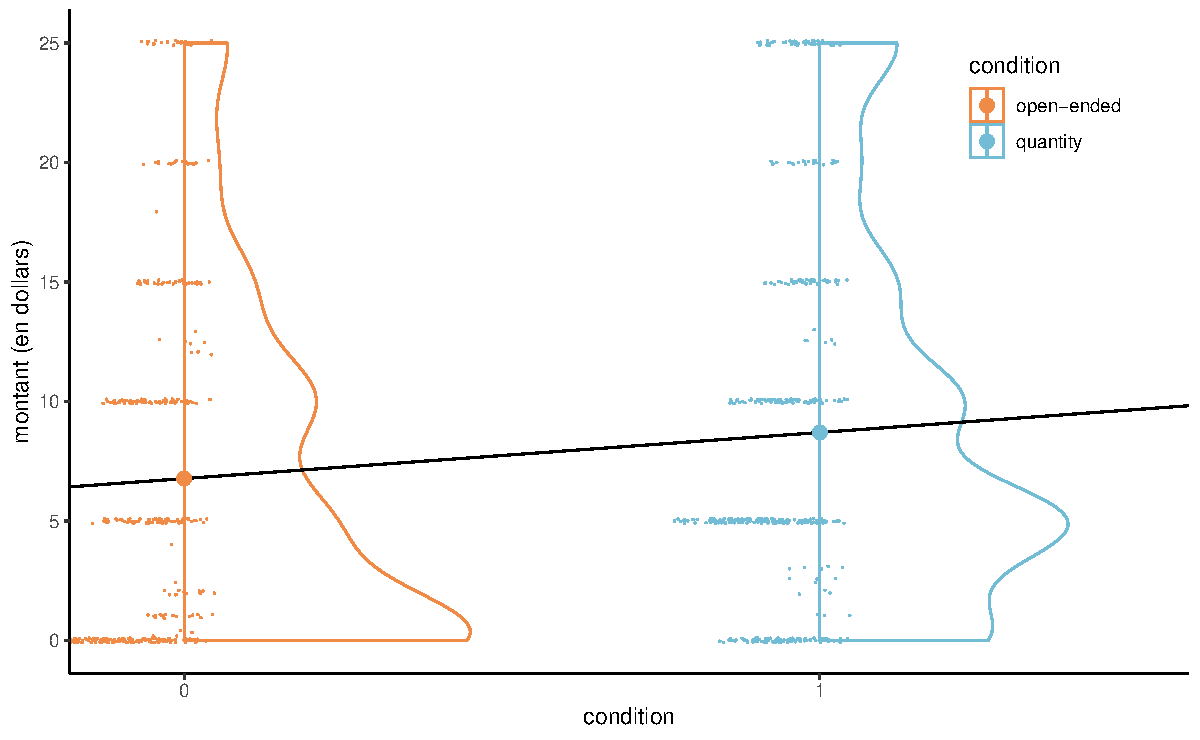
\includegraphics[width=0.85\textwidth,height=\textheight]{regression-lineaire_files/figure-pdf/fig-donation-moon-1.pdf}

}

\caption{\label{fig-donation-moon}Modèle linéaire simple pour les
données \texttt{MV23\_S1} avec \texttt{condition} comme variable
explicative binaire, avec nuage de points décalés et un diagramme en
demi-violin. Les cercles indiquent les moyennes de l'échantillon.}

\end{figure}%

Même si le modèle linéaire définit une droite, cette dernière ne peut
être évaluée qu'à \(0\) ou \(1\); la Figure~\ref{fig-donation-moon}
montre cette droite avec en plus un nuage de points des montants,
décalés horizontalement, et de la densité pour chaque condition. Le
point coloré indique la moyenne empirique, qui correspond aux
estimations.

Même s'il est clair que les données sont fortement discrétisées avec
beaucoup de doublons et de zéros, l'échantillon a une taille de 869
observations, donc les conclusions quant aux moyennes de groupe seront
fiables.

\end{example}

Considérons des variables catégorielles avec \(K > 2\) niveaux, qui dans
\textbf{R} sont de la classe \texttt{factor}. La paramétrisation par
défaut des facteurs se fait en termes de contraste de traitement: le
niveau de référence du facteur (par défaut, la première valeur dans
l'ordre alphanumérique) sera traité comme la catégorie de référence et
assimilé à l'ordonnée à l'origine. Le logiciel créera alors un ensemble
de \(K-1\) variables indicatrices pour un facteur à \(K\) niveaux,
chacune d'entre elles ayant un pour la catégorie représentée et zéro
dans le cas contraire.

\begin{example}[Codage binaire pour les variables
catégorielles]\protect\hypertarget{exm-baumann-dummies}{}\label{exm-baumann-dummies}

Considérons l'étude de Baumann, Seifert-Kessell, et Jones
(\citeproc{ref-Baumann:1992}{1992}) et la seule variable \texttt{group}.
Les données sont classées par groupe : les 22 premières observations
concernent le groupe \texttt{DR}, les 22 suivantes le groupe
\texttt{DRTA} et les 22 dernières le groupe \texttt{TA}. Si nous
ajustons un modèle avec \texttt{groupe} comme variable catégorielle

\begin{Shaded}
\begin{Highlighting}[]
\FunctionTok{data}\NormalTok{(BSJ92, }\AttributeTok{package =} \StringTok{"hecedsm"}\NormalTok{)}
\FunctionTok{class}\NormalTok{(BSJ92}\SpecialCharTok{$}\NormalTok{group) }\CommentTok{\# Vérifier que group est un facteur}
\CommentTok{\#\textgreater{} [1] "factor"}
\FunctionTok{levels}\NormalTok{(BSJ92}\SpecialCharTok{$}\NormalTok{group) }\CommentTok{\# première valeur est la catégorie de référence}
\CommentTok{\#\textgreater{} [1] "DR"   "DRTA" "TA"}
\CommentTok{\# Imprimer trois lignes de la matrice du modèle}
\CommentTok{\# (trois enfants de groupes différents)}
\FunctionTok{model.matrix}\NormalTok{(}\SpecialCharTok{\textasciitilde{}}\NormalTok{ group, }\AttributeTok{data =}\NormalTok{ BSJ92)[}\FunctionTok{c}\NormalTok{(}\DecValTok{1}\NormalTok{,}\DecValTok{23}\NormalTok{,}\DecValTok{47}\NormalTok{),]}
\CommentTok{\#\textgreater{}    (Intercept) groupDRTA groupTA}
\CommentTok{\#\textgreater{} 1            1         0       0}
\CommentTok{\#\textgreater{} 23           1         1       0}
\CommentTok{\#\textgreater{} 47           1         0       1}
\CommentTok{\# Comparer avec les niveaux des facteurs}
\NormalTok{BSJ92}\SpecialCharTok{$}\NormalTok{group[}\FunctionTok{c}\NormalTok{(}\DecValTok{1}\NormalTok{,}\DecValTok{23}\NormalTok{,}\DecValTok{47}\NormalTok{)]}
\CommentTok{\#\textgreater{} [1] DR   DRTA TA  }
\CommentTok{\#\textgreater{} Levels: DR DRTA TA}
\end{Highlighting}
\end{Shaded}

Si nous ajustons un modèle avec \texttt{groupe} comme variable
catégorielle, la spécification de la moyenne du modèle est
\[\mathsf{E}(Y \mid \texttt{group})= \beta_0 + \beta_1\mathbf{1}_{\texttt{group}=\texttt{DRTA}} + \beta_2\mathbf{1}_{\texttt{group}=\texttt{TA}}.\]
Puisque la variable \texttt{group} est catégorielle avec \(K=3\)
niveaux, il nous faut mettre \(K-1 = 2\) variables indicatrices.

Avec la paramétrisation en termes de \textbf{traitements} (option par
défaut), on obtient

\begin{itemize}
\tightlist
\item
  \(\mathbf{1}_{\texttt{group}=\texttt{DRTA}}=1\) si \texttt{group=DRTA}
  et zéro sinon,
\item
  \(\mathbf{1}_{\texttt{group}=\texttt{TA}}=1\) si \texttt{group=TA} et
  zéro sinon.
\end{itemize}

Étant donné que le modèle comprend une ordonnée à l'origine et que le
modèle décrit en fin de compte trois moyennes de groupe, nous n'avons
besoin que de deux variables supplémentaires. Avec la paramétrisation en
termes de \textbf{traitements}, la moyenne du groupe de référence est
l'ordonnée à l'origine. Si \texttt{group}=\texttt{DR} (référence), les
deux variables indicatrices binaires \texttt{groupDRTA} et
\texttt{groupTA} sont nulles. La moyenne de chaque groupe est

\begin{itemize}
\tightlist
\item
  \(\mu_{\texttt{DR}} = \beta_0\),
\item
  \(\mu_{\texttt{DRTA}}=\beta_0 + \beta_1\) et
\item
  \(\mu_{\texttt{TA}} = \beta_0 + \beta_2\).
\end{itemize}

Ainsi, \(\beta_1\) est la différence de moyenne entre les groupes
\texttt{DRTA} et\texttt{DR}, et de la même façon
\(\beta_2=\mu_{\texttt{TA}}- \mu_{\texttt{DR}}\).

\end{example}

\begin{refremark}[Contrainte de somme nulle]
La paramétrisation discutée ci-dessus, qui est la valeur par défaut de
la fonction \texttt{lm}, n'est pas la seule disponible. Plutôt que de
comparer la moyenne de chaque groupe avec celle d'une catégorie de
référence, la paramétrisation par défaut pour les modèles d'analyse de
la variance est en termes de contraintes de somme nulle pour les
coefficients, où l'ordonnée à l'origine est la moyenne équi-pondérée de
chaque groupe, et les paramètres \(\beta_1, \ldots, \beta_{K-1}\) sont
des différences par rapport à cette moyenne.

\begin{Shaded}
\begin{Highlighting}[]
\FunctionTok{model.matrix}\NormalTok{(}
    \SpecialCharTok{\textasciitilde{}}\NormalTok{ group,}
    \AttributeTok{data =}\NormalTok{ BSJ92,}
    \AttributeTok{contrasts.arg =} \FunctionTok{list}\NormalTok{(}\AttributeTok{group =} \StringTok{"contr.sum"}\NormalTok{))}
\end{Highlighting}
\end{Shaded}

\begin{longtable}[]{@{}lrrr@{}}

\caption{\label{tbl-sum2zero}Paramétrisation des variables indicatrices
pour la contrainte de somme nulle pour une variable catégorielle.}

\tabularnewline

\toprule\noalign{}
& (Intercept) & group1 & group2 \\
\midrule\noalign{}
\endhead
\bottomrule\noalign{}
\endlastfoot
DR & 1 & 1 & 0 \\
DRTA & 1 & 0 & 1 \\
TA & 1 & -1 & -1 \\

\end{longtable}

Dans la contrainte de somme nulle, nous obtenons à nouveau deux
variables indicatrices, \texttt{group1} et \texttt{group2}, ainsi que
l'ordonnée à l'origine. La valeur de \texttt{group1} est \(1\) si
\texttt{group=DR}, \(0\) si \texttt{group=DRTA} et \(-1\) si
\texttt{group=TA}. ous trouvons
\(\mu_{\texttt{DR}} = \beta_0 + \beta_1\),
\(\mu_{\texttt{DRTA}}=\beta_0 + \beta_2\) et
\(\mu_{\texttt{TA}} = \beta_0 - \beta_1 - \beta_2\). Quelques
manipulations algébriques révèlent que
\(\beta_0 = (\mu_{\texttt{DR}} +\mu_{\texttt{DRTA}}+\mu_{\texttt{TA}})/3\),
l'espérance équipondérée des différents niveaux. De manière générale,
l'ordonnée à l'origine moins la somme de tous les autres coefficients
liés aux facteurs.

En supprimant l'ordonnée à l'origine, on pourrait inclure trois
variables indicatrices pour chaque niveau d'un facteur et chaque
paramètre correspondrait alors à la moyenne. Ce n'est pas recommandé
dans \textbf{R} car le logiciel traite différemment les modèles sans
ordonnée à l'origine et certains résultats seront absurdes (par exemple,
le coefficient de détermination sera erroné).

\label{rem-sumtozero}

\end{refremark}

\begin{example}[Interprétation des
coefficients]\protect\hypertarget{exm-college-coeff}{}\label{exm-college-coeff}

On considère un modèle de régression pour les données \texttt{college}
qui inclut le sexe, l'échelon académique, le nombre d'années de service
et le domaine d'expertise (appliquée ou théorique).

Le modèle linéaire postulé s'écrit

\begin{align*}
\texttt{salaire} &= \beta_0 + \beta_1 \mathbf{1}_{\texttt{sexe}=\texttt{femme}} +\beta_2 \mathbf{1}_{\texttt{domaine}=\texttt{theorique}} \\&\quad +\beta_3 \mathbf{1}_{\texttt{echelon}=\texttt{aggrege}}
+\beta_4 \mathbf{1}_{\texttt{echelon}=\texttt{titulaire}} \\&\quad+\beta_5 \texttt{service} + \varepsilon.
\end{align*}

\begin{longtable}[]{@{}
  >{\raggedleft\arraybackslash}p{(\columnwidth - 10\tabcolsep) * \real{0.1667}}
  >{\raggedleft\arraybackslash}p{(\columnwidth - 10\tabcolsep) * \real{0.1667}}
  >{\raggedleft\arraybackslash}p{(\columnwidth - 10\tabcolsep) * \real{0.1667}}
  >{\raggedleft\arraybackslash}p{(\columnwidth - 10\tabcolsep) * \real{0.1667}}
  >{\raggedleft\arraybackslash}p{(\columnwidth - 10\tabcolsep) * \real{0.1667}}
  >{\raggedleft\arraybackslash}p{(\columnwidth - 10\tabcolsep) * \real{0.1667}}@{}}

\caption{\label{tbl-collegecoefs}Estimations des coefficients du modèle
linéaire pour les données \(\texttt{college}\) (en dollars USD, arrondis
à l'unité).}

\tabularnewline

\toprule\noalign{}
\begin{minipage}[b]{\linewidth}\raggedleft
\(\widehat{\beta}_0\)
\end{minipage} & \begin{minipage}[b]{\linewidth}\raggedleft
\(\widehat{\beta}_1\)
\end{minipage} & \begin{minipage}[b]{\linewidth}\raggedleft
\(\widehat{\beta}_2\)
\end{minipage} & \begin{minipage}[b]{\linewidth}\raggedleft
\(\widehat{\beta}_3\)
\end{minipage} & \begin{minipage}[b]{\linewidth}\raggedleft
\(\widehat{\beta}_4\)
\end{minipage} & \begin{minipage}[b]{\linewidth}\raggedleft
\(\widehat{\beta}_5\)
\end{minipage} \\
\midrule\noalign{}
\endhead
\bottomrule\noalign{}
\endlastfoot
86596 & -4771 & -13473 & 14560 & 49160 & -89 \\

\end{longtable}

L'interprétation des coefficients est la suivante:

\begin{itemize}
\tightlist
\item
  L'ordonnée à l'origine \(\beta_0\) correspond au salaire moyen d'un
  professeur adjoint (un homme) qui vient de compléter ses études et qui
  travaille dans un domaine appliqué: on estime ce salaire à
  \(\widehat{\beta}_0=86596\) dollars.
\item
  toutes choses étant égales par ailleurs (même domaine, échelon et
  années depuis le dernier diplôme), l'écart de salaire entre un homme
  et un femme est estimé à \(\widehat{\beta}_1=-4771\) dollars.
\item
  \emph{ceteris paribus}, un(e) professeur(e) qui oeuvre dans un domaine
  théorique gagne \(\beta_2\) dollars de plus qu'une personne du même
  sexe dans un domaine appliqué; on estime cette différence à \(-13473\)
  dollars.
\item
  \emph{ceteris paribus}, la différence moyenne de salaire entre
  professeurs adjoints et aggrégés est estimée à
  \(\widehat{\beta}_3=14560\) dollars.
\item
  \emph{ceteris paribus}, la différence moyenne de salaire entre
  professeurs adjoints et titulaires est de \(\widehat{\beta}_4=49160\)
  dollars.
\item
  au sein d'un même échelon, chaque année supplémentaire de service mène
  à une augmentation de salaire annuelle moyenne de
  \(\widehat{\beta}_5=-89\) dollars.
\end{itemize}

\end{example}

\begin{refremark}[Polynômes]
Il n'est pas toujours possible de fixer la valeur des autres colonnes de
\(\mathbf{X}\) si plusieurs colonnes contiennent des transformations ou
des fonctions d'une même variable explicative. Par exemple, on pourrait
par exemple considérer un polynôme d'ordre \(k\) (ordinairement, on va
prendre \(k\leq 3\)), \begin{align*}
\mathsf{E}(Y \mid X=x)=\beta_0+ \beta_1 x+ \beta_2 x^2 + \cdots +\beta_k x^k.
\end{align*} Si l'on inclut un terme d'ordre \(k\), \(x^k\), il faut
\textbf{toujours} inclure les termes d'ordre inférieur
\(1, x, \ldots, x^{k-1}\) pour l'interprétabilité du modèle résultant
(autrement, cela revient à choisir un polynôme en imposant que certains
coefficients soient zéros). L'interprétation des effets des covariables
nonlinéaires (même polynomiaux) est complexe parce qu'on ne peut pas «
fixer la valeur des autres variables »: l'effet d'une augmentation d'une
unité de \(x\) \emph{dépend de la valeur de cette dernière}. L'effet
marginal de \(x\) est \(\beta_1 + \sum_{j=1}^{k-1}j \beta_{j+1}x^j\).

L'utilisation de polynôme, plus flexibles, n'est généralement pas
recommendée car ces derniers se généralisent mal hors de l'étendue
observée des données. L'utilisation de splines avec une pénalité sur les
coefficients, avec des modèles additifs, offre plus de flexibilité.

\label{rem-polynomes}

\end{refremark}

\begin{example}[Modèle quadratique pour les données
automobile]\protect\hypertarget{exm-quadmod}{}\label{exm-quadmod}

Considérons un modèle de régression linéaire pour l'autonomie d'essence
en fonction de la puissance du moteur pour différentes voitures dont les
caractéristiques sont données dans le jeu de données
\texttt{automobiles}. Le modèle postulé incluant un terme quadratique
est \begin{align*}
\texttt{autonomie}_i = \beta_0 + \beta_1 \texttt{puissance}_i + \beta_2 \texttt{puissance}_i^2 + \varepsilon_i
\end{align*} Afin de comparer l'ajustement du modèle quadratique, on
peut inclure également la droite ajustée du modèle de régression simple
qui n'inclut que puissance.

\begin{figure}[ht!]

\centering{

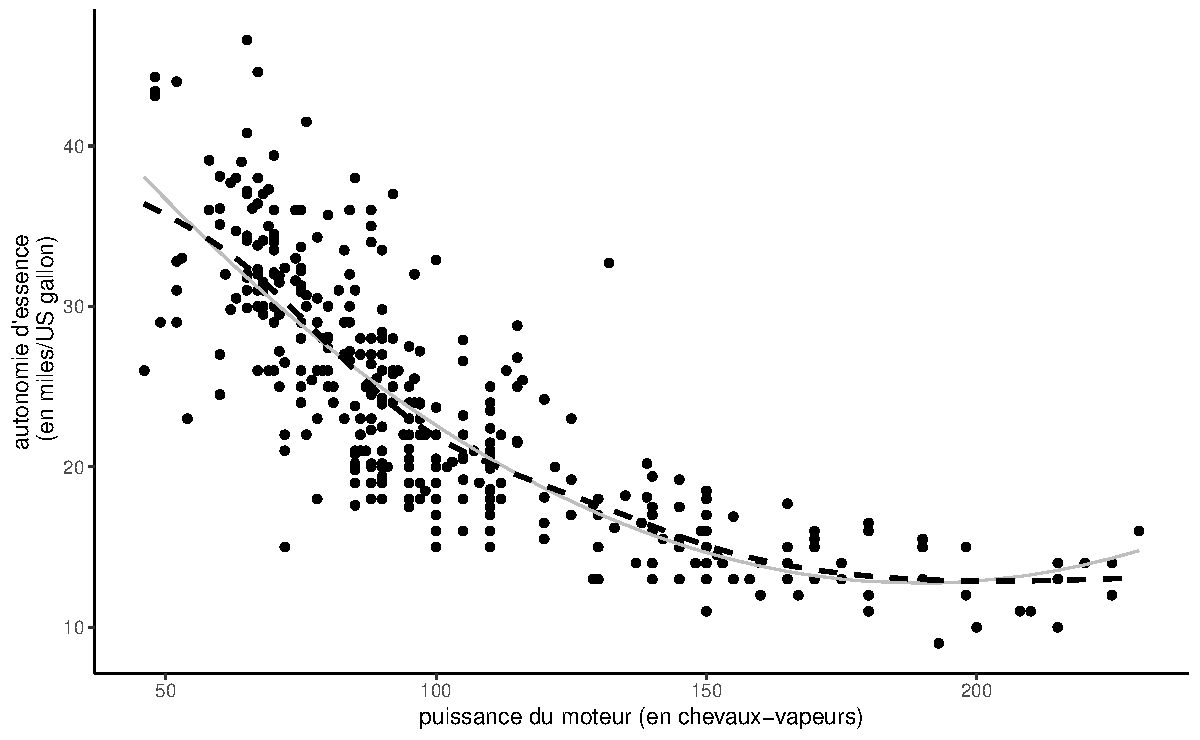
\includegraphics[width=0.85\textwidth,height=\textheight]{regression-lineaire_files/figure-pdf/fig-autoquad2d-1.pdf}

}

\caption{\label{fig-autoquad2d}Modèle de régression avec terme
quadratique pour la puissance (gris), versus spline cubique pénalisée
(ligne traitillée).}

\end{figure}%

À vue d'oeil, l'ajustement quadratique est bon: nous verrons plus tard à
l'aide de test si une simple droite aurait été suffisante. On voit aussi
dans la Figure~\ref{fig-autoquad2d} que l'autonomie d'essence décroît
rapidement quand la puissance croît entre \(0\) et \(189.35\), mais
semble remonter légèrement par la suite pour les voitures qui un moteur
de plus de 200 chevaux-vapeurs, ce que le modèle quadratique capture.
Prenez garde en revanche à l'extrapolation là où vous n'avez pas de
données (comme l'illustre remarquablement bien
\href{https://web.archive.org/web/20210315050023/https://livefreeordichotomize.com/2020/05/05/model-detective/}{le
modèle cubique de Hassett pour le nombre de cas quotidiens de
coronavirus}).

La représentation graphique du modèle polynomial de degré 2 présenté
dans la Figure~\ref{fig-autoquad2d} peut sembler contre-intuitive, mais
c'est une projection en 2D d'un plan 3D de coordonnées
\(\beta_0 + \beta_1x-y +\beta_2z =0\), où \(x=\texttt{puissance}\),
\(z=\texttt{puissance}^2\) et \(y=\texttt{autonomie}\). La physique et
le bon-sens imposent la contrainte \(z = x^2\), et donc les valeurs
ajustées vivent sur une courbe dans un sous-espace du plan ajusté,
représenté en gris dans la Figure~\ref{fig-hyperplan}.

\begin{figure}[ht!]

\centering{

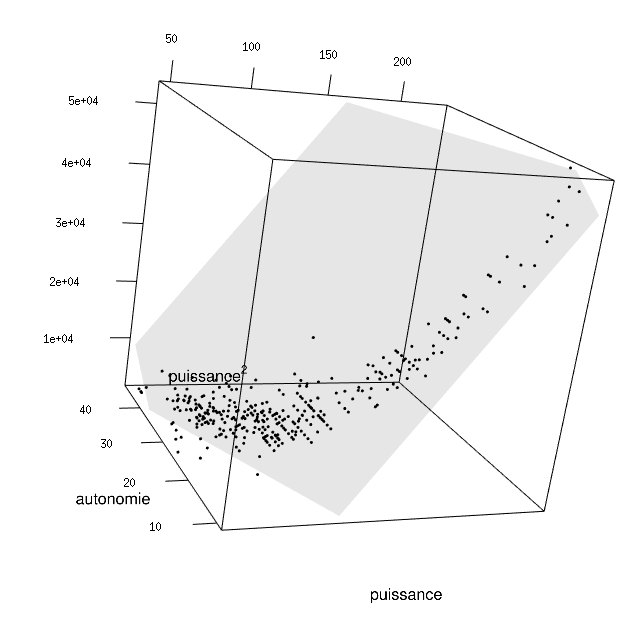
\includegraphics[width=0.85\textwidth,height=\textheight]{images/hyperplan_auto.png}

}

\caption{\label{fig-hyperplan}Représentation graphique 3D du modèle de
régression linéaire pour les données \(\texttt{automobile}\).}

\end{figure}%

\end{example}

\section{Estimation des paramètres}\label{estimation-des-paramuxe8tres}

Considérons un échantillon de \(n\) observations. On n'observe ni les
aléas \(\boldsymbol{\varepsilon}\), ni les paramètres
\(\boldsymbol{\beta}\): il est donc impossible de recouvrer les (vrais)
coefficients du modèle. Effectivement, le système d'équation spécifié
par le modèle linéaire inclut \(n+p+1\) inconnues, mais uniquement \(n\)
observations. Si on se concentre sur les \(p+1\) paramètres de moyenne
et sur la variance \(\sigma^2\), nous pourrons estimer les paramètres
généralement si \(n> p+2\), mais cela dépend de la spécification. Une
infinité de plans pourraient passer dans le nuage de points; il faut
donc choisir la meilleure droite (selon un critère donné). La section
aborde le choix de ce critère et l'estimation des paramètres de la
moyenne.

\subsection{Moindres carrés
ordinaires}\label{moindres-carruxe9s-ordinaires-1}

Soit une matrice de modèle \(\mathbf{X}\) et une formulation pour la
moyenne avec \(\mathsf{E}(Y_i) = \mathbf{x}_i\boldsymbol{\beta}\). Les
estimateurs des moindres carrés ordinaires
\(\widehat{\boldsymbol{\beta}}=(\widehat{\beta}_0, \ldots, \widehat{\beta}_p)\)
sont les paramètres qui minimisent simultanément la distance euclidienne
entre les observations \(y_i\) et les \textbf{valeurs ajustées}
\(\widehat{y}_i=\mathbf{x}_i\widehat{\boldsymbol{\beta}}\).

\begin{figure}[ht!]

\centering{

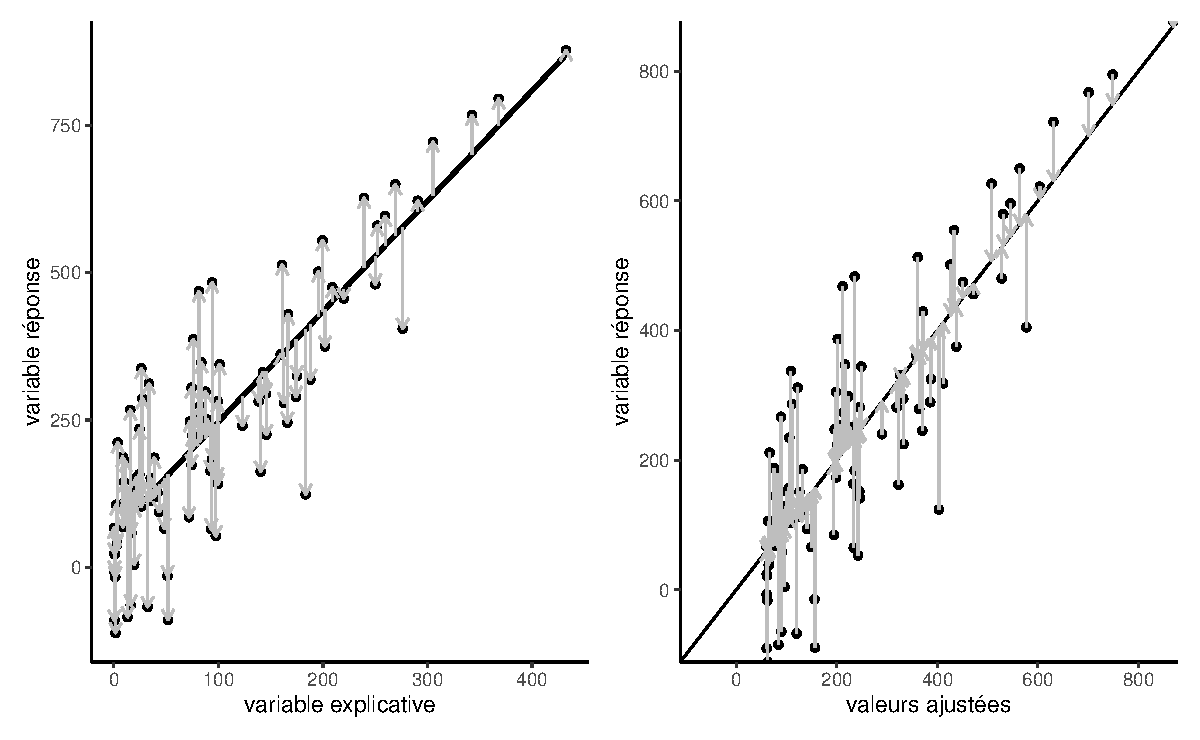
\includegraphics[width=0.85\textwidth,height=\textheight]{regression-lineaire_files/figure-pdf/fig-vertdist-1.pdf}

}

\caption{\label{fig-vertdist}Résidus ordinaires \(e_i\) (vecteurs
verticaux) ajoutés à la droit de régression dans l'espace \((x, y)\)
(gauche) et l'ajustement de la variable réponse \(y_i\) en fonction des
valeurs ajustées \(\widehat{y}_i\).}

\end{figure}%

En d'autres mots, les estimateurs des moindres carrés sont la solution
du problème d'optimization convexe \begin{align*}
\widehat{\boldsymbol{\beta}} &=\min_{\boldsymbol{\beta} \in \mathbb{R}^{p+1}}\sum_{i=1}^n (Y_i-\widehat{Y}_i)^2= \min_{\boldsymbol{\beta}} \|\boldsymbol{Y}-\mathbf{X}\boldsymbol{\beta}\|^2
\end{align*} Ce système d'équation a une solution explicite qui est plus
facilement exprimée en notation matricielle. Soit les matrices et
vecteurs \begin{align*}
\boldsymbol{Y} =
 \begin{pmatrix}
  Y_1 \\
  Y_2 \\
  \vdots \\
  Y_n
 \end{pmatrix} ,
 \;
\mathbf{X} = \begin{pmatrix}
1 & x_{11} & x_{12} & \cdots & x_{1p} \\
1 & x_{21} & x_{22} & \cdots & x_{2p} \\
\vdots & \vdots & \ddots & \vdots \\
1 & x_{n1} & x_{n2} & \cdots & x_{np}
\end{pmatrix} , \;
\boldsymbol{\beta} =
 \begin{pmatrix}
  \beta_1 \\
  \beta_2 \\
  \vdots \\
  \beta_p
 \end{pmatrix}
\end{align*}

\begin{proposition}[Moindres carrés
ordinaires]\protect\hypertarget{prp-ols-mle}{}\label{prp-ols-mle}

L'estimateur des moindres carrés ordinaires résoud le problème
d'optimisation non-contraint \begin{align*}
\widehat{\boldsymbol{\beta}}=\min_{\boldsymbol{\beta} \in \mathbb{R}^{p+1}}(\boldsymbol{y}-\mathbf{X}\boldsymbol{\beta})^\top(\boldsymbol{y}-\mathbf{X}\boldsymbol{\beta}).
\end{align*} On peut calculer la dérivée première par rapport à
\(\boldsymbol{\beta}\), égaler à zéro et isoler le maximum pour obtenir
une formule explicite pour \(\widehat{\boldsymbol{\beta}}\),
\begin{align*}
\mathbf{0}_n&=\frac{\partial}{\partial\boldsymbol{\beta}}(\boldsymbol{y}-\mathbf{X}\boldsymbol{\beta})^\top(\boldsymbol{y}-\mathbf{X}\boldsymbol{\beta})\\
\\&=\frac{\partial (\boldsymbol{y}-\mathbf{X}\boldsymbol{\beta})}{\partial \boldsymbol{\beta}}\frac{\partial (\boldsymbol{y}-\mathbf{X}\boldsymbol{\beta})^\top(\boldsymbol{y}-\mathbf{X}\boldsymbol{\beta})}{\partial (\boldsymbol{y}-\mathbf{X}\boldsymbol{\beta})}\\
 \\&=\mathbf{X}^\top (\boldsymbol{y}-\mathbf{X}\boldsymbol{\beta})
\end{align*} en utilisant la
\href{http://www.stat.rice.edu/~dobelman/notes_papers/math/Matrix.Calculus.AppD.pdf}{règle
de dérivation en chaîne}; on peut ainsi distribuer les termes pour
obtenir l'\emph{équation normale} \begin{align*}
 \mathbf{X}^\top \mathbf{X}\boldsymbol{\beta}&=\mathbf{X}^\top \boldsymbol{y}.
\end{align*} Si \(\mathbf{X}\) est une matrice de rang \(p\), alors la
forme quadratique \(\mathbf{X}^\top \mathbf{X}\) est inversible et
l'unique solution du problème d'optimisation est \begin{align*}
\widehat{\boldsymbol{\beta}} = (\mathbf{X}^{\top} \mathbf{X})^{-1} \mathbf{X}^{\top} \boldsymbol{Y}.
\end{align*} Si le rang de la matrice \(\mathbf{X}\) est dimension
\(n \times (p+1)\) est de rang \(p+1\), l'unique solution du problème
d'optimisation est \begin{equation}\phantomsection\label{eq-ols}{
\widehat{\boldsymbol{\beta}} = (\mathbf{X}^{\top} \mathbf{X})^{-1} \mathbf{X}^{\top} \boldsymbol{Y}.
}\end{equation} Cet estimateur dit des \textbf{moindres carrés
ordinaires} (MCO) est explicite; il n'est donc pas nécessaire de
procéder à l'optimisation à l'aide d'algorithmes numériques.

\end{proposition}

\subsection{Maximum de vraisemblance}\label{maximum-de-vraisemblance}

Nous pourrions également envisager l'estimation du maximum de
vraisemblance. Proposition~\ref{prp-mle-normal-linmod} montre que, en
supposant la normalité des aléas, les estimateurs des moindres carrés de
\(\boldsymbol{\beta}\) coïncident avec ceux du maximum de vraisemblance.

\begin{proposition}[Estimation du maximum de vraisemblance du modèle
linéaire
normal]\protect\hypertarget{prp-mle-normal-linmod}{}\label{prp-mle-normal-linmod}

Le modèle de régression linéaire spécifie que les observations
\(Y_i \sim \mathsf{normale}(\mathbf{x}_i\boldsymbol{\beta}, \sigma^2)\)
sont indépendantes. Le modèle linéaire a \(p+2\) paramètres
(\(\boldsymbol{\beta}\) et \(\sigma^2\)) et la log-vraisemblance est,
abstraction faite des termes constants, \begin{align*}
\ell(\boldsymbol{\beta}, \sigma)&\propto-\frac{n}{2} \ln (\sigma^2) -\frac{1}{2\sigma^2}\left\{(\boldsymbol{y}-\mathbf{X}\boldsymbol{\beta})^\top(\boldsymbol{y}-\mathbf{X}\boldsymbol{\beta})\right\}^2.
\end{align*} Maximiser la log-vraisemblance par rapport à
\(\boldsymbol{\beta}\) revient à minimiser la somme du carré des erreurs
\(\sum_{i=1}^n (y_i - \mathbf{x}_i\boldsymbol{\beta})^2\), quelle que
soit la valeur de \(\sigma\), et on recouvre
\(\widehat{\boldsymbol{\beta}}\). L'estimateur du maximum de
vraisemblance de la variance \(\widehat{\sigma}^2\) est \begin{align*}
\widehat{\sigma}^2=\mathrm{arg max}_{\sigma^2} \ell(\widehat{\boldsymbol{\beta}}, \sigma^2).
\end{align*} La log-vraisemblance profilée de \(\sigma^2\), abstraction
faite des constantes, est \begin{align*}
\ell_{\mathrm{p}}(\sigma^2)
&\propto-\frac{1}{2}\left\{n\ln\sigma^2+\frac{1}{\sigma^2}(\boldsymbol{y}-\mathbf{X}\hat{\boldsymbol{\beta}})^\top(\boldsymbol{y}-\mathbf{X}\hat{\boldsymbol{\beta}})\right\}.
\end{align*} En différenciant chaque terme par rapport à \(\sigma^2\) et
en fixant le gradient à zéro, on obtient \begin{align*}
\frac{\partial \ell_{\mathrm{p}}(\sigma^2)}{\partial \sigma^2} = -\frac{n}{2\sigma^2} + \frac{(\boldsymbol{y}-\mathbf{X}\hat{\boldsymbol{\beta}})^\top(\boldsymbol{y}-\mathbf{X}\hat{\boldsymbol{\beta}})}{2\sigma^4} = 0
\end{align*}

On déduit que l'estimateur du maximum de vraisemblance est la moyenne
des carrés des résidus, \begin{align*}
\widehat{\sigma}^2&=\frac{1}{n}(\boldsymbol{Y}-\mathbf{X}\hat{\boldsymbol{\beta}})^\top(\boldsymbol{Y}-\mathbf{X}\hat{\boldsymbol{\beta}})\\&= \frac{1}{n} \sum_{i=1}^n (y_i - \mathbf{x}_i\widehat{\boldsymbol{\beta}})^2= \frac{\mathsf{SC}_e}{n};
\end{align*} L'estimateur sans biais habituel de \(\sigma^2\) calculé
par le logiciel est \[S^2=\mathsf{SC}_e/(n-p-1),
\] où le dénominateur est la taille de l'échantillon \(n\) moins le
nombre de paramètres de la moyenne \(\boldsymbol{\beta}\), soit \(p+1\).

\end{proposition}

\begin{proposition}[Matrices d'information pour modèles linéaires
normaux.]\protect\hypertarget{prp-info-normal}{}\label{prp-info-normal}

Les entrées de la matrice d'information observée du modèle linéaire
normal sont les suivantes \begin{align*}
-\frac{\partial^2 \ell(\boldsymbol{\beta}, \sigma^2)}{\partial \boldsymbol{\beta}\partial \boldsymbol{\beta}^\top} &= \frac{1}{\sigma^2} \frac{\partial \mathbf{X}^\top(\boldsymbol{y}-\mathbf{X}\boldsymbol{\beta})}{\partial \boldsymbol{\beta}^\top} =  \frac{\mathbf{X}^\top\mathbf{X}}{\sigma^2}\\
-\frac{\partial^2 \ell(\boldsymbol{\beta}, \sigma^2)}{\partial \boldsymbol{\beta}\partial \sigma^2} &=- \frac{\mathbf{X}^\top(\boldsymbol{y}-\mathbf{X}\boldsymbol{\beta})}{\sigma^4}\\
-\frac{\partial^2 \ell(\boldsymbol{\beta}, \sigma^2)}{\partial (\sigma^2)^2} &= -\frac{n}{2\sigma^4} + \frac{(\boldsymbol{y}-\mathbf{X}\boldsymbol{\beta})^\top(\boldsymbol{y}-\mathbf{X}\boldsymbol{\beta})}{\sigma^6}.
\end{align*} Si on évalue l'information observée aux EMV, on obtient
\begin{align*}
j(\widehat{\boldsymbol{\beta}}, \widehat{\sigma^2}) = 
\begin{pmatrix}
\frac{\mathbf{X}^\top\mathbf{X}}{\widehat{\sigma^2}} & \boldsymbol{0}_{p+1} \\  \boldsymbol{0}_{p+1}^\top & \frac{n}{2\widehat{\sigma^4}}
\end{pmatrix}
\end{align*} puisque \(\widehat{\sigma}^2=\mathsf{SC}_e/n\) et que les
résidus sont orthogonaux à la matrice du modèle. Sachant que
\(\mathsf{E}(Y \mid \mathbf{X})=\mathbf{X}\boldsymbol{\beta}\), la
matrice d'information de Fisher est \begin{align*}
i(\boldsymbol{\beta}, \sigma^2) = 
\begin{pmatrix}
\frac{\mathbf{X}^\top\mathbf{X}}{\sigma^2} & \boldsymbol{0}_{p+1} \\  \boldsymbol{0}_{p+1}^\top & \frac{n}{2\sigma^4}
\end{pmatrix}
\end{align*} Puisque la loi asymptotique de l'estimateur est normale,
les EMV de \(\sigma^2\) et \(\boldsymbol{\beta}\) sont asymptotiquement
indépendants car leur corrélation asymptotique est nulle.Pourvu que la
matrice carrée \((p+1)\), \(\mathbf{X}^\top\mathbf{X}\) soit inversible,
la variance asymptotique des estimateurs est
\(\mathsf{Var}(\widehat{\boldsymbol{\beta}})=\sigma^2(\mathbf{X}^\top\mathbf{X})^{-1}\)
et \(\mathsf{Var}(\widehat{\sigma}^2) = 2\sigma^4/n\).

\end{proposition}

\begin{refremark}
Si on suppose que les observations sont normales, alors on peut montrer
que \(\mathsf{SC}_e/\sigma^2 \sim \chi^2_{n-p-1}\) et
\(\widehat{\boldsymbol{\beta}} \sim \mathsf{normale}\{\boldsymbol{\beta}, \sigma^2(\mathbf{X}^\top\mathbf{X})^{-1}\}\)
sont indépendants et leurs lois sont connues. Cela nous permettra de
construire des tests d'hypothèse.

\label{rem-independance}

\end{refremark}

\subsection{Ajustement des modèles linéaires à l'aide d'un
logiciel}\label{ajustement-des-moduxe8les-linuxe9aires-uxe0-laide-dun-logiciel}

Bien que nous puissions construire la matrice du modèle nous-mêmes et
utiliser la formule des moindres carrés de l'Équation~\ref{eq-ols}, les
routines numériques implémentées dans les logiciels sont préférables car
plus stables. La fonction \texttt{lm} dans \textbf{R} ajuste \textbf{les
modèles linéaires}, tout comme \texttt{glm} avec les arguments par
défaut. Les objets de la classe \texttt{lm} ont plusieurs méthodes qui
vous permettent d'extraire des objets spécifiques des objets
\texttt{lm}. Par exemple, les fonctions \texttt{coef}, \texttt{resid},
\texttt{fitted}, \texttt{model.matrix} renvoient les estimations des
coefficients \(\widehat{\boldsymbol{\beta}},\) les résidus ordinaires
\(\boldsymbol{e},\) les valeurs ajustées \(\widehat{\boldsymbol{y}}\) et
la matrice du modèle \(\mathbf{X}\).

\begin{Shaded}
\begin{Highlighting}[]
\FunctionTok{data}\NormalTok{(BSJ92, }\AttributeTok{package =} \StringTok{"hecedsm"}\NormalTok{) }\CommentTok{\# charger les données}
\FunctionTok{str}\NormalTok{(BSJ92) }\CommentTok{\# vérifier que les variables catégorielles sont "factor"}
\CommentTok{\# Ajustement de la régression linéaire}
\NormalTok{linmod }\OtherTok{\textless{}{-}} \FunctionTok{lm}\NormalTok{(posttest1 }\SpecialCharTok{\textasciitilde{}}\NormalTok{ pretest1 }\SpecialCharTok{+}\NormalTok{ group, }
             \AttributeTok{data =}\NormalTok{ BSJ92)}
\NormalTok{est\_beta }\OtherTok{\textless{}{-}} \FunctionTok{coef}\NormalTok{(linmod) }\CommentTok{\# coefficients (betas)}
\NormalTok{vcov\_beta }\OtherTok{\textless{}{-}} \FunctionTok{vcov}\NormalTok{(linmod) }\CommentTok{\# matrice de covariance des betas}
\FunctionTok{summary}\NormalTok{(linmod) }\CommentTok{\# tableau résumé}
\NormalTok{beta\_ic }\OtherTok{\textless{}{-}} \FunctionTok{confint}\NormalTok{(linmod) }\CommentTok{\# IC de Wald pour betas}
\NormalTok{y\_adj }\OtherTok{\textless{}{-}} \FunctionTok{fitted}\NormalTok{(linmod) }\CommentTok{\# valeurs ajustées}
\NormalTok{e }\OtherTok{\textless{}{-}} \FunctionTok{resid}\NormalTok{(linmod) }\CommentTok{\# résidus ordinaires}

\CommentTok{\# Vérifier la formule des moindres carrés ordinaires}
\NormalTok{X }\OtherTok{\textless{}{-}} \FunctionTok{model.matrix}\NormalTok{(linmod) }\CommentTok{\# matrice du modèle}
\NormalTok{y }\OtherTok{\textless{}{-}}\NormalTok{ college}\SpecialCharTok{$}\NormalTok{salary}
\FunctionTok{isTRUE}\NormalTok{(}\FunctionTok{all.equal}\NormalTok{(}
  \FunctionTok{c}\NormalTok{(}\FunctionTok{solve}\NormalTok{(}\FunctionTok{t}\NormalTok{(X) }\SpecialCharTok{\%*\%}\NormalTok{ X) }\SpecialCharTok{\%*\%} \FunctionTok{t}\NormalTok{(X) }\SpecialCharTok{\%*\%}\NormalTok{ y),}
  \FunctionTok{as.numeric}\NormalTok{(}\FunctionTok{coef}\NormalTok{(linmod))}
\NormalTok{))}
\end{Highlighting}
\end{Shaded}

La méthode \texttt{summary} est sans doute la plus utile: elle affiche
les estimations des paramètres de la moyenne ainsi que leurs erreurs
type, les valeurs \(t\) pour le test de Wald de l'hypothèse
\(\mathscr{H}_0 : \beta_i=0\) et les valeurs-\(p\) associées. D'autres
statistiques descriptives, portant sur la taille de l'échantillon, les
degrés de liberté, etc. sont données au bas du tableau. Notez que la
fonction \texttt{lm} utilise l'estimateur sans biais de la variance
\(\sigma^2\).

\section{Prédictions}\label{sec-predictions-lm}

Une fois les estimations des coefficients obtenues, on peut calculer les
valeurs ajustées \(\widehat{\boldsymbol{y}}\) avec
\(\mathbf{X}\widehat{\boldsymbol{\beta}}\), où \(\mathbf{X}\) dénote la
matrice du modèle \(n \times (p+1)\). On peut aussi généraliser cette
approche et obtenir une estimation de la moyenne pour n'importe quel
vecteur lignes de covariables
\(\mathbf{x}^* = (1, x^*_1, \ldots, x^*_p)\), sachant que
\(\mathsf{E}(Y \mid \mathbf{x}^*)=\mathbf{x}^*\boldsymbol{\beta}\), en
remplaçant les coefficients inconnus \(\boldsymbol{\beta}\) par leurs
estimations \(\widehat{\boldsymbol{\beta}}\). Pour le modèle postulé,
c'est le meilleur prédicteur linéaire non-biaisé de la moyenne.

Si l'on veut prédire la valeur d'une nouvelle observation, disons
\(Y^*\), dont le vecteur de variables explicatives \(\mathbf{x}^*\) sont
connues, la prédiction sera donc
\(\widehat{y}^* = \mathbf{x}^*\widehat{\boldsymbol{\beta}}\) parce que
\begin{align*}
\mathsf{E}(\widehat{Y}^* \mid \mathbf{X}, \mathbf{x}^*) = \mathsf{E}(\mathbf{x}^*\widehat{\boldsymbol{\beta}}\mid \mathbf{X}, \mathbf{x}^*) = \mathbf{x}^*\boldsymbol{\beta}.
\end{align*} Cependant, les observations individuelles varient davantage
que les moyennes (qui sont elles-mêmes basées sur plusieurs
observations). Intuitivement, cela est dû à l'incertitude supplémentaire
du terme d'erreur apparaissant dans l'équation du modèle: la variabilité
des prédictions est la somme de l'incertitude due aux estimateurs (basés
sur des données aléatoires) et de la variance intrinsèque des
observations en supposant que la nouvelle observation est indépendante
de celles utilisées pour estimer les coefficients, \begin{align*}
\mathsf{Va}(Y^*-\widehat{Y}^* \mid \mathbf{X}, \mathbf{x}^*) &= \mathsf{Va}(Y^*  - \mathbf{x}^*\widehat{\boldsymbol{\beta}} \mid \mathbf{X}, \mathbf{x}^*)
\\&=\mathsf{Va}(Y^* \mid \mathbf{X}, \mathbf{x}^*) + \mathsf{Va}(\mathbf{x}^*\widehat{\boldsymbol{\beta}} \mid \mathbf{X}, \mathbf{x}^*)
\\& = \sigma^2 + \sigma^2\mathbf{x}^{*\vphantom{\top}}(\mathbf{X}^\top\mathbf{X})^{-1}\mathbf{x}^{*\top}.
\end{align*} On peut baser les intervalles de prédictions sur la loi
Student-\(t\), à l'aide du pivot \begin{align*}
\frac{Y^*-\mathrm{x}^*\widehat{\boldsymbol{\beta}}}{\sqrt{S^2\{1+\mathrm{x}^*(\mathbf{X}^\top\mathbf{X})^{-1}\mathrm{x}^{*\top}\}}}\sim \mathsf{Student}(n-p-1).
\end{align*} On obtient l'\textbf{intervalle de prédiction} de niveau
\(1-\alpha\) pour \(Y^*\) en inversant la statistique de test
\begin{align*}
\mathrm{x}^*\widehat{\boldsymbol{\beta}}\pm \mathfrak{t}_{n-p-1}(\alpha/2)\sqrt{S^2\{1+\mathrm{x}^*(\mathbf{X}^\top\mathbf{X})^{-1}\mathrm{x}^{*\top}\}}.
\end{align*} Des calculs similaires pour les \textbf{intervalles de
confiance} ponctuels pour la moyenne \(\mathrm{x}^*\boldsymbol{\beta}\)
donnent \begin{align*}
\mathrm{x}^*\widehat{\boldsymbol{\beta}}\pm \mathfrak{t}_{n-p-1}(\alpha/2)\sqrt{S^2\mathrm{x}^*(\mathbf{X}^\top\mathbf{X})^{-1}\mathrm{x}^{*\top}}.
\end{align*} Les deux formules diffèrent uniquement au niveau de la
variabilité.

\begin{example}[Prédiction pour une régression linéaire
simple]\protect\hypertarget{exm-sokolova-pred}{}\label{exm-sokolova-pred}

Considérons les données de l'Exemple~\ref{exm-sokolova}. On ajuste un
modèle de régression linéaire simple avec
\(\texttt{pef} = \beta_0 + \beta_1 \texttt{proportion} + \varepsilon\),
où \(\varepsilon \sim \mathsf{normale}(0,\sigma^2)\) et on suppose les
observations indépendantes.

La Figure~\ref{fig-predinterval} montre les bandes d'incertitude
ponctuelles pour une simple régression linéaire des données de Sokolova,
Krishna, et Döring (\citeproc{ref-Sokolova:2023}{2023}) en fonction de
la \texttt{proportion} de carton par rapport au plastique, les valeurs
les plus élevées indiquant un emballage avec plus de carton superflu. Le
modèle ne tient pas compte du fait que notre réponse provient d'une
distribution discrète limitée avec des valeurs entières allant de 1 à 7,
et que les ratios testés dans l'expérience sont 0 (pas de carton), 0.5,
1 et 2 uniquement. La droite centrale donne la prédiction des individus
lorsque nous faisons varier la proportion carton/plastique. En examinant
les formules des intervalles de confiance et de prédiction, il est clair
que les bandes ne sont pas linéaires (nous considérons la racine carrée
d'une fonction qui implique les prédicteurs), mais il n'est pas évident
visuellement que l'incertitude augmente au fur et à mesure que l'on
s'éloigne de la moyenne des prédicteurs.

Il est plus facile de s'en rendre compte en reproduisant les courbes
potentielles qui auraient pu se produire avec des données différentes:
la Figure~\ref{fig-predinterval} montre les nouvelles pentes
potentielles générées à partir de la distribution normale asymptotique
des estimateurs \(\widehat{\boldsymbol{\beta}}\). La forme hyperbolique
n'est pas surprenante: nous pivotons essentiellement les courbes à
partir de la \texttt{pef}/\texttt{proportion} moyenne, et leur potentiel
de déviation est d'autant plus élevé que nous nous éloignons de la
moyenne dans chaque direction. Les intervalles de prédiction (gris pâle)
sont très larges et couvrent essentiellement l'ensemble des valeurs
potentielles de l'échelle de Likert sur la perception du respect de
l'environnement, à l'exception de quelques observations. En revanche,
les intervalles de confiance pour la moyenne sont assez étroits, en
raison de la taille importante de l'échantillon. On constate également
que les courbes s'en écartent peu.

\begin{figure}[ht!]

\centering{

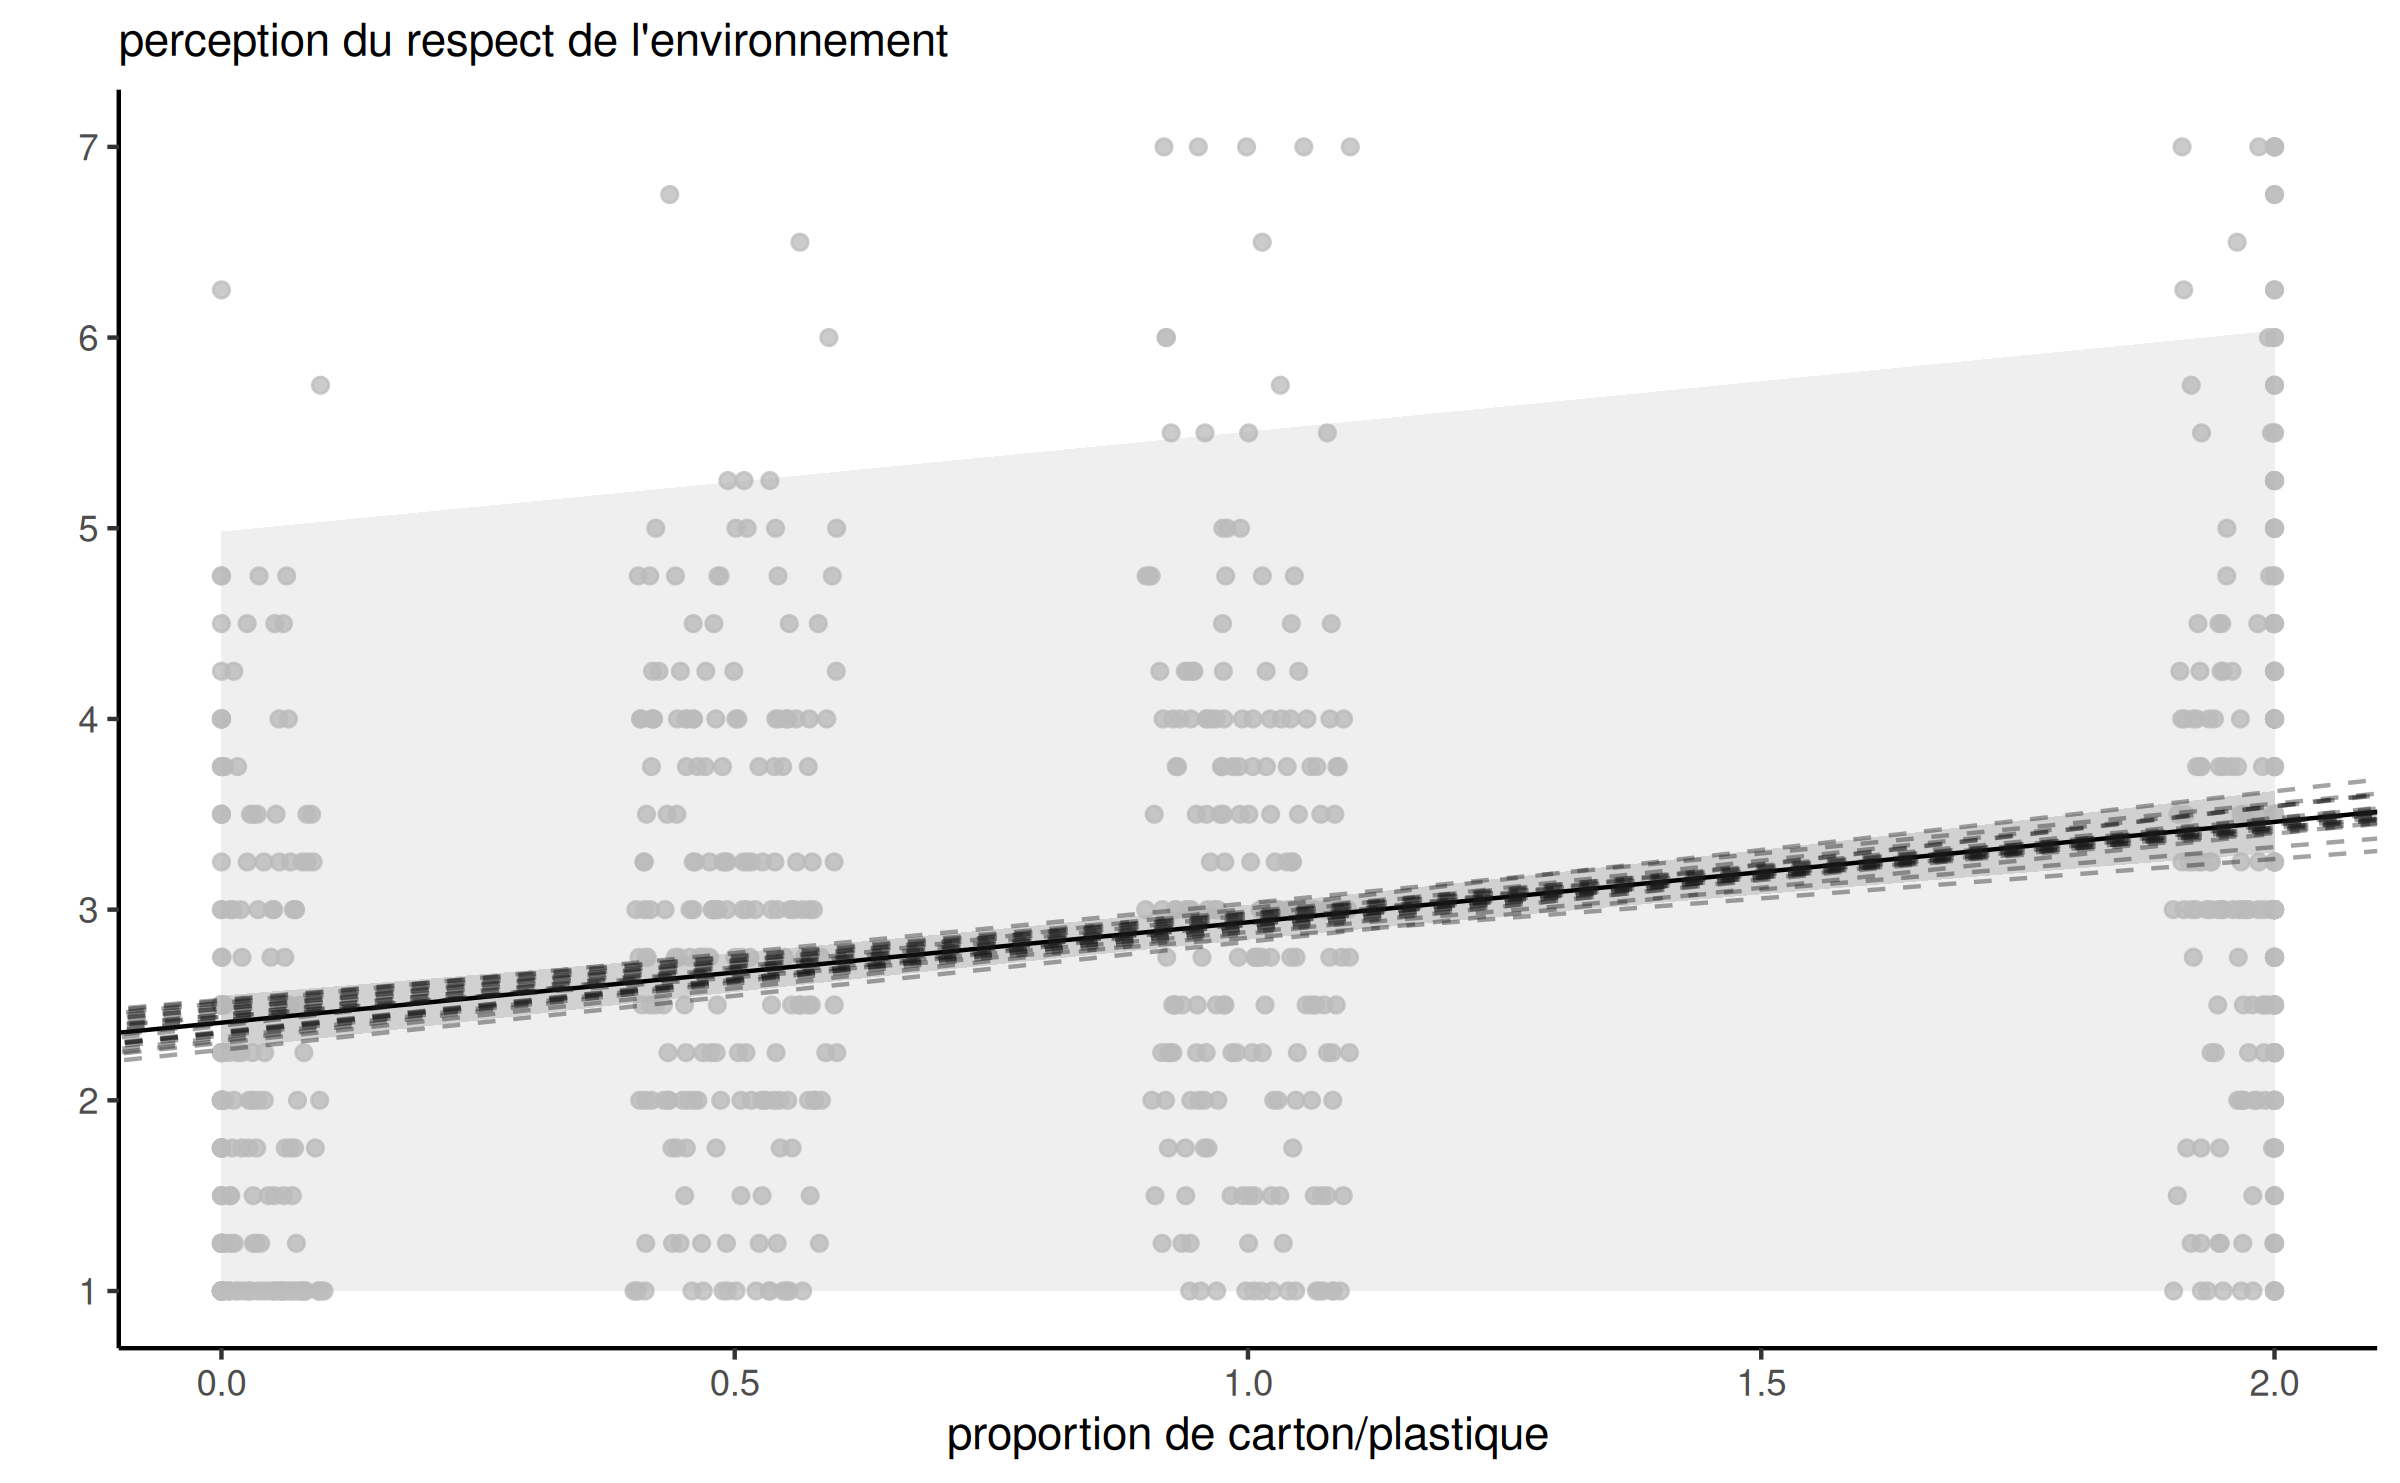
\includegraphics[width=0.85\textwidth,height=\textheight]{regression-lineaire_files/figure-pdf/fig-predinterval-1.png}

}

\caption{\label{fig-predinterval}Prédictions avec intervalles de
prédiction (à gauche) et intervalles de confiance pour la moyenne (à
droite) pour la régression linéaire simple de la perception du respect
de l'environnement (\texttt{pef}) en fonction de la \texttt{proportion}
de carton par rapport au plastique, avec des observations décalées
horizontalement. Le graphique montre les prédictions ainsi que les
intervalles de confiance ponctuels à 95 \% de la moyenne et des
prédictions individuelles. L'axe des ordonnées a été tronqué.}

\end{figure}%

Dans \textbf{R}, la fonction générique \texttt{predict} prend comme
arguments un modèle et une nouvelle base de données \texttt{newdata}
contenant un tableau avec la même structure que les données qui ont
servi à l'ajustement du modèle (à minima, les colonnes de variables
explicatives utilisées dans le modèle).

\begin{Shaded}
\begin{Highlighting}[]
\FunctionTok{data}\NormalTok{(SKD23\_S2A, }\AttributeTok{package =} \StringTok{"hecedsm"}\NormalTok{) }\CommentTok{\# charger les données}
\NormalTok{lm\_simple }\OtherTok{\textless{}{-}} \FunctionTok{lm}\NormalTok{(pef }\SpecialCharTok{\textasciitilde{}}\NormalTok{ proportion, }\AttributeTok{data =}\NormalTok{ SKD23\_S2A) }\CommentTok{\# régression linéaire simple}
\FunctionTok{predict}\NormalTok{(lm\_simple,}
        \AttributeTok{newdata =} \FunctionTok{data.frame}\NormalTok{(}\AttributeTok{proportion =} \FunctionTok{c}\NormalTok{(}\DecValTok{0}\NormalTok{, }\FloatTok{0.5}\NormalTok{, }\DecValTok{1}\NormalTok{, }\DecValTok{2}\NormalTok{)),}
        \AttributeTok{interval =} \StringTok{"prediction"}\NormalTok{) }\CommentTok{\# intervalles de prédiction}
\FunctionTok{predict}\NormalTok{(lm\_simple,}
        \AttributeTok{newdata =} \FunctionTok{data.frame}\NormalTok{(}\AttributeTok{proportion =} \FunctionTok{c}\NormalTok{(}\DecValTok{0}\NormalTok{, }\FloatTok{0.5}\NormalTok{, }\DecValTok{1}\NormalTok{, }\DecValTok{2}\NormalTok{)),}
        \AttributeTok{interval =} \StringTok{"confidence"}\NormalTok{) }\CommentTok{\# IC de confiance pour la moyenne}
\end{Highlighting}
\end{Shaded}

\begin{table}

\caption{\label{tbl-predints-soko}Prédictions avec intervalles de
prédiction (gauche) et intervalles de confiance pour la moyenne
(droite).}

\begin{minipage}{0.50\linewidth}

\begin{longtable}[]{@{}cccc@{}}
\caption{Intervalles de prédiction}\tabularnewline
\toprule\noalign{}
\texttt{proportion} & prédiction & borne inf. & borne sup. \\
\midrule\noalign{}
\endfirsthead
\toprule\noalign{}
\texttt{proportion} & prédiction & borne inf. & borne sup. \\
\midrule\noalign{}
\endhead
\bottomrule\noalign{}
\endlastfoot
0.0 & 2.41 & -0.168 & 4.98 \\
0.5 & 2.67 & 0.097 & 5.24 \\
1.0 & 2.93 & 0.361 & 5.51 \\
2.0 & 3.46 & 0.884 & 6.04 \\
\end{longtable}

\end{minipage}%
%
\begin{minipage}{0.50\linewidth}

\begin{longtable}[]{@{}ccc@{}}
\caption{Intervalles de confiance pour la moyenne}\tabularnewline
\toprule\noalign{}
moyenne & borne inf. & borne sup. \\
\midrule\noalign{}
\endfirsthead
\toprule\noalign{}
moyenne & borne inf. & borne sup. \\
\midrule\noalign{}
\endhead
\bottomrule\noalign{}
\endlastfoot
2.41 & 2.27 & 2.55 \\
2.67 & 2.57 & 2.77 \\
2.93 & 2.84 & 3.02 \\
3.46 & 3.30 & 3.62 \\
\end{longtable}

\end{minipage}%

\end{table}%

\end{example}

\section{Tests d'hypothèses}\label{tests-dhypothuxe8ses}

Les tests d'hypothèses dans les modèles linéaires et d'analyse de la
variance suivent la procédure usuelle: nous comparons deux modèles
emboîtés, dont l'un (le modèle nul) est une simplification d'un modèle
plus complexe (modèle alternatif) obtenu en imposant des restrictions
sur les coefficients de la moyenne.

Les tests de restrictions pour les composantes de \(\boldsymbol{\beta}\)
sont particulièrement intéressants. Les propriétés de l'estimateur du
maximum de vraisemblance pour les grands échantillons impliquent que
\begin{align*}
\widehat{\boldsymbol{\beta}} \stackrel{\cdot}{\sim}\mathsf{normale}_{p+1}\left\{\boldsymbol{\beta}, \sigma^2(\mathbf{X}^\top\mathbf{X})^{-1}\right\}
\end{align*} pour une taille d'échantillon suffisamment grande, et ce
résultat est exact si les observations sont normales. On peut aisément
obtenir les erreurs-type des coefficients en remplaçant \(\sigma^2\) par
un estimé; avec des données normales, on peut montrer que la somme du
carré des erreurs \(\mathsf{SC}_e \sim \sigma^2\chi^2_{n-p-1}\) et
\(\mathsf{SC}_e\) est indépendante de \(\widehat{\boldsymbol{\beta}}\).

Dans un contexte inférentiel, il est souvent important de tester si
l'effet d'une variable explicative est significatif : si \(x_j\) est
binaire ou continu, le test pour \(\mathscr{H}_0 : \beta_j=0\)
correspond à un effet marginal nul pour \(x_j\). Le modèle nul est une
régression linéaire dans laquelle nous supprimons la \((j+1)\)ème
colonne de \(\mathbf{X}\).

\begin{proposition}[Tests de Wald en régression
linéaire]\protect\hypertarget{prp-wald}{}\label{prp-wald}

Rappelons que la statistique du test de Wald pour l'hypothèse
\(\mathscr{H}_0: \beta_j=b\) est
\[W = \frac{\widehat{\beta}_j - b}{\mathsf{se}(\widehat{\beta}_j)}.\] La
statistique du test de Wald est rapportée par la plupart des logiciels
pour l'hypothèse \(b=0\). Puisque
\(\mathsf{Var}(\widehat{\beta}_j) = \sigma^2 [(\mathbf{X}^\top\mathbf{X})^{-1}]_{j,j}\),
nous pouvons estimer l'erreur type à partir de \(S^2\) et en déduire que
la distribution de \(W\) sous l'hypothèse nulle est
\(\mathsf{Student}(n-p-1)\). Cela explique la terminologie « \(t\)
values » dans le tableau \texttt{summary}. Outre les estimations des
coefficients, il est possible d'obtenir des intervalles de confiance
basés sur Wald pour \(\beta_j\), qui comme à l'accoutumée sont de la
forme
\(\widehat{\beta}_j \pm \mathfrak{t}_{n-p-1,\alpha/2} \mathsf{se}(\widehat{\beta}_j)\),
avec \(\mathfrak{t}_{n-p-1,\alpha/2}\) le quantile de niveau
\(1-\alpha/2\) d'une loi \(\mathsf{Student}({n-p-1})\).

\end{proposition}

\begin{example}[]\protect\hypertarget{exm-sokolova-simple-ttest}{}\label{exm-sokolova-simple-ttest}

Considérons les données de Exemple~\ref{exm-sokolova}. Si nous ajustons
le modèle de régression linéaire simple, nous pouvons extraire les
valeurs -\(p\) pour les tests de Wald ou tests-\(t\). Le test pour
l'ordonnée à l'origine est sans intérêt puisque les données sont
mesurées sur une échelle de 1 à 7, de sorte que la réponse moyenne
lorsque \texttt{proportion=0} ne peut être nulle. Le coefficient de
\texttt{proportion} suggère une tendance de 0.5 point par unité de
ratio, et il est significativement différent de zéro, ce qui indique que
le score \texttt{pef} change avec le ratio carton/plastique.

\begin{Shaded}
\begin{Highlighting}[]
\CommentTok{\# tests{-}t (Wald) pour beta=0 avec valeurs{-}p}
\FunctionTok{summary}\NormalTok{(lm\_simple)}\SpecialCharTok{$}\NormalTok{coefficients}
\CommentTok{\#\textgreater{}             Estimate Std. Error t value  Pr(\textgreater{}|t|)}
\CommentTok{\#\textgreater{} (Intercept)    2.407     0.0723   33.31 2.56e{-}153}
\CommentTok{\#\textgreater{} proportion     0.526     0.0618    8.51  8.40e{-}17}
\FunctionTok{confint}\NormalTok{(lm\_simple) }\CommentTok{\# intervalles de confiance pour betas}
\CommentTok{\#\textgreater{}             2.5 \% 97.5 \%}
\CommentTok{\#\textgreater{} (Intercept) 2.266  2.549}
\CommentTok{\#\textgreater{} proportion  0.405  0.648}
\end{Highlighting}
\end{Shaded}

\end{example}

Pour les variables catégorielles à plus de deux niveaux, tester si
\(\beta_j=0\) n'est généralement pas intéressant car le coefficient
représente la différence entre la catégorie \(x_j\) et la ligne de base
avec la paramétrisation du modèle en terme de contrastes (traitements):
ces deux catégories peuvent avoir une faible différence, mais la
variable catégorielle dans son ensemble peut toujours être un prédicteur
utile compte tenu des autres explications. L'hypothèse d'un contraste
nul est spécifique car elle implique un modèle nul dans lequel les
catégories sélectionnées sont fusionnées, ce qui dépend de la référence.
Nous souhaitons plutôt comparer un modèle dans lequel toutes les
variables sont présentes avec un modèle dans lequel la variable
explicative catégorielle est omise.

\begin{proposition}[Tests-\emph{F} pour comparaison de modèles
emboîtés]\protect\hypertarget{prp-ftest}{}\label{prp-ftest}

Considérons le modèle linéaire \emph{complet} qui contient \(p\)
variables explicatives, \begin{align*}
\mathbb{M}_1: Y=\beta_0+\beta_1 x_1 + \cdots + \beta_p x_p + \varepsilon.
\end{align*} Supposons sans perte de généralité que nous voulions tester
\(\mathscr{H}_0 : \beta_{k+1}=\beta_{k+2}=\cdots=\beta_p=0\) pour
\(k < p\) (on pourrait permuter les colonnes de la matrice du modèle
pour obtenir cette configuration). L'hypothèse globale spécifie que
\((p-k)\) des paramètres \(\beta\) sont nuls. Le \emph{modèle restreint}
correspondant à l'hypothèse nulle ne contient que les covariables pour
lesquelles \(\beta_j \neq 0\), \begin{align*}
\mathbb{M}_0: Y=\beta_0+\beta_1 x_1 + \cdots + \beta_k x_k + \varepsilon.
\end{align*} Soit \(\mathsf{SC}_e(\mathbb{M}_1)\) la somme du carré des
résidus du modèle complet \(\mathbb{M}_1\), \begin{align*}
\mathsf{SC}_e(\mathbb{M}_1)=\sum_{i=1}^n (Y_i-\widehat{Y}_i^{\mathbb{M}_1})^2,
\end{align*} où \(\hat{Y}_i^{\mathbb{M}_1}\) est la \(i\)e valeur
ajustée du modèle \(\mathbb{M}_1\). On définit de la même façon la somme
du carré des résidus, \(\mathsf{SC}_e(\mathbb{M}_0)\), pour le modèle
\(\mathbb{M}_0\). Logiquement,
\(\mathsf{SC}_e(\mathbb{M}_0) \geq \mathsf{SC}_e(\mathbb{M}_1)\).

La statistique \(F\) est \begin{align*}
F=\frac{\{\mathsf{SC}_e(\mathbb{M}_0)-\mathsf{SC}_e(\mathbb{M}_1)\}/(p-k)}{\mathsf{SC}_e(\mathbb{M}_1)/(n-p-1)}.
\end{align*} Sous \(\mathscr{H}_0\), la statistique \(F\) suit une loi
de Fisher (Définition~\ref{def-loiF}) avec \((p-k)\) et \((n-p-1)\)
degrés de liberté, \(\mathsf{Fisher}(p-k, n-p-1)\). Les degrés de
libertés du numérateur, \(p-k\), indiquent le nombre de restrictions ou
la différence du nombre de paramètres, tandis que celle du dénominateur,
\(n-p-1\) est la taille de l'échantillons moins le nombre de paramères
pour la moyenne du modèle \(\mathbb{M}_1\).

\end{proposition}

Quand la \(j\)e variable explicative est continue ou binaire, le test
\(F\) est équivalent au test \(t\) pour \(\beta_j=0\). En effet, la
statistique \(F\) est le carré de la statistique de Wald, et ils mènent
à la même inférence --- les valeurs-\(p\) sont identiques. Bien qu'il
soit rapporté dans les tableaux, le test pour \(\beta_0=0\) n'est pas
intéressant; nous conservons l'ordonnée à l'origine uniquement pour
centrer les résidus.

\begin{refremark}[Tests \emph{F} versus test du rapport de
vraisemblance]
Pour la régression linéaire normale, le test du rapport de vraisemblance
pour comparer les modèles \(\mathbb{M}_1\) et \(\mathbb{M}_0\) est une
fonction de la somme des carrés des résidus: la formule habituelle se
simplifie à \begin{align*}
R &= 2( \ell_{\mathbb{M}_1} - \ell_{\mathbb{M}_0}) \\&= n\ln\{\mathsf{SC}_e(\mathbb{M}_0)/\mathsf{SC}_e(\mathbb{M}_1)\}\\
&= n \ln \left( 1+ \frac{p-k}{n-p-1}F\right)
\end{align*} Le test du rapport de vraisemblance et les tests \(F\) sont
liés par une transformation monotone, et nous pouvons utiliser la
distribution \(\mathsf{Fisher}\) à des fins de comparaison, plutôt que
l'approximation \(\chi^2\) pour grand échantillon. Les tests \(t\) et
\(F\) présentés ci-dessus pourraient donc tous deux être considérés
comme des cas particuliers de \href{@sec-testsvrais}{tests de rapport de
vraisemblance}, mais en utilisant Student-\(t\) contre la distribution
normale lorsque \(p-k=1\), et \(\mathsf{Fisher}\) contre \(\chi^2\)
lorsque \(p-k \ge 1\). Lorsque \(n\) est grand, les résultats sont à peu
près les mêmes.

\label{rem-lrtvsF}

\end{refremark}

\subsection{Contrastes}\label{contrastes}

Supposons que nous effectuions une analyse de la variance et que le test
\(F\) pour l'hypothèse nulle (globale) selon laquelle les moyennes de
tous les groupes sont égales soit très élevé: nous rejetons l'hypothèse
nulle en faveur de l'alternative, qui stipule qu'au moins une des
moyennes du groupe est différente. La question suivante sera de savoir
où se situent ces différences. En effet, dans un contexte expérimental,
cela implique qu'une ou plusieurs manipulations ont un effet différent
des autres sur la réponse moyenne. Souvent, cela n'est pas intéressant
en soi: nous pourrions être intéressés par la comparaison de différentes
options par rapport à un groupe de contrôle ou déterminer si des
combinaisons spécifiques fonctionnent mieux que séparément, ou trouver
le meilleur traitement en comparant toutes les paires.

La question scientifique qui a justifié l'expérience peut conduire à un
ensemble spécifique d'hypothèses, qui peuvent être formulées par les
chercheurs comme des comparaisons entre les moyennes de différents
sous-groupes. Nous pouvons normalement les exprimer sous la forme de
\textbf{contrastes}. Si le test global \(F\) pour l'égalité des moyennes
est équivalent à une pièce faiblement éclairée, les contrastes sont
comparables à des projecteurs qui permettent de mettre l'accent sur des
aspects particuliers des différences entre les traitements.
Formellement, un contraste est une combinaison linéaire de moyennes: en
clair, cela signifie que nous attribuons un poids à chaque moyenne de
groupe et que nous les additionnons, puis que nous comparons ce résumé à
une valeur postulée \(a\), généralement zéro.

Les contrastes encodent la question de recherche : si \(c_i\) représente
le poids de la moyenne du groupe \(\mu_i\) \((i=1, \ldots, K)\), alors
nous pouvons écrire le contraste comme
\(C = c_1 \mu_1 + \cdots + c_K \mu_K\) avec l'hypothèse nulle
\(\mathscr{H}_0 : C=a\) pour une alternative bilatérale. L'estimation du
contraste linéaire est obtenue en remplaçant la moyenne inconnue de la
population \(\mu_i\) par la moyenne de l'échantillon de ce groupe,
\(\widehat{\mu}_i = \overline{y}_{i}\). Nous pouvons facilement obtenir
l'erreur type de la combinaison linéaire \(C\). La formule, l'erreur
type, en supposant une taille de sous-échantillon de
\(n_1, \ldots, n_K\) et une variance commune \(\sigma^2\), est la racine
carrée de \begin{align*}
\mathsf{Va}(\widehat{C}) = \widehat{\sigma}^2\left(\frac{c_1^2}{n_1} + \cdots + \frac{c_K^2}{n_K}\right).
\end{align*} Nous pouvons alors construire une statistique \(t\) comme
d'habitude en examinant la différence entre notre valeur postulée et la
moyenne pondérée observée, convenablement normalisée. Si le test global
\(F\) conduit au rejet de la valeur nulle, il existe au moins un
contraste significatif au même niveau. Lorsque les vecteurs de contraste
sont orthogonaux, les tests ne sont pas corrélés. Mathématiquement, si
nous laissons \(c_{i}\) et \(c^{*}_{i}\) désigner les poids attachés à
la moyenne du groupe \(i\) comprenant \(n_i\) observations, les
contrastes sont orthogonaux si
\(c_{1}c^{*}_{1}/n_1 + \cdots + c_{K}c^{*}_K/n_K = 0\) ; si
l'échantillon est équilibré avec le même nombre d'observations dans
chaque groupe, \(n/K = n_1 =\cdots = n_K\), nous pouvons considérer le
produit scalaire des deux vecteurs de contrastes et négliger la taille
des sous-échantillons.

Si nous avons \(K\) groupes, il y a \(K-1\) contrastes pour les
différences deux à deux, le dernier étant capturé par la moyenne de
l'échantillon pour l'effet global. Si nous nous intéressons uniquement à
la différence entre groupes (par opposition à l'effet global de tous les
traitements), nous imposons une contrainte de somme à zéro sur les
poids, de sorte que \(c_1 + \cdots + c_K=0\).

\subsection{Exemples de tests}\label{exemples-de-tests}

\begin{example}[Test du montant des
dons]\protect\hypertarget{exm-moonvaepps-test}{}\label{exm-moonvaepps-test}

Considérons l'Exemple~\ref{exm-moon}, dans lequel nous testons les
différences entre les montants libres (\texttt{open-ended}) et les
montants suggérés (\texttt{quantity}). Le test qui nous intéresse est
\(\mathscr{H}_0 : \beta_1=0\), où
\(\beta_1=\mu_{\texttt{oe}} - \mu_{\texttt{qty}}\) est la différence
moyenne entre les groupes. Outre le fait que la différence est
statistiquement significative au niveau de 5 \%, nous voulons également
rapporter les \textbf{moyennes marginales}, qui, lorsque nous avons une
seule variable explicative catégorielle dans le modèle linéaire, est la
moyenne empirique de chaque sous-groupe.

\begin{Shaded}
\begin{Highlighting}[]
\FunctionTok{data}\NormalTok{(}\StringTok{"MV23\_S1"}\NormalTok{, }\AttributeTok{package =} \StringTok{"hecedsm"}\NormalTok{)}
\NormalTok{MV23\_S1 }\OtherTok{\textless{}{-}}\NormalTok{ MV23\_S1 }\SpecialCharTok{|\textgreater{}}
\NormalTok{    dplyr}\SpecialCharTok{::}\FunctionTok{mutate}\NormalTok{(}\AttributeTok{amount2 =} \FunctionTok{ifelse}\NormalTok{(}\FunctionTok{is.na}\NormalTok{(amount), }\DecValTok{0}\NormalTok{, amount))}
\NormalTok{linmod\_MV23 }\OtherTok{\textless{}{-}} \FunctionTok{lm}\NormalTok{(amount2 }\SpecialCharTok{\textasciitilde{}}\NormalTok{ condition, }\AttributeTok{data =}\NormalTok{ MV23\_S1)}
\CommentTok{\# Test Wald avec coefficients}
\FunctionTok{summary}\NormalTok{(linmod\_MV23)}
\CommentTok{\#\textgreater{} }
\CommentTok{\#\textgreater{} Call:}
\CommentTok{\#\textgreater{} lm(formula = amount2 \textasciitilde{} condition, data = MV23\_S1)}
\CommentTok{\#\textgreater{} }
\CommentTok{\#\textgreater{} Residuals:}
\CommentTok{\#\textgreater{}    Min     1Q Median     3Q    Max }
\CommentTok{\#\textgreater{}  {-}8.70  {-}6.77  {-}1.77   3.23  18.23 }
\CommentTok{\#\textgreater{} }
\CommentTok{\#\textgreater{} Coefficients:}
\CommentTok{\#\textgreater{}                   Estimate Std. Error t value Pr(\textgreater{}|t|)    }
\CommentTok{\#\textgreater{} (Intercept)          6.771      0.377   17.95   \textless{}2e{-}16 ***}
\CommentTok{\#\textgreater{} conditionquantity    1.929      0.517    3.73   0.0002 ***}
\CommentTok{\#\textgreater{} {-}{-}{-}}
\CommentTok{\#\textgreater{} Signif. codes:  0 \textquotesingle{}***\textquotesingle{} 0.001 \textquotesingle{}**\textquotesingle{} 0.01 \textquotesingle{}*\textquotesingle{} 0.05 \textquotesingle{}.\textquotesingle{} 0.1 \textquotesingle{} \textquotesingle{} 1}
\CommentTok{\#\textgreater{} }
\CommentTok{\#\textgreater{} Residual standard error: 7.61 on 867 degrees of freedom}
\CommentTok{\#\textgreater{} Multiple R{-}squared:  0.0158, Adjusted R{-}squared:  0.0147 }
\CommentTok{\#\textgreater{} F{-}statistic: 13.9 on 1 and 867 DF,  p{-}value: 0.000205}
\CommentTok{\# ANOVA avec tests F}
\FunctionTok{anova}\NormalTok{(linmod\_MV23)}
\CommentTok{\#\textgreater{} Analysis of Variance Table}
\CommentTok{\#\textgreater{} }
\CommentTok{\#\textgreater{} Response: amount2}
\CommentTok{\#\textgreater{}            Df Sum Sq Mean Sq F value Pr(\textgreater{}F)    }
\CommentTok{\#\textgreater{} condition   1    805     805    13.9 0.0002 ***}
\CommentTok{\#\textgreater{} Residuals 867  50214      58                   }
\CommentTok{\#\textgreater{} {-}{-}{-}}
\CommentTok{\#\textgreater{} Signif. codes:  0 \textquotesingle{}***\textquotesingle{} 0.001 \textquotesingle{}**\textquotesingle{} 0.01 \textquotesingle{}*\textquotesingle{} 0.05 \textquotesingle{}.\textquotesingle{} 0.1 \textquotesingle{} \textquotesingle{} 1}
\CommentTok{\# Moyennes marginales}
\NormalTok{(emm }\OtherTok{\textless{}{-}}\NormalTok{ emmeans}\SpecialCharTok{::}\FunctionTok{emmeans}\NormalTok{(linmod\_MV23, }\AttributeTok{spec =} \StringTok{"condition"}\NormalTok{))}
\CommentTok{\#\textgreater{}  condition  emmean    SE  df lower.CL upper.CL}
\CommentTok{\#\textgreater{}  open{-}ended   6.77 0.377 867     6.03     7.51}
\CommentTok{\#\textgreater{}  quantity     8.70 0.354 867     8.01     9.40}
\CommentTok{\#\textgreater{} }
\CommentTok{\#\textgreater{} Confidence level used: 0.95}
\NormalTok{emm }\SpecialCharTok{|\textgreater{}}\NormalTok{ emmeans}\SpecialCharTok{::}\FunctionTok{contrast}\NormalTok{(}\AttributeTok{method =} \StringTok{"pairwise"}\NormalTok{) }\CommentTok{\# vecteur de contraste (1,{-}1)}
\CommentTok{\#\textgreater{}  contrast                estimate    SE  df t.ratio p.value}
\CommentTok{\#\textgreater{}  (open{-}ended) {-} quantity    {-}1.93 0.517 867  {-}3.730  0.0002}
\end{Highlighting}
\end{Shaded}

\end{example}

\begin{example}[Tests et contrastes pour les méthodes de compréhension
de la
lecture]\protect\hypertarget{exm-teachingtoread}{}\label{exm-teachingtoread}

Nous examinons maintenant les tests pour
l'Exemple~\ref{exm-teaching-baumann} et
l'Exemple~\ref{exm-baumann-dummies}, avec une covariable en plus.
L'objectif de Baumann, Seifert-Kessell, et Jones
(\citeproc{ref-Baumann:1992}{1992}) était de faire une comparaison
particulière entre des groupes de traitement. Selon le résumé de
l'article:

\begin{quote}
Les analyses quantitatives principales comportaient deux contrastes
orthogonaux planifiés: l'effet de l'enseignement (TA + DRTA vs.~2 x DR)
et l'intensité de l'enseignement (TA vs.~DRTA).
\end{quote}

Avec un modèle pré-post, nous allons comparer les moyennes pour une
valeur commune de \texttt{pretest1}, ci-dessous la moyenne globale du
score \texttt{pretest1}.

\begin{Shaded}
\begin{Highlighting}[]
\FunctionTok{library}\NormalTok{(emmeans) }\CommentTok{\# moyennes marginales}
\FunctionTok{data}\NormalTok{(BSJ92, }\AttributeTok{package =} \StringTok{"hecedsm"}\NormalTok{)}
\NormalTok{mod\_post }\OtherTok{\textless{}{-}} \FunctionTok{lm}\NormalTok{(posttest1 }\SpecialCharTok{\textasciitilde{}}\NormalTok{ group }\SpecialCharTok{+}\NormalTok{ pretest1,}
               \AttributeTok{data =}\NormalTok{ BSJ92)}
\NormalTok{mod\_post0 }\OtherTok{\textless{}{-}} \FunctionTok{lm}\NormalTok{(posttest1 }\SpecialCharTok{\textasciitilde{}}\NormalTok{ pretest1,}
               \AttributeTok{data =}\NormalTok{ BSJ92)}
\FunctionTok{anova}\NormalTok{(mod\_post0, mod\_post) }\CommentTok{\# tests F}
\CommentTok{\#\textgreater{} Analysis of Variance Table}
\CommentTok{\#\textgreater{} }
\CommentTok{\#\textgreater{} Model 1: posttest1 \textasciitilde{} pretest1}
\CommentTok{\#\textgreater{} Model 2: posttest1 \textasciitilde{} group + pretest1}
\CommentTok{\#\textgreater{}   Res.Df RSS Df Sum of Sq    F   Pr(\textgreater{}F)    }
\CommentTok{\#\textgreater{} 1     64 509                               }
\CommentTok{\#\textgreater{} 2     62 365  2       143 12.2 0.000035 ***}
\CommentTok{\#\textgreater{} {-}{-}{-}}
\CommentTok{\#\textgreater{} Signif. codes:  0 \textquotesingle{}***\textquotesingle{} 0.001 \textquotesingle{}**\textquotesingle{} 0.01 \textquotesingle{}*\textquotesingle{} 0.05 \textquotesingle{}.\textquotesingle{} 0.1 \textquotesingle{} \textquotesingle{} 1}
\NormalTok{emmeans\_post }\OtherTok{\textless{}{-}} \FunctionTok{emmeans}\NormalTok{(}\AttributeTok{object =}\NormalTok{ mod\_post,}
                        \AttributeTok{specs =} \StringTok{"group"}\NormalTok{)}
\end{Highlighting}
\end{Shaded}

Le résultat du tableau d'analyse de la variance montre qu'il y a bien
des différences entre les groupes. On peut donc s'intéresser aux
moyennes marginales estimées, qui sont la moyenne de chaque groupe.

\begin{longtable}[]{@{}lrrrrr@{}}

\caption{\label{tbl-print-pairwise-baumann}Moyennes estimées des groupes
avec erreurs-types et intervalles de confiance à 95 \% pour le post-test
1 pour un score moyen au pré-test 1.}

\tabularnewline

\toprule\noalign{}
termes & moyennes & erreur-type & ddl & borne inf. & borne sup. \\
\midrule\noalign{}
\endhead
\bottomrule\noalign{}
\endlastfoot
DR & 6.19 & 0.52 & 62 & 5.14 & 7.23 \\
DRTA & 9.81 & 0.52 & 62 & 8.78 & 10.85 \\
TA & 8.22 & 0.52 & 62 & 7.18 & 9.27 \\

\end{longtable}

Les deux hypothèses et contrastes de Baumann, Seifert-Kessell, et Jones
(\citeproc{ref-Baumann:1992}{1992}) sont
\(\mathscr{H}_0: \mu_{\mathrm{TA}} + \mu_{\mathrm{DRTA}} = 2 \mu_{\mathrm{DRA}}\)
ou \begin{align*}
\mathscr{H}_0: - 2 \mu_{\mathrm{DR}} + \mu_{\mathrm{DRTA}} + \mu_{\mathrm{TA}} = 0.
\end{align*} avec poids \(c_1=(-2, 1, 1)\); l'ordre des niveaux de
traitement est (\(\mathrm{DRA}\), \(\mathrm{DRTA}\), \(\mathrm{TA}\)) et
ce dernier doit correspond à celui des poids pour les contrastes. Ces
derniers donnent les mêmes tests à multiple non-nul près, donc \(ac_1\),
\(a \neq 0\) donne un résultat équivalent, par exemple \((2, -1, -1)\)
ou \((1, -1/2, -1/2)\) fonctionnent. Si les estimations changent, les
erreurs-types sont ajustées d'autant. Un vecteur de contrastes pour
\(\mathscr{H}_0:  \mu_{\mathrm{TA}} = \mu_{\mathrm{DRTA}}\) est (\(0\),
\(-1\), \(1\)): le zéro apparaît parce que la première composante,
\(\mathrm{DRA}\) n'apparaît pas. Les deux contrastes sont orthogonaux
puisque \((-2 \times 0) + (1 \times -1) + (1 \times 1) = 0\).

\begin{Shaded}
\begin{Highlighting}[]
\CommentTok{\# Identifier l\textquotesingle{}ordre de niveau du facteur}
\FunctionTok{with}\NormalTok{(BSJ92, }\FunctionTok{levels}\NormalTok{(group))}
\CommentTok{\#\textgreater{} [1] "DR"   "DRTA" "TA"}
\CommentTok{\# DR, DRTA, TA (alphabetical)}
\NormalTok{contrastes\_list }\OtherTok{\textless{}{-}} \FunctionTok{list}\NormalTok{(}
  \CommentTok{\# Contrastes: combo linéaire de moyennes,}
  \CommentTok{\# la somme des coefficients doit être nulle}
  \StringTok{"C1: moy(DRTA+TA) vs DR"} \OtherTok{=} \FunctionTok{c}\NormalTok{(}\SpecialCharTok{{-}}\DecValTok{1}\NormalTok{, }\FloatTok{0.5}\NormalTok{, }\FloatTok{0.5}\NormalTok{),}
  \StringTok{"C2: DRTA vs TA"} \OtherTok{=} \FunctionTok{c}\NormalTok{(}\DecValTok{0}\NormalTok{, }\DecValTok{1}\NormalTok{, }\SpecialCharTok{{-}}\DecValTok{1}\NormalTok{)}
\NormalTok{)}
\NormalTok{contrastes\_post }\OtherTok{\textless{}{-}}
  \FunctionTok{contrast}\NormalTok{(}\AttributeTok{object =}\NormalTok{ emmeans\_post,}
           \AttributeTok{method =}\NormalTok{ contrastes\_list)}
\NormalTok{contrastes\_summary\_post }\OtherTok{\textless{}{-}} \FunctionTok{summary}\NormalTok{(contrastes\_post)}
\end{Highlighting}
\end{Shaded}

\begin{longtable}[t]{lrrrrr}

\caption{\label{tbl-print-contrasts}Contrastes estimés pour le post-test
1.}

\tabularnewline

\toprule
contraste & estimation & erreur-type & ddl & stat & valeur-p\\
\midrule
C1: moy(DRTA+TA) vs DR & 2.83 & 0.64 & 62 & 4.40 & 0.00\\
C2: DRTA vs TA & 1.59 & 0.73 & 62 & 2.17 & 0.03\\
\bottomrule

\end{longtable}

Nous pouvons examiner ces différences: puisque \texttt{DRTA} contre
\texttt{TA} est une différence par paire, nous aurions pu obtenir la
statistique \(t\) directement à partir des contrastes deux à deux en
utilisant \texttt{pairs(emmeans\_post)}.

Quelle est la conclusion de notre analyse des contrastes? Il semble que
les méthodes impliquant la réflexion à haute voix aient un impact
important sur la compréhension de la lecture par rapport à la seule
lecture dirigée. Les preuves ne sont pas aussi solides lorsque nous
comparons la méthode qui combine la lecture dirigée, l'activité de
réflexion et la réflexion à haute voix, mais la différence est néanmoins
significative à niveau 5\%.

\begin{Shaded}
\begin{Highlighting}[]
\CommentTok{\# Extraire les coefficients et les erreurs{-}type}
\NormalTok{beta\_pre }\OtherTok{\textless{}{-}} \FunctionTok{coefficients}\NormalTok{(mod\_post)[}\StringTok{\textquotesingle{}pretest1\textquotesingle{}}\NormalTok{]}
\NormalTok{se\_pre }\OtherTok{\textless{}{-}} \FunctionTok{sqrt}\NormalTok{(}\FunctionTok{c}\NormalTok{(}\FunctionTok{vcov}\NormalTok{(mod\_post)[}\StringTok{\textquotesingle{}pretest1\textquotesingle{}}\NormalTok{, }\StringTok{\textquotesingle{}pretest1\textquotesingle{}}\NormalTok{]))}
\NormalTok{wald }\OtherTok{\textless{}{-}}\NormalTok{ (beta\_pre }\SpecialCharTok{{-}} \DecValTok{1}\NormalTok{)}\SpecialCharTok{/}\NormalTok{se\_pre }\CommentTok{\# test de Wald directionnel}
\CommentTok{\# Valeur{-}p basée sur la référence nulle Student{-}t avec n{-}p{-}1 ddl}
\NormalTok{pval }\OtherTok{\textless{}{-}} \DecValTok{2}\SpecialCharTok{*}\FunctionTok{pt}\NormalTok{(}\FunctionTok{abs}\NormalTok{(wald), }\AttributeTok{df =}\NormalTok{ mod\_post}\SpecialCharTok{$}\NormalTok{df.residual, }\AttributeTok{lower.tail =} \ConstantTok{FALSE}\NormalTok{)}
\CommentTok{\# Comparaison de modèles emboîtés avec appel à \textquotesingle{}anova\textquotesingle{}}
\NormalTok{mod0 }\OtherTok{\textless{}{-}} \FunctionTok{lm}\NormalTok{(posttest1 }\SpecialCharTok{\textasciitilde{}} \FunctionTok{offset}\NormalTok{(pretest1) }\SpecialCharTok{+}\NormalTok{ group, }\AttributeTok{data =}\NormalTok{ BSJ92)}
\CommentTok{\# Le décalage (\textasciigrave{}offset\textasciigrave{}) fixe le terme, ce qui équivaut à un coefficient de 1.}
\NormalTok{aov\_tab }\OtherTok{\textless{}{-}} \FunctionTok{anova}\NormalTok{(mod0, mod\_post)}
\end{Highlighting}
\end{Shaded}

Une autre hypothèse potentielle intéressante consiste à tester si le
coefficient de \texttt{pretest1} est égal à l'unité. Cela équivaut à
l'hypothèse \(b=1\) pour le test de Wald,
\(w = (\widehat{\beta}_{\texttt{pretest1}}-1)/\mathsf{se}(\widehat{\beta}_{\texttt{pretest1}})= -3.024\),
ou bien une comparaison de modèles avec le test \(F\) via
\texttt{anova}, qui donne une statistique de test de \(F=9.143.\) On
peut montrer que si \(Z \sim \mathsf{Student}(\nu)\), alors
\(Z^2 \sim \mathsf{Fisher}(1, \nu)\), il s'ensuit que les deux tests
sont équivalents et que les valeurs-\(p\) sont exactement les mêmes.

\end{example}

\begin{example}[Tests et contrastes pour l'effet de l'emballage carton
sur la
perception]\protect\hypertarget{exm-paperorplastic}{}\label{exm-paperorplastic}

Soit \(\mu_{0}, \mu_{0.5}, \mu_{1}, \mu_2\) la vraie moyenne du score
PEF en fonction de la proportion de carton pour les données de
Exemple~\ref{exm-sokolova}. Plusieurs tests pourraient être intéressants
ici, mais nous nous concentrons sur les contrastes effectués par les
auteurs et sur un test d'hypothèse de linéarité en fonction de la
proportion de plastique. Pour ce dernier, nous pouvons comparer le
modèle de régression linéaire (dans lequel le score PEF augmente
linéairement avec la proportion de carton par rapport au plastique),
\begin{align*}
 \mathsf{E}(\texttt{pef} \mid \texttt{proportion}) = \beta_0 + \beta_1\texttt{proportion},
 \end{align*} au modèle d'analyse de variance qui permet à chacun des
quatre groupes d'avoir des moyennes différentes. \begin{align*}
 &\mathsf{E}(\texttt{pef} \mid \texttt{proportion}) = \alpha_0 + \alpha_1 \mathbf{1}_{\texttt{proportion}=0.5} \\&\quad + \alpha_2 \mathbf{1}_{\texttt{proportion}=1} + \alpha_3\mathbf{1}_{\texttt{proportion}=2}.
\end{align*} Si on veut obtenir l'hypothèse nulle en terme de
contraintes sur les paramètres \(\boldsymbol{\alpha}\), on trouve
\begin{align*}
\mu_0 &= \beta_0=\alpha_0 \\
\mu_{0.5} &= \beta_0 + 0.5 \beta_1 = \alpha_0 + \alpha_1\\
\mu_1 &= \beta_0 + \beta_1 = \alpha_0 + \alpha_2 \\
\mu_2 &= \beta_0 + 2 \beta_1= \alpha_0 + \alpha_3.
\end{align*} Le test comparant la régression linéaire simple à l'analyse
de la variance impose deux restrictions simultanées, avec
\(\mathscr{H}_0 : \alpha_3 = 2\alpha_2= 4\alpha_1\), de sorte que la
distribution nulle est \(\mathsf{Fisher}(2, 798)\) ou approximativement
\(\chi^2_2\).

\begin{Shaded}
\begin{Highlighting}[]
\FunctionTok{data}\NormalTok{(SKD23\_S2A, }\AttributeTok{package =} \StringTok{"hecedsm"}\NormalTok{)}
\NormalTok{linmod }\OtherTok{\textless{}{-}} \FunctionTok{lm}\NormalTok{(pef }\SpecialCharTok{\textasciitilde{}}\NormalTok{ proportion, }\AttributeTok{data =}\NormalTok{ SKD23\_S2A)}
\FunctionTok{coef}\NormalTok{(linmod) }\CommentTok{\# extraire coefficients}
\CommentTok{\#\textgreater{} (Intercept)  proportion }
\CommentTok{\#\textgreater{}       2.407       0.526}
\CommentTok{\# ANOVA à un facteur}
\NormalTok{anovamod }\OtherTok{\textless{}{-}} \FunctionTok{lm}\NormalTok{(pef }\SpecialCharTok{\textasciitilde{}} \FunctionTok{factor}\NormalTok{(proportion),}
               \AttributeTok{data =}\NormalTok{ SKD23\_S2A)}
\CommentTok{\# Comparer les deux modèles emboîtés}
\FunctionTok{anova}\NormalTok{(linmod, anovamod) }\CommentTok{\# est{-}ce que l\textquotesingle{}effet est linéaire?}
\CommentTok{\#\textgreater{} Analysis of Variance Table}
\CommentTok{\#\textgreater{} }
\CommentTok{\#\textgreater{} Model 1: pef \textasciitilde{} proportion}
\CommentTok{\#\textgreater{} Model 2: pef \textasciitilde{} factor(proportion)}
\CommentTok{\#\textgreater{}   Res.Df  RSS Df Sum of Sq    F  Pr(\textgreater{}F)    }
\CommentTok{\#\textgreater{} 1    800 1373                              }
\CommentTok{\#\textgreater{} 2    798 1343  2      29.3 8.69 0.00018 ***}
\CommentTok{\#\textgreater{} {-}{-}{-}}
\CommentTok{\#\textgreater{} Signif. codes:  0 \textquotesingle{}***\textquotesingle{} 0.001 \textquotesingle{}**\textquotesingle{} 0.01 \textquotesingle{}*\textquotesingle{} 0.05 \textquotesingle{}.\textquotesingle{} 0.1 \textquotesingle{} \textquotesingle{} 1}
\CommentTok{\# Test avec code alternatif (poids pour chaque coefficient)}
\NormalTok{car}\SpecialCharTok{::}\FunctionTok{linearHypothesis}\NormalTok{(}\AttributeTok{model =}\NormalTok{ anovamod,}
   \AttributeTok{hypothesis =} \FunctionTok{rbind}\NormalTok{(}\FunctionTok{c}\NormalTok{(}\DecValTok{0}\NormalTok{, }\SpecialCharTok{{-}}\DecValTok{2}\NormalTok{, }\DecValTok{1}\NormalTok{, }\DecValTok{0}\NormalTok{),}
                      \FunctionTok{c}\NormalTok{(}\DecValTok{0}\NormalTok{, }\DecValTok{0}\NormalTok{, }\SpecialCharTok{{-}}\DecValTok{2}\NormalTok{, }\DecValTok{1}\NormalTok{)))}
\CommentTok{\#\textgreater{} Linear hypothesis test}
\CommentTok{\#\textgreater{} }
\CommentTok{\#\textgreater{} Hypothesis:}
\CommentTok{\#\textgreater{} {-} 2 factor(proportion)0.5  + factor(proportion)1 = 0}
\CommentTok{\#\textgreater{} {-} 2 factor(proportion)1  + factor(proportion)2 = 0}
\CommentTok{\#\textgreater{} }
\CommentTok{\#\textgreater{} Model 1: restricted model}
\CommentTok{\#\textgreater{} Model 2: pef \textasciitilde{} factor(proportion)}
\CommentTok{\#\textgreater{} }
\CommentTok{\#\textgreater{}   Res.Df  RSS Df Sum of Sq    F  Pr(\textgreater{}F)    }
\CommentTok{\#\textgreater{} 1    800 1373                              }
\CommentTok{\#\textgreater{} 2    798 1343  2      29.3 8.69 0.00018 ***}
\CommentTok{\#\textgreater{} {-}{-}{-}}
\CommentTok{\#\textgreater{} Signif. codes:  0 \textquotesingle{}***\textquotesingle{} 0.001 \textquotesingle{}**\textquotesingle{} 0.01 \textquotesingle{}*\textquotesingle{} 0.05 \textquotesingle{}.\textquotesingle{} 0.1 \textquotesingle{} \textquotesingle{} 1}
\end{Highlighting}
\end{Shaded}

Le résultat montre que les tests \(F\) et les valeurs-\(p\) sont
identiques, que l'on impose les contraintes manuellement ou que l'on
soumette simplement les deux modèles imbriqués à la méthode
\texttt{anova}.

Les auteurs souhaitaient comparer zéro carton avec d'autres choix: nous
nous intéressons aux différences par paire, mais uniquement par rapport
à la référence \(\mu_{0}\): \begin{align*}
\mu_0 = \mu_{0.5}  & \iff 1\mu_0 - 1\mu_{0.5} + 0\mu_{1} + 0 \mu_{2} = 0\\
\mu_0 = \mu_{1} & \iff 1\mu_0 + 0\mu_{0.5} -1\mu_{1} + 0 \mu_{2} = 0\\
\mu_0 = \mu_{2} & \iff 1\mu_0 + 0\mu_{0.5} + 0\mu_{1} -1 \mu_{2} = 0.
\end{align*} Les vecteurs de poids pour les contrastes linéaires sont
\((1, -1, 0, 0)\), \((1, 0, -1, 0)\) et \((1, 0, 0, -1)\) pour les
moyennes marginales.

\begin{Shaded}
\begin{Highlighting}[]
\NormalTok{moymarg }\OtherTok{\textless{}{-}}\NormalTok{ anovamod }\SpecialCharTok{|\textgreater{}}
\NormalTok{  emmeans}\SpecialCharTok{::}\FunctionTok{emmeans}\NormalTok{(}\AttributeTok{specs =} \StringTok{"proportion"}\NormalTok{) }\CommentTok{\# moyennes de groupes}
\NormalTok{contrastlist }\OtherTok{\textless{}{-}} \FunctionTok{list}\NormalTok{( }\CommentTok{\# liste de vecteurs de contrastes}
   \AttributeTok{refvsdemi =} \FunctionTok{c}\NormalTok{(}\DecValTok{1}\NormalTok{, }\SpecialCharTok{{-}}\DecValTok{1}\NormalTok{, }\DecValTok{0}\NormalTok{, }\DecValTok{0}\NormalTok{),}
   \AttributeTok{refvsun =}  \FunctionTok{c}\NormalTok{(}\DecValTok{1}\NormalTok{, }\DecValTok{0}\NormalTok{, }\SpecialCharTok{{-}}\DecValTok{1}\NormalTok{, }\DecValTok{0}\NormalTok{),}
   \AttributeTok{refvsdeux =}  \FunctionTok{c}\NormalTok{(}\DecValTok{1}\NormalTok{, }\DecValTok{0}\NormalTok{, }\DecValTok{0}\NormalTok{, }\SpecialCharTok{{-}}\DecValTok{1}\NormalTok{))}
\CommentTok{\# calculer différences relativement à la référence}
\NormalTok{moymarg }\SpecialCharTok{|\textgreater{}}\NormalTok{ emmeans}\SpecialCharTok{::}\FunctionTok{contrast}\NormalTok{(}\AttributeTok{method =}\NormalTok{ contrastlist)}
\CommentTok{\#\textgreater{}  contrast  estimate    SE  df t.ratio p.value}
\CommentTok{\#\textgreater{}  refvsdemi   {-}0.749 0.131 798  {-}5.710  \textless{}.0001}
\CommentTok{\#\textgreater{}  refvsun     {-}0.901 0.131 798  {-}6.890  \textless{}.0001}
\CommentTok{\#\textgreater{}  refvsdeux   {-}1.182 0.129 798  {-}9.200  \textless{}.0001}
\end{Highlighting}
\end{Shaded}

Les moyennes des groupes rapportées dans le
Tableau~\ref{tbl-print-groupmeans-PEF} correspondent à celles indiquées
par les auteurs dans l'article. Elles suggèrent que la perception du
respect de l'environnement augmente avec la quantité de carton utilisée
dans l'emballage. Nous avons pu ajuster un modèle de régression simple
pour évaluer le changement moyen, en traitant la proportion comme une
variable explicative continue. La pente estimée pour le changement du
score PEF, qui va de 1 à 7 par incréments de 0.25, est 0.53 point par
rapport au carton/plastique. Il y a cependant de fortes indications,
compte tenu des données, que le changement n'est pas tout à fait
linéaire, puisque l'ajustement du modèle de régression linéaire est
significativement plus mauvais que le modèle linéaire correspondant.

\begin{longtable}[t]{rrrrrr}

\caption{\label{tbl-print-groupmeans-PEF}Moyennes estimées du DEP par
proportion pour les groupes, avec erreurs-types}

\tabularnewline

\toprule
proportion & moyenne & erreur-type & ddl & borne inf. & borne sup.\\
\midrule
0.0 & 2.16 & 0.093 & 798 & 1.98 & 2.34\\
0.5 & 2.91 & 0.093 & 798 & 2.73 & 3.09\\
1.0 & 3.06 & 0.092 & 798 & 2.88 & 3.24\\
2.0 & 3.34 & 0.089 & 798 & 3.17 & 3.52\\
\bottomrule

\end{longtable}

\begin{longtable}[t]{lrrrrr}

\caption{\label{tbl-print-contrast-PEF}Estimations des contrastes pour
les différences de PEF relativement à plastique seulement.}

\tabularnewline

\toprule
contraste & estimation & erreur-type & ddl & stat & valeur-p\\
\midrule
refvshalf & -0.75 & 0.13 & 798 & -5.71 & 0\\
refvsone & -0.90 & 0.13 & 798 & -6.89 & 0\\
refvstwo & -1.18 & 0.13 & 798 & -9.20 & 0\\
\bottomrule

\end{longtable}

Toutes les différences dans le Tableau~\ref{tbl-print-contrast-PEF} sont
significatives et positives, conformément à l'hypothèse des chercheurs.

\end{example}

\begin{example}[Tester la discrimination salariale dans l'enseignement
supérieur]\protect\hypertarget{exm-tests-college}{}\label{exm-tests-college}

Considérons l'exemple des données \texttt{college} et le modèle linéaire
associé avec \texttt{echelon}, \texttt{sexe}, années de \texttt{service}
et \texttt{domaine} comme variables explicatives.

\begin{Shaded}
\begin{Highlighting}[]
\FunctionTok{data}\NormalTok{(college, }\AttributeTok{package =} \StringTok{"hecmodstat"}\NormalTok{)}
\NormalTok{mod1\_college }\OtherTok{\textless{}{-}} \FunctionTok{lm}\NormalTok{(salaire }\SpecialCharTok{\textasciitilde{}}\NormalTok{ sexe }\SpecialCharTok{+}\NormalTok{ domaine }\SpecialCharTok{+}\NormalTok{ echelon }\SpecialCharTok{+}\NormalTok{ service, }\AttributeTok{data =}\NormalTok{ college)}
\NormalTok{mod0\_college }\OtherTok{\textless{}{-}} \FunctionTok{lm}\NormalTok{(salaire }\SpecialCharTok{\textasciitilde{}}\NormalTok{ domaine }\SpecialCharTok{+}\NormalTok{ echelon }\SpecialCharTok{+}\NormalTok{ service, }\AttributeTok{data =}\NormalTok{ college)}
\CommentTok{\# F{-}test avec "anova" comparant les modèles emboîtés}
\NormalTok{aov\_tab\_college }\OtherTok{\textless{}{-}} \FunctionTok{anova}\NormalTok{(mod0\_college, mod1\_college)}
\CommentTok{\# Test t de Wald}
\NormalTok{wald\_college }\OtherTok{\textless{}{-}} \FunctionTok{summary}\NormalTok{(mod1\_college)}\SpecialCharTok{$}\NormalTok{coefficients[}\DecValTok{2}\NormalTok{,]}
\CommentTok{\# Test du rapport de vraisemblance avec approx khi{-}deux}
\NormalTok{pval\_lrt }\OtherTok{\textless{}{-}} \FunctionTok{pchisq}\NormalTok{(}\AttributeTok{q =} \FunctionTok{as.numeric}\NormalTok{(}\DecValTok{2}\SpecialCharTok{*}\NormalTok{(}\FunctionTok{logLik}\NormalTok{(mod1\_college) }\SpecialCharTok{{-}} \FunctionTok{logLik}\NormalTok{(mod0\_college))),}
       \AttributeTok{df =} \DecValTok{1}\NormalTok{, }\AttributeTok{lower.tail =} \ConstantTok{FALSE}\NormalTok{)}
\end{Highlighting}
\end{Shaded}

Le seul test qui nous intéresse ici est
\(\mathscr{H}_0 : \beta_{\texttt{sexe}} = 0\) contre l'alternative
bilatérale \(\mathscr{H}_a : \beta_{\texttt{sexe}} \neq 0\). La
statistique du test de Wald est \(1.23\), avec une valeur-\(p\) de
\(0.219\) basée sur une distribution Student-\(t\) avec \(391\) degrés
de liberté. La valeur-\(p\) dans la sortie du test \(F\) est la même, et
celle obtenue par le test du rapport de vraisemblance est la même
jusqu'à la deuxième décimale.

\begin{longtable}[]{@{}lrrrr@{}}
\caption{Tableau des estimations des coefficients de régression linéaire
avec les erreurs-type associées, les tests de Wald et les valeurs \(p\)
basées sur la distribution Student-\(t\).}\tabularnewline
\toprule\noalign{}
term & estimation & erreur-type & stat de Wald & valeur-p \\
\midrule\noalign{}
\endfirsthead
\toprule\noalign{}
term & estimation & erreur-type & stat de Wald & valeur-p \\
\midrule\noalign{}
\endhead
\bottomrule\noalign{}
\endlastfoot
(Intercept) & 86.596 & 2.96 & 29.25 & \textless{} 0.001 \\
sexe {[}femme{]} & -4.771 & 3.878 & -1.23 & 0.22 \\
domaine {[}théorique{]} & -13.473 & 2.315 & -5.82 & \textless{} 0.001 \\
échelon {[}agrégé{]} & 14.56 & 4.098 & 3.55 & \textless{} 0.001 \\
échelon {[}titulaire{]} & 49.16 & 3.834 & 12.82 & \textless{} 0.001 \\
service & -0.089 & 0.112 & -0.8 & 0.43 \\
\end{longtable}

\end{example}

\section{Plans factoriels et
interactions}\label{plans-factoriels-et-interactions}

Le modèle additif pour la moyenne spécifie que l'effet marginal d'une
variable ( y compris pour les variables catégorielles) est indépendant
des autres. Nous pouvons souhaiter assouplir cette hypothèse en incluant
des \textbf{termes d'interaction}.

\begin{definition}[Interaction]\protect\hypertarget{def-interaction}{}\label{def-interaction}

On parle d'\textbf{interaction} lorsque des combinaisons de variables
explicatives affectent la variable réponse différemment que lorsqu'elles
sont considérées individuellement. Si \(X_j\) et \(X_k\) interagissent,
l'effet marginal de \(\mathsf{E}(Y \mid \boldsymbol{X})\) par rapport à
\(X_j\) est une fonction de \(X_k\), et vice-versa.

\end{definition}

On s'attarde au cas où au moins une des variables est catégorielle
(facteur).

\begin{example}[Primes d'assurances et
interactions]\protect\hypertarget{exm-assurance-interaction}{}\label{exm-assurance-interaction}

On considère la relation entre \texttt{fumeur} et l'indice de masse
corporel pour la détermination de primes d'assurance. Les fumeurs dont
l'indice de masse corporelle (IMC) est égal ou supérieur à 30 paient une
prime élevée, mais il semble que le montant de la prime augmente de
façon linéaire en fonction de l'IMC. Cette tarification ne semble pas
s'appliquer aux non-fumeurs.

\begin{figure}[ht!]

\centering{

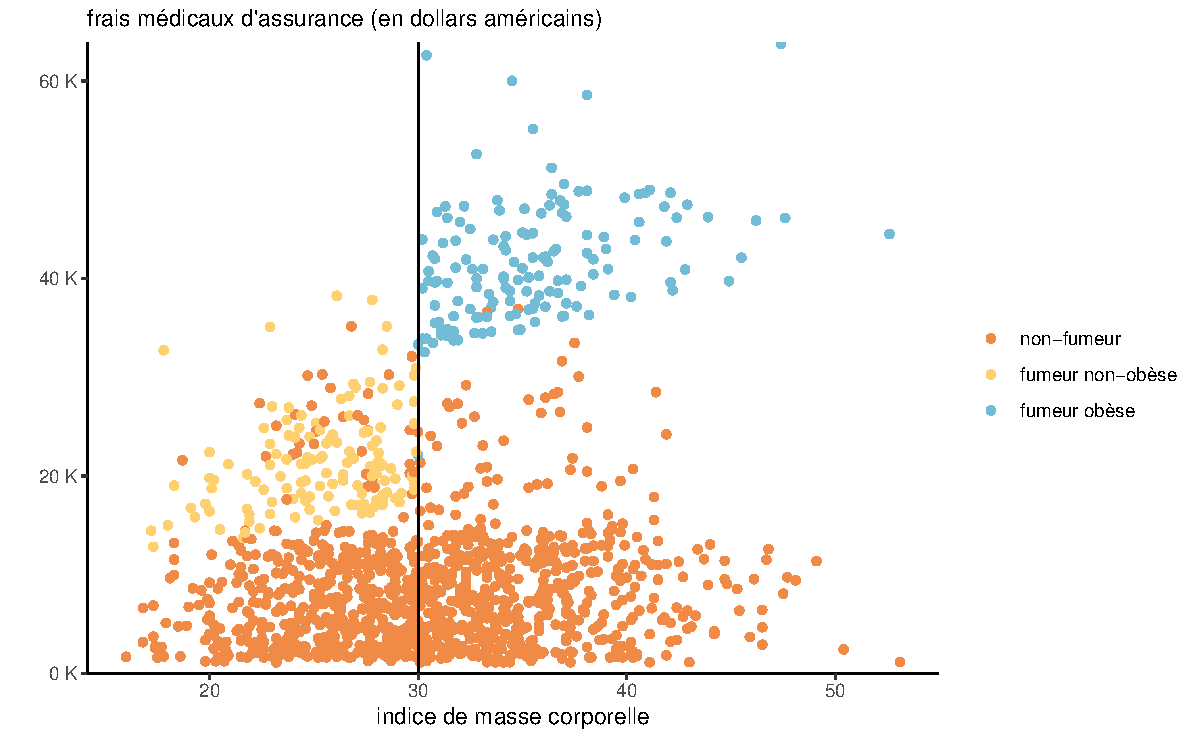
\includegraphics[width=0.85\textwidth,height=\textheight]{regression-lineaire_files/figure-pdf/fig-insuranceinter1-1.pdf}

}

\caption{\label{fig-insuranceinter1}Nuage de points des données
\texttt{assurance} avec les frais en fonction de l'\texttt{imc}, selon
le status \texttt{fumeur}.}

\end{figure}%

\end{example}

\begin{example}[Intention
d'achat]\protect\hypertarget{exm-intention}{}\label{exm-intention}

On considère un exemple avec des données bidons \texttt{interaction}. Le
modèle additif (sans interaction) a pour moyenne \begin{align*}
\mathsf{E}(\texttt{intention} \mid \cdot)=\beta_0 + \beta_1 \texttt{sexe} + \beta_2 \texttt{fixation},
\end{align*} où \(\texttt{sexe=1}\) pour les femmes et
\(\texttt{sexe=0}\) pour les hommes

L'effet de la variable continue \texttt{fixation} est identique pour les
deux sexes. De même, l'effet de la variable binaire est supposé être le
même pour toutes les valeurs possibles de la variable continue. Nous
pouvons le voir sur le graphique, car la différence entre les lignes
représente l'effet de \(\texttt{sexe}\), est le même pour toutes les
valeurs de \(\texttt{fixation}\); les lignes sont \emph{parallèles} :
voir le panneau gauche de Figure~\ref{fig-interaction-slope}.

\begin{figure}[ht!]

\centering{

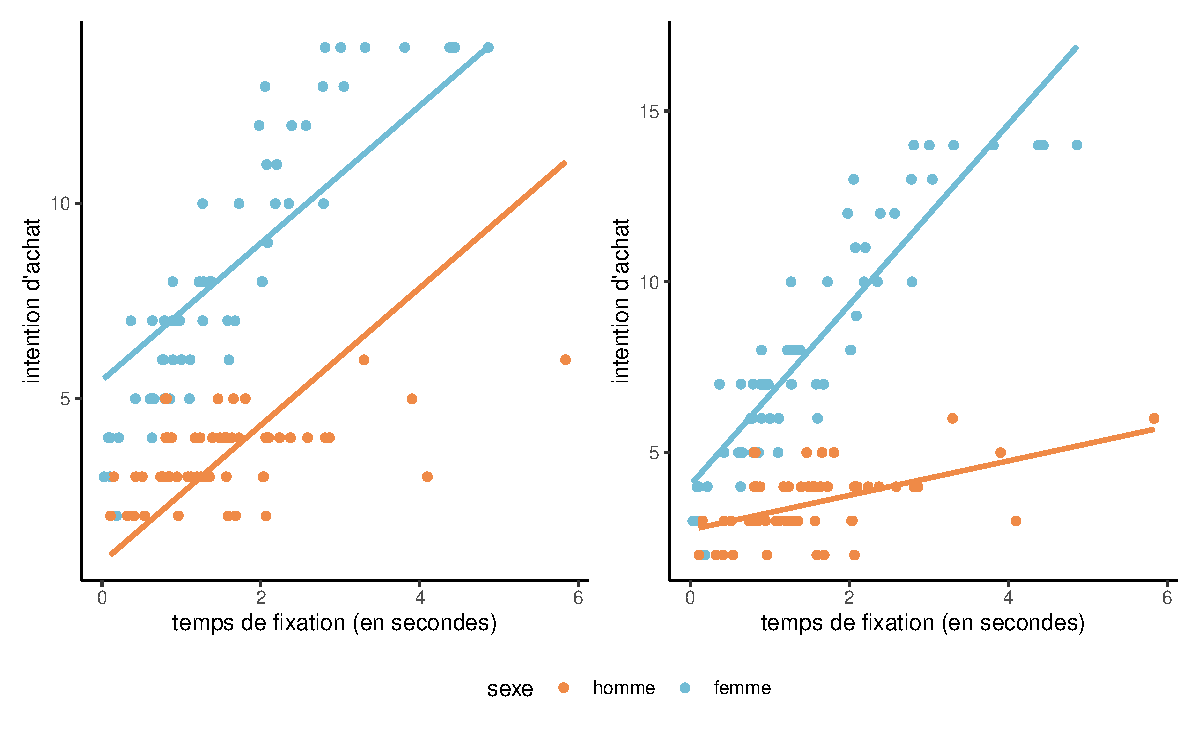
\includegraphics[width=0.85\textwidth,height=\textheight]{regression-lineaire_files/figure-pdf/fig-interaction-slope-1.pdf}

}

\caption{\label{fig-interaction-slope}Nuages de points et droites
ajustées pour un modèle sans interaction (gauche) et avec interaction
(droite).}

\end{figure}%

Pour ajuster une pente différente par sexe, on crée une nouvelle
variable égale au produit \(\texttt{fixation}\times\texttt{sexe}\) et on
l'ajoute à notre modèle, \begin{align*}
\mathsf{E}(\texttt{intention} \mid \cdot)= \beta_0 + \beta_1 \texttt{sexe} + \beta_2\texttt{fixation}  + \beta_3 \texttt{fixation}\cdot \texttt{sexe}.
\end{align*}

Selon la valeur de \(\texttt{sexe}\), on obtient \begin{align*}
\mathsf{E}(\texttt{intention} \mid \cdot) = 
\begin{cases}
(\beta_0 + \beta_1) + (\beta_2 + \beta_3)\texttt{fixation}, & \texttt{sexe}=1 \text{ (femme)},\\
  \beta_0 + \beta_2 \texttt{fixation}, & \texttt{sexe}=0 \text{ (homme)}.
\end{cases}
\end{align*} L'interprétation des coefficients du modèle se fait comme
d'habitude avec la paramétrisation (traitement):

\begin{itemize}
\tightlist
\item
  \(\beta_0\) est l'intention d'achat moyenne lorsque le temps de
  fixation est nul pour les hommes,
\item
  \(\beta_1\) est la différence d'ordonnée à l'origine entre les femmes
  et les hommes (différence d'intention d'achat moyenne entre femmes et
  hommes quand le temps de fixation est nul),
\item
  \(\beta_2\) est l'augmentation unitaire de l'intention d'achat par
  seconde de fixation pour les hommes,
\item
  \(\beta_3\) est la différence de pente entre les femmes et les hommes
  (différence d'intention d'achat moyenne femmes vs hommes pour une
  augmentation d'une seconde de fixation).
\end{itemize}

Tester la significativité de l'interaction revient à vérifier si
\(\mathscr{H}_0: \beta_3=0\).

\begin{Shaded}
\begin{Highlighting}[]
\FunctionTok{data}\NormalTok{(interaction, }\AttributeTok{package =} \StringTok{"hecmodstat"}\NormalTok{)}
\CommentTok{\# Pour spécifier une interaction, utiliser :}
\NormalTok{mod }\OtherTok{\textless{}{-}} \FunctionTok{lm}\NormalTok{(intention }\SpecialCharTok{\textasciitilde{}}\NormalTok{ sexe }\SpecialCharTok{+}\NormalTok{ fixation }\SpecialCharTok{+}\NormalTok{  sexe}\SpecialCharTok{:}\NormalTok{fixation, }
          \AttributeTok{data =}\NormalTok{ interaction)}
\CommentTok{\# Un raccourci est sexe*fixation, qui donne la même chose}
\FunctionTok{summary}\NormalTok{(mod)}\SpecialCharTok{$}\NormalTok{coefficients}
\CommentTok{\#\textgreater{}               Estimate Std. Error t value Pr(\textgreater{}|t|)}
\CommentTok{\#\textgreater{} (Intercept)      2.741      0.282    9.73 1.02e{-}16}
\CommentTok{\#\textgreater{} sexe             1.312      0.380    3.45 7.74e{-}04}
\CommentTok{\#\textgreater{} fixation         0.504      0.153    3.29 1.33e{-}03}
\CommentTok{\#\textgreater{} sexe:fixation    2.135      0.200   10.69 5.61e{-}19}
\end{Highlighting}
\end{Shaded}

Le modèle avec interaction est significativement meilleur, ce qui
signifie que l'effet du temps de fixation sur l'intention d'achat varie
en fonction du sexe.

\end{example}

\begin{refremark}[Principe de marginalité]
Tous les termes d'ordre inférieurs devraient être inclus si
l'interaction est présente.

Par exemple, on ne retirera pas \(\texttt{fixation}\) tout en conservant
le terme d'interaction \(\texttt{fixation*sexe}\), même si on ne rejette
pas \(\mathscr{H}_0:\beta_2=0\), puisqu'autrement \begin{align*}
&\mathsf{E}(\texttt{intention} \mid \cdot) =
\begin{cases}
(\beta_0 + \beta_1) + \beta_3\texttt{fixation}, & \texttt{sexe}=1 \text{ (femme)},\\
  \beta_0, &\texttt{sexe}=0 \text{ (homme)};                 
\end{cases}
\end{align*} cela implique que l'intention d'achat est constante pour
les hommes, quel que soit le temps de fixation.

Comme le choix de catégorie de référence est arbitraire, changer la
variable indicatrice \texttt{sexe} pour \(\texttt{0}\) pour les femmes,
\(\texttt{1}\) pour les hommes, donnerait un autre modèle et
potentiellement des inférences différentes. De ce fait, on ne considère
jamais le retrait d'un effet principal si la variable est incluse dans
une interaction. Le principe de \textbf{marginalité} suppose que tous
les termes d'ordre inférieurs devraient être inclus.

\label{rem-marginalite}

\end{refremark}

Le concept d'interaction se généralise à des variables catégorielles
avec plus de deux niveaux. Dans ce cas, on doit considérer la
statistique \(F\) pour l'ajout/l'élimination afin de vérifier la
significativité de l'interaction dans son ensemble.

\begin{definition}[Analyse de
variance]\protect\hypertarget{def-anova}{}\label{def-anova}

Une analyse de variance est un modèle linéaire dans lequel la moyenne
est une fonction de variables explicatives catégorielles. Si nous
disposons de données pour toutes les combinaisons différentes de
facteurs, les facteurs sont \textbf{croisés} et nous pouvons envisager
d'inclure leurs interactions.

\end{definition}

Considérons un modèle d'analyse de variance à deux facteurs, disons
\(A\) et \(B\), lesquels ont respectivement \(n_a\) et \(n_b\) niveaux.
Le modèle avec interaction s'écrit

\begin{equation}\phantomsection\label{eq-twowayasoneway}{
\underset{\text{réponse}\vphantom{b}}{Y_{ijk}} = \underset{\text{moyenne de sous-groupe}}{\mu_{ij}} + \underset{\text{aléa}}{\varepsilon_{ijk}}
}\end{equation} où

\begin{itemize}
\tightlist
\item
  \(Y_{ijk}\) est le \(k\)e mesure du \(i\)e niveau du facteur \(A\) et
  du \(j\)e niveau du facteur \(B\), disons \((a_i, b_j)\)
\item
  \(\mu_{ij}\) est la moyenne théorique du sous-groupe \((a_i, b_j)\)
\item
  \(\varepsilon_{ijk}\) sont des termes d'aléas indépendants de moyenne
  zéro et d'écart-type \(\sigma\).
\end{itemize}

Dans un devis factoriel complet avec interaction, on peut écrire
l'espérance de la variable réponse
\(\mathsf{E}(Y \mid A=a_i, B=b_j) = \mu_{ij}\). Ce modèle peut être vu
comme une analyse de variance à un facteur doté de \(n_an_b\) niveaux.
Cette observation peut être utile pour spécifier les poids de contrastes
linéaires ou lorsqu'il existe un groupe de contrôle supplémentaire dans
un cadre expérimental. Toutefois, la structure permet de spécifier les
hypothèses d'intérêt.

Nous pouvons l'exprimer de manière équivalente en termes d'ordonnée à
l'origine, d'effets principaux de l'une ou l'autre variable et de termes
d'interaction. Le modèle additif, sans interaction, a une moyenne pour
la cellule \((i,j)\) de

\begin{align*}
\mathsf{E}(Y_{ij} \mid A = a_i, B=b_j) = \mu + \alpha_i + \beta_j.
\end{align*}

Nous pouvons envisager des simplifications de modèle de bas en haut. La
suppression de l'interaction conduit à un modèle avec
\(1 + (n_a-1) + (n_b-1)\) paramètres, par rapport à \(n_a \times n_b\)
pour le modèle avec l'interaction. Nous pouvons utiliser un test \(F\)
pour vérifier la significativité de ce dernier. Si les facteurs
n'interagissent pas, la moyenne dans la cellule est donnée par la somme
des effets principaux. Ce n'est qu'après avoir supprimé ce terme que
nous pouvons déterminer si toutes les moyennes des lignes ou des
colonnes sont identiques.

:::

Bien que des tests formels soient nécessaires pour vérifier les
interactions, le concept peut être mieux compris en examinant des
graphiques.

\begin{definition}[Diagramme
d'interaction]\protect\hypertarget{def-interactionplot}{}\label{def-interactionplot}

Nous pouvons essayer de détecter visuellement les interactions en
traçant la réponse (moyenne) en fonction de l'une des covariables, en
utilisant ce que l'on appelle un \textbf{diagramme d'interaction}.
Lorsqu'il y a plus de deux variables catégorielles, nous pouvons
utiliser des couleurs, des symboles ou des panneaux pour représenter les
catégories. L'absence d'interaction dans ces diagrammes implique des
lignes parallèles, mais il faut tenir compte de l'incertitude.

\begin{figure}[ht!]

\centering{

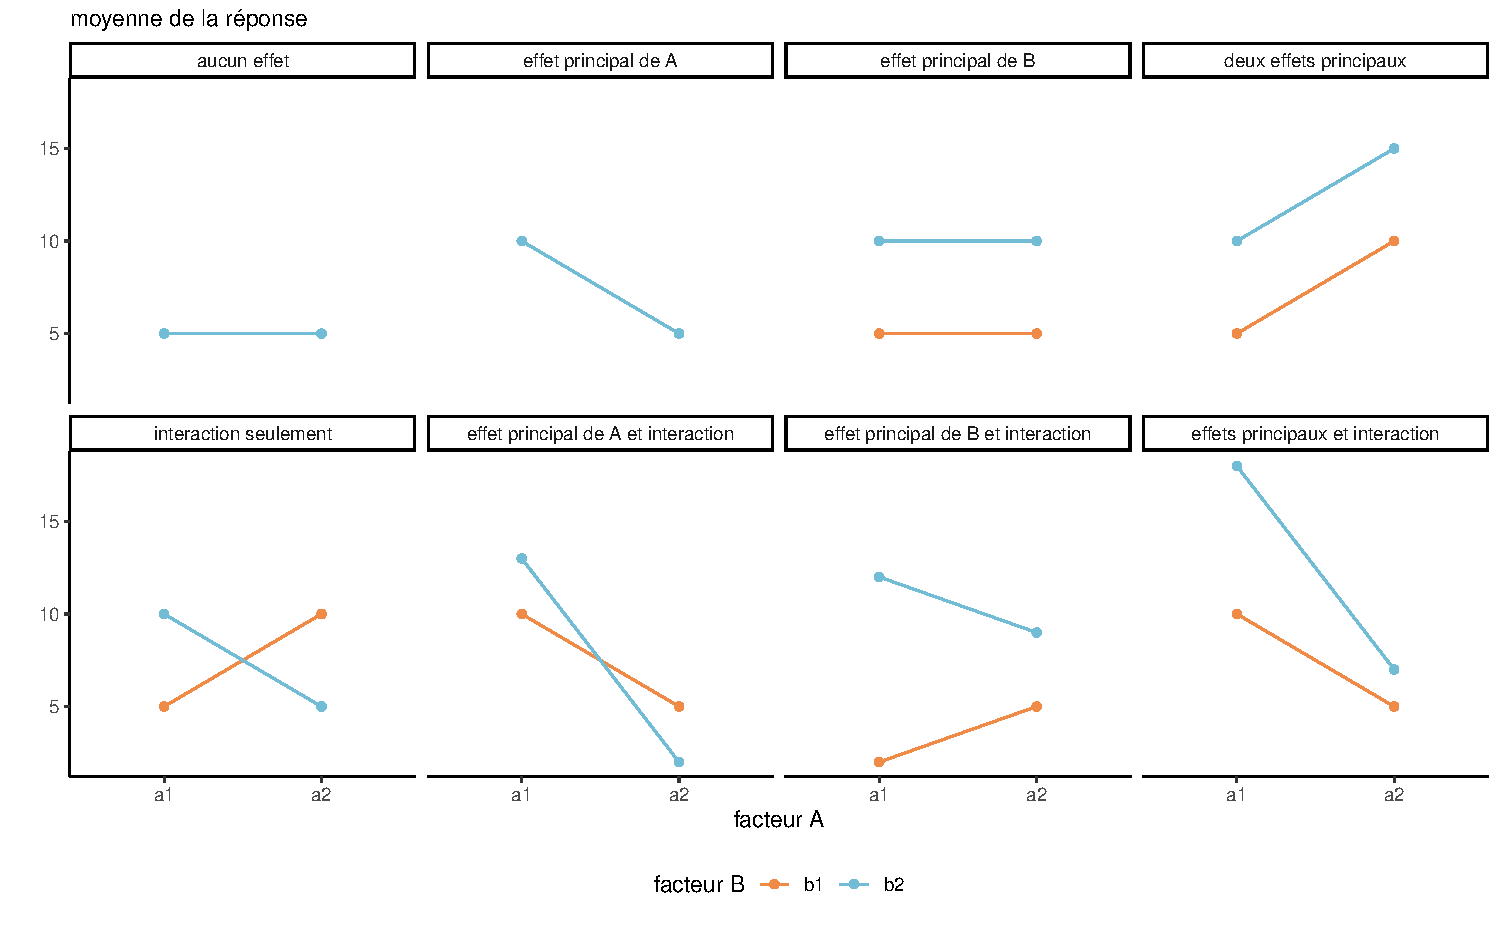
\includegraphics[width=1\textwidth,height=\textheight]{regression-lineaire_files/figure-pdf/fig-2by2-1.pdf}

}

\caption{\label{fig-2by2}Diagramme d'interactions pour un devis 2 par 2.
Image adaptée de la Figure 10.2 de Crump, Navarro, et Suzuki
(\citeproc{ref-Crump.Navarro.Suzuki:2019}{2019}) par Matthew Crump
(licence CC BY-SA 4.0).}

\end{figure}%

\end{definition}

\begin{definition}[Effets simples et effets
principaux]\protect\hypertarget{def-simple}{}\label{def-simple}

Lorsqu'il n'y a pas d'interactions, il est logique de faire abstraction
d'une ou plusieurs variables et de considérer les \textbf{effets
marginaux}, obtenus en regroupant les données des facteurs omis, en
calculant la moyenne équipondérée des sous-groupes. Supposons, par
exemple, que nous soyons intéressés par la comparaison des niveaux de
\(A\). Lorsque les interactions entre \(A\) et \(B\) ne sont pas
significatives, nous pouvons considérer des termes d'ordre inférieur et
rapporter les \textbf{moyennes marginales estimées} et les contrastes
entre les moyennes de \(A\). Si l'interaction avec \(B\) a un impact,
nous pouvons plutôt calculer la moyenne de la sous-cellule
\(A \mid B=b_j\), et de la même manière pour les contrastes. Nous
distinguons donc les cas suivants :

\begin{itemize}
\tightlist
\item
  \textbf{effets simples}: différences entre les niveaux d'un élément
  dans une combinaison fixe d'autres éléments. Les effets simples
  consistent à comparer les moyennes des cellules dans une ligne ou une
  colonne donnée.
\item
  \textbf{effets principaux} : différences par rapport à la moyenne pour
  chaque condition d'un facteur. Les effets principaux sont des moyennes
  de lignes ou de colonnes.
\end{itemize}

\end{definition}

\begin{example}[Effet psychologique
d'emprunt]\protect\hypertarget{exm-STC21-twoway}{}\label{exm-STC21-twoway}

L'étude complémentaire 5 de Sharma, Tully, et Cryder
(\citeproc{ref-Sharma.Tully.Cryder:2021}{2021}) vérifie la perception
psychologique de l'emprunt en fonction du terme employé pour désigner le
montant monétaire. Les auteurs ont effectué une comparaison deux par
deux inter-sujets (ANOVA à deux facteurs) en faisant varier le type de
dette (si l'argent était proposé sous forme de crédit (\texttt{credit})
ou prêt (\texttt{loan}), de même que le type d'achat pour lequel
l'argent serait utilisé, soit dépenses discrétionnaires
(\texttt{discretionary}) ou pour combler à des besoins essentiels
(\texttt{need}). La réponse est la moyenne de (a) la probabilité et de
(b) l'intérêt pour le produit, toutes deux mesurés à l'aide d'une
échelle de Likert allant de 1 à 9.

Le modèle pour la moyenne avec interaction peut être écrit en utilisant
la paramétrisation usuelle comme suit \begin{align*}
\texttt{likelihood} &= \beta_0 + \beta_1\mathbf{1}_{\texttt{purchase=need}} + \beta_2\mathbf{1}_{\texttt{debttype=loan}} \\&\quad+ \beta_3\mathbf{1}_{\texttt{purchase=need}}\mathbf{1}_{\texttt{debttype=loan}} + \varepsilon
\end{align*}

On peut calculer la moyenne de chaque groupe et déduire l'interprétation
des coefficients:

\begin{itemize}
\tightlist
\item
  \(\mu_1 = \beta_0\) pour \texttt{purchase=discretionnary} et
  \texttt{debttype=credit}
\item
  \(\mu_2 = \beta_0 + \beta_1\) pour \texttt{purchase=need} et
  \texttt{debttype=credit}
\item
  \(\mu_1 = \beta_0 + \beta_2\) pour \texttt{purchase=discretionnary} et
  \texttt{debttype=loan}
\item
  \(\mu_2 = \beta_0 + \beta_1 + \beta_2 + \beta_3\) pour
  \texttt{purchase=need} et \texttt{debttype=loan}
\end{itemize}

Ainsi, \(\beta_3\) représente la différence des moyennes
\(\mu_1 + \mu_4 - \mu_2 - \mu_3\).

Sharma, Tully, et Cryder (\citeproc{ref-Sharma.Tully.Cryder:2021}{2021})
a ajusté un modèle avec deux facteurs, chacun avec deux niveaux, et leur
interaction. Comme il y a une moyenne globale et deux effets principaux
(différence supplémentaire de moyenne pour les deux facteurs
\texttt{debttype} et \texttt{purchase}), l'interaction a un degré de
liberté puisque nous passons d'un modèle avec trois paramètres à un
modèle qui a une moyenne différente pour chacun des quatre sous-groupes.

La raison pour laquelle on teste d'abord la présence d'interaction est
que, si l'effet d'un facteur dépend du niveau de l'autre, comme le
montre Figure~\ref{fig-2by2}, il faut alors comparer l'étiquette du type
de dette séparément pour chaque type d'achat et vice-versa à l'aide
d'effets simples. Si l'interaction n'est pas significative, nous pouvons
regrouper les observations pour obtenir une ANOVA à un facteur, ce qui
donne les comparaisons marginales avec les effets principaux.

L'ajustement du modèle incluant l'interaction entre les facteurs
garantit que nous conservons l'hypothèse d'additivité et que nos
conclusions ne sont pas trompeuses: le prix à payer est l'estimation de
paramètres moyens supplémentaires, ce qui n'est pas un problème si vous
recueillez suffisamment de données, mais peut être critique lorsque la
collecte de données est extrêmement coûteuse et que seules quelques
observations sont disponibles pour chaque sous-groupe.

Dans \textbf{R}, on inclut les deux facteurs et leurs interactions avec
\texttt{reponse\ \textasciitilde{}\ facteurA\ *\ facteurB}, le symbole
\texttt{*} indiquant que les deux interagissent, un raccourci pour
\texttt{facteuA\ +\ facteurB\ +\ facteurA:facteurB}; dans un modèle avec
seulement les effets principaux, on sépare les facteurs par un
\texttt{+} pour obtenir le modèle additif.

\begin{Shaded}
\begin{Highlighting}[]
\CommentTok{\# Données de l\textquotesingle{}étude supp. 5}
\CommentTok{\# de Sharma, Tully, et Cryder (2021)}
\FunctionTok{data}\NormalTok{(STC21\_SS5, }\AttributeTok{package =} \StringTok{"hecedsm"}\NormalTok{)}
\CommentTok{\# La fonction \textquotesingle{}aov\textquotesingle{} sert à ajuste des ANOVA}
\CommentTok{\# Équivalent à "lm" avec variables catégorielles, contrasts somme nulle}
\NormalTok{modlin\_STC21 }\OtherTok{\textless{}{-}} \FunctionTok{aov}\NormalTok{(}
\NormalTok{    likelihood }\SpecialCharTok{\textasciitilde{}}\NormalTok{ purchase}\SpecialCharTok{*}\NormalTok{debttype, }
    \AttributeTok{data =}\NormalTok{ STC21\_SS5)}
\CommentTok{\# Calculer le décompte par sous{-}catégorie (données débalancées)}
\FunctionTok{xtabs}\NormalTok{(}\SpecialCharTok{\textasciitilde{}}\NormalTok{ purchase }\SpecialCharTok{+}\NormalTok{ debttype, }\AttributeTok{data =}\NormalTok{ STC21\_SS5)}
\CommentTok{\#\textgreater{}                debttype}
\CommentTok{\#\textgreater{} purchase        credit loan}
\CommentTok{\#\textgreater{}   discretionary    392  359}
\CommentTok{\#\textgreater{}   need             361  389}
\CommentTok{\# Calcul de la moyenne globale/lignes/colonnes/cellules}
\NormalTok{moy\_groupes }\OtherTok{\textless{}{-}} \FunctionTok{model.tables}\NormalTok{(modlin\_STC21, }\AttributeTok{type =} \StringTok{"means"}\NormalTok{)}

\CommentTok{\# Tableau d\textquotesingle{}ANOVA avec effets de type 2}
\NormalTok{car}\SpecialCharTok{::}\FunctionTok{Anova}\NormalTok{(modlin\_STC21, }\AttributeTok{type =} \DecValTok{2}\NormalTok{)}
\CommentTok{\#\textgreater{} Anova Table (Type II tests)}
\CommentTok{\#\textgreater{} }
\CommentTok{\#\textgreater{} Response: likelihood}
\CommentTok{\#\textgreater{}                   Sum Sq   Df F value  Pr(\textgreater{}F)    }
\CommentTok{\#\textgreater{} purchase             752    1   98.21 \textless{} 2e{-}16 ***}
\CommentTok{\#\textgreater{} debttype              92    1   12.04 0.00054 ***}
\CommentTok{\#\textgreater{} purchase:debttype     14    1    1.79 0.18171    }
\CommentTok{\#\textgreater{} Residuals          11467 1497                    }
\CommentTok{\#\textgreater{} {-}{-}{-}}
\CommentTok{\#\textgreater{} Signif. codes:  0 \textquotesingle{}***\textquotesingle{} 0.001 \textquotesingle{}**\textquotesingle{} 0.01 \textquotesingle{}*\textquotesingle{} 0.05 \textquotesingle{}.\textquotesingle{} 0.1 \textquotesingle{} \textquotesingle{} 1}
\end{Highlighting}
\end{Shaded}

L'interaction n'étant pas significative, nous pouvons n'interpréter que
l'effet principal de la fixation.

Cette différence de moyenne conditionnelle est appelée effet marginal,
car elle est obtenue en calculant la moyenne de toutes les
sous-catégories pour un même niveau du facteur. Le modèle estime
cependant la variance sur la base des résidus du modèle d'interaction
complet avec quatre moyennes de cellules, et diffère donc de celui
obtenu en exécutant (à tort) un modèle avec seulement \texttt{purchase}
comme variable explicative.

Dans le tableau d'analyse de la variance, nous nous concentrons
exclusivement sur la dernière ligne avec la somme des carrés pour
l'interaction \texttt{purchase:debttype}. La statistique \(F\) est 1.79;
avec la loi de référence \(\mathsf{Fisher}\) (1, 1497), on obtient une
valeur-\(p\) de 0.18 alors il n'y a pas de preuve que l'effet du libellé
pour l'achat dépende du type de dette.

On peut donc regrouper les données et étudier uniquement l'effet du
libellé (prêt \texttt{loan} ou \texttt{credit}) en combinant les données
pour les types d'achats, une des comparaisons planifiées des annexes en
ligne. Pour ce faire, on utilise la fonction \texttt{emmeans} du paquet
éponyme en spécifiant le nom du ou des facteurs d'intérêts (ceux que
l'on veut conserver) avec l'argument \texttt{specs}. Par défaut, on
calcule les moyennes marginales estimées, l'argument
\texttt{contr\ =\ "pairwise"} indique que l'on veut en plus les
différences deux à deux, ici le seul contraste possible pour des
différences entre deux facteurs.

\begin{Shaded}
\begin{Highlighting}[]
\CommentTok{\# Comparisons deux à deux au sein des niveaux de "purchase"}
\CommentTok{\# Effets simples}
\NormalTok{emmeans}\SpecialCharTok{::}\FunctionTok{emmeans}\NormalTok{(modlin\_STC21, }
                 \AttributeTok{specs =} \StringTok{"purchase"}\NormalTok{,}
                 \AttributeTok{contr =} \StringTok{"pairwise"}\NormalTok{)}
\CommentTok{\#\textgreater{} $emmeans}
\CommentTok{\#\textgreater{}  purchase      emmean    SE   df lower.CL upper.CL}
\CommentTok{\#\textgreater{}  discretionary   4.17 0.101 1497     3.97     4.36}
\CommentTok{\#\textgreater{}  need            5.58 0.101 1497     5.39     5.78}
\CommentTok{\#\textgreater{} }
\CommentTok{\#\textgreater{} Results are averaged over the levels of: debttype }
\CommentTok{\#\textgreater{} Confidence level used: 0.95 }
\CommentTok{\#\textgreater{} }
\CommentTok{\#\textgreater{} $contrasts}
\CommentTok{\#\textgreater{}  contrast             estimate    SE   df t.ratio p.value}
\CommentTok{\#\textgreater{}  discretionary {-} need    {-}1.42 0.143 1497  {-}9.910  \textless{}.0001}
\CommentTok{\#\textgreater{} }
\CommentTok{\#\textgreater{} Results are averaged over the levels of: debttype}
\CommentTok{\# Diagramme d\textquotesingle{}interaction}
\NormalTok{emmeans}\SpecialCharTok{::}\FunctionTok{emmip}\NormalTok{(modlin\_STC21, }
\NormalTok{               purchase }\SpecialCharTok{\textasciitilde{}}\NormalTok{ debttype, }
               \AttributeTok{CIs =} \ConstantTok{TRUE}\NormalTok{) }\SpecialCharTok{+}
  \FunctionTok{theme\_minimal}\NormalTok{()}
\end{Highlighting}
\end{Shaded}

\begin{figure}[ht!]

\centering{

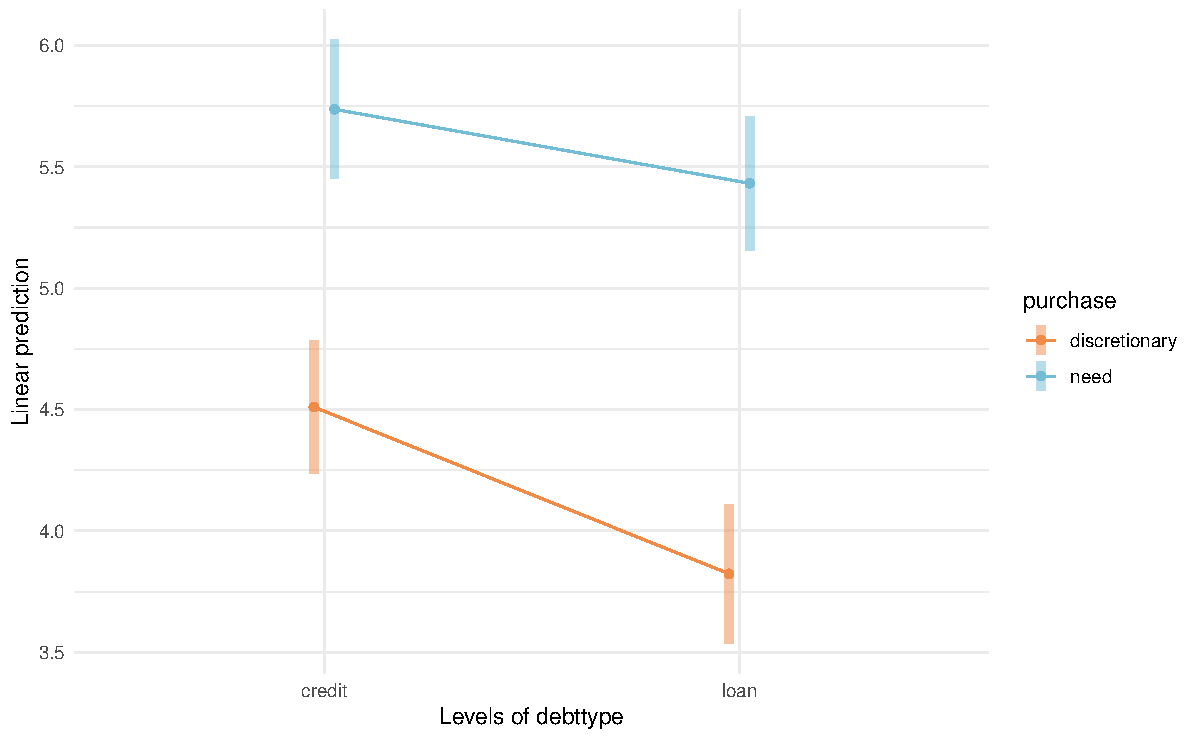
\includegraphics[width=0.85\textwidth,height=\textheight]{regression-lineaire_files/figure-pdf/fig-interaction-ST-1.pdf}

}

\caption{\label{fig-interaction-ST}Diagramme d'interaction pour les
données de l'étude S5 de Sharma, Tully, et Cryder
(\citeproc{ref-Sharma.Tully.Cryder:2021}{2021}).}

\end{figure}%

\end{example}

\begin{refremark}[Décomposition de sommes des carrés]
Il existe différentes décompositions de la somme des carrés (type I, II
et III) pour la comparaison des modèles emboîtés dans les tableaux
d'analyse de la variance.

Ces décompositions testent différents modèles à l'aide des statistiques
\(F\), avec le même dénominateur basé sur l'estimation de l'écart-type,
mesuré avec \(S_2\), de la sortie du modèle complet. Le numérateur est
la différence dans la somme des carrés. Toutes les décompositions
concordent lorsque le plan d'expérience est \textbf{équilibré}, ce qui
signifie que chaque cellule a le même nombre de réplications \(n_r\), de
sorte que le nombre total d'observations est \(n = n_an_bn_r\).

\begin{longtable}[]{@{}
  >{\raggedright\arraybackslash}p{(\columnwidth - 6\tabcolsep) * \real{0.2065}}
  >{\raggedright\arraybackslash}p{(\columnwidth - 6\tabcolsep) * \real{0.2500}}
  >{\raggedright\arraybackslash}p{(\columnwidth - 6\tabcolsep) * \real{0.2500}}
  >{\raggedright\arraybackslash}p{(\columnwidth - 6\tabcolsep) * \real{0.2935}}@{}}

\caption{\label{tbl-ssdecompo}Décomposition de la somme des carrés dans
les tableaux d'ANOVA (termes de l'hypothèse nulle vs l'alternative).}

\tabularnewline

\toprule\noalign{}
\begin{minipage}[b]{\linewidth}\raggedright
\end{minipage} & \begin{minipage}[b]{\linewidth}\raggedright
type I
\end{minipage} & \begin{minipage}[b]{\linewidth}\raggedright
type II
\end{minipage} & \begin{minipage}[b]{\linewidth}\raggedright
type III
\end{minipage} \\
\midrule\noalign{}
\endhead
\bottomrule\noalign{}
\endlastfoot
\(\boldsymbol{A}\) & intercept vs \(A\) & \(B\) vs \((A,B)\) &
\((B, A:B)\) vs \((A,B, A:B)\) \\
\(\boldsymbol{B}\) & \(A\) vs \((A,B)\) & \(A\) vs \((A,B)\) &
\((A, A:B)\) vs \((A,B,A:B)\) \\
\(\boldsymbol{A:B}\) & \((A,B)\) vs \((A,B,A:B)\) & \((A,B)\) vs
\((A,B,A:B)\) & \((A,B)\) vs \((A,B,A:B)\) \\

\end{longtable}

Tableau~\ref{tbl-ssdecompo} montre les différentes sommes des erreurs
quadratiques des modèles, avec les termes entre parenthèses indiquant
quels termes sont inclus (\(A:B\) désigne l'interaction).

La décomposition de type I, la valeur par défaut du générique
\texttt{anova}, utilise l'ordre dans lequel les termes sont spécifiés,
disons \(A\), \(B\), \(AB\), et compare donc sur la première ligne
l'amélioration dans le modèle de la moyenne seule avec \(A\), puis sur
la deuxième ligne le test pour \(B\) compare le modèle avec les deux
effets principaux \(A\) et \(B\) avec seulement \(A\). Étant donné que
l'ordre dans lequel les facteurs sont spécifiés est arbitraire, cette
décomposition est arbitraire et donc non pertinente.

La décomposition de type II considère les termes de même niveau dans la
hiérarchie, de sorte que les tests pour les effets principaux sont
\(A + B\) vs \(A\), \(A+B\) vs \(B\) et celui de l'interaction est
\(A\times B\) vs \(A, B\). Il s'agit de l'option par défaut si l'on
souhaite considérer les effets principaux lorsque l'interaction n'est
pas significative.

La décomposition de type III, popularisée par SAS et souvent choisie par
défaut dans les logiciels, prend en compte tous les autres termes, et
testerait donc les effets principaux comme \(A + B + A\times B\) vs
\(B + A\times B\). Cette méthode ne respecte pas le principe de
marginalité et doit donc être évitée. Les tests pour \(A\) ou \(B\) ne
doivent pas être utilisés.

Les trois méthodes donnent le même résultat et la même comparaison pour
le dernier niveau avec l'interaction.

\label{rem-sumofsquare}

\end{refremark}

Toutes les discussions relatives à une ANOVA à deux voies s'appliquent à
des plans d'expérience à \(K\) facteurs. Cependant, le fléau de la
dimensionnalité rend plus difficile la collecte d'observations dans
chaque cellule. Toute ANOVA à plusieurs facteurs peut être ramenée à une
ANOVA à un facteur: ceci est particulièrement utile lorsqu'il y a un
groupe de contrôle qui n'est pas lié aux niveaux des facteurs, étant
donné qu'il n'y a pas de manipulation. L'utilisation des contrastes
devient critique puisque nous pouvons écrire n'importe quel test pour
les effets principaux, les interactions, etc.

\begin{example}[Perception d'appropriation culturelle par idéologie
politique]\protect\hypertarget{exm-LKUK24}{}\label{exm-LKUK24}

On considère un modèle d'ANOVA à trois facteurs de Lin et al.
(\citeproc{ref-Lin.Kim.Uduehi.Keinan:2024}{2024}). Leur étude 4
s'intéresse à l'appropriation culturelle pour une recette de \emph{soul
food}, un courant afro-américain, parue dans le livre du ``Chef Dax''.
Les auteurs manipulent l'ethnicité du chef, afro-Américain ou pas, et la
façon dont la recette a été obtenue (furtivement, en demandant la
permission ou sans mention dans le cas du groupe contrôle). Les auteurs
ont postulé que la perception de l'appropriation varie selon l'idéologie
politique. L'étude utilise un devis expérimental
\(3 \times 2 \times 2\).

\begin{Shaded}
\begin{Highlighting}[]
\FunctionTok{data}\NormalTok{(LKUK24\_S4, }\AttributeTok{package =} \StringTok{"hecedsm"}\NormalTok{)}
\CommentTok{\# Vérifier la répartition d\textquotesingle{}observations en sous{-}groupes}
\FunctionTok{xtabs}\NormalTok{(}\SpecialCharTok{\textasciitilde{}}\NormalTok{politideo }\SpecialCharTok{+}\NormalTok{ chefdax }\SpecialCharTok{+}\NormalTok{ brandaction,}
          \AttributeTok{data =}\NormalTok{ LKUK24\_S4)}
\CommentTok{\#\textgreater{} , , brandaction = peeking}
\CommentTok{\#\textgreater{} }
\CommentTok{\#\textgreater{}               chefdax}
\CommentTok{\#\textgreater{} politideo      not black black}
\CommentTok{\#\textgreater{}   conservative        33    36}
\CommentTok{\#\textgreater{}   liberal             87    84}
\CommentTok{\#\textgreater{} }
\CommentTok{\#\textgreater{} , , brandaction = permission}
\CommentTok{\#\textgreater{} }
\CommentTok{\#\textgreater{}               chefdax}
\CommentTok{\#\textgreater{} politideo      not black black}
\CommentTok{\#\textgreater{}   conservative        42    34}
\CommentTok{\#\textgreater{}   liberal             77    84}
\CommentTok{\#\textgreater{} }
\CommentTok{\#\textgreater{} , , brandaction = control}
\CommentTok{\#\textgreater{} }
\CommentTok{\#\textgreater{}               chefdax}
\CommentTok{\#\textgreater{} politideo      not black black}
\CommentTok{\#\textgreater{}   conservative        38    32}
\CommentTok{\#\textgreater{}   liberal             79    85}
\CommentTok{\# Les facteurs sont croisés et il y a des réplications}
\CommentTok{\# On ajuste un modèle d\textquotesingle{}ANOVA à trois facteurs (avec toutes les interactions)}
\NormalTok{mod }\OtherTok{\textless{}{-}} \FunctionTok{lm}\NormalTok{(appropriation }\SpecialCharTok{\textasciitilde{}}\NormalTok{ politideo }\SpecialCharTok{*}\NormalTok{ chefdax }\SpecialCharTok{*}\NormalTok{ brandaction,}
          \AttributeTok{data =}\NormalTok{ LKUK24\_S4)}
\CommentTok{\# Calculer les estimations des moyennes marginales }
\CommentTok{\# pour chacun des 12 sous{-}groupes}
\NormalTok{emm }\OtherTok{\textless{}{-}} \FunctionTok{emmeans}\NormalTok{(mod, }
        \AttributeTok{specs =} \FunctionTok{c}\NormalTok{(}\StringTok{"chefdax"}\NormalTok{, }\StringTok{"brandaction"}\NormalTok{, }\StringTok{"politideo"}\NormalTok{))}
\CommentTok{\# Créer un diagramme d\textquotesingle{}interaction}
\FunctionTok{emmip}\NormalTok{(}\AttributeTok{object =}\NormalTok{ emm, }
        \AttributeTok{formula =}\NormalTok{ brandaction }\SpecialCharTok{\textasciitilde{}}\NormalTok{ chefdax }\SpecialCharTok{|}\NormalTok{ politideo, }
        \AttributeTok{CIs =} \ConstantTok{TRUE}\NormalTok{) }\SpecialCharTok{+}
\FunctionTok{labs}\NormalTok{(}\AttributeTok{y =} \StringTok{"prédicteur linéaire"}\NormalTok{,}
     \AttributeTok{x =} \StringTok{"niveaux de chefdax"}\NormalTok{)}
\CommentTok{\# Tableau d\textquotesingle{}ANOVA (type 2)}
\NormalTok{anova\_tab }\OtherTok{\textless{}{-}}\NormalTok{ car}\SpecialCharTok{::}\FunctionTok{Anova}\NormalTok{(mod, }\AttributeTok{type =} \DecValTok{2}\NormalTok{)}
\end{Highlighting}
\end{Shaded}

\begin{center}
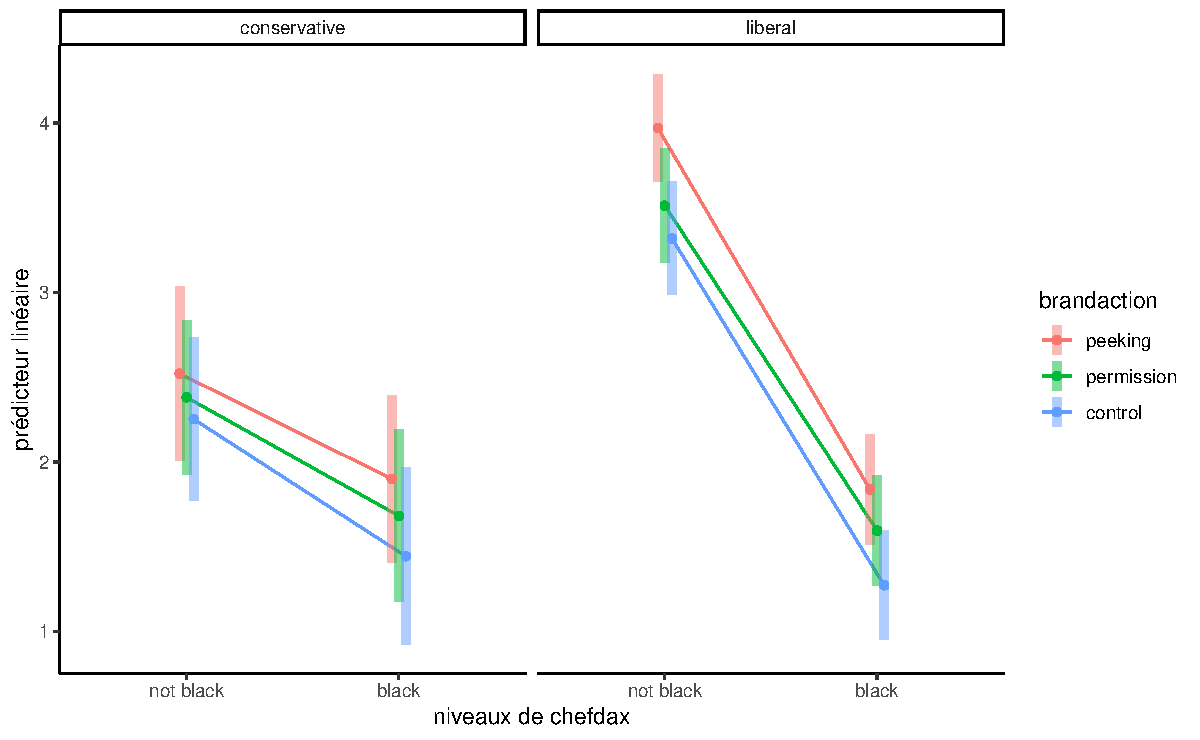
\includegraphics[width=0.85\textwidth,height=\textheight]{regression-lineaire_files/figure-pdf/unnamed-chunk-39-1.pdf}
\end{center}

Pour l'ANOVA à \(K\) facteurs, nous commençons toujours par estimer le
modèle complet avec toutes les interactions (à condition qu'il y ait
suffisamment de données pour estimer ces dernières, ce qui implique
qu'il y ait des répétitions). Si cette dernière est significative, nous
pouvons fixer un ou plusieurs niveaux de facteurs et comparer les
autres.

\begin{longtable}[]{@{}
  >{\raggedright\arraybackslash}p{(\columnwidth - 8\tabcolsep) * \real{0.4478}}
  >{\raggedleft\arraybackslash}p{(\columnwidth - 8\tabcolsep) * \real{0.2537}}
  >{\raggedleft\arraybackslash}p{(\columnwidth - 8\tabcolsep) * \real{0.0597}}
  >{\raggedleft\arraybackslash}p{(\columnwidth - 8\tabcolsep) * \real{0.1045}}
  >{\raggedright\arraybackslash}p{(\columnwidth - 8\tabcolsep) * \real{0.1343}}@{}}

\caption{\label{tbl-anova-LKUK24}Tableau d'analyse de variance
(décomposition de type 2) pour l'étude 4 de Lin et al.
(\citeproc{ref-Lin.Kim.Uduehi.Keinan:2024}{2024}).}

\tabularnewline

\toprule\noalign{}
\begin{minipage}[b]{\linewidth}\raggedright
terme
\end{minipage} & \begin{minipage}[b]{\linewidth}\raggedleft
somme des carrés
\end{minipage} & \begin{minipage}[b]{\linewidth}\raggedleft
ddl
\end{minipage} & \begin{minipage}[b]{\linewidth}\raggedleft
stat
\end{minipage} & \begin{minipage}[b]{\linewidth}\raggedright
valeur-p
\end{minipage} \\
\midrule\noalign{}
\endhead
\bottomrule\noalign{}
\endlastfoot
politideo & 48.49 & 1 & 21.35 & \textless0.001 \\
chefdax & 473.72 & 1 & 208.61 & \textless0.001 \\
brandaction & 34.24 & 2 & 7.54 & \textless0.001 \\
politideo:chefdax & 65.00 & 1 & 28.63 & \textless0.001 \\
politideo:brandaction & 1.56 & 2 & 0.34 & 0.71 \\
chefdax:brandaction & 0.62 & 2 & 0.14 & 0.87 \\
politideo:chefdax:brandaction & 0.66 & 2 & 0.15 & 0.86 \\
Residuals & 1587.33 & 699 & & \\

\end{longtable}

Si on considère le Tableau~\ref{tbl-anova-LKUK24}, nous constatons qu'il
n'y a pas d'interaction à trois voies et, si l'on omet cette dernière et
que l'on se concentre sur les niveaux inférieurs, une seule interaction
à deux voies entre l'idéologie politique et la race du chef Dax.Nous ne
pouvons pas interpréter la valeur \(p\) pour l'effet principal de
\texttt{brandaction}, mais nous pouvons examiner les moyennes
marginales.

Sur la base des données, nous réduirons les données à une ANOVA à une
voie comparant les trois niveaux de \texttt{brandaction} et à une ANOVA
à deux facteurs, \(2 \times 2\) pour \texttt{chefdax} et
\texttt{politideo}. Les résultats sont obtenus en calculant la moyenne
pour le facteur manquant, mais en estimant l'écart-type du modèle
complet.

Nous souhaitons comparer la perception de la race du chef Dax (noir ou
non), car la cuisine \emph{soul} est plus susceptible d'être associée à
l'appropriation culturelle si le chef Dax n'est pas noir. Nous procédons
avec \texttt{emmeans} en calculant les moyennes marginales séparément
pour chacune des quatre sous-catégories, mais nous comparons la race du
chef Dax séparément pour les libéraux et les conservateurs en raison de
la présence de l'interaction.

\begin{Shaded}
\begin{Highlighting}[]
\FunctionTok{data}\NormalTok{(LKUK24\_S4, }\AttributeTok{package =} \StringTok{"hecedsm"}\NormalTok{)}
\FunctionTok{library}\NormalTok{(emmeans)}
\NormalTok{mod }\OtherTok{\textless{}{-}} \FunctionTok{lm}\NormalTok{(appropriation }\SpecialCharTok{\textasciitilde{}}\NormalTok{ politideo }\SpecialCharTok{*}\NormalTok{ chefdax }\SpecialCharTok{*}\NormalTok{ brandaction,}
   \AttributeTok{data =}\NormalTok{ LKUK24\_S4)}
\CommentTok{\# Moyennes marginales pour }
\CommentTok{\# idéologie politique/ethnicité du Chef Dax}
\CommentTok{\# Calculer les effets simples séparément}
\CommentTok{\#  pour chaque idéologie politique}
\FunctionTok{emmeans}\NormalTok{(mod, }
         \AttributeTok{specs =} \StringTok{"chefdax"}\NormalTok{, }
         \AttributeTok{by =} \StringTok{"politideo"}\NormalTok{,}
         \AttributeTok{contrast =} \StringTok{"pairwise"}\NormalTok{)}
\CommentTok{\#\textgreater{} politideo = conservative:}
\CommentTok{\#\textgreater{}  chefdax   emmean     SE  df lower.CL upper.CL}
\CommentTok{\#\textgreater{}  not black   2.38 0.1425 699     2.11     2.66}
\CommentTok{\#\textgreater{}  black       1.68 0.1494 699     1.38     1.97}
\CommentTok{\#\textgreater{} }
\CommentTok{\#\textgreater{} politideo = liberal:}
\CommentTok{\#\textgreater{}  chefdax   emmean     SE  df lower.CL upper.CL}
\CommentTok{\#\textgreater{}  not black   3.60 0.0968 699     3.41     3.79}
\CommentTok{\#\textgreater{}  black       1.57 0.0947 699     1.38     1.75}
\CommentTok{\#\textgreater{} }
\CommentTok{\#\textgreater{} Results are averaged over the levels of: brandaction }
\CommentTok{\#\textgreater{} Confidence level used: 0.95}
\end{Highlighting}
\end{Shaded}

Nous constatons que les libéraux sont beaucoup plus susceptibles de
considérer le livre de cuisine du chef Dax comme un exemple
d'appropriation culturelle s'il n'est pas noir; il y a peu de preuves
d'une différence entre les conservateurs et les libéraux lorsque le chef
Dax est noir. On peut calculer les effets marginaux pour idéologie
(afro-Américain ou pas). Les deux différences sont statistiquement
significatives, mais la différence est beaucoup plus marquée pour les
répondants de gauche.

Pour \texttt{brandaction}, nous supposons que les participants verront
le fait de copier furtivement moins favorablement que si le chef Dax
demandait l'autorisation de publier la recette. Il est difficile de
connaître l'effet du groupe contrôle, car on ne mentionne pas comment la
recette a été acquise.

\begin{Shaded}
\begin{Highlighting}[]
\CommentTok{\# Effet marginal (effet principal) pour brandaction}
\NormalTok{emm\_brand }\OtherTok{\textless{}{-}} \FunctionTok{emmeans}\NormalTok{(mod, }\AttributeTok{specs =} \FunctionTok{c}\NormalTok{(}\StringTok{"brandaction"}\NormalTok{)) }
\NormalTok{emm\_brand}
\CommentTok{\#\textgreater{}  brandaction emmean    SE  df lower.CL upper.CL}
\CommentTok{\#\textgreater{}  peeking       2.56 0.107 699     2.35     2.77}
\CommentTok{\#\textgreater{}  permission    2.29 0.105 699     2.09     2.50}
\CommentTok{\#\textgreater{}  control       2.07 0.108 699     1.86     2.28}
\CommentTok{\#\textgreater{} }
\CommentTok{\#\textgreater{} Results are averaged over the levels of: politideo, chefdax }
\CommentTok{\#\textgreater{} Confidence level used: 0.95}
\CommentTok{\# Test F conjoint pour l\textquotesingle{}effet principale de brandaction}
\NormalTok{emm\_brand }\SpecialCharTok{|\textgreater{}} \FunctionTok{pairs}\NormalTok{() }\SpecialCharTok{|\textgreater{}} \FunctionTok{joint\_tests}\NormalTok{()}
\CommentTok{\#\textgreater{}  model term df1 df2 F.ratio p.value}
\CommentTok{\#\textgreater{}  contrast     2 699   5.090  0.0064}
\end{Highlighting}
\end{Shaded}

Un test \(F\) conjoint, obtenu en ramenant le devis à une ANOVA à un
facteur, montre qu'il existe effectivement des différences. C'est le
groupe contrôle qui a la moyenne la plus basse.

\end{example}

\section{Géométrie des moindres
carrés}\label{guxe9omuxe9trie-des-moindres-carruxe9s}

\begin{refremark}
\leavevmode

\begin{refremark}[Géométrie]
Le vecteur de valeurs ajustées
\(\widehat{\boldsymbol{y}} =\mathbf{X} \widehat{\boldsymbol{\beta}} = \mathbf{H}_{\mathbf{X}}\boldsymbol{y}\)
est la projection du vecteur réponse \(\boldsymbol{y}\) dans l'espace
linéaire engendré par les colonnes de \(\mathbf{X}\). La matrice chapeau
\(\mathbf{H}_{\mathbf{X}} = \mathbf{X}(\mathbf{X}^\top\mathbf{X})^{-1}\mathbf{X}^\top\)
est une matrice de projection orthogonale, car
\(\mathbf{H}_{\mathbf{X}}=\mathbf{H}_{\mathbf{X}}^\top\) et
\(\mathbf{H}_{\mathbf{X}}\mathbf{H}_{\mathbf{X}} = \mathbf{H}_{\mathbf{X}}\).
Ainsi, \(\mathbf{H}_{\mathbf{X}}\mathbf{X} = \mathbf{X}\). Puisque le
vecteur de résidus ordinaires
\(\boldsymbol{e} = (e_1, \ldots, e_n)^\top\), qui apparaît dans la somme
des erreurs quadratiques, est définie comme
\(\boldsymbol{y} - \widehat{\boldsymbol{y}}\) et
\(\widehat{\boldsymbol{y}}=\mathbf{X}\boldsymbol{\beta}\), de simples
manipulations algébriques montrent que le produit scalaire entre les
résidus ordinaires et les valeurs ajustées est nul, puisque
\begin{align*}
\widehat{\boldsymbol{y}}^\top\boldsymbol{e} &= \widehat{\boldsymbol{\beta}}^\top \mathbf{X}^\top (\boldsymbol{y}- \mathbf{X} \widehat{\boldsymbol{\beta}})
\\&= \boldsymbol{y}^\top\mathbf{X}(\mathbf{X}^\top\mathbf{X})^{-1}\mathbf{X}^\top(\boldsymbol{y} - \mathbf{X}(\mathbf{X}^\top\mathbf{X})^{-1}\mathbf{X}^\top \boldsymbol{y})\\&=\boldsymbol{y}^\top\mathbf{H}_{\mathbf{X}}\boldsymbol{y} - \mathbf{X}(\mathbf{X}^\top\mathbf{X})^{-1}\mathbf{X}^\top\mathbf{X}(\mathbf{X}^\top\mathbf{X})^{-1}\mathbf{X}^\top \boldsymbol{y}
\\&= 0
\end{align*} où nous utilisons la définition de
\(\widehat{\boldsymbol{y}}\) et
\(\boldsymbol{e} = \boldsymbol{y} - \widehat{\boldsymbol{y}}\) sur la
première ligne, puis on substitut l'estimateur des MCO
\(\widehat{\boldsymbol{\beta}} = (\mathbf{X}^\top\mathbf{X})^{-1}\mathbf{X}^\top\boldsymbol{y}\)
avant de distribuer les termes du produit. Une dérivation similaire
montre que \(\mathbf{X}^\top\boldsymbol{e}=\boldsymbol{0}_{p+1}\). Les
résidus ordinaires sont donc orthogonaux à la fois à la matrice du
modèle \(\mathbf{X}\) et aux valeurs ajustées
\(\widehat{\boldsymbol{y}}\).

\label{rem-geometry}

\end{refremark}

\begin{corollary}[Orthogonalité des résidus et des valeurs
ajustées]\protect\hypertarget{cor-cor}{}\label{cor-cor}

Une conséquence directe de ces résultats est le fait que la corrélation
linéaire entre \(\boldsymbol{e}\) et \(\widehat{\boldsymbol{y}}\) est
nulle. Cette propriété servira lors de l'élaboration de diagnostics
graphiques.

\begin{figure}[ht!]

\centering{

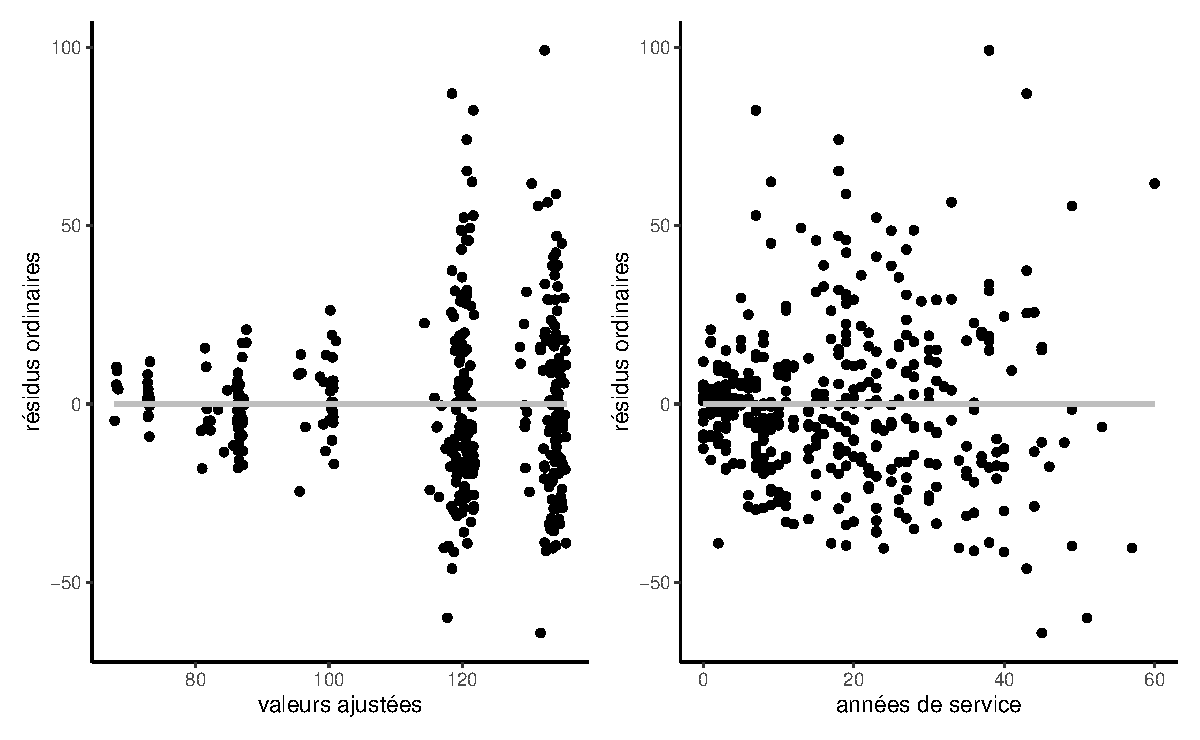
\includegraphics[width=0.85\textwidth,height=\textheight]{regression-lineaire_files/figure-pdf/fig-zerocor-1.pdf}

}

\caption{\label{fig-zerocor}Diagramme des résidus en fonction des
valeurs ajustées (à gauche) et de la variable explicative
\texttt{service} (à droite) pour la régression linéaire des données
\texttt{college}. L'ordonnée à l'origine et la pente des régressions
linéaires simples sont nulles.}

\end{figure}%

\end{corollary}

\begin{corollary}[Moyenne des résidus
nulle]\protect\hypertarget{cor-zeromean}{}\label{cor-zeromean}

Puisque le produit scalaire est zéro, la moyenne de \(\boldsymbol{e}\)
doit être zéro pour autant que \(\mathbf{1}_n\) est dans l'espace
linéaire engendré par \(\mathbf{X}\).

\begin{Shaded}
\begin{Highlighting}[]
\NormalTok{mod }\OtherTok{\textless{}{-}} \FunctionTok{lm}\NormalTok{(salaire }\SpecialCharTok{\textasciitilde{}}\NormalTok{ sexe }\SpecialCharTok{+}\NormalTok{ echelon }\SpecialCharTok{+}\NormalTok{ domaine }\SpecialCharTok{+}\NormalTok{ service, }\AttributeTok{data =}\NormalTok{ college)}
\CommentTok{\# Corrélation nulle}
\FunctionTok{with}\NormalTok{(college, }\FunctionTok{cor}\NormalTok{(}\FunctionTok{resid}\NormalTok{(mod), service))}
\CommentTok{\#\textgreater{} [1] 1.26e{-}17}
\FunctionTok{cor}\NormalTok{(}\FunctionTok{resid}\NormalTok{(mod), }\FunctionTok{fitted}\NormalTok{(mod))}
\CommentTok{\#\textgreater{} [1] 2.32e{-}17}
\CommentTok{\# Moyenne des résidus ordinaires est nulle}
\FunctionTok{mean}\NormalTok{(}\FunctionTok{resid}\NormalTok{(mod))}
\CommentTok{\#\textgreater{} [1] {-}5.6e{-}16}
\end{Highlighting}
\end{Shaded}

Puisque les aléas avaient moyenne théorique de zéro, on veut forcer les
résidus ordinaires à avoir une moyenne empirique de zéro en incluant
l'ordonnée à l'origine.

\end{corollary}

\begin{refremark}[Invariance]
Une conséquence directe de l'expression de l'estimateur des MCO en terme
de matrice de projection est que les valeurs ajustées \(\widehat{y}_i\)
pour deux matrices de modèle \(\mathbf{X}_a\) et \(\mathbf{X}_b\) sont
les mêmes si elles engendrent le même espace linéaire, comme dans
Exemple~\ref{exm-baumann-dummies}; seule l'interprétation des
coefficients change. Si nous incluons une ordonnée à l'origine, nous
obtenons le même résultat si les colonnes explicatives sont centrées sur
la moyenne.

\begin{Shaded}
\begin{Highlighting}[]
\NormalTok{modA }\OtherTok{\textless{}{-}} \FunctionTok{lm}\NormalTok{(salaire }\SpecialCharTok{\textasciitilde{}}\NormalTok{ sexe }\SpecialCharTok{+}\NormalTok{ echelon }\SpecialCharTok{+}\NormalTok{ service, }\AttributeTok{data =}\NormalTok{ college)}
\NormalTok{modB }\OtherTok{\textless{}{-}} \FunctionTok{lm}\NormalTok{(salaire }\SpecialCharTok{\textasciitilde{}} \DecValTok{0} \SpecialCharTok{+}\NormalTok{ sexe }\SpecialCharTok{+}\NormalTok{ echelon }\SpecialCharTok{+}\NormalTok{ service, }\CommentTok{\# Enlever l\textquotesingle{}ordonnée à l\textquotesingle{}origine}
           \AttributeTok{data =}\NormalTok{ college }\SpecialCharTok{|\textgreater{}} 
\NormalTok{            dplyr}\SpecialCharTok{::}\FunctionTok{mutate}\NormalTok{(}\AttributeTok{service =} \FunctionTok{scale}\NormalTok{(service)), }\CommentTok{\# Centrer{-}réduire une variable}
           \AttributeTok{contrasts =} \FunctionTok{list}\NormalTok{(}\AttributeTok{echelon =}\NormalTok{ contr.sum)) }\CommentTok{\# changer la paramétrisation}
\FunctionTok{head}\NormalTok{(}\FunctionTok{model.matrix}\NormalTok{(modA), }\AttributeTok{n =} \DecValTok{3}\NormalTok{L)}
\CommentTok{\#\textgreater{}   (Intercept) sexefemme echelonaggrege echelontitulaire service}
\CommentTok{\#\textgreater{} 1           1         0              0                1      18}
\CommentTok{\#\textgreater{} 2           1         0              0                1      16}
\CommentTok{\#\textgreater{} 3           1         0              0                0       3}
\FunctionTok{head}\NormalTok{(}\FunctionTok{model.matrix}\NormalTok{(modB), }\AttributeTok{n =} \DecValTok{3}\NormalTok{L)}
\CommentTok{\#\textgreater{}   sexehomme sexefemme echelon1 echelon2 service}
\CommentTok{\#\textgreater{} 1         1         0       {-}1       {-}1  0.0296}
\CommentTok{\#\textgreater{} 2         1         0       {-}1       {-}1 {-}0.1241}
\CommentTok{\#\textgreater{} 3         1         0        1        0 {-}1.1237}
\CommentTok{\# Invariance du modèle}
\FunctionTok{isTRUE}\NormalTok{(}\FunctionTok{all.equal}\NormalTok{(}\FunctionTok{fitted}\NormalTok{(modA), }\FunctionTok{fitted}\NormalTok{(modB)))}
\CommentTok{\#\textgreater{} [1] TRUE}
\end{Highlighting}
\end{Shaded}

\label{rem-invariance}

\end{refremark}

La valeur de \(\widehat{\boldsymbol{\beta}}\) est telle qu'elle maximise
la corrélation entre \(\boldsymbol{y}\) et \(\widehat{\boldsymbol{y}}\).
Dans le cas d'une variable catégorielle unique, nous obtiendrons des
valeurs ajustées \(\widehat{y}\) qui correspondent à la moyenne de
l'échantillon de chaque groupe.

\label{rem-geometry}

\end{refremark}

\subsection{Résidus}\label{ruxe9sidus}

Les résidus sont les prédictions des aléas \(\varepsilon\), et
représentent la différence entre la valeur observée de la réponse
\(Y_i\) et sa prédiction. Les résidus ordinaires sont définis comme
\begin{align*}
e_i=Y_i-\widehat{Y}_i, \qquad i =1, \ldots, n.
\end{align*} La somme des résidus ordinaire est toujours zéro par
construction si on inclut une ordonnée à l'origine, ce qui donne que
\(\overline{e} = 0\).

Toutes les observations ne contribuent pas de la même manière à
l'ajustement de l'hyperplan ajusté. La géométrie des moindres carrés
montre que les résidus sont orthogonaux aux valeurs ajustées, et que
\(\boldsymbol{e} = (\mathbf{I}_n-\mathbf{H}_{\mathbf{X}})\boldsymbol{Y}\),
où
\(\mathbf{H}_{\mathbf{X}}=\mathbf{X}(\mathbf{X}^\top\mathbf{X})^{-1}\mathbf{X}^\top\)
est une matrice de projection de dimension \(n \times n\) qui génère un
sous-espace vectoriel de dimension \((p+1)\) décrouvrant toutes les
combinaisons linéaires des colonnes de \(\mathbf{X}\), dénoté
\(\mathscr{S}(\mathbf{X})\). Si
\(\mathsf{Va}(\boldsymbol{Y}) = \sigma^2\mathbf{I}_n\), il en découle
que
\(\mathsf{Va}(\boldsymbol{e})=\sigma^2(\mathbf{I}_n-\mathbf{H}_{\mathbf{X}})\)
parce que \(\mathbf{I}_n-\mathbf{H}_{\mathbf{X}}\) est une matrice de
projection orthogonale, donc idempotente et symmérique. Puisque la
matrice \(\mathbf{I}_n-\mathbf{H}_{\mathbf{X}}\) a rang \(n-p-1\), les
résidus ordinaires ne sont pas indépendants les uns des autres.

Si les aléas sont indépendants et homoscédastiques, les résidus
ordinaires \(e_i\) ont une variance de \(\sigma^2(1-h_{i})\), où le
terme de levier
\(h_i =(\mathbf{H}_{\mathbf{X}})_{ii} = \mathbf{x}_i (\mathbf{X}^\top\mathbf{X})^{-1}\mathbf{x}_i\)
est le \(i\)e élément de la diagonale de la matrice de projection
\(\mathbf{H}_{\mathbf{X}}\) et \(\mathbf{x}_i\) est comme à l'accoutumée
la \(i\)e ligne de la matrice du modèle qui correspond à l'observation
\(i\).

Nous concluons donc que les résidus ordinaires n'ont pas tous le même
écart-type et qu'ils ne sont pas indépendants. Ceci est problématique,
car nous ne pouvons pas faire de comparaisons de leurs lois: les points
ayant un faible effet de levier s'écartent davantage du modèle ajusté
que les autres. Pour pallier ce problème, nous pouvons normaliser les
résidus de façon à ce que chacun ait la même variance sous l'hypothèse
nulle d'erreurs homoscédastiques indépendantes --- les termes d'effet de
levier \(h_i\) sont facilement calculés à partir de la matrice du modèle
\(\mathbf{X}\).

La seule question qui subsiste est celle de l'estimation de la variance.
Si nous utilisons la \(i\)e observation pour estimer à la fois le résidu
et la variance, nous introduisons une dépendance supplémentaire. Une
meilleure solution consiste à supprimer la \(i\)e observation et à
réajuster le modèle avec les \(n-1\) observations restantes pour obtenir
\(S^2_{(-i)}\) (il existe des formules explicites qui font qu'il n'est
pas nécessaire d'ajuster \(n\) modèles linéaires). Les résidus
studentisés externes \(r_i = e_i/\{s_{(-i)}(1-h_i)\}\), également
appelés résidus studentisés par la méthode du canif, ne sont pas
indépendants, mais ils sont une loi marginale identique de Student avec
\(n-p-2\) degrés de liberté. Ils peuvent être obtenus dans \textbf{R}
avec la commande \texttt{rstudent}.

Quand utiliser quels résidus? Par construction, le vecteur des résidus
ordinaires \(\boldsymbol{e}\) est orthogonal aux valeurs ajustées
\(\widehat{\boldsymbol{y}}\) et également à chaque colonne de la matrice
du modèle \(\mathbf{X}\): cela signifie qu'une simple régression
linéaire de \(\boldsymbol{e}\) avec n'importe laquelle de ces
covariables donne une ordonnée à l'origine et une pente toutes deux
nulles. Ainsi, les modèles résiduels dus à des interactions oubliées, à
des termes non linéaires, etc. pourraient être détectés à partir de
diagrammes de paires de résidus ordinaires en fonction des variables
explicatives.

Bien que les résidus studentisés externes \(r_i\) ne soient pas
orthogonaux, ils ne sont pas très différents quand \(n\) est grand par
rapport à \(p\). On peut utiliser les résidus \(\boldsymbol{r}\) pour
vérifier l'égalité de la variance et les hypothèses de distribution (par
exemple, à l'aide d'un diagramme quantile-quantile).

\begin{definition}[Coefficient de
détermination]\protect\hypertarget{def-r2}{}\label{def-r2}

Lorsque nous spécifions un modèle, les aléas
\(\boldsymbol{\varepsilon}\) servent à tenir compte du fait qu'aucune
relation linéaire exacte ne caractérise les données Une fois que nous
avons ajusté un modèle, nous estimons la variance \(\sigma^2\); on peut
alors se demander quelle part de la variance totale de l'échantillon est
expliquée par le modèle.

La somme totale des carrés, définie comme la somme des carrés des
résidus du modèle à ordonnée à l'origine uniquement, sert de comparaison
--- le modèle le plus simple que nous puissions trouver impliquerait
chaque observation par la moyenne de l'échantillon de la réponse, ce qui
donne la variance expliquée
\(\mathsf{SC}_c = \sum_{i=1}^n (y_i - \overline{y})^2\). Nous pouvons
ensuite comparer la variance des données originales avec celle des
résidus du modèle avec la matrice de covariables \(\mathbf{X}\), définie
comme \(\mathsf{SC}_e =\sum_{i=1}^n e_i^2\) avec
\(e_i = y_i - \widehat{\beta}_0 - \sum_{j=1}^p \widehat{\beta}_jX_j\).
Nous définissons le coefficient de détermination \(R^2\), comme suit
\begin{align*}
R^2 &=1- \frac{\mathsf{SC}_e}{\mathsf{SC}_c} = \frac{\sum_{i=1}^n (y_i - \overline{y})^2- \sum_{i=1}^n e_i^2}{\sum_{i=1}^n (y_i - \overline{y})^2}.
\end{align*} Une autre décomposition montre que
\(R^2 = \mathsf{cor}^2(\boldsymbol{y}, \widehat{\boldsymbol{y}})\),
c'est-à-dire que le coefficient de détermination peut être interprété
comme le carré de la corrélation linéaire de Pearson
(Définition~\ref{def-correlation-Pearson}) entre la réponse
\(\boldsymbol{y}\) et les valeurs ajustées \(\widehat{\boldsymbol{y}}\).

\end{definition}

Il est important de noter que le \(R^2\) n'est pas un critère de qualité
de l'ajustement, tout comme la log-vraisemblance. En effet, certain
phénomènes sont intrinsèquement complexes et même un bon modèle ne
parviendra pas à rendre compte d'une grande partie de la variabilité de
la réponse. Ce n'est pas non plus parce que le \(R^2\) est faible que
\(Y\) et et les variables explicatives \(X_j\) sont indépendantes, comme
l'illustre la Figure~\ref{fig-datasaurus}.

En outre, il est possible de gonfler la valeur de \(R^2\) en incluant
davantage de variables explicatives et en rendant le modèle plus
complexe, ce qui améliore la vraisemblance et \(R^2\). En effet, le
coefficient n'est pas décroissant dans la dimension de \(\mathbf{X}\),
de sorte qu'un modèle comportant \(p+1\) de covariables aura
nécessairement des valeurs de \(R^2\) plus élevées que si l'on
n'incluait que \(p\) de ces variables explicatives. Pour comparer les
modèles, il est préférable d'utiliser des critères d'information ou de
s'appuyer sur la performance prédictive si tel est l'objectif de la
régression. Enfin, un modèle avec un \(R^2\) élevé peut impliquer une
corrélation élevée, mais
\href{http://www.tylervigen.com/spurious-correlations}{la relation peut
être fallacieuse} : la régression linéaire ne produit pas de modèles
causaux!

\subsection{Colinéarité}\label{colinuxe9arituxe9}

Le postulat de linéarité peut être interprétée au sens large comme
signifiant que toutes les covariables pertinentes ont été incluses et
que leur effet est correctement spécifié dans l'équation de la moyenne.
L'ajout de covariables superflues à un modèle a un impact limité: si la
corrélation (partielle) entre un vecteur colonne \(\boldsymbol{X}_k\) et
la variable réponse \(\boldsymbol{Y}\) est nulle, alors \(\beta_k=0\) et
le coefficient estimé \(\widehat{\beta}_k \approx 0\) parce que les
estimateurs des moindres carrés sont sans biais. Si nous incluons de
nombreuses variables inutiles, disons \(k\), le manque de parcimonie
peut toutefois rendre l'interprétation plus difficile. Le prix à payer
pour inclure \(k\) de variables explicatives supplémentaires est une
augmentation de la variance des estimateurs
\(\widehat{\boldsymbol{\beta}}\).

Dans les études observationnelles, il est néanmoins préférable d'inclure
davantage de variables que d'oublier des variables explicatives clés: si
nous omettons une variable prédictive importante, son effet peut être
capturé par d'autres \textbf{variables confondantes}, qui sont corréléws
avec à la fois les variables omises et la réponse et qui causent les
deux. Par exemple, le modèle linéaire simple (ou le test \(t\) à deux
échantillons) pour le salaire en fonction du sexe pour les données de
salaires dans un collège n'est pas valide parce que l'échelon académique
est un facteur confondant pour les différences selon le sexe. Comme il y
a plus d'hommes que de femmes professeurs titulaires, la différence de
salaire moyen entre les hommes et les femmes est plus élevée de
l'échantillon qu'elle ne l'est réellement. Une façon d'en tenir compte
est d'inclure des variables de contrôle (telles que l'échelon), dont
l'effet ne nous intéresse pas forcément, mais qui sont nécessaires pour
que le modèle soit adéquat. Nous aurions également pu utiliser la
stratification, c'est-à-dire tester la discrimination salariale au sein
de chaque échelon académique. C'est la raison pour laquelle des
variables sociodémographiques (sexe, âge, niveau d'éducation, etc.) sont
collectées dans le cadre des études.

Un modèle linéaire n'est pas un {[}modèle causal{]}
(https://xkcd.com/552/): il ne fait que capturer la corrélation linéaire
entre une variable explicative et la réponse. Lorsqu'il y a plus d'une
variable explicative, l'effet de \(X_j\) est fonction de ce qui n'a pas
déjà été expliqué par les autres variables explicatives, disons
\(\boldsymbol{X}_{-j}\). Ainsi, si nous ne parvenons pas à rejeter
\(\mathscr{H}_0:\beta_j=0\) en faveur de l'alternative
\(\mathscr{H}_1 : \beta_j \neq 0\), nous pouvons seulement dire qu'il
n'y a pas d'association \emph{linéaire} significative entre \(X_j\) et
\(Y\) une fois que l'effet des autres variables incluses dans le modèle
a été pris en compte. Il existe donc deux scénarios: soit la réponse
n'est pas corrélée à \(X_j\) (cas inintéressant, mais facile à repérer
en traçant les deux ou en calculant la corrélation linéaire), soit il
existe une forte corrélation entre \(X_j\) et à la fois la réponse \(Y\)
et (certaines) des autres variables explicatives \(X_1, \ldots, X_p\).
Ce problème est appelé (multi)\textbf{colinéarité}.

L'un des inconvénients de la colinéarité est la diminution de la
précision des estimateurs de paramètres. En présence de variables
explicatives colinéaires, de nombreuses combinaisons linéaires des
covariables représentent presque aussi bien la réponse. En raison du
manque (ou presque) d'identifiabilité, les coefficients estimés
deviennent numériquement instables, ce qui entraîne une augmentation des
erreurs-type des paramètres. Les valeurs prédites ou ajustées ne sont
pas affectées. En général, les coefficients de régression peuvent
changer radicalement lorsque de nouvelles observations sont incluses
dans le modèle, ou lorsque nous incluons ou supprimons des variables
explicatives. Les coefficients \(\beta\) individuels peuvent ne pas être
statistiquement significatifs, mais le test \(F\) global indiquera que
certaines covariables sont pertinentes pour expliquer la réponse.
Toutefois, ce serait également le cas s'il y avait des prédicteurs avec
un signal fort, de sorte que ni l'un ni l'autre n'est susceptible d'être
utile pour détecter les problèmes.

Le \textbf{diagramme de régression partielle} montre à l'aide d'un nuage
de points la relation entre la réponse \(Y\) et une variable explicative
\(X_j\) après la prise en compte de l'effet linéaire des autres
variables. Il est obtenu en faisant une régressant à tour de rôle
\(X_j\) et \(Y\) sur les autres colonnes de la matrice du modèle, et en
calculant les résidus. Le théorème de Frisch--Waugh--Lovell montre que
la pente \(\widehat{\beta}_j\) de la régression linéaire simple entre
les résidus \(\boldsymbol{e}_{Y}^{-j}\) et \(\boldsymbol{e}_{X_j}^{-j}\)
est la même que celle du modèle complet. Si on ne voit pas de relation
linéaire dans le graphique (pente presque nulle) et que la corrélation
entre \(X_j\) et \(Y\) était très forte, cela est typiquement indicateur
de colinéarité.

Une idée similaire peut être utilisée pour voir quelle part de \(X_j\)
est déjà expliquée par les autres variables. Nous définissons le facteur
\textbf{facteur d'inflation de la variance} comme
\(\mathsf{FIV}(j)=(1-R^2(j))^{-1}\), où \(R^2(j)\) est le coefficient de
détermination du modèle obtenu en régressant \(X_j\) sur toutes les
autres variables explicatives, c'est-à-dire, \begin{align*}
X_j = \beta^{\star}_0 + \beta^{\star}_1 X_1 + \cdots + \beta^{\star}_{j-1} X_{j-1} + \beta^{\star}_{j+1} X_{j+1} + \cdots + \beta^{\star}_pX_p + \varepsilon^{\star}
\end{align*} Par définition, \(R^2(j)\) donne la proportion de la
variance de \(X_j\) expliquée par les autres variables explicatives. Un
facteur d'inflation de la variance élevé est un indicateur de
colinéarité: typiquement les valeurs avec une corrélation de plus de
90\%, ou \(\mathsf{FIV}>10\), nécessitent une attention particulière.
Les valeurs dans les centaines ou les milliers représentent des cas
pathologiques. Pour les variables catégorielles, la définition du
facteur d'inflation de la variance donnerait normalement une valeur
différente pour chaque niveau; une alternative est le facteur
d'inflation de la variance généralisée (\citeproc{ref-Fox:1992}{Fox et
Monette 1992}).

Que doit-on faire s'il y a de la colinéarité ? Si l'objectif de l'étude
est de développer un modèle prédictif et que nous ne sommes pas
intéressés par les paramètres eux-mêmes, alors nous n'avons rien à
faire. La colinéarité n'est pas un problème pour le modèle global: c'est
seulement un problème pour les effets individuels des variables. Leur
effet conjoint est toujours présent dans le modèle, quelle que soit la
manière dont les effets individuels sont combinés.

Si nous nous intéressons aux estimations des paramètres individuels, par
exemple pour voir comment (et dans quelle mesure) les variables
prédictives expliquent le comportement de \(Y\), les choses se
compliquent. La colinéarité n'affecte que les variables qui sont
fortement corrélées les unes aux autres, de sorte que nous ne nous
préoccupons que si elle affecte une ou plusieurs des variables qui nous
intéressent. Il n'y a malheureusement pas de bonne solution à ce
problème. On pourrait

\begin{itemize}
\tightlist
\item
  essayer d'obtenir plus de données, afin de réduire les effets de
  colinéarité apparaissant dans des échantillons spécifiques ou dus à la
  petite taille de l'échantillon.
\item
  créer un score composite en combinant d'une manière ou d'une autre les
  variables présentant une colinéarité.
\item
  supprimer une ou plusieurs des variables colinéaires. Vous devez en
  revanche faire attention à ne pas vous retrouver avec un modèle mal
  spécifié.
\item
  utiliser la régression pénalisée si \(\mathbf{X}^\top\mathbf{X}\)
  n'est (presque) pas inversible, cela peut restaurer l'unicité de la
  solution. Les pénalités introduisent un biais, mais peuvent réduire la
  variance des estimateurs \(\boldsymbol{\beta}\). Les choix populaires
  incluent la régression en crête (avec une pénalité de \(l_2\)), lasso
  (pénalité de \(l_1\)), mais ceux-ci requièrent un ajustement pour
  l'inférence post-sélection
\end{itemize}

Quelle que soit la méthode utilisée, il est important de comprendre
qu'il peut être très difficile (et parfois impossible) d'isoler l'effet
individuel d'une variable explicative fortement corrélée avec d'autres.

\begin{example}[Colinéarité des données de
\texttt{college}]\protect\hypertarget{exm-collegedatcollineaire}{}\label{exm-collegedatcollineaire}

On considère l'analyse des données sur l'inéquité salariale dans un
college, en incluant cette fois \texttt{annees}, le nombre d'années
depuis l'obtiention du doctorat. On peut penser que, à moins qu'un(e)
professeur(e) ait entamé sa carrière dans une autre institution
d'enseignement, le nombre d'années de service sera fortement lié à ces
derniers. De fait, la corrélation linéaire entre \texttt{service} et
\texttt{annees} est 0.91. Cette corrélation n'est pas problématique
puisque le \(\mathsf{FIV}\) pour \(\texttt{sexe}\) (voir le
Tableau~\ref{tbl-vif-college}) n'est pas élevé et l'inclusion sert à
éviter les variables confondantes et réduire l'incertitude.

\begin{figure}[ht!]

\centering{

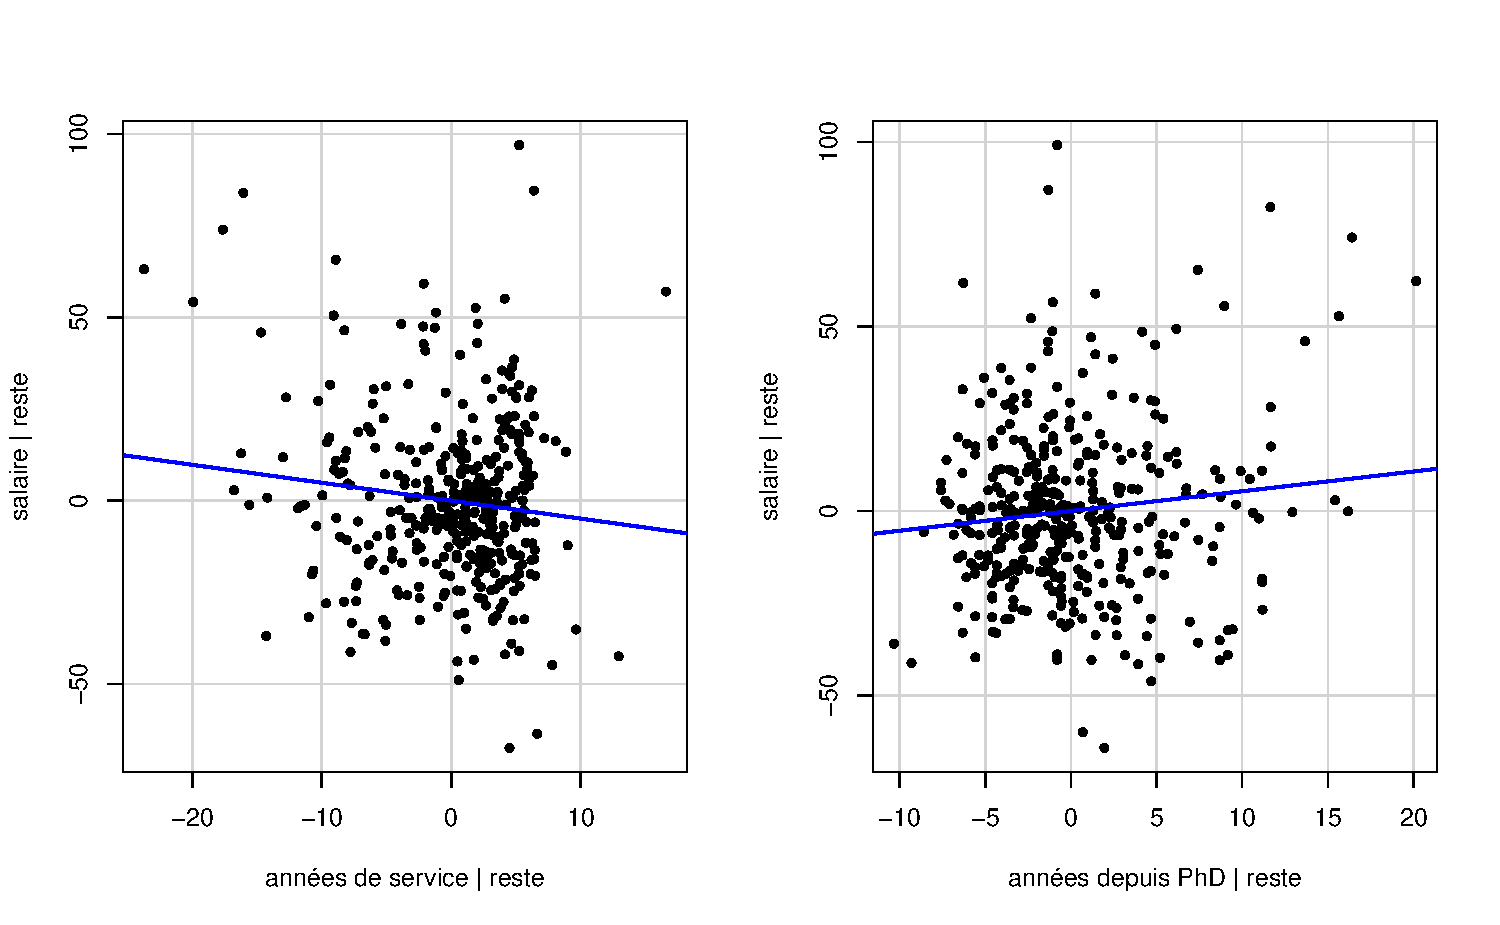
\includegraphics[width=1\textwidth,height=\textheight]{regression-lineaire_files/figure-pdf/fig-addedvariableplots-1.pdf}

}

\caption{\label{fig-addedvariableplots}Diagramme de régression partielle
pour le nombre d'années de service et le nombre d'années depuis le
doctorat.}

\end{figure}%

\begin{longtable}[]{@{}rrrrr@{}}

\caption{\label{tbl-vif-college}Facteur d'inflation de la variance
généralisés pour les données \texttt{college}.}

\tabularnewline

\toprule\noalign{}
echelon & domaine & sexe & service & annees \\
\midrule\noalign{}
\endhead
\bottomrule\noalign{}
\endlastfoot
2.01 & 1.06 & 1.03 & 5.92 & 7.52 \\

\end{longtable}

\end{example}

\subsection{Levier et aberrances}\label{levier-et-aberrances}

L'effet de levier \(h_i\) de l'observation \(i\) mesure son impact sur
l'ajustement par les moindres carrés, puisque nous pouvons écrire
\(h_i = \partial \widehat{y}_i/\partial y_i\). Les valeurs de l'effet de
levier nous indiquent l'impact de chaque point sur l'ajustement : elles
sont strictement positives, avec une borne inférieure de \(1/n\) et une
borne supérieure de \(1\). La somme des leviers est
\(\sum_{i=1}^n h_i=p+1\) : dans un bon modèle, chaque point a
approximativement la même contribution, avec un poids moyen de
\((p+1)/n\).

Les points à fort effet de levier sont ceux qui présentent des
combinaisons inhabituelles de variables explicatives. Une observation
\textbf{influente} (\(h_i\approx 1\)) tire l'hyperplan ajusté vers
elle-même de sorte que \(\hat{y}_i \approx y_i\). En règle générale, les
points avec \(h_i> 2(p+1)/n\) doivent être examinés de près.

Il est important de faire la distinction entre les observations
\textbf{influentes} (qui ont une valeur \(\mathbf{x}\) inhabituelle,
c'est-à-dire éloignée de la moyenne générale) et les \textbf{aberrances}
(valeur inhabituelle de la réponse \(y\)). Si une observation est à la
fois une valeur aberrante et a un effet de levier élevé, elle est
problématique.

\begin{figure}[ht!]

\centering{

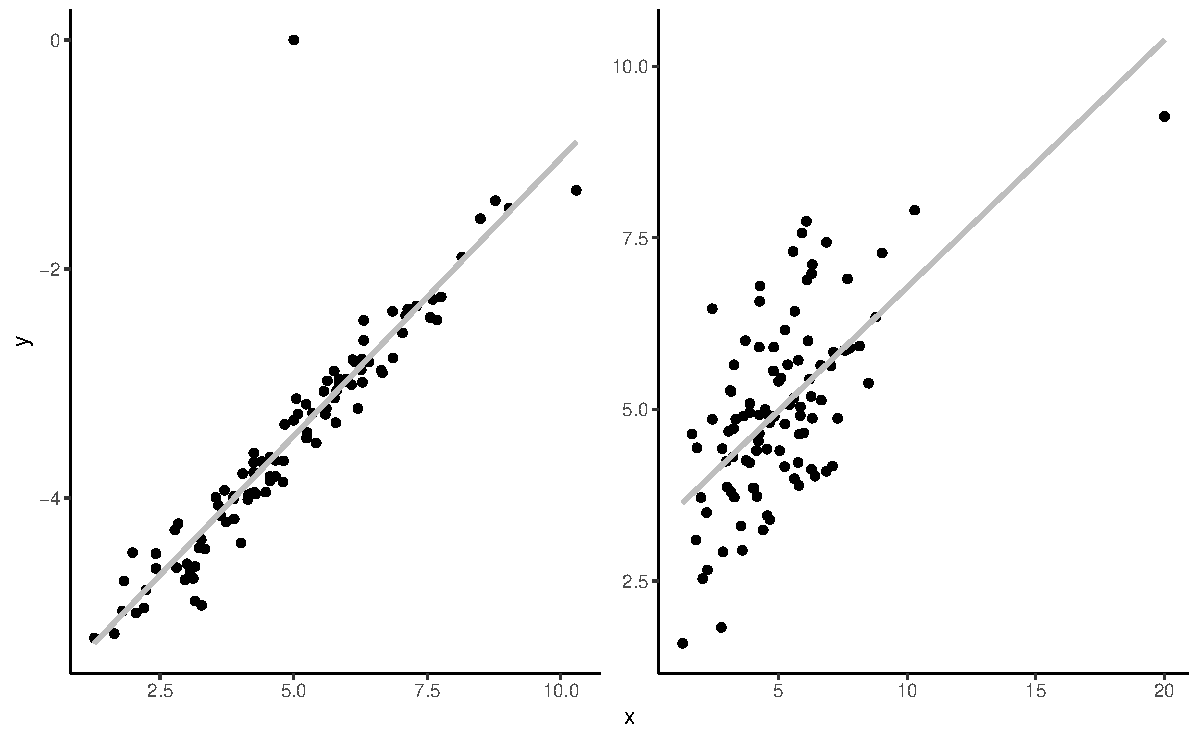
\includegraphics[width=0.85\textwidth,height=\textheight]{regression-lineaire_files/figure-pdf/fig-outliers-1.pdf}

}

\caption{\label{fig-outliers}Valeur aberrante (gauche) et observation
influente (droite, valeur de \(x\) la plus à droite).}

\end{figure}%

Si les observations influentes peuvent être détectées en inspectant le
levier de chaque observation, les valeurs aberrantes sont plus
difficiles à diagnostiquer. Une valeur aberrante se distingue du reste
des observations, soit parce qu'elle a une valeur de réponse habituelle,
soit parce qu'elle se situe loin de la surface de régression. En gros,
une valeur aberrante est une valeur inhabituelle de \(Y\) pour une
combinaison donnée de \(\mathbf{X}\) qui se distingue des autres. Les
valeurs aberrantes peuvent être détectées au cours de l'analyse
exploratoire des données ou dans les diagrammes de résidus (valeurs
élevées de \(|e_i|\) dans les diagrammes des valeurs ajustées par
rapport aux valeurs résiduelles) ou dans les diagrammes de régression
partielle. On pourrait éventuellement tester si un résidu studentisé
externe est une valeur aberrante (en tenant compte du fait que nous ne
prendrions en considération que les valeurs les plus élevées). On peut
également considérer la distance de Cook, \(C_j\), une statistique
donnant la distance à l'échelle entre les valeurs ajustées
\(\hat{\boldsymbol{y}}\) et les valeurs ajustées pour le modèle avec
toutes les observations sauf la \(j\)e, \(\hat{\boldsymbol{y}}^{(-j)}\),
\begin{align*}
C_j = \frac{1}{(p+1)S^2} \sum_{i=1}^n \left\{\hat{y}_i - \hat{y}_{i}^{(-j)}\right\}^2
\end{align*} Des valeurs élevées de \(C_j\) indiquent que son résidu
ordinaire \(e_j\) est important par rapport aux autres observations ou
que son effet de levier \(h_j\) est élevé. Une règle empirique consiste
à considérer les points pour lesquels \(C_j > 4/(n-p-1)\). En pratique,
si deux observations sont aberrantes et se situent dans la même région,
leur distance de Cook sera réduite de moitié.

Les observations aberrantes et influentes ne doivent pas être négligées
parce qu'elles ne sont pas conformes au modèle, mais doivent faire
l'objet d'un examen plus approfondi. Elles peuvent motiver une
modélisation plus poussée des caractéristiques non prises en compte. Il
est également utile de vérifier les erreurs d'enregistrement dans les
données (qui peuvent être écartées sans risque). Dans les très grands
échantillons, l'impact d'une seule valeur aberrante est, espérons-le,
limité. Les transformations de la réponse peuvent contribuer à réduire
le caractère aberrant. Sinon, il est possible d'utiliser d'autres
fonctions objectives que le critère des moindres carrés ordinaires
(telles que celles employées dans la régression robuste); celles-ci
pondèrent les observations extrêmes, au détriment de l'efficacité.

\section{Postulats du modèle et
diagnostics}\label{postulats-du-moduxe8le-et-diagnostics}

Cette section passe en revue les postulats du modèle énoncés pour
permettre l'inférence statistique à l'aide du modèle linéaire et des
différents résidus qui servent d'éléments de base pour les diagnostics
graphiques. Nous étudions les conséquences de la violation de ces
postulats et décrivons des stratégies d'atténuation potentielles, dont
beaucoup sont abordées dans d'autres chapitres.

Jusqu'à présent, nous avons ajusté des modèles et testé la
significativité des coefficients sans valider notre modèle. La fiabilité
des valeurs \(p\) et des intervalles de confiance dépend de la validité
(approximative) des postulats du modèle, qui découlent toutes de
l'hypothèse sur les alés, supposée indépendantes et identiquement
distribuées avec
\(\varepsilon_i \stackrel{\cdot}{\sim} \mathsf{normale}(0, \sigma^2)\).
Cette description mathématique compacte peut être décomposée en quatre
postulats principaux: Il y a quatre postulats principaux du modèle
linéaire de la forme
\[Y_i \mid \mathbf{x}_i \sim \mathsf{normale}(\mathbf{x}_i\boldsymbol{\beta}, \sigma^2)\]

\begin{itemize}
\tightlist
\item
  linéarité et additivité: la moyenne de \(Y_i \mid \mathbf{x}_i\) est
  \(\beta_0 + \beta_1x_{i1} + \cdots + \beta_p x_{ip}\),
\item
  homoscédasticité: la variance des observations \(\sigma^2\) est
  constante,
\item
  indépendence des observations (conditionnellement aux covariables),
\item
  normalité.
\end{itemize}

Lorsque nous effectuons un test d'hypothèse et que nous ne rejetons pas
l'hypothèse nulle, c'est soit parce qu'elle est vraie, soit par manque
de preuves. Il en va de même pour la vérification de la validité des
postulats du modèle: le raisonnement scientifique veut que nous ne
puissions pas savoir avec certitude si ces derniers sont vrais. Notre
stratégie consiste donc à utiliser les implications des hypothèses du
modèle linéaire pour créer des outils de diagnostics graphiques, afin de
s'assurer qu'il n'y a pas de violation flagrante des postulats.
Toutefois, il est important de se garder de surinterpréter les
diagnostics graphiques: l'oeil humain est très doué pour trouver des
schémas inexistants.

\subsection{Postulat de linéarité et
d'additivité}\label{postulat-de-linuxe9arituxe9-et-dadditivituxe9}

Le postulat de linéarité signifie que le modèle moyen est correctement
spécifié, que toutes les covariables pertinentes ont été incluses et que
leur effet est correctement spécifié (y compris les effets non linéaires
et les interactions). L'additivité sous-tend que le modèle peut être
exprimé comme la somme de moyenne plus aléa. Pour vérifier que la
surface de réponse du modèle linéaire est adéquate, nous dessinons un
nuage de points de \(e_i\) en fonction de \(\widehat{y}_i\) ou
\(x_{ij}\) (pour \(j=1, \ldots, p\)). Étant donné que la corrélation
linéaire entre \(\boldsymbol{e}\) et \(\widehat{\boldsymbol{y}}\) (ou
\(\boldsymbol{e}\) et \(\mathbf{X}_j\)) est nulle par construction, les
modèles (par exemple, tendance quadratique, cycles, points de
changement) sont indicatifs d'une mauvaise spécification du modèle pour
la moyenne. Il est possible d'ajouter une courbe de lissage de tels
effets. La Figure~\ref{fig-regdiaglin} montre trois diagrammes de
résidus. On cherche une tendance locale dans l'axe des ordonnées \(y\),
pas sur l'axe des abcisses.

\begin{figure}[ht!]

\centering{

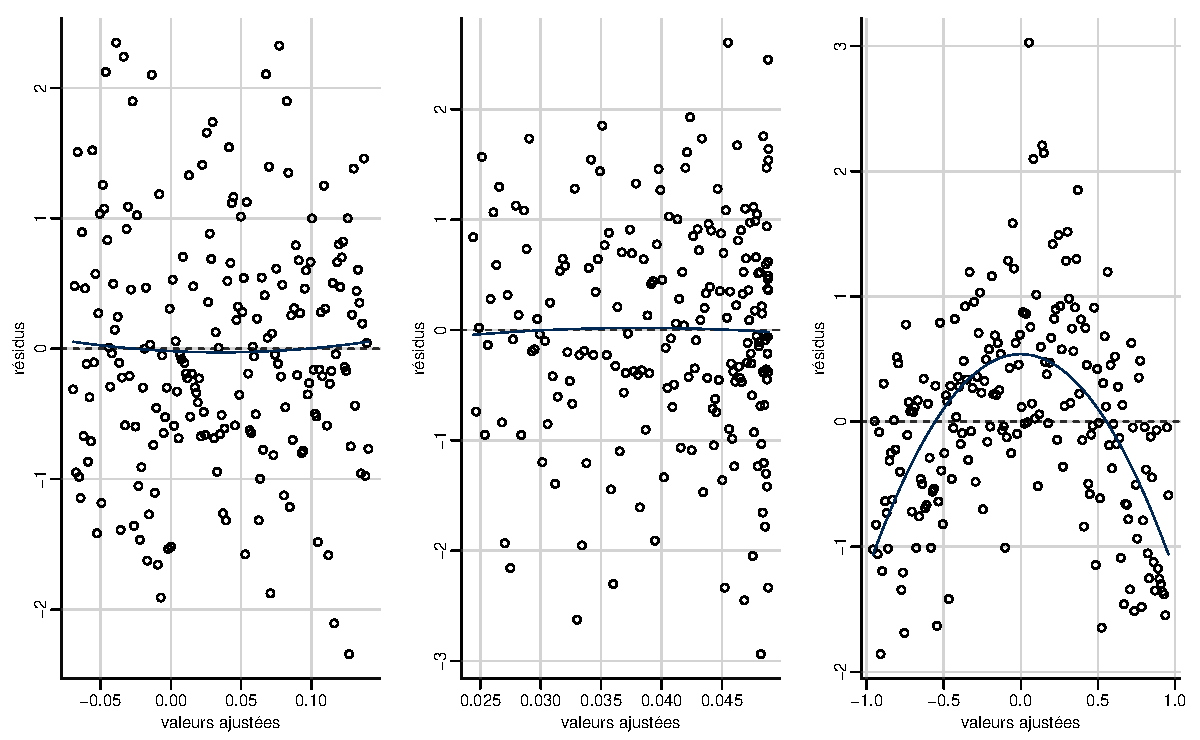
\includegraphics[width=0.85\textwidth,height=\textheight]{regression-lineaire_files/figure-pdf/fig-regdiaglin-1.pdf}

}

\caption{\label{fig-regdiaglin}Diagrammes des résidus par rapport aux
valeurs ajustées. Les deux premiers diagrammes ne montrent aucun écart
par rapport à la linéarité (moyenne locale nulle). Le troisième
diagramme montre une tendance quadratique évidente, ce qui suggère que
le modèle moyen est mal spécifié. Notez que la distribution de la valeur
ajustée n'est pas nécessairement uniforme, comme dans le deuxième
panneau.}

\end{figure}%

S'il existe une structure résiduelle dans les graphiques des résidus
ordinaires en fonction (a) des valeurs ajustées ou (b) des variables
explicatives, un modèle plus complexe peut être ajusté, y compris un
contenant des interactions, des fonctions non linéaires, etc. Si l'effet
d'une variable explicative est clairement non linéaire et compliqué, des
termes de lissage peuvent être ajoutés (nous ne couvrirons pas les
modèles additifs généralisés dans ce cours).

La représentation graphique des résidus en fonction des variables
explicatives omises peut également servir à vérifier que tout le pouvoir
explicatif de la covariable omise est déjà expliqué par les colonnes de
\(\mathbf{X}\).

Si une variable importante a été omise et n'est pas disponible dans
l'ensemble de données, l'effet de cette variable est capturé à la fois
par les erreurs (la partie orthogonale à la matrice du modèle
\(\mathbf{X}\), c'est-à-dire inexpliquée par les covariables incluses
dans le modèle) et la partie restante est capturée par d'autres
variables explicatives du modèle qui sont corrélées avec la variable
omise. Ces variables peuvent agir comme des facteurs de confusion. Dans
les deux cas, il n'y a pas grand-chose à faire si les données relatives
à la variable omise ne sont pas disponibles, mais des connaissances
spécifiques au sujet peuvent aider à donner un sens aux résultats.

\subsection{Postulat
d'homoscédasticité}\label{postulat-dhomoscuxe9dasticituxe9}

Si la variance des aléas est la même pour toutes les observations
(homoscédasticité), celle des observations \(Y\) est également
constante. Les scénarios les plus courants d'hétéroscédasticité sont des
augmentations de la variance avec la réponse, ou bien une variance qui
dépend de variables explicatives \(\mathbf{X}\), notamment des variables
catégorielles.

Si les aléas (ou variables réponses) sont hétéroscédastiques (variance
non constante), les effets estimés des variables (les paramètres
\(\beta\)) sont toujours valables dans le sens où l'estimateur des
moindres carrés ordinaires \(\widehat{\boldsymbol{\beta}}\) est sans
biais. Cependant, les erreurs types estimées des \(\widehat{\beta}\) ne
sont plus fiables et, par conséquent, les intervalles de confiance et
les tests d'hypothèse pour les paramètres du modèle seront incorrects.
En effet, si la variance des erreurs diffère d'une observation à
l'autre, nous allons estimer une moyenne des différents termes de
variance. Les erreurs types de chaque terme sont incorrectes (trop
petites ou trop grandes) et les conclusions des tests (valeurs \(p\))
seront erronées car les formules des statistiques des tests \(t\) et
\(F\) incluent des estimations de \(hat{\sigma}^2\).

L'examen de nuages de points des résidus studentisés externes en
fonction des régresseurs (ou des valeurs ajustées), appelé diagrammes de
niveau et de dispersion, est instructif --- par exemple, nous voyons
souvent un modèle en entonnoir lorsqu'il y a une augmentation de la
variance dans le tracé des résidus studentisés externes en fonction de
la valeur ajustée, ou encore dans les boîtes à moustache pour une
variable catégorielle comme dans la Figure~\ref{fig-diagfitvalhomosce}.
Cependant, si nous voulons ajuster un lissage local pour observer les
tendances, il est préférable de tracer la valeur absolue des résidus
\(r\) en fonction des régresseurs ou du nombre d'observations.

\begin{figure}[ht!]

\centering{

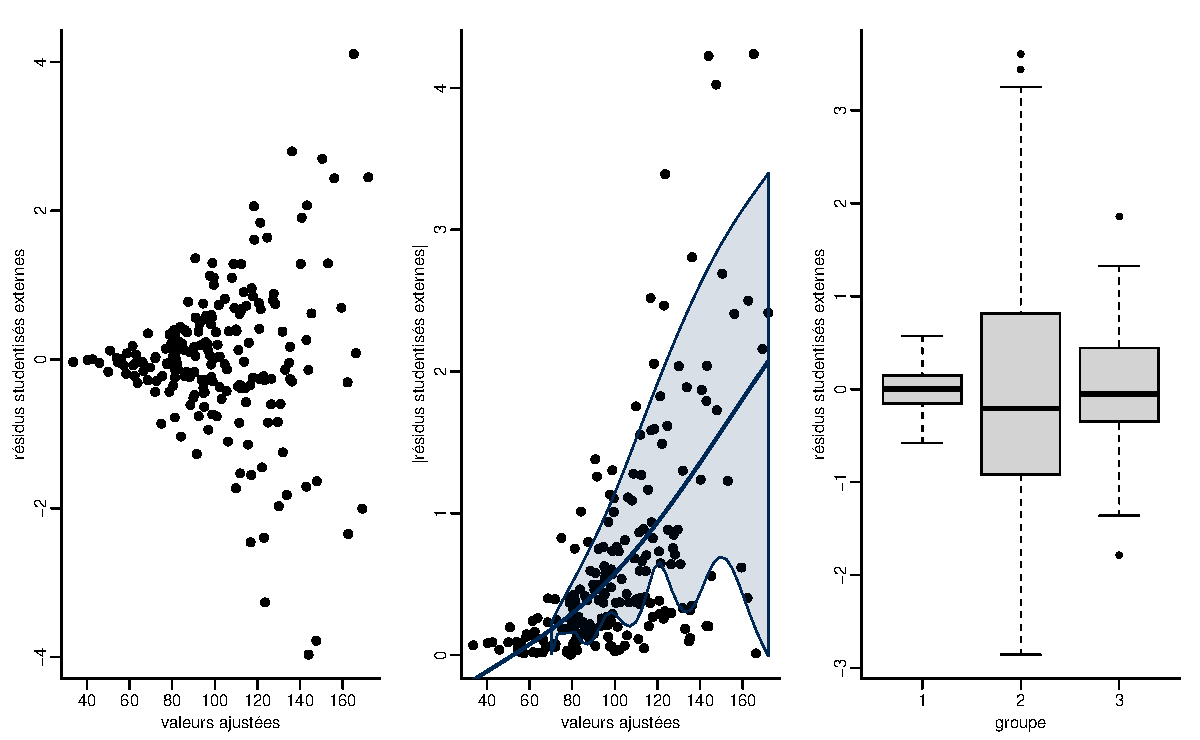
\includegraphics[width=0.85\textwidth,height=\textheight]{regression-lineaire_files/figure-pdf/fig-diagfitvalhomosce-1.pdf}

}

\caption{\label{fig-diagfitvalhomosce}Diagrammes des résidus studentisés
externes en fonction des valeurs ajustées (gauche) et d'une variable
catégorielle (droite).}

\end{figure}%

Une extension évidente du modèle linéaire consiste à permettre à la
variance de varier en fonction des variables explicatives, généralement
des covariables catégorielles. Cela est facile à faire en modifiant la
vraisemblance et nous couvrirons cette approche plus en détail.

Nous pouvons effectuer des tests d'hypothèse pour l'hypothèse
d'homogénéité (égalité) de la variance. Les tests les plus couramment
utilisés sont le test de Bartlett, un test du rapport de vraisemblance
sous l'hypothèse que les données sont tirées d'une loi normale, avec une
correction de Bartlett pour améliorer l'approximation \(\chi^2\) de la
distribution nulle. Ce test est cependant sensible aux écarts à la
normalité, et tend à rejeter même quand la variance est constante. Le
deuxième test le plus répandu est le test de Levene (une alternative
plus robuste, moins sensible aux valeurs aberrantes). Pour les deux
tests, la distribution nulle est
\(\mathscr{H}_0 : \sigma^2_1 = \cdots = \sigma^2_K\) contre
l'alternative qu'au moins deux diffèrent. La statistique du test de
Bartlett a une distribution nulle \(\chi^2\) avec \(K-1\) degrés de
liberté, alors que le test de Levene a une distribution \(F\) avec
(\(K-1\), \(n-K\)) degrés de liberté: il est équivalent au calcul de la
statistique \(F\) de l'ANOVA à un facteur avec la valeur absolue des
résidus centrés, \(|y_{ik} - \widehat{\mu}_k|\), comme observations. Un
test populaire plus général est le test de Breusch et Pagan
(\citeproc{ref-Breusch.Pagan:1979}{1979}), qui est un test du score pour
un modèle de régression linéaire pour le carré des résidus ordinaires
\(e_i^2\). Comme les autres tests de score, ce dernier ne nécessite pas
d'ajustement du modèle avec des variances inégales, mais on doit choisir
quelles variables explicatives mettre dans le modèle.

\begin{example}[Violation du postulat
d'homoscédasticité]\protect\hypertarget{exm-heterogeneity}{}\label{exm-heterogeneity}

~

\begin{figure}[ht!]

\centering{

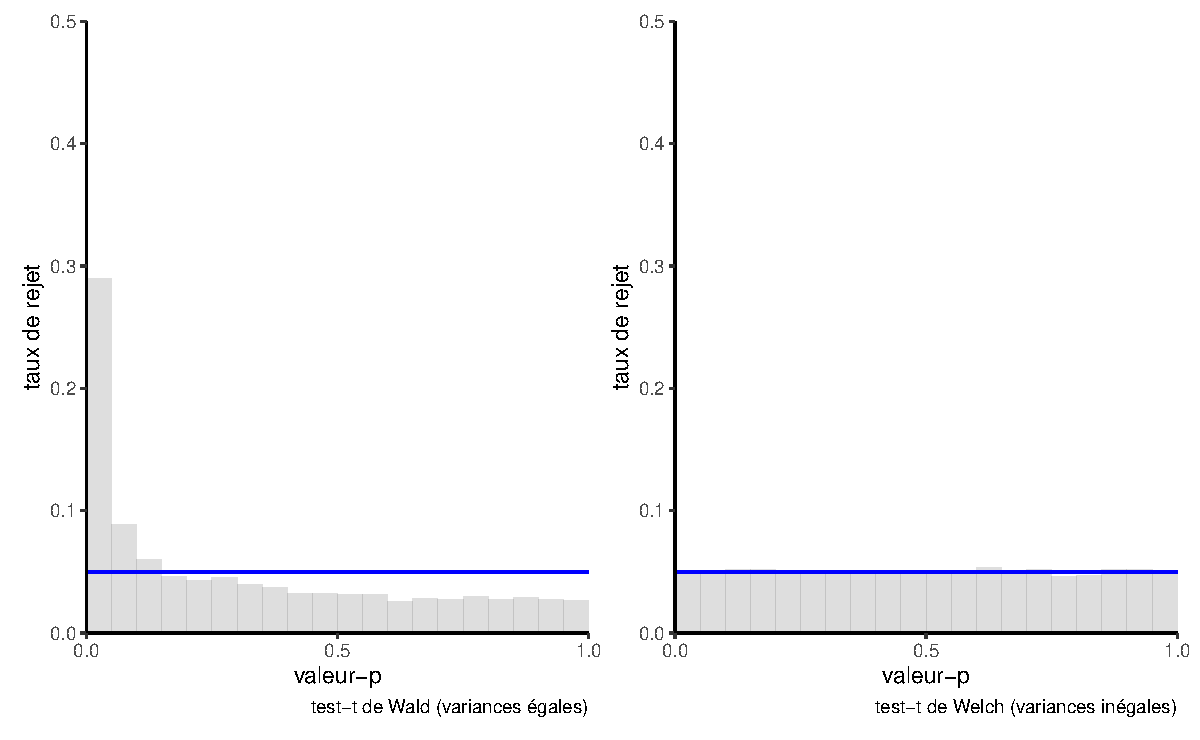
\includegraphics[width=0.85\textwidth,height=\textheight]{regression-lineaire_files/figure-pdf/fig-simuWelchnull-1.pdf}

}

\caption{\label{fig-simuWelchnull}Histogramme de la loi nulle des
valeurs-\(p\) obtenues par simulation à l'aide du test-\(t\) à deux
échantillons (à gauche) et du test-\(t\) de Welch (à droite), sur la
base de 10 000 simulations. Chaque échantillon simulé se compose de 50
observations provenant d'une distribution \(\mathsf{normale}(0, 1)\) et
de 10 observations provenant d'une distribution
\(\mathsf{normale}(0, 9)\). La loi uniforme sous \(\mathscr{H}_0\)
aurait 5 \% dans chacune des 20 cases utilisées pour l'affichage.}

\end{figure}%

Qu'arrive-t-il si la variance est inégale? Considérons un problème
simple de comparaison de moyennes entre deux groupes, qui revient à
effectuer un \(t\)-test pour deux échantillons. Nous avons simulé 50
observations à partir d'une loi \(\mathsf{normale}(0, 1)\) et 10
observations à partir d'une loi \(\mathsf{normale}(0, 9)\), en comparant
la distribution des valeurs \(p\) pour les statistiques du test de Welch
et du test \(t\). En revanche, nous rejetons 0\% du temps avec le
test-\(t\) : il s'agit d'une grande proportion de prémisses erronées
Bien que la distorsion du niveau du test ne soit pas toujours aussi
frappante, l'hétérogénéité doit être prise en compte dans l'élaboration
du modèle en exigeant des tailles d'échantillon suffisantes (lorsque les
coûts le permettent) dans chaque groupe pour pouvoir estimer la variance
de manière fiable dans chaque sous-groupe et à l'aide d'une statistique
adéquate.

\end{example}

Souvent, une variance inégale se produit parce que le modèle n'est pas
additif. Vous pouvez utiliser des transformations stabilisant la
variance (par exemple, pour des effets multiplicatifs) afin de garantir
une variance à peu près égale dans chaque groupe. Dans ce cas de figure,
une transformation logarithmique (ou une transformation de Box--Cox)
peut aider à stabiliser la variance, mais il faut que la réponse soit
positive. Une autre option consiste à utiliser un modèle adapté au type
de réponse que vous avez (y compris les données de décompte et les
données binaires). Enfin, il peut être nécessaire de modéliser
explicitement la variance dans des modèles plus complexes (y compris les
mesures répétées) lorsqu'il y a un effet d'apprentissage au fil du temps
et que la variabilité diminue en conséquence. Consultez un expert si
nécessaire.

Les économistes utilisent fréquemment des estimateurs \textbf{sandwich}
(\citeproc{ref-White:1980}{White 1980}), en remplaçant l'estimateur
usuel de la matrice de covariance des \(\widehat{\boldsymbol{\beta}}\),
d'ordinaire \(S^2(\mathbf{X}^\top\mathbf{X})^{-1}\), par un estimateur
sandwich de la forme
\[\widehat{\mathsf{Va}}_{\mathsf{HCE}}(\boldsymbol{\widehat{\beta}}) = (\mathbf{X}^\top\mathbf{X})^{-1}\mathbf{X}^\top\boldsymbol{\Omega}\mathbf{X}(\mathbf{X}^\top\mathbf{X})^{-1}\]
avec \(\boldsymbol{\Omega}\) une matrice diagonale. Les choix populaires
pour des matrices convergente en cas d'hétéroscédasticité matrices
(\citeproc{ref-McKinnon.White:1985}{MacKinnon et White 1985}), utilisent
\(\mathrm{diag}(\boldsymbol{\Omega})_i = e_i^2/(1-h_{ii})^2\), dans le
cas de la matrice \(\mathrm{HC}_3\).

\subsection{Postulat d'indépendance}\label{postulat-dinduxe9pendance}

Habituellement, l'indépendance des observations découle directement du
type d'échantillonnage utilisé --- cette hypothèse est implicitement
vraie si les observations représentent un \emph{échantillon aléatoire}
de la population. Ce n'est généralement pas le cas pour les données
longitudinales, qui contiennent des mesures répétées des mêmes individus
au fil du temps. De même, les séries temporelles ne sont pas constituées
d'observations indépendantes. Si nous voulons inclure tous les points
temporels dans l'analyse, nous devons tenir compte de l'éventuelle
dépendance (corrélation) entre les observations.

Quel est l'impact de la dépendance entre les mesures? D'un point de vue
heuristique, les mesures corrélées contiennent moins d'informations que
les mesures indépendantes. Dans le cas le plus extrême, il n'y a pas
d'information supplémentaire et les mesures sont identiques, mais le
fait de les ajouter plusieurs fois gonfle indûment la la taille de
l'échantillon. Si nous ignorons la corrélation, les erreurs-type
estimées sont trop petites, car la taille effective de l'échantillon est
inférieure au nombre d'observations. Cela enfle la statistique et
conduit à des rejets plus fréquents des hypothèses nulles, par erreur.

\begin{figure}[ht!]

\centering{

\includegraphics[width=0.85\textwidth,height=\textheight]{regression-lineaire_files/figure-pdf/fig-plotLevelIndep-1.pdf}

}

\caption{\label{fig-plotLevelIndep}Taux de rejet de l'hypothèse nulle
pour le test \(F\) d'égalité des moyennes pour une ANOVA à une voie avec
des données générées en groupes de cinq avec une moyenne et une variance
constantes, à partir d'un modèle d'équicorrélation (les observations à
l'intérieur d'un groupe sont corrélées, les observations entre les
groupes sont indépendantes). Le niveau nominal du test est de 5\%.}

\end{figure}%

Le manque d'indépendance peut également avoir des conséquences
dramatiques sur l'inférence et conduire à de fausses conclusions: la
Figure~\ref{fig-plotLevelIndep} montre un exemple avec des échantillons
corrélés au sein d'un groupe (ou, de manière équivalente, des mesures
répétées d'individus) avec cinq observations par groupe. L'axe des
ordonnées montre la proportion de fois où l'hypothèse nulle est rejetée
alors qu'elle ne devrait l'être en principe que 5\% du temps. Ici, comme
les données sont générées à partir du modèle nul (moyenne égale) avec
une variance égale, l'inflation du nombre d'erreurs de type I est
alarmante et l'inflation du niveau du test est substantielle même avec
une corrélation très limitée entre les mesures.

La première source de dépendance est constituée par les données
groupées, c'est-à-dire les mesures prises sur des sujets qui ne sont pas
indépendants les uns des autres (famille, groupes, etc.) On distingue
entre \textbf{données longitudinales}, qui sont des mesures répétées
sont effectuées sur les mêmes sujets (quelques points temporels) et
\textbf{séries chronologiques}, dont la longueur et la fréquence
d'échantillonage est plus élevée. Les séries temporelles nécessitent des
modèles spécifiques qui ne sont pas abordés dans ce cours. En raison de
l'autocorrélation, les erreurs positives ont tendance à être suivies
d'erreurs positives, etc. Nous pouvons tracer les résidus en fonction du
temps et un nuage de points des résidus retardés \(e_i\) par rapport à
\(e_{i-1}\) (\(i=2, \ldots, n\)).

\begin{figure}[ht!]

\centering{

\includegraphics[width=0.85\textwidth,height=\textheight]{regression-lineaire_files/figure-pdf/fig-timeresidplot-1.pdf}

}

\caption{\label{fig-timeresidplot}Nuage de point de résidus versus les
résidus décalés d'une observation: il n'y a aucune preuve d'indépendance
dans le panneau de gauche, alors que le panneau de droite montre des
résidus positivement corrélés.}

\end{figure}%

Toutefois, les diagrammes de résidus décalés ne montrent que la
dépendance au premier décalage entre les observations. Pour les séries
temporelles, nous pouvons utiliser un corrélogramme, c'est-à-dire un
diagramme à bandes de la corrélation entre deux observations distantes
de \(h\) unités en fonction du décalage
\(h\).(\citeproc{ref-Brockwell.Davis:2016}{Brockwell et Davis 2016},
Definition 1.4.4).

Pour \(y_1, \ldots, y_n\) et des pas de décalages \(h=0, 1, \ldots\),
l'autocorrélation au pas de temps \(h\) est \begin{align*}
r(h) = \frac{\gamma(h)}{\gamma(0)}, \qquad \gamma(h) = \frac{1}{n}\sum_{i=1}^{n-|h|} (y_i-\overline{y})(y_{i+h} - \overline{y})
\end{align*}

Si la série est corrélée, l'autocorrélation de l'échantillon se situera
probablement en dehors des intervalles de confiance ponctuels, comme le
montre la Figure~\ref{fig-correlogram}. La présence d'autocorrélation
nécessite de modéliser la corrélation entre les observations de manière
explicite à l'aide d'outils spécifiques issus de la littérature sur les
séries temporelles. Nous examinerons toutefois les modèles
\(\mathsf{AR}(1)\) dans le cadre du chapitre sur les données
longitudinales. Voir
\href{https://otexts.com/fpp2/regression-evaluation.html}{Forecasting :
Principles and Practice, section 5.3} pour plus de détails.

Lorsque les observations sont positivement corrélées, les erreurs-types
estimées indiquées par le logiciel sont trop petites. Cela signifie que
nous sommes trop confiants et que nous rejetterons l'hypothèse nulle
plus souvent que nous ne le devrions si l'hypothèse nulle était vraie
(erreur de type I gonflée, plus de faux positifs).

\begin{figure}[ht!]

\centering{

\includegraphics[width=0.85\textwidth,height=\textheight]{regression-lineaire_files/figure-pdf/fig-correlogram-1.pdf}

}

\caption{\label{fig-correlogram}Corrélogramme d'observations
indépendantes (à gauche) et des résidus ordinaires du modèle
log-linéaire ajusté aux données sur le traffic aérien (à droite). Alors
que le modèle moyen de ce dernier est apparemment correctement spécifié,
il existe une dépendance résiduelle entre les observations mensuelles et
annuelles (décalage de \(h=12\) mois). Les lignes traitillées en bleu
indiquent un intervalle de confiance ponctuels approximatifs à 95 \%
pour un bruit blanc (observations non corrélées).}

\end{figure}%

Comment prendre en compte la dépendance entre observations? L'idée
principale est de modéliser la corrélation et la variance, en partant du
vecteur complet d'observations et en supposant que
\[\boldsymbol{Y} \mid \mathbf{X} \sim \mathsf{normale}_n(\mathbf{X}\boldsymbol{\beta}, \boldsymbol{\Sigma})\]
avec un modèle pour la matrice de variance de dimension \(n \times n\),
disons \(\boldsymbol{\Sigma}\), qui sera paramétré en fonction de
\(\boldsymbol{\psi}\).

\subsection{Postulat de normalité}\label{postulat-de-normalituxe9}

Le postulat de normalité des aléas est commode, mais pas strictement
nécessaire dans la majorité des cas pour la validité des tests sur les
coefficients ou les énoncés reliés à la moyenne prédite. Si les aléas
suivent une loi normale, les estimateurs des moindres carrés et du
maximum de vraisemblance de \(\boldsymbol{\beta}\) coïncident. Les
estimateurs du maximum de vraisemblance de \(\boldsymbol{\beta}\) sont
asymptotiquement normaux sous de faibles conditions sur la matrice du
modèle et les \(t\)-tests sont étonnamment robustes et ne sont pas
affectés par un écart par rapport au postulat de normalité. Cela
signifie que l'inférence est valable avec de grands échantillons, quelle
que soit la distribution des erreurs/résidus (même si la loi nulle n'est
pas exacte). L'inférence sera valable avec de grands échantillons même
si les aléas ne sont pas normaux à cause du théorème de la limite
centrale. Il est important de garder à l'esprit que, pour les variables
explicatives catégorielles, la taille de l'échantillon dans chaque
sous-groupe doit être suffisamment importante pour que le théorème de la
limite centrale s'applique, puisque les coefficients représentent la
moyenne du sous-groupe. En revanche, les résultats et tests qui
capitalisent sur la loi des aléas (par exemple, les tests pour les
aberrances basés sur le maximum des résidus studentisés, ou les
intervalles de prédictions) seront probablement trompeurs.

Parfois, des transformations peuvent améliorer la normalité : si les
données sont asymétriques à droite et que la variable réponse est
strictement positive, un modèle log-linéaire peut être plus adéquat
Section~\ref{sec-transfo}. Ceci peut être évalué en regardant le
diagramme quantile-quantile des résidus studentisés externes. Si la
réponse \(Y\) n'est pas continue (y compris les données binaires,
proportionnelles ou de dénombrement), les modèles linéaires généralisés
sont plus appropriés.

Si l'aléa \(\varepsilon_i \sim \mathsf{normale}(0, \sigma^2)\), alors
les résidus studentisés externes devraient suivre une distribution de
Student, avec \(r_i \sim \mathsf{Student}(n-p-2)\) (identiquement
distribués, mais non indépendants). Un diagramme quantile-quantile de
Student peut donc être utilisé pour vérifier le postulat. Gardez à
l'esprit que si le modèle de la moyenne ou de la variance n'est pas
correctement spécifié, certains résidus peuvent incorporer les effets
résiduels.

\begin{figure}[ht!]

\centering{

\includegraphics[width=0.85\textwidth,height=\textheight]{regression-lineaire_files/figure-pdf/fig-qqplotresid-1.pdf}

}

\caption{\label{fig-qqplotresid}Histogramme et estimation de densité par
lissage de noyau (gauche) et diagramme quantile-quantile Student
(droite). Le panneau de gauche montre la loi théorique Student (en bleu)
pour comparaison. Le panneau de droite présente des intervalles de
confiance ponctuels à 95\% calculés à l'aide d'un autoamorçage
paramétrique.}

\end{figure}%

Les graphiques quantile-quantile sont abordés dans la
Définition~\ref{def-diagramme-qq}, mais leur interprétation nécessite de
la pratique. Par exemple, la Figure~\ref{fig-qqplotsbad} montre de
nombreux scénarios courants qui peuvent être détectés à l'aide de
diagrammes quantile-quantile. Les données discrètes sont responsables
des motifs en escalier, les données asymétriques à droite ont des
quantiles bas trop élevés et des quantiles hauts trop bas par rapport
aux positions de tracé, les données à ailes lourdes ont des observations
élevées de part et d'autre et les données bimodales conduisent à des
sauts dans le tracé.

\begin{figure}[ht!]

\centering{

\includegraphics[width=0.85\textwidth,height=\textheight]{regression-lineaire_files/figure-pdf/fig-qqplotsbad-1.pdf}

}

\caption{\label{fig-qqplotsbad}Diagrammes quantiles-quantiles de données
discrète (coin supérieur gauche), à ailes lourdes (coin supérieur
droit), asymmétrique à droite (coin inférieur gauche) et bimodales (coin
inférieur droit).}

\end{figure}%

\begin{example}[Diagnostics graphiques pour l'inéquité
salariale]\protect\hypertarget{exm-diagplotcollege}{}\label{exm-diagplotcollege}

On considère le modèle pour les données \texttt{college} avec toutes les
observations (sans interaction) pour voir si les postulats tiennent la
route.

\begin{figure}[ht!]

\centering{

\includegraphics[width=0.85\textwidth,height=\textheight]{regression-lineaire_files/figure-pdf/fig-diagplotscollege-1.pdf}

}

\caption{\label{fig-diagplotscollege}Diagnostic plots for the college
data example: ordinary residuals against fitted values (top left),
absolute value of the jacknnife studentized residuals against fitted
values (top right), box and whiskers plot of jacknnife studentized
residuals (bottom left) and detrended Student quantile-quantile plot
(bottom right). There is clear group heteroscedasticity.}

\end{figure}%

Sur la base des graphiques de Figure~\ref{fig-diagplotscollege}, nous
constatons qu'il existe une hétéroscédasticité au sein des échelons.
Comme le nombre d'années pour les adjoint(e)s est limité et que tous les
professeurs assistants ont été embauchés au cours des six dernières
années, il y a moins de disparité dans leurs revenus. Il est important
de ne pas confondre le modèle sur l'axe \(x\) pour la valeur ajustée (en
raison de l'effet important du rang et du domaine, tous deux variables
catégorielles) avec les modèles dans les résidus (aucun n'est apparent).
La correction de l'hétéroscédasticité permettrait de corriger les
résidus et d'améliorer l'aspect du graphique quantile-quantile.

On effectue quelques tests avec les résidus studentisés externes pour
les données \texttt{college} pour valider ce que les diagnostics
graphiques indiquent.

\begin{Shaded}
\begin{Highlighting}[]
\NormalTok{r }\OtherTok{\textless{}{-}} \FunctionTok{rstudent}\NormalTok{(modlin1\_college)}
\CommentTok{\# Test F de Levene}
\NormalTok{car}\SpecialCharTok{::}\FunctionTok{leveneTest}\NormalTok{(r }\SpecialCharTok{\textasciitilde{}}\NormalTok{ echelon, }\AttributeTok{center =} \StringTok{"mean"}\NormalTok{, }\AttributeTok{data =}\NormalTok{ college)}
\CommentTok{\#\textgreater{} Levene\textquotesingle{}s Test for Homogeneity of Variance (center = "mean")}
\CommentTok{\#\textgreater{}        Df F value Pr(\textgreater{}F)    }
\CommentTok{\#\textgreater{} group   2      50 \textless{}2e{-}16 ***}
\CommentTok{\#\textgreater{}       394                   }
\CommentTok{\#\textgreater{} {-}{-}{-}}
\CommentTok{\#\textgreater{} Signif. codes:  0 \textquotesingle{}***\textquotesingle{} 0.001 \textquotesingle{}**\textquotesingle{} 0.01 \textquotesingle{}*\textquotesingle{} 0.05 \textquotesingle{}.\textquotesingle{} 0.1 \textquotesingle{} \textquotesingle{} 1}
\CommentTok{\# Test du score avec Breusch{-}Pagan}
\NormalTok{car}\SpecialCharTok{::}\FunctionTok{ncvTest}\NormalTok{(modlin1\_college, }\AttributeTok{var.formula =}  \SpecialCharTok{\textasciitilde{}}\NormalTok{ echelon)}
\CommentTok{\#\textgreater{} Non{-}constant Variance Score Test }
\CommentTok{\#\textgreater{} Variance formula: \textasciitilde{} echelon }
\CommentTok{\#\textgreater{} Chisquare = 70.2, Df = 2, p = 6e{-}16}
\end{Highlighting}
\end{Shaded}

Pour les données de collège, on spécifie donc plutôt
\(Y_i \sim \mathsf{normale}(\mathbf{x}_i\boldsymbol{\beta}, \sigma^2_{\texttt{echelon}_i})\)
avec un paramètre de variance spécifique à l'échelon. Cela semble
corriger l'hétéroscédasticité.

\begin{Shaded}
\begin{Highlighting}[]
\FunctionTok{library}\NormalTok{(nlme) }\CommentTok{\# modèles mixtes et structures de corrélation}
\NormalTok{modlin.college2 }\OtherTok{\textless{}{-}}\NormalTok{ nlme}\SpecialCharTok{::}\FunctionTok{gls}\NormalTok{(}
  \AttributeTok{model =}\NormalTok{ salaire }\SpecialCharTok{\textasciitilde{}}\NormalTok{ echelon }\SpecialCharTok{+}\NormalTok{ domaine }\SpecialCharTok{+}\NormalTok{ sexe }\SpecialCharTok{+}\NormalTok{ service, }\CommentTok{\# spécification de la moyenne}
  \AttributeTok{weights =}\NormalTok{ nlme}\SpecialCharTok{::}\FunctionTok{varIdent}\NormalTok{(}\AttributeTok{form =} \SpecialCharTok{\textasciitilde{}}\DecValTok{1} \SpecialCharTok{|}\NormalTok{ echelon), }\CommentTok{\# variance constante par échelon}
  \AttributeTok{data =}\NormalTok{ college)}
\FunctionTok{plot}\NormalTok{(modlin.college2)}
\NormalTok{car}\SpecialCharTok{::}\FunctionTok{Anova}\NormalTok{(modlin.college2)}
\CommentTok{\#\textgreater{} Analysis of Deviance Table (Type II tests)}
\CommentTok{\#\textgreater{} }
\CommentTok{\#\textgreater{} Response: salaire}
\CommentTok{\#\textgreater{}         Df  Chisq Pr(\textgreater{}Chisq)    }
\CommentTok{\#\textgreater{} echelon  2 363.50     \textless{}2e{-}16 ***}
\CommentTok{\#\textgreater{} domaine  1  91.04     \textless{}2e{-}16 ***}
\CommentTok{\#\textgreater{} sexe     1   1.80      0.180    }
\CommentTok{\#\textgreater{} service  1   2.97      0.085 .  }
\CommentTok{\#\textgreater{} {-}{-}{-}}
\CommentTok{\#\textgreater{} Signif. codes:  0 \textquotesingle{}***\textquotesingle{} 0.001 \textquotesingle{}**\textquotesingle{} 0.01 \textquotesingle{}*\textquotesingle{} 0.05 \textquotesingle{}.\textquotesingle{} 0.1 \textquotesingle{} \textquotesingle{} 1}
\end{Highlighting}
\end{Shaded}

\begin{center}
\includegraphics[width=0.85\textwidth,height=\textheight]{regression-lineaire_files/figure-pdf/unnamed-chunk-59-1.pdf}
\end{center}

Le modèle est ajusté par maximum de vraisemblance restreint avec la
fonction \texttt{gls} du paquet \texttt{nlme}. La modification semble
suffisante pour capturer l'hétéroscédasticité dans le diagramme des
résidus standardisés vs valeurs ajustées.

On pourrait aussi essayer d'utiliser la matrice sandwich, en remplaçant
l'estimateur de \(\mathsf{Va}(\widehat{\boldsymbol{\beta}})\) par
\(\widehat{\mathsf{Va}}_{\mathsf{HCE}}(\boldsymbol{\widehat{\beta}})\)
dans la formule des tests de Wald. Ici, c'est option n'est pas
recommandée car moins efficace.

\begin{Shaded}
\begin{Highlighting}[]
\CommentTok{\# Matrice de covariance sandwich}
\NormalTok{vcov\_HCE }\OtherTok{\textless{}{-}}\NormalTok{ car}\SpecialCharTok{::}\FunctionTok{hccm}\NormalTok{(modlin1\_college)}
\CommentTok{\# Statistiques de Wald}
\NormalTok{lmtest}\SpecialCharTok{::}\FunctionTok{coeftest}\NormalTok{(modlin1\_college, }\AttributeTok{vcov. =}\NormalTok{ vcov\_HCE)}
\end{Highlighting}
\end{Shaded}

\end{example}

\subsection{Transformation de la variable réponse}\label{sec-transfo}

Si la réponse est strictement positive, certaines options peuvent
atténuer le manque d'additivité, plus particulièrement les relations
multiplicatives entre la moyenne et la variance. Si les données sont
asymétriques et que la réponse est strictement positive, un modèle
log-linéaire peut être plus approprié et les paramètres peuvent être
interprétés.

Écrivons le modèle log-linéaire \begin{align*}
\ln Y = \beta_0+ \beta_1 X_1 +\cdots + \beta_pX_p + \varepsilon;
\end{align*} à l'échelle originale de la variable réponse, cela
représente \begin{align*}
Y &= \exp\left(\beta_0 +\beta_1 X_1 +\cdots + \beta_pX_p\right)\cdot \exp(\varepsilon),
\end{align*} et donc \begin{align*}
\mathsf{E}(Y \mid \mathbf{X}) = \exp(\beta_0 +\beta_1 X_1 +\cdots + \beta_pX_p) \times \mathsf{E}\{\exp(\varepsilon) \mid \mathbf{X}\}.
\end{align*} Si
\(\varepsilon \mid \mathbf{x} \sim \mathsf{normale}(\mu,\sigma^2)\),
alors
\(\mathsf{E}\{\exp(\varepsilon) \mid \mathbf{x}\}= \exp(\mu+\sigma^2/2)\)
et \(\exp(\varepsilon)\) suit une loi lognormale. Une augmentation d'une
unité de \(X_j\) mène à une augmentation moyenne de \(\beta_j\) de
\(\ln Y\) sans interaction ni terme nonlinéaire pour \(X_j\), et cela se
traduit par un facteur multiplicatif de \(\exp(\beta_j)\) à l'échelle de
\(Y\). Si \(\beta_j=0\), \(\exp(\beta_j)=1\) et il n'y a pas de
changement, si \(\beta_j < 0\), \(\exp(\beta_j)<1\) et la moyenne
décroît avec \(X_j\), et si \(\beta_j > 0\), \(\exp(\beta_j)>1\) et la
moyenne augmente avec \(X_j\).

Comparez le rapport \begin{align*}
\frac{\mathsf{E}(Y \mid X_1=x+1, X_2, \ldots, X_p)}{\mathsf{E}(Y \mid X_1=x,  X_2, \ldots, X_p)} = \frac{\exp\{\beta_1(x+1)\}}{\exp(\beta_1 x)} = \exp(\beta_1).
\end{align*} Ainsi, \(\exp(\beta_1)\) donne le rapport des moyennes de
\(Y\) quand \(X_1=x+1\) par rapport à \(X_1=x\), \emph{ceteris paribus}
(avec les restrictions habituelles). L'interprétation (par rapport à la
référence, dépend du signe de \(\beta_j\): le pourcentage de diminution
est \(1-\exp(\beta_j)\) si \(\beta_j <0\) et le pourcentage
d'augmentation est \(\exp(\beta_j)-1\) si \(\beta_j>0\).

Parfois, on veut considérer une transformation à la fois de la réponse
et d'une variable explicative positive continue, un modèle log-log.
Considérons le cas où on prend le logarithme de \(Y\) et \(X_1\), avec
\begin{align*}
Y= X_1^{\beta_1}\exp(\beta_0 + \beta_2X_2 + \cdots + \beta_pX_p + \varepsilon)
\end{align*} En prenant la dérivée par rapport à \(X_1>0\), on obtient
\begin{align*}
\frac{\partial Y}{\partial X_1}&= \beta_1 X_1^{\beta_1-1}\exp(\beta_0 + \beta_2X_2 + \cdots + \beta_pX_p + \varepsilon)\\&= \frac{\beta_1 Y}{X_1}
\end{align*} et réarranger cette expression nous donne \begin{align*}
\frac{\partial X_1}{X_1}\beta_1 = \frac{\partial Y}{Y};
\end{align*} une mesure \textbf{d'élasticité partielle}: le coefficient
\(\beta_1\) est un pourcentage de changement de \(Y\) pour chaque
pourcentage d'augmentation de \(X_1\), \emph{ceteris paribus}.

\begin{example}[Modèle de
Cobb-Douglas]\protect\hypertarget{exm-loglog}{}\label{exm-loglog}

Considérons par exemple la fonction de production Cobb--Douglas
(\citeproc{ref-Douglas:1976}{Douglas 1976}), qui spécifie que la
production économique \(Y\) est liée au travail \(L\) et au capital
\(C\) par l'intermédiaire de
\(\mathsf{E}(Y \mid L, C) = \beta_0C^{\beta}L^{1-\beta}\) avec
\(\beta \ dans (0,1)\).Si nous prenons les logarithmes des deux côtés
(puisque tous les arguments sont positifs), alors
\(\mathsf{E}(\ln Y \mid L, C) = \beta_0^* + \beta_1 \ln C + (1-\beta_1)\ln L\).
Nous pourrions ajuster un modèle linéaire avec la réponse
\(\ln Y - \ln L\) et la variable explicative \(\ln C - \ln L\), pour
obtenir une estimation du coefficient \(\beta_1\), tandis que
\(\beta_0^*=\ln \beta_0\). Une optimisation sous contrainte serait
potentiellement nécessaire pour estimer les paramètres du modèle
linéaire résultant si les estimations se situent en dehors de l'espace
des paramètres.

\end{example}

\begin{proposition}[Transformation de
Box--Cox]\protect\hypertarget{prp-boxcox}{}\label{prp-boxcox}

Avec des données strictement positives, on peut utiliser une
transformation de Box--Cox (\citeproc{ref-Box.Cox:1964}{Box et Cox
1964}), \begin{align*}
y(\lambda)= \begin{cases}
(y^{\lambda}-1)/\lambda, & \lambda \neq 0\\
\ln(y), & \lambda=0.
\end{cases}
\end{align*} Les cas de figure \(\lambda=-1\) (inverse), \(\lambda=1\)
(identité) et \(\lambda=0\) (logarithme) sont les plus importants car
les modèles résultants sont interprétables.

Si on suppose que
\(\boldsymbol{Y}(\lambda) \sim \mathsf{normale}(\mathbf{X}\boldsymbol{\beta}, \sigma^2 \mathbf{I}_n)\),
alors la vraisemblance est \begin{align*}
L(\lambda, \boldsymbol{\beta}, \sigma; \boldsymbol{y}, \mathbf{X}) &= (2\pi\sigma^2)^{-n/2} J(\lambda, \boldsymbol{y}) \times\\& \quad \exp \left[ - \frac{1}{2\sigma^2}\{\boldsymbol{y}(\lambda) - \mathbf{X}\boldsymbol{\beta}\}^\top\{\boldsymbol{y}(\lambda) - \mathbf{X}\boldsymbol{\beta}\}\right],
\end{align*} où \(J\) dénote le Jacobien de la transformation Box--Cox,
\(J(\lambda, \boldsymbol{y})=\prod_{i=1}^n y_i^{\lambda-1}\).

\section{\texorpdfstring{Profilage de
\(\lambda\)}{Profilage de \textbackslash lambda}}\label{profilage-de-lambda}

Pour chaque valeur de \(\lambda\), on obtient les estimateurs du maximum
de vraisemblance usuels en remplaçant \(\boldsymbol{y}\) par
\(\boldsymbol{y}(\lambda)\).

La log vraisemblance profilée pour \(\lambda\) est \begin{align*}
\ell_{\mathsf{p}}(\lambda) = -\frac{n}{2}\ln(2\pi \widehat{\sigma}^2_\lambda) - \frac{n}{2} + (\lambda - 1)\sum_{i=1}^n \ln(y_i)
\end{align*}

Nous ne pouvons pas comparer les modèles ajustés à \(Y_i\) par rapport à
\(\ln Y_i\) en utilisant, par exemple, des critères d'information ou des
tests, parce que les modèles ont des réponses différentes. Nous pouvons
toutefois utiliser la vraisemblance de Box--Cox, qui inclut le
\textbf{Jacobien} de la transformation, pour évaluer la qualité de
l'ajustement et comparer le modèle avec \(\lambda=1\) par rapport à
\(\lambda=0\).

La transformation de Box-Cox n'est pas une panacée et doit être réservée
aux cas où la transformation réduit l'hétéroscédasticité (variance
inégale) ou crée une relation linéaire entre les explications et la
réponse : la théorie fournit une explication convaincante des données.
Plutôt qu'un choix \emph{ad hoc} de transformation, on pourrait prendre
une transformation logarithmique si la valeur 0\$ est incluse dans
l'intervalle de confiance à 95\%, car cela améliore l'interprétabilité.

\end{proposition}

\begin{example}[Transformation de Box--Cox pour données sur les
poisons]\protect\hypertarget{exm-poisonboxcox}{}\label{exm-poisonboxcox}

Box et Cox (\citeproc{ref-Box.Cox:1964}{1964}) modélisent le temps de
survie de 48 animaux sur la base d'un essai aléatoire. Les données sur
les \texttt{poisons} sont équilibrées, 3 poisons ayant été administrés
avec 4 traitements à 4 animaux chacun. Nous pourrions envisager une
ANOVA à deux facteurs sans interaction, étant donné le peu
d'observations pour chaque combinaison. Le modèle s'écrit alors
\begin{align*}
Y &= \beta_0 + \beta_1 \texttt{poison}_2 + \beta_2\texttt{poison}_3  +\beta_3\texttt{treatment}_2 \\ &\qquad+ \beta_4\texttt{treatment}_3
+\beta_5\texttt{treatment}_4 + \varepsilon
\end{align*}

Le tracé des valeurs ajustées par rapport aux résidus montre que le
modèle n'est pas additif (panneau du milieu de la
Figure~\ref{fig-poisonplots}); il y a également des indications que la
variance augmente avec la réponse moyenne. Le modèle est inadéquat: les
temps de survie les plus faibles sont sous-estimés, ce qui signifie que
les résidus sont positifs, de même que les réponses moyennes. Un test
formel de non-additivité indique également la non-additivité
(\citeproc{ref-Davison:2003}{Davison 2003}, Exemple 8.24). Dans
l'ensemble, l'ajustement du modèle est médiocre et toute conclusion
tirée de celui-ci est douteuse.

On pourrait envisager d'utiliser un Box--Cox pour trouver une
transformation appropriée des résidus afin d'améliorer la normalité. Une
analyse des résidus dans les quatre premiers graphiques de
Figure~\ref{fig-poisonplots} montre des signes d'hétéroscédasticité en
fonction du poison et du traitement. Ceci est évident en regardant le
graphique des résidus ordinaires, qui montre une augmentation de la
variance avec le temps de survie. Le tracé quantile-quantile dans le
tracé du milieu à droite montre quelques signes d'écart par rapport à la
normalité, mais la non-linéarité et l'hétéroscédasticité le masquent.

\begin{figure}[ht!]

\centering{

\includegraphics[width=0.85\textwidth,height=\textheight]{regression-lineaire_files/figure-pdf/fig-poisonplots-1.pdf}

}

\caption{\label{fig-poisonplots}Diagnostics graphiques pour les données
de poisons. Panneau du haut: vraisemblance profilée pour \(\lambda\).
Panneau du milieu: (\(\lambda=1\), temps de survie) et du bas
\((\lambda=-1\), vitesse d'absorption). Les diagnostics pour les modèles
représentent les résidus ordinaires versus valeurs ajustées et diagramme
quantile-quantile des résidus studentisés.}

\end{figure}%

L'intervalle de confiance à 95\% basé sur la log-vraisemblance profilée
pour le paramètre du modèle Box--Cox contient \(\lambda=-1\). La
réciproque de la variable réponse \(Y^{-1}\) indique la vitesse d'action
du poison, selon le type et le traitement. Les diagnostics graphiques de
ce modèles, présentés dans le panneau du bas de la
Figure~\ref{fig-poisonplots} ne montrent aucune structure résiduelle.

\end{example}

\bookmarksetup{startatroot}

\chapter*{Bibliographie}\label{bibliographie}
\addcontentsline{toc}{chapter}{Bibliographie}

\markboth{Bibliographie}{Bibliographie}

\phantomsection\label{refs}
\begin{CSLReferences}{1}{0}
\bibitem[\citeproctext]{ref-Baumann:1992}
Baumann, James F., Nancy Seifert-Kessell, et Leah A. Jones. 1992.
{«~Effect of Think-Aloud Instruction on Elementary Students'
Comprehension Monitoring Abilities~»}. \emph{Journal of Reading
Behavior} 24 (2): 143‑72.
\url{https://doi.org/10.1080/10862969209547770}.

\bibitem[\citeproctext]{ref-Box.Cox:1964}
Box, G. E. P., et D. R. Cox. 1964. {«~An Analysis of Transformations~»}.
\emph{Journal of the Royal Statistical Society: Series B
(Methodological)} 26 (2): 211‑43.
\url{https://doi.org/10.1111/j.2517-6161.1964.tb00553.x}.

\bibitem[\citeproctext]{ref-Breusch.Pagan:1979}
Breusch, T. S., et A. R. Pagan. 1979. {«~A Simple Test for
Heteroscedasticity and Random Coefficient Variation~»}.
\emph{Econometrica} 47 (5): 1287‑94.
\url{http://www.jstor.org/stable/1911963}.

\bibitem[\citeproctext]{ref-Brockwell.Davis:2016}
Brockwell, P. J., et R. A. Davis. 2016. \emph{Introduction to Time
Series and Forecasting}. Springer Texts in Statistics. Springer.

\bibitem[\citeproctext]{ref-Brodeur:2021}
Brodeur, Mathieu, Perrine Ruer, Pierre-Majorique Léger, et Sylvain
Sénécal. 2021. {«~Smartwatches are more distracting than mobile phones
while driving: Results from an experimental study~»}. \emph{Accident
Analysis \& Prevention} 149: 105846.
\url{https://doi.org/10.1016/j.aap.2020.105846}.

\bibitem[\citeproctext]{ref-Brucks.Levav:2022}
Brucks, Melanie S., et Jonathan Levav. 2022. {«~Virtual communication
curbs creative idea generation~»}. \emph{Nature} 605 (7908): 108‑12.
\url{https://doi.org/10.1038/s41586-022-04643-y}.

\bibitem[\citeproctext]{ref-Crump.Navarro.Suzuki:2019}
Crump, M. J. C., D. J. Navarro, et J. Suzuki. 2019. \emph{Answering
Questions with Data: Introductory Statistics for Psychology Students}.
\url{https://doi.org/10.17605/OSF.IO/JZE52}.

\bibitem[\citeproctext]{ref-Davison:2003}
Davison, A. C. 2003. \emph{Statistical Models}. Cambridge University
Press.

\bibitem[\citeproctext]{ref-Douglas:1976}
Douglas, Paul H. 1976. {«~The {Cobb--Douglas} Production Function Once
Again: Its History, Its Testing, and Some New Empirical Values~»}.
\emph{Journal of Political Economy} 84 (5): 903‑15.
\url{http://www.jstor.org/stable/1830435}.

\bibitem[\citeproctext]{ref-Duke.Amir:2023}
Duke, Kristen E., et On Amir. 2023. {«~The Importance of Selling
Formats: When Integrating Purchase and Quantity Decisions Increases
Sales~»}. \emph{Marketing Science} 42 (1): 87‑109.
\url{https://doi.org/10.1287/mksc.2022.1364}.

\bibitem[\citeproctext]{ref-Fox:1992}
Fox, John, et Georges Monette. 1992. {«~Generalized Collinearity
Diagnostics~»}. \emph{Journal of the American Statistical Association}
87 (417): 178‑83. \url{https://doi.org/10.1080/01621459.1992.10475190}.

\bibitem[\citeproctext]{ref-Student:1908}
Gosset, William Sealy. 1908. {«~The probable error of a mean~»}.
\emph{Biometrika} 6 (1): 1‑25.
\url{https://doi.org/10.1093/biomet/6.1.1}.

\bibitem[\citeproctext]{ref-Lee.Choi:2019}
Lee, Kiljae, et Jungsil Choi. 2019. {«~Image-text inconsistency effect
on product evaluation in online retailing~»}. \emph{Journal of Retailing
and Consumer Services} 49: 279‑88.
\url{https://doi.org/10.1016/j.jretconser.2019.03.015}.

\bibitem[\citeproctext]{ref-Lin.Kim.Uduehi.Keinan:2024}
Lin, Jason D, Nicole You Jeung Kim, Esther Uduehi, et Anat Keinan. 2024.
{«~Culture for Sale: Unpacking Consumer Perceptions of Cultural
Appropriation~»}. \emph{Journal of Consumer Research}.
\url{https://doi.org/10.1093/jcr/ucad076}.

\bibitem[\citeproctext]{ref-Liu.Rim.Min.Min:2023}
Liu, Peggy J., SoYon Rim, Lauren Min, et Kate E. Min. 2023. {«~The
surprise of reaching out: Appreciated more than we think.~»}
\emph{Journal of Personality and Social Psychology} 124 (4): 754‑71.
\url{https://doi.org/10.1037/pspi0000402}.

\bibitem[\citeproctext]{ref-McKinnon.White:1985}
MacKinnon, James G, et Halbert White. 1985. {«~Some
heteroskedasticity-consistent covariance matrix estimators with improved
finite sample properties~»}. \emph{Journal of Econometrics} 29 (3):
305‑25. \url{https://doi.org/10.1016/0304-4076(85)90158-7}.

\bibitem[\citeproctext]{ref-McCullagh.Nelder:1989}
McCullagh, P., et J. A. Nelder. 1989. \emph{Generalized linear models}.
{S}econd edition. London: Chapman \& Hall.

\bibitem[\citeproctext]{ref-Moon.VanEpps:2023}
Moon, Alice, et Eric M VanEpps. 2023. {«~Giving Suggestions: Using
Quantity Requests to Increase Donations~»}. \emph{Journal of Consumer
Research} 50 (1): 190‑210. \url{https://doi.org/10.1093/jcr/ucac047}.

\bibitem[\citeproctext]{ref-Rosen:1974}
Rosen, B., et T. H. Jerdee. 1974. {«~Influence of sex role stereotypes
on personnel decisions.~»} \emph{Journal of Applied Psychology} 59:
9‑14.

\bibitem[\citeproctext]{ref-Sharma.Tully.Cryder:2021}
Sharma, Eesha, Stephanie Tully, et Cynthia Cryder. 2021.
{«~Psychological Ownership of (Borrowed) Money~»}. \emph{Journal of
Marketing Research} 58 (3): 497‑514.
\url{https://doi.org/10.1177/0022243721993816}.

\bibitem[\citeproctext]{ref-Sokolova:2023}
Sokolova, Tatiana, Aradhna Krishna, et Tim Döring. 2023. {«~Paper Meets
Plastic: The Perceived Environmental Friendliness of Product
Packaging~»}. \emph{Journal of Consumer Research} 50 (3): 468‑91.
\url{https://doi.org/10.1093/jcr/ucad008}.

\bibitem[\citeproctext]{ref-Venables:2000}
Venables, William N. 2000. {«~Exegeses on Linear Models~»}. In
\emph{S-PLUS User's Conference}. Washington, D.C.
\url{https://www.stats.ox.ac.uk/pub/MASS3/Exegeses.pdf}.

\bibitem[\citeproctext]{ref-White:1980}
White, Halbert. 1980. {«~A Heteroskedasticity-Consistent Covariance
Matrix Estimator and a Direct Test for Heteroskedasticity~»}.
\emph{Econometrica} 48 (4): 817‑38.
\url{https://doi.org/10.2307/1912934}.

\end{CSLReferences}


\backmatter


\end{document}
